% !TEX encoding = UTF-8 Unicode
% !BIB TS-program = biber
% !TEX root = main.tex

% Fix for xcolor option clash - Pass table option before class loads it
\PassOptionsToPackage{table,xcdraw}{xcolor}

% --- PDF Metadata & Standards ---
% Note: \DocumentMetadata requires LaTeX 2022-06-01 or newer
% Commented out for compatibility with older TeX Live versions
% \DocumentMetadata 
% {
% 	lang		= en-US,
% 	pdfversion  = 1.7,
% 	pdfstandard = a-2b,
% }

\documentclass[twoside, fontset=newtx, mydesign=mydesign]{mitthesis} 
% fontset=newtx gives professional Times Roman (matches ASU requirement)
% mydesign=mydesign loads the ASU margin settings from mydesign.tex

% --- Essential Packages ---
\usepackage[utf8]{inputenc}
\usepackage[T1]{fontenc}
\usepackage{csquotes}
\usepackage{graphicx}
\usepackage{float}
\usepackage{subcaption}
\graphicspath{{figures/}{figures/Logos/}{figures/Chapter 1/}{figures/Chapter 2/}{figures/Chapter 3/}{figures/Chapter 4/}{figures/Chapter 5/}{figures/Chapter 6/}{figures/Chapter 7/}}

% --- Mathematics & Science ---
\usepackage{amsmath}
\usepackage{mathtools}
\usepackage[version=4]{mhchem}
\usepackage{siunitx}
\sisetup{per-mode=symbol}

% --- Tables ---
\usepackage{booktabs}
\usepackage{array}
\usepackage{multirow}
\usepackage{longtable}
\usepackage{tabularx}
\usepackage{dcolumn}

% Define \degree command
\providecommand{\degree}{\ensuremath{^{\circ}}}

% --- Diagrams ---
\usepackage{tikz}
\usetikzlibrary{shapes, arrows, positioning, calc, fit}

% --- Algorithms ---
\usepackage[ruled,vlined,linesnumbered]{algorithm2e}

% --- Code Listings ---
\usepackage{listings}
\usepackage[table]{xcolor} % Added [table] for \rowcolor support
\definecolor{backcolour}{rgb}{0.95,0.95,0.92}
\definecolor{codegray}{rgb}{0.5,0.5,0.5}
\definecolor{codepurple}{rgb}{0.58,0,0.82}
\definecolor{magenta}{rgb}{1.0,0.0,1.0}

\lstset{
    backgroundcolor=\color{backcolour},   
    commentstyle=\color{codegray},
    keywordstyle=\color{magenta},
    numberstyle=\tiny\color{codegray},
    basicstyle=\ttfamily\footnotesize,
    breaklines=true,                 
    keepspaces=true,                 
    numbers=left,                    
    numbersep=5pt,                  
    frame=lines
}

% --- Boxes ---
\usepackage[most]{tcolorbox}
\definecolor{asuBlue}{RGB}{0, 61, 121}
\newtcolorbox{notebox}{colback=blue!5, colframe=asuBlue, title={\textbf{Note}}, fonttitle=\bfseries, boxrule=1pt, arc=3pt}

% --- Acronyms ---
\usepackage[acronym, toc, nopostdot]{glossaries}
\makeglossaries

% --- Bibliography (MIT Default: BibLaTeX) ---
\usepackage[
    style=numeric-comp, 
    sorting=none, 
    backend=biber, 
    maxbibnames=10, 
    giveninits=true
]{biblatex}
\addbibresource{backmatter/references.bib}

% Remove "In:" for articles (MIT Style)
\renewbibmacro{in:}{%
  \ifentrytype{article}{}{\printtext{\bibstring{in}\intitlepunct}}}

% --- Metadata (Required by mitthesis class) ---
\hypersetup{
    pdfauthor={AUSRA Team},
    pdftitle={Autonomous Unified Swarm Robotics Architecture},
    pdfsubject={Graduation Project 2026}
}

% MIT Thesis Class Variables
% MIT Thesis Class Variables
% MIT Thesis Class Variables (Commented out to prevent unwanted output/checks)
% \Title{Autonomous Unified Swarm Robotics Architecture (AUSRA)}
% \Author{Abdelrahman T. M. Osman et al.}{Mechatronics Engineering}
% \Department{Mechatronics Engineering Program}
% \Degree{Bachelor of Science}{Mechatronics Engineering Program}
% \Supervisor{Dr. Diaa Emad}{Associate Professor}
% \AcceptanceDate{June 2026}
% \DegreeDate{June}{2026}
% \ThesisDate{June 2026}

% --- Headers & Footers (Professional Style) ---
\usepackage{fancyhdr}

% Configure fancy style (for regular pages)
\fancypagestyle{fancy}{
  \fancyhf{} % Clear all
  \setlength{\headheight}{36pt}
  % Static layout: Logo always left, Chapter always right
  \fancyhead[L]{
\includegraphics[height=0.8cm]{figures/Logos/asu_logo.png}}
  \fancyhead[R]{\leftmark}
  \fancyfoot[L]{AUSRA TEAM}
  \fancyfoot[C]{}
  \fancyfoot[R]{\thepage}
  \renewcommand{\headrulewidth}{0.5pt}
  \renewcommand{\footrulewidth}{0.4pt}
}

% Configure plain style (for chapter first pages)
\fancypagestyle{plain}{
  \fancyhf{} % Clear all
  \setlength{\headheight}{14pt} % Minimal for no header
  \fancyfoot[L]{AUSRA TEAM}
  \fancyfoot[C]{}
  \fancyfoot[R]{\thepage}
  \renewcommand{\headrulewidth}{0pt}
  \renewcommand{\footrulewidth}{0.4pt}
}

% Set default to fancy
\pagestyle{fancy}

% Customize chapter and section marks
\renewcommand{\chaptermark}[1]{\markboth{\thechapter.\ #1}{}}
\renewcommand{\sectionmark}[1]{\markright{\thesection.\ #1}}

% ============================================================================
% DOCUMENT BEGINS
% ============================================================================
\begin{document}

% --- Front Matter ---
\pagestyle{empty}
% ============================================================================
% Title Page - Custom Redesign (Ain Shams University)
% ============================================================================

\begin{titlepage}
\thispagestyle{empty}

% --- University & Faculty Header ---
\begin{center}
    {\large\bfseries AIN SHAMS UNIVERSITY}\\[0.2cm]
    {\large\bfseries FACULTY OF ENGINEERING}\\[0.2cm]
    {\large\bfseries MECHATRONICS ENGINEERING PROGRAM}
\end{center}

\vspace{0.3cm}

% --- University Logo ---
\begin{center}
    
\includegraphics[width=3.5cm]{figures/Logos/asu_logo.png}
\end{center}

\vspace{0.3cm}

% --- Project Title ---
\begin{center}
    {\Huge\bfseries\color{asuBlue} Autonomous Unified Swarm Robotics Architecture:}\\[0.3cm]
    {\LARGE\bfseries\color{asuBlue} AUSRA Platform}
\end{center}

\vspace{0.5cm}

% --- Course/Project Subtitle ---
\begin{center}
    {\Large\bfseries Graduation Project 2026}
\end{center}

\vspace{1.0cm}

% --- Team Members (Sorted Alphabetically) ---
\noindent
\begin{minipage}[t]{1.0\textwidth}
    \centering
    {\large\bfseries Prepared by:}\\[0.3cm]
    
    \begin{tabular}{l l}
    \textbf{Abdelrahman Tarek Mohamed Osman} & 2101547 \\
    \textbf{Ahmed Mahmoud Abdelazeem} & 2100718 \\
    \textbf{El Mahdy Salih Ahmed} & 2101875 \\
    \textbf{Mahmoud Atef} & 2001313 \\
    \textbf{Mostafa Samy Mohammed El-Beshlawy} & 2100349 \\
    \textbf{Omar Mohsen Mohamed Attia} & 2100881 \\
    \textbf{Youssef Ahmed Mahmoud Elgharably} & 2101548 \\
    \textbf{Youssef Mostafa Kamel Mohamed} & 2101019 \\
    \textbf{Zaid Reda Farouk Hamed Elmalah} & 2101603 \\
    \end{tabular}
\end{minipage}

\vspace{1.0cm}

% --- Supervisor ---
\begin{center}
    {\Large\bfseries Supervised by:}\\[0.3cm]
    {\Large\color{asuBlue} Dr. Diaa Emad}\\[0.1cm]
    {\small Associate Professor}
\end{center}

\vfill

\end{titlepage}

\clearpage

% Declaration (ASU Specific)
% ============================================================================
% Declaration Page - Compact Single Page
% ============================================================================

\chapter*{Declaration}
\addcontentsline{toc}{chapter}{Declaration}

We hereby certify that this Project submitted as part of our partial fulfilment of BSc in Mechatronics Engineering is entirely our own work, that we have exercised reasonable care to ensure its originality, and does not to the best of our knowledge breach any copyrighted materials, and have not been taken from the work of others and to the extent that such work has been cited and acknowledged within the text of our work.

\vspace{0.8cm}

\textbf{Signed: by all students}

\vspace{0.5cm}

\renewcommand{\arraystretch}{1.1}
\begin{tabular}{p{7cm} p{4cm}}
\textbf{Name} & \textbf{Signature} \\[0.4cm]
Abdelrahman Tarek Mohamed & \hrulefill \\[0.4cm]
Ahmed Mahmoud Abdelazeem & \hrulefill \\[0.4cm]
El Mahdy Salih Ahmed & \hrulefill \\[0.4cm]
Mahmoud Atef & \hrulefill \\[0.4cm]
Mostafa Samy Mohammed & \hrulefill \\[0.4cm]
Omar Mohsen Mohamed  & \hrulefill \\[0.4cm]
Youssef Ahmed Mahmoud& \hrulefill \\[0.4cm]
Youssef Mostafa Kamel& \hrulefill \\[0.4cm]
Zaid Reda Farouk Hamed & \hrulefill \\[0.4cm]
\end{tabular}

\vspace{0.8cm}

\textbf{Date:} Day, \underline{\hspace{2cm}} Month 2026.

\clearpage

% Abstract (ASU Organization: Abstract comes early)
% ============================================================================
% Abstract
% ============================================================================

\chapter*{Abstract}
\addcontentsline{toc}{chapter}{Abstract}

This graduation project presents the design, development, and implementation of an \textbf{Autonomous Unified Swarm Robotics Architecture (AUSRA)} --- a comprehensive coordinating multiple autonomous mobile robots operating as a swarm. The system addresses the growing demand for scalable, flexible, and intelligent multi-robot systems capable of performing complex tasks in dynamic environments such as warehouses, disaster response scenarios, and search-and-rescue operations.

The project encompasses three integrated pillars: \textbf{mechanical design}, \textbf{electrical systems}, and \textbf{autonomous software stack}. The mechanical subsystem features a three-wheel omnidirectional platform using 58mm omni wheels, with an optimized acrylic chassis validated through Finite Element Analysis (FEA). The three-layer structural design separates actuation, power/control, and perception functions for modularity and serviceability.

The electrical architecture implements a dual-tier processing hierarchy: an ESP32-S3 microcontroller handles real-time motor control at 100 Hz using PID algorithms, while an NVIDIA Jetson Orin Nano serves as the high-level compute platform for SLAM, navigation, and AI processing. Communication between tiers is achieved through \textbf{micro-ROS} over UART at 921600 baud. The sensor suite includes an RPLIDAR A1 (360° LiDAR), OAK-D Lite depth camera with onboard AI capabilities, and MPU-9250 9-axis IMU for state estimation.

The autonomous software stack is built on \textbf{ROS 2 Humble} with the \textbf{Nav2} navigation framework. Key components include: \texttt{slam\_toolbox} for asynchronous 2D SLAM achieving over 96\% mapping coverage; SmacPlanner2D (A*) for global path planning; DWB controller optimized for holonomic motion; and a custom \textbf{frontier-based exploration} algorithm frontier exploration and 98\% safety threshold filtering. The omnidirectional kinematic model enables heading-independent translation, allowing lateral movement while maintaining sensor orientation.

Multi-robot deployment is supported through \textbf{namespace isolation} in the TF tree and topic structure, with \textbf{Docker containerization} using NVIDIA runtime for reproducible deployment. Experimental validation demonstrates: 97\% exploration coverage of a $20 \times 20$ m environment in under 3 minutes; 95\% coverage with the complete autonomous stack in 1 minute 40 seconds; and navigation success rates between 92-100\% across various scenarios.

At \textbf{\$420 per unit}, AUSRA achieves a 23.6\% cost reduction compared to TurtleBot3  including omnidirectional motion, and native swarm support. The framework provides a foundation for future research in collaborative SLAM, multi-robot task allocation, and swarm coordination.

\vspace{0.4cm}
\textbf{Keywords:} Swarm Robotics, Autonomous Mobile Robots, Multi-Robot Systems, Omnidirectional Drive, ROS 2, Nav2, SLAM, Frontier Exploration, micro-ROS, Sensor Fusion, Path Planning, Mechatronics.

\clearpage

% Dedication
% ============================================================================
% Dedication Page (Optional)
% ============================================================================

% \chapter*{}
\vspace*{\fill}
\begin{center}
\textit{To our families, mentors, and everyone who believed in us throughout this journey.}
\end{center}
\vspace*{\fill}

\clearpage

% Acknowledgments
% ============================================================================
% Acknowledgments Page
% ============================================================================

\chapter*{Acknowledgments}
\addcontentsline{toc}{chapter}{Acknowledgments}

We would like to express our sincere gratitude to all those who contributed to the successful completion of this graduation project.

First and foremost, we extend our deepest appreciation to our supervisor, \textbf{Dr. Diaa Emad}, for their invaluable guidance, continuous support, and constructive feedback throughout this project. Their expertise and encouragement have been instrumental in shaping our work.

We are also grateful to the \textbf{Mechatronics Department} at the Faculty of Engineering, Ain Shams University, for providing us with the necessary resources, facilities, and academic environment to pursue this project.

Special thanks to the \textbf{technical staff} and \textbf{laboratory personnel} who assisted us with equipment, testing facilities, and technical support.

We would also like to thank our \textbf{colleagues and friends} who provided moral support, shared their knowledge, and contributed to valuable discussions throughout this journey.

Finally, we are forever indebted to our \textbf{families} for their unconditional love, patience, and encouragement. Their support has been the foundation of our success.

\vspace{1cm}
\begin{flushright}
\textit{The AUSRA Team}\\
Cairo, 2026
\end{flushright}

\clearpage

% --- Lists ---
\pagestyle{plain} 
\pagenumbering{roman}

\tableofcontents
\listoftables
\listoffigures

% Acronyms
% ============================================================================
% List of Acronyms and Abbreviations
% ============================================================================

\chapter*{List of Acronyms and Abbreviations}
\addcontentsline{toc}{chapter}{List of Acronyms and Abbreviations}

\begin{longtable}{@{}p{3.5cm} p{10cm}@{}}

\textbf{Acronym} & \textbf{Definition} \\[0.3cm]

ABS & Acrylonitrile Butadiene Styrene \\
ADC & Analog-to-Digital Converter \\
AGV & Automated Guided Vehicle \\
AI & Artificial Intelligence \\
AMR & Autonomous Mobile Robot \\
API & Application Programming Interface \\
AUSRA & Autonomous Unified Swarm Robotics Architecture \\
BFS & Breadth-First Search \\
BMS & Battery Management System \\
CAD & Computer-Aided Design \\
CAN & Controller Area Network \\
CoG & Center of Gravity \\
CPU & Central Processing Unit \\
CUDA & Compute Unified Device Architecture \\
DC & Direct Current \\
DDS & Data Distribution Service \\
D-H & Denavit-Hartenberg \\
DOF & Degrees of Freedom \\
DWA & Dynamic Window Approach \\
DWB & Dynamic Window B (Controller) \\
EKF & Extended Kalman Filter \\
EMI & Electromagnetic Interference \\
FEA & Finite Element Analysis \\
FPS & Frames Per Second \\
GB & Gigabyte \\
GPIO & General Purpose Input/Output \\
GPS & Global Positioning System \\
GPU & Graphics Processing Unit \\
GUI & Graphical User Interface \\
HIL & Hardware-in-the-Loop \\
I2C & Inter-Integrated Circuit \\
IDF & IoT Development Framework (Espressif) \\
IMU & Inertial Measurement Unit \\
IO & Input/Output \\
IR & Infrared \\
IRAM & Internal RAM \\
ISR & Interrupt Service Routine \\
LiDAR & Light Detection and Ranging \\
LQR & Linear Quadratic Regulator \\
MB & Megabyte \\
MCU & Microcontroller Unit \\
micro-ROS & Micro Robot Operating System \\
MOSFET & Metal-Oxide-Semiconductor Field-Effect Transistor \\
MPC & Model Predictive Control \\
MQTT & Message Queuing Telemetry Transport \\
MRTA & Multi-Robot Task Allocation \\
Nav2 & Navigation 2 (ROS 2 Navigation Stack) \\
OAK-D & OpenCV AI Kit with Depth \\
PCB & Printed Circuit Board \\
PID & Proportional-Integral-Derivative \\
PLA & Polylactic Acid \\
PPR & Pulses Per Revolution \\
PWM & Pulse Width Modulation \\
QoS & Quality of Service \\
RAM & Random Access Memory \\
RGB & Red Green Blue \\
RMS & Root Mean Square \\
ROS & Robot Operating System \\
ROS 2 & Robot Operating System 2 \\
RPM & Revolutions Per Minute \\
RRT & Rapidly-exploring Random Trees \\
RTPS & Real-Time Publish-Subscribe \\
RViz & ROS Visualization \\
SAR & Search and Rescue \\
SBC & Single Board Computer \\
SDK & Software Development Kit \\
SDF & Simulation Description Format \\
SLAM & Simultaneous Localization and Mapping \\
SPI & Serial Peripheral Interface \\
SRAM & Static Random Access Memory \\
TCP/IP & Transmission Control Protocol/Internet Protocol \\
TEB & Timed Elastic Band \\
TF & Transform Frame \\
UART & Universal Asynchronous Receiver-Transmitter \\
UDP & User Datagram Protocol \\
URDF & Unified Robot Description Format \\
USB & Universal Serial Bus \\
VFH & Vector Field Histogram \\
V2V & Vehicle-to-Vehicle \\
Xacro & XML Macro \\
XRCE & eXtremely Resource Constrained Environments \\

\end{longtable}

\clearpage

% --- Main Matter ---
\pagenumbering{arabic}
\pagestyle{fancy} % Switch to professional headers

% Chapters
% Showcase as first chapter/guideline
% \include{chapters/chapter_showcase}

% ============================================================================
% Chapter 1: Introduction
% ============================================================================

\chapter{Introduction}
\label{chap:introduction}

\section{Overview}
\label{sec:overview}

The field of robotics has witnessed tremendous growth over the past decades, evolving from single-purpose industrial manipulators to sophisticated autonomous systems capable of operating in complex, unstructured environments \cite{siciliano2016robotics}. Among the most promising advancements in this domain is the emergence of \textbf{swarm robotics} --- a paradigm inspired by biological systems such as ant colonies and beehives \cite{dorigo2021swarm}. It emphasizes collective behavior, where simple individual agents interact locally with one another and their environment to achieve complex global objectives.

One of the most critical challenges in autonomous navigation is Simultaneous Localization and Mapping (SLAM) \cite{thrun2005probabilistic}. While single-robot SLAM has matured significantly, it remains limited by its reliance on a single point of failure and its linear progression in time. This project explores the implementation of a collaborative 2D mapping system using robotic swarms. By developing multiple agents equipped with LiDAR and depth cameras, the system can explore indoor environments and detect victims --- such as in office buildings, warehouses, or disaster zones --- concurrently, fusing individual data into a singular, cohesive global map.

\section{Project Motivation}
\label{sec:motivation}

The motivation for developing a swarm-based 2D mapping system is rooted in the transition from centralized, rigid automation to decentralized, flexible intelligence. Beyond basic efficiency, the following factors provide the core impetus for this research:

\begin{figure}[H]
    \centering
    \begin{minipage}[t]{0.48\textwidth}
        \centering
        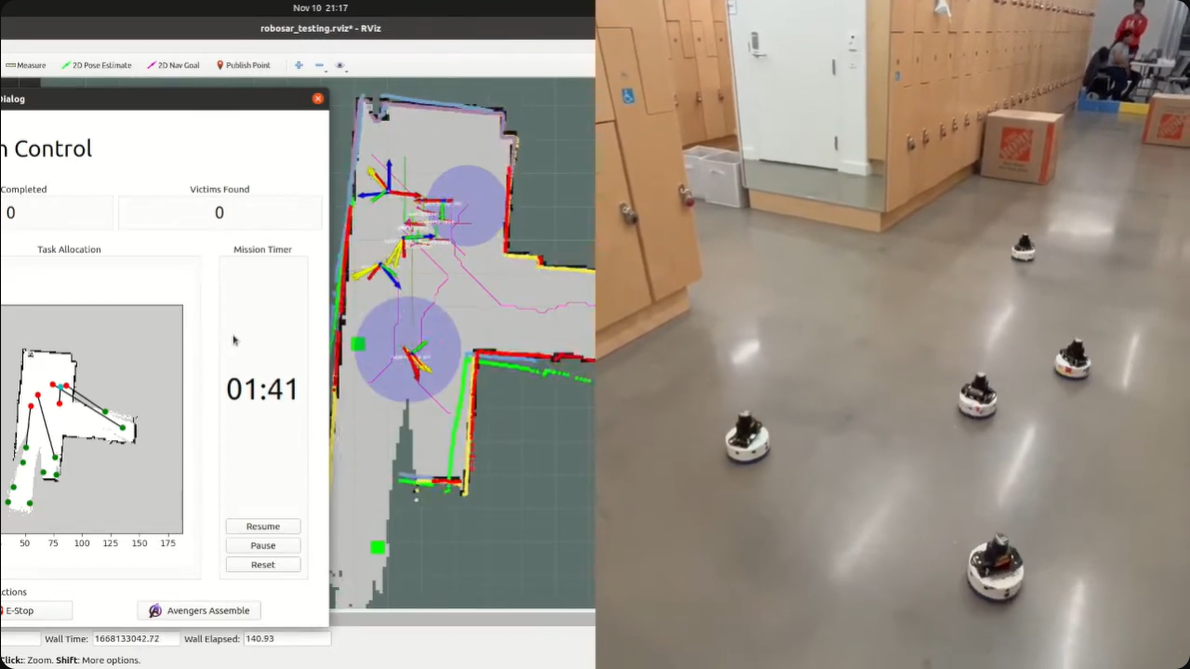
\includegraphics[width=\linewidth, height=4.5cm]{Project_motivation.png}
        \caption{Project Motivation}
        \label{fig:proj_motivation}
    \end{minipage}
    \hfill
    \begin{minipage}[t]{0.48\textwidth}
        \centering
        \includegraphics[width=\linewidth, height=4.5cm]{Victim_localization.png}
        \caption{Swarm Victim Localization Example}
        \label{fig:victim_loc}
    \end{minipage}
\end{figure}

\subsection{Spatial Parallelism and Temporal Efficiency}
In traditional SLAM, the time required to map an environment is directly proportional to the total area and the complexity of the floor plan. By utilizing a swarm, we implement spatial parallelism. The mapping task is treated as a distributed computing problem where each robot explores a unique ``frontier''. This reduces the total mission time significantly, which is a critical factor in time-sensitive scenarios like gas leak detection or post-earthquake structural assessment.

\subsection{Scalability and Modular Deployment}
One of the most compelling motivations for swarm robotics is scalability. Unlike single-robot systems, where adding capability requires a hardware overhaul, a swarm can be scaled by simply deploying additional low-cost units. This modularity allows the system to adapt to environments of varying sizes --- from a small apartment to a multi-story warehouse --- without needing to rewrite the underlying coordination algorithms. This approach inherently improves cost-effectiveness, as multiple simple robots can achieve tasks that would typically require a single, expensive, and complex robot.

\subsection{Decentralized Intelligence and Reduced Communication Overhead}
Centralized systems suffer from ``bottlenecking,'' where a single central server must process all incoming LiDAR data, leading to latency and potential crashes. Our motivation lies in leveraging decentralized coordination. By processing local maps on-board and only sharing essential ``map fragments'' or ``keyframes'' with neighbors, the swarm minimizes the bandwidth required. This makes the system viable in buildings with thick concrete walls or poor Wi-Fi signals where a central link would fail.

% Add your content here...

\section{Problem Statement}
\label{sec:problem_statement}

Despite the theoretical advantages of swarm robotics, practical implementation faces several challenges:

\begin{enumerate}
    \item \textbf{Lack of Unified Architecture:} Existing systems often use heterogeneous components that lack interoperability.
    \item \textbf{Complex Coordination:} Achieving synchronized behavior among multiple autonomous agents requires sophisticated communication and decision-making protocols.
    \item \textbf{Hardware Constraints:} Designing cost-effective, robust, and modular robot platforms remains challenging.
    \item \textbf{Navigation Complexity:} Multi-robot path planning must account for collision avoidance, traffic management, and dynamic obstacles.
\end{enumerate}

This project addresses these challenges by developing a comprehensive, unified architecture that integrates mechanical design, electrical systems, and autonomous software into a cohesive framework.

% Add your content here...

\section{Project Objectives}
\label{sec:objectives}

The primary objectives of the \textbf{AUSRA} (Autonomous Unified Swarm Robotics Architecture) project are:

\begin{enumerate}
    \item \textbf{Mechanical Design:}
    \begin{itemize}
        \item Design a unified, modular robot chassis suitable for swarm applications.
        \item Perform systematic selection of materials and actuators using decision matrices.
        \item Validate the design through stress analysis and prototyping.
    \end{itemize}
    
    \item \textbf{Electrical System:}
    \begin{itemize}
        \item Develop a robust power distribution and management system.
        \item Integrate sensors (LiDAR, IMU, encoders) for perception and localization.
        \item Design and implement low-level firmware for motor control and sensor interfacing.
    \end{itemize}
    
    \item \textbf{Autonomous Stack:}
    \begin{itemize}
        \item Implement sensor fusion for accurate localization.
        \item Develop path planning algorithms for navigation.
        \item Create a communication framework for swarm coordination.
        \item Design omnidirectional motion control for agile maneuvering.
    \end{itemize}
    
    \item \textbf{Integration and Testing:}
    \begin{itemize}
        \item Integrate all subsystems into a functional prototype.
        \item Conduct comprehensive testing and performance evaluation.
        \item Demonstrate swarm behavior with multiple robots.
    \end{itemize}
\end{enumerate}

% Add your content here...

\section{Thesis Structure}
\label{sec:thesis_structure}

This thesis is organized into seven chapters as follows:

\begin{description}
    \item[Chapter 1: Introduction] Provides an overview of the project motivation, problem statement, objectives, and thesis organization.
    
    \item[Chapter 2: Literature Review] Reviews existing swarm architectures, mechanical design precedents, and control strategies.
    
    \item[Chapter 3: Mechanical Design \& Structural Analysis] Details the design requirements, mechanical trials, actuator selection, hardware assembly, and stress analysis.
    
    \item[Chapter 4: Electrical System \& Low-Level Configuration] Covers the electrical topology, component specifications, PCB design, and firmware implementation.
    
    \item[Chapter 5: High-Level Configuration \& Autonomous Stack] Describes the system architecture, communication stack, localization, planning, and control subsystems.
    
    \item[Chapter 6: Experimental Results \& Discussion] Presents the testing methodology, experimental results, and analysis.
    
    \item[Chapter 7: Conclusion \& Future Recommendations] Summarizes the achievements and suggests directions for future work.
\end{description}

% ============================================================================
% Chapter 2: Literature Review
% ============================================================================

\chapter{Literature Review}
\label{chap:literature}

This chapter reviews the state-of-the-art in swarm robotics, examining existing architectures, mechanical design approaches, and control strategies that inform the development of the AUSRA system.

\section{Evolution of Material Handling: From AGVs to AMRs}
\label{sec:agv_vs_amr}

\begin{figure}[H]
    \centering
    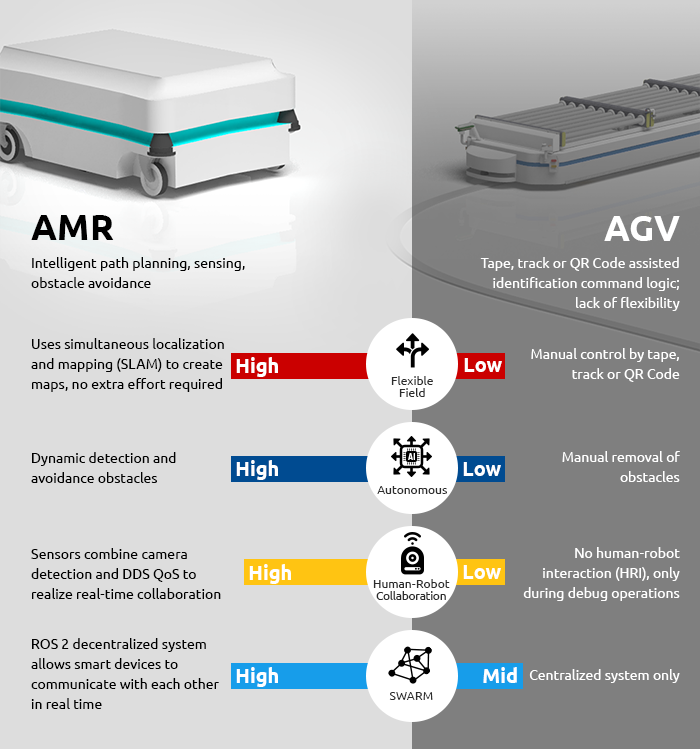
\includegraphics[width=0.6\linewidth]{figures/Chapter 2/AMRvsAGR.png}
    \caption{Evolution from AGVs to AMRs}
    \label{fig:amr_vs_agv}
\end{figure}

The coordination of mobile robots in industrial environments has evolved significantly, marked by a paradigm shift from Automated Guided Vehicles (AGVs) to Autonomous Mobile Robots (AMRs). This transition is driven by the increasing demand for flexibility and scalability in Industry 4.0 applications.

\subsection{The Limitations of AGVs}
Automated Guided Vehicles have been the standard for material transport for decades. However, they rely fundamentally on fixed infrastructure, such as magnetic tape, inductive wires, or visual markers on the floor. This dependency creates several critical limitations:
\begin{itemize}
    \item \textbf{Rigidity:} Modifying a robot's path requires physical alteration of the facility, leading to costly downtime.
    \item \textbf{Lack of Intelligence:} AGVs typically follow a "stop-and-wait" protocol when encountering obstacles. They cannot replan their path locally, which often leads to deadlocks in dynamic environments.
    \item \textbf{Installation Cost:} The need for facility modifications increases the initial deployment cost and time.
\end{itemize}

\subsection{The Superiority of AMRs}
Autonomous Mobile Robots represent the next generation of intelligent logistics. Unlike AGVs, AMRs utilize onboard sensors (Lidar, cameras) and Simultaneous Localization and Mapping (SLAM) algorithms to navigate without external infrastructure. The industry trend is heavily favoring AMRs due to their superior adaptability:
\begin{itemize}
    \item \textbf{Dynamic Navigation:} AMRs can detect obstacles and autonomously compute alternative paths in real-time, maintaining high throughput in cluttered environments.
    \item \textbf{Rapid Deployment:} A facility can be mapped digitally in hours rather than days, allowing for immediate operation.
    \item \textbf{Swarm Scalability:} New agents can be added to the fleet seamlessly by sharing the existing global map, making AMRs the ideal platform for swarm robotics research.
\end{itemize}

\begin{table}[H]
\centering
\caption{Comparative Analysis: AGV vs. AMR}
\label{tab:agv_vs_amr}
\begin{tabular}{|l|p{5cm}|p{5cm}|}
\hline
\textbf{Feature} & \textbf{Automated Guided Vehicle (AGV)} & \textbf{Autonomous Mobile Robot (AMR)} \\
\hline
\textbf{Navigation} & Physical guides (wires, tape, QR codes) & LiDAR, SLAM, Natural Features \\
\hline
\textbf{Flexibility} & Low (Requires infrastructure changes) & High (Software-defined paths) \\
\hline
\textbf{Obstacles} & Stops and waits until cleared & Navigates around dynamically \\
\hline
\textbf{Deployment} & Slow, disruptive installation & Fast, minimal facility impact \\
\hline
\textbf{Cost Model} & High initial infrastructure cost & Higher per-unit robot cost, but lower total ownership cost due to flexibility \\
\hline
\end{tabular}
\end{table}

\section{Existing Swarm Architectures}
\label{sec:swarm_architectures}

Swarm robotics has been an active research area since the early 2000s. Several notable systems and architectures have been developed:

\subsection{Kilobot}
The Kilobot platform, developed at Harvard University \cite{rubenstein2012kilobot} (Figure \ref{fig:kilobot}), is designed for large-scale swarm experiments. Key features include:
\begin{itemize}
    \item Low-cost design (approximately \$14 per unit)
    \item Infrared communication for local messaging
    \item Vibration motors for differential drive locomotion
    \item Collective charging capabilities
\end{itemize}

\subsection{e-puck}
The e-puck \cite{mondada2009puck} (Figure \ref{fig:epuck}) is a widely used educational and research platform featuring:
\begin{itemize}
    \item Differential drive with stepper motors
    \item Multiple sensor modalities (camera, IR, accelerometer)
    \item Open-source hardware and software
\end{itemize}

\subsection{Industrial Solutions}
Commercial swarm robotics systems have emerged in warehouse automation:
\begin{itemize}
    \item \textbf{Amazon Robotics (Kiva):} Grid-based navigation with centralized coordination (Figure \ref{fig:kiva})
    \item \textbf{Geek+:} Autonomous mobile robots for goods-to-person systems (Figure \ref{fig:geekplus})
    \item \textbf{Locus Robotics:} Collaborative picking robots with decentralized control (Figure \ref{fig:locus})
\end{itemize}

% Add comparison table here
\begin{table}[H]
\centering
\caption{Comparison of Existing Swarm Platforms}
\label{tab:swarm_comparison}
\begin{tabular}{|l|c|c|c|c|}
\hline
\textbf{Platform} & \textbf{Cost} & \textbf{Locomotion} & \textbf{Communication} & \textbf{Autonomy} \\
\hline
Kilobot & Very Low & Vibration & IR & Limited \\
e-puck & Medium & Differential & Bluetooth/IR & Moderate \\
Kiva & High & Differential & WiFi & High \\
AUSRA & Medium & Omnidirectional & WiFi/ROS & High \\
\hline
\end{tabular}
\end{table}

% Add detailed content here...

\begin{figure}[H]
    \centering
    % Row 1: Kilobot, E-puck, Amazon Kiva
    \begin{subfigure}[b]{0.3\textwidth}
        \centering
        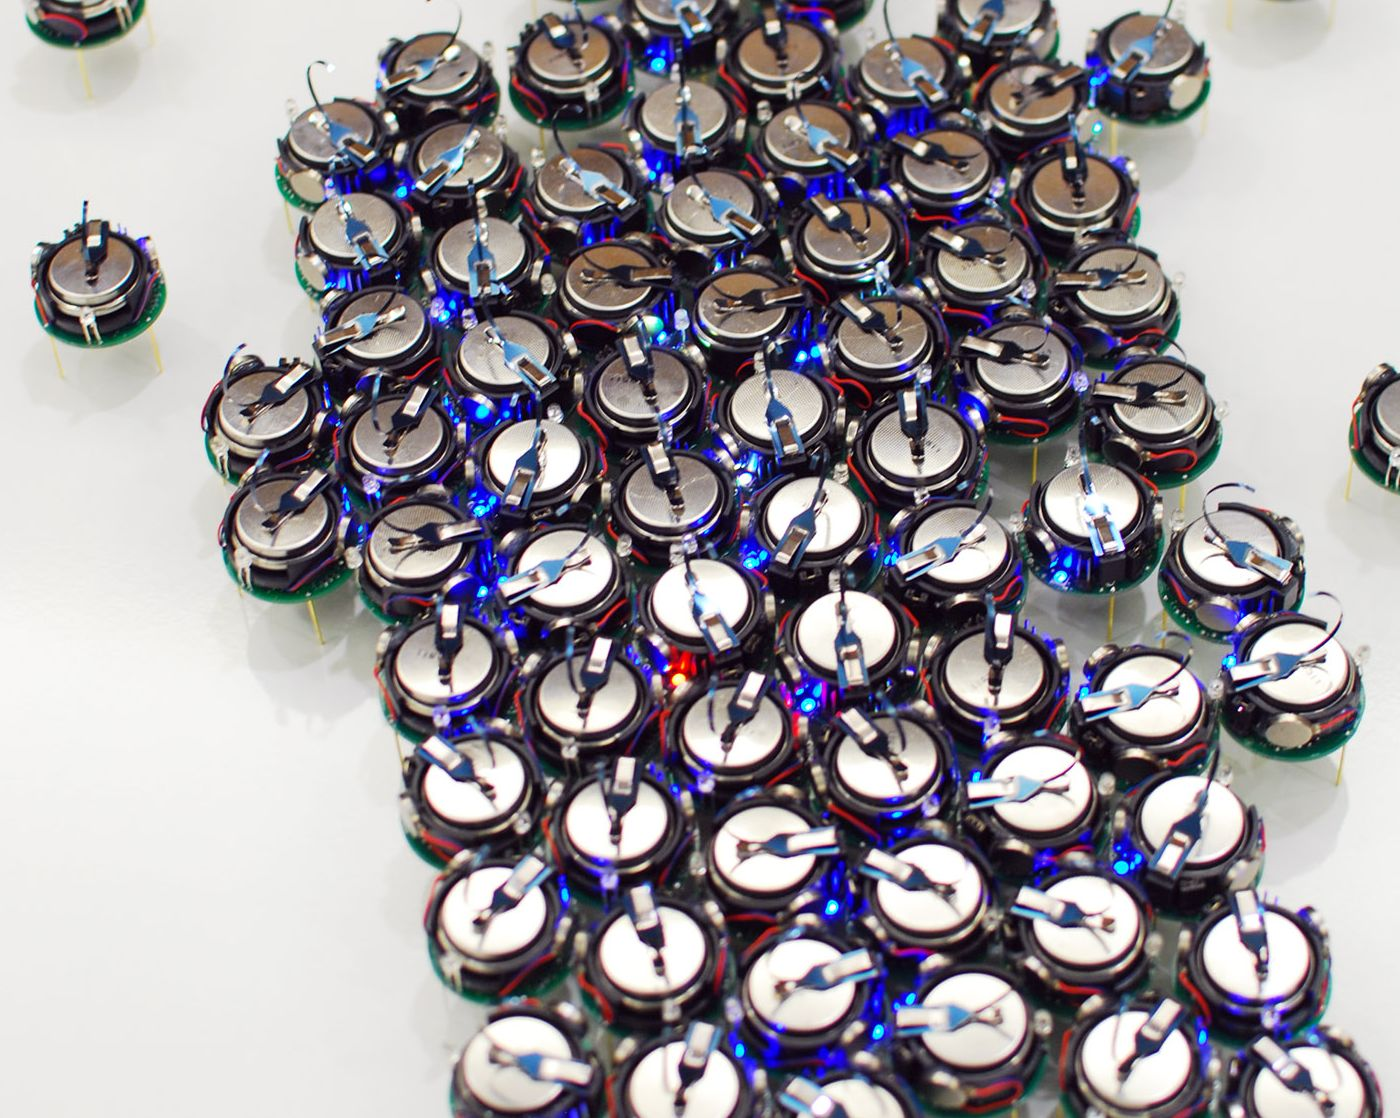
\includegraphics[width=\linewidth]{figures/Chapter 2/Kilo_bots.jpg}
        \caption{Kilobots}
        \label{fig:kilobot}
    \end{subfigure}
    \hfill
    \begin{subfigure}[b]{0.3\textwidth}
        \centering
        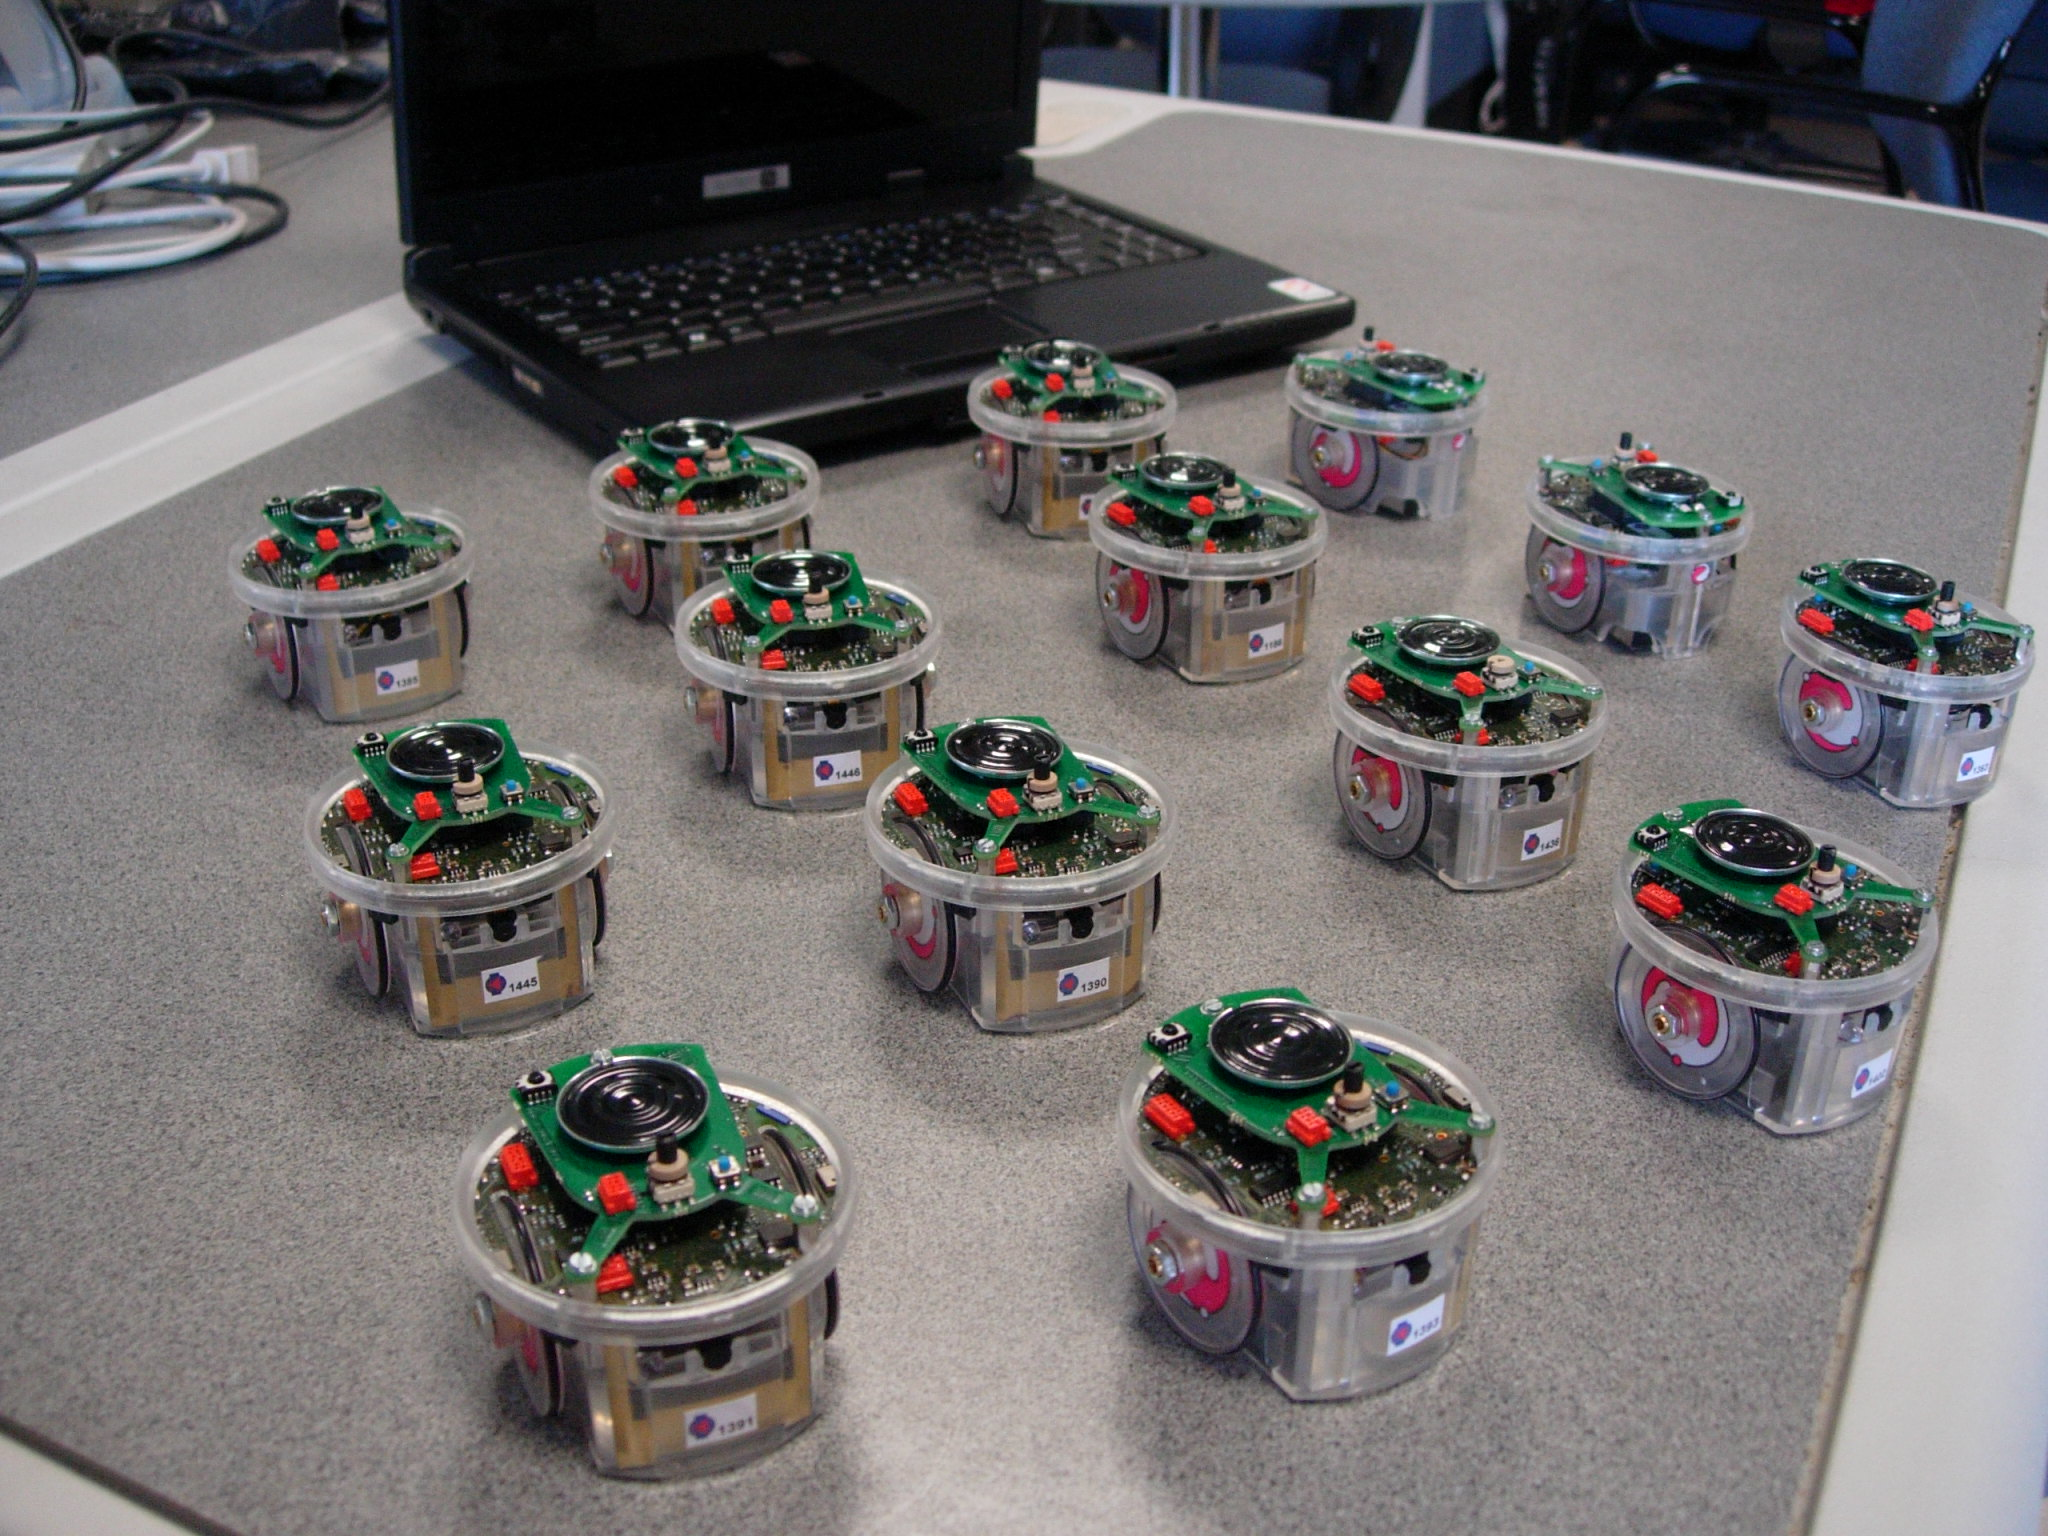
\includegraphics[width=\linewidth]{figures/Chapter 2/E-puck_robots.png}
        \caption{E-puck}
        \label{fig:epuck}
    \end{subfigure}
    \hfill
    \begin{subfigure}[b]{0.3\textwidth}
        \centering
        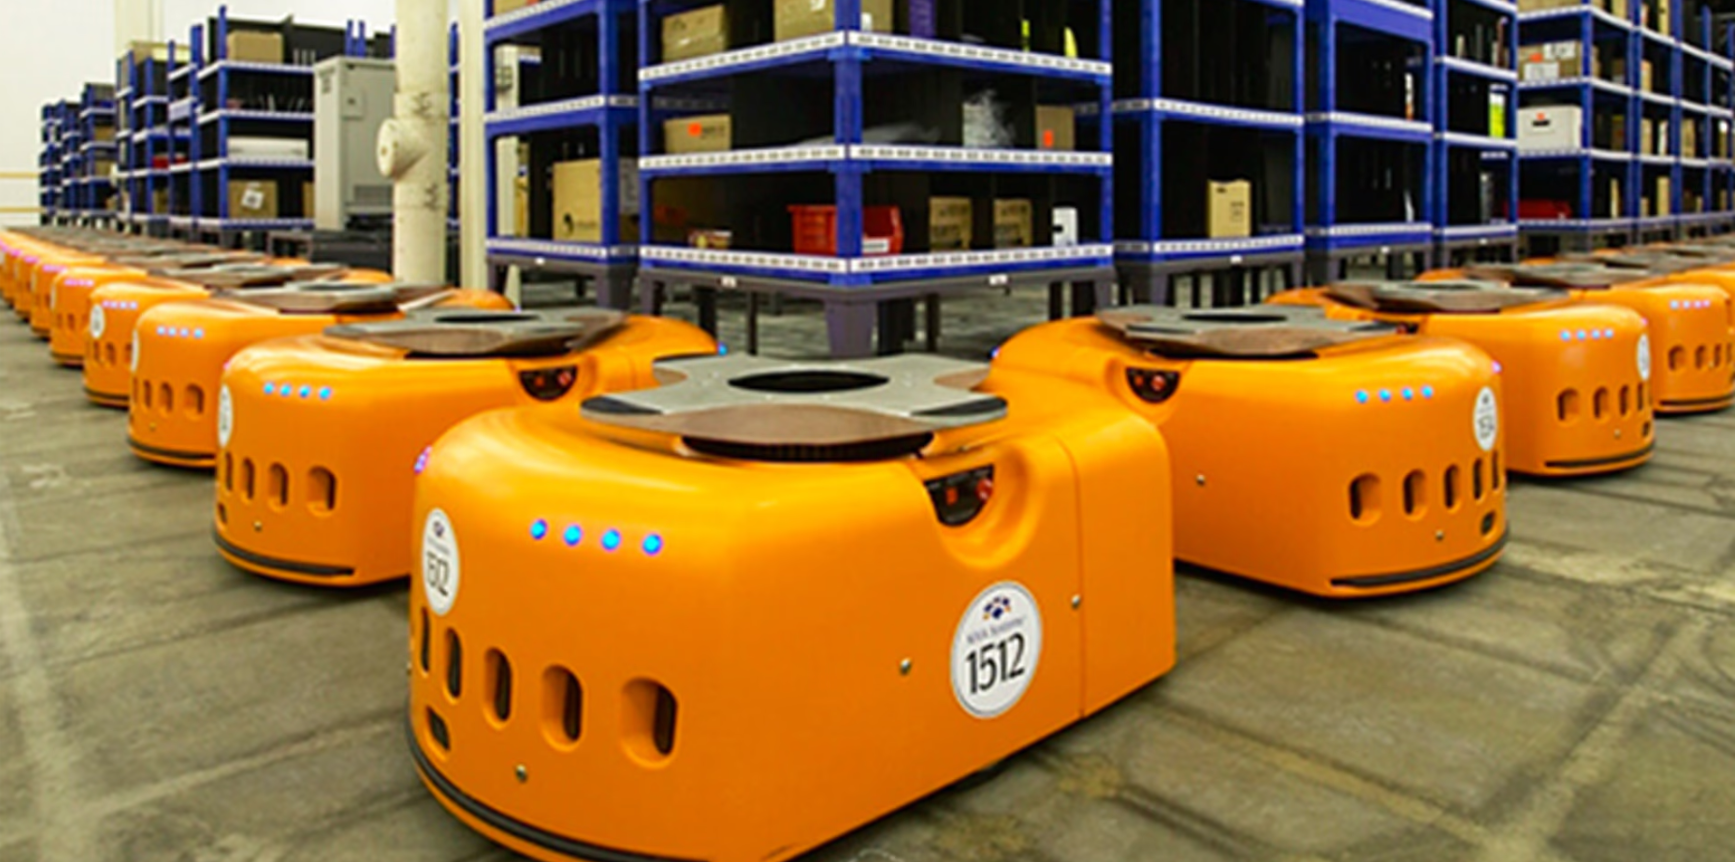
\includegraphics[width=\linewidth]{figures/Chapter 2/Amazon_kiva_robots.png}
        \caption{Amazon Kiva}
        \label{fig:kiva}
    \end{subfigure}
    
    \vspace{0.5cm}
    
    % Row 2: Geek+, Locus, AUSRA
    \begin{subfigure}[b]{0.3\textwidth}
        \centering
        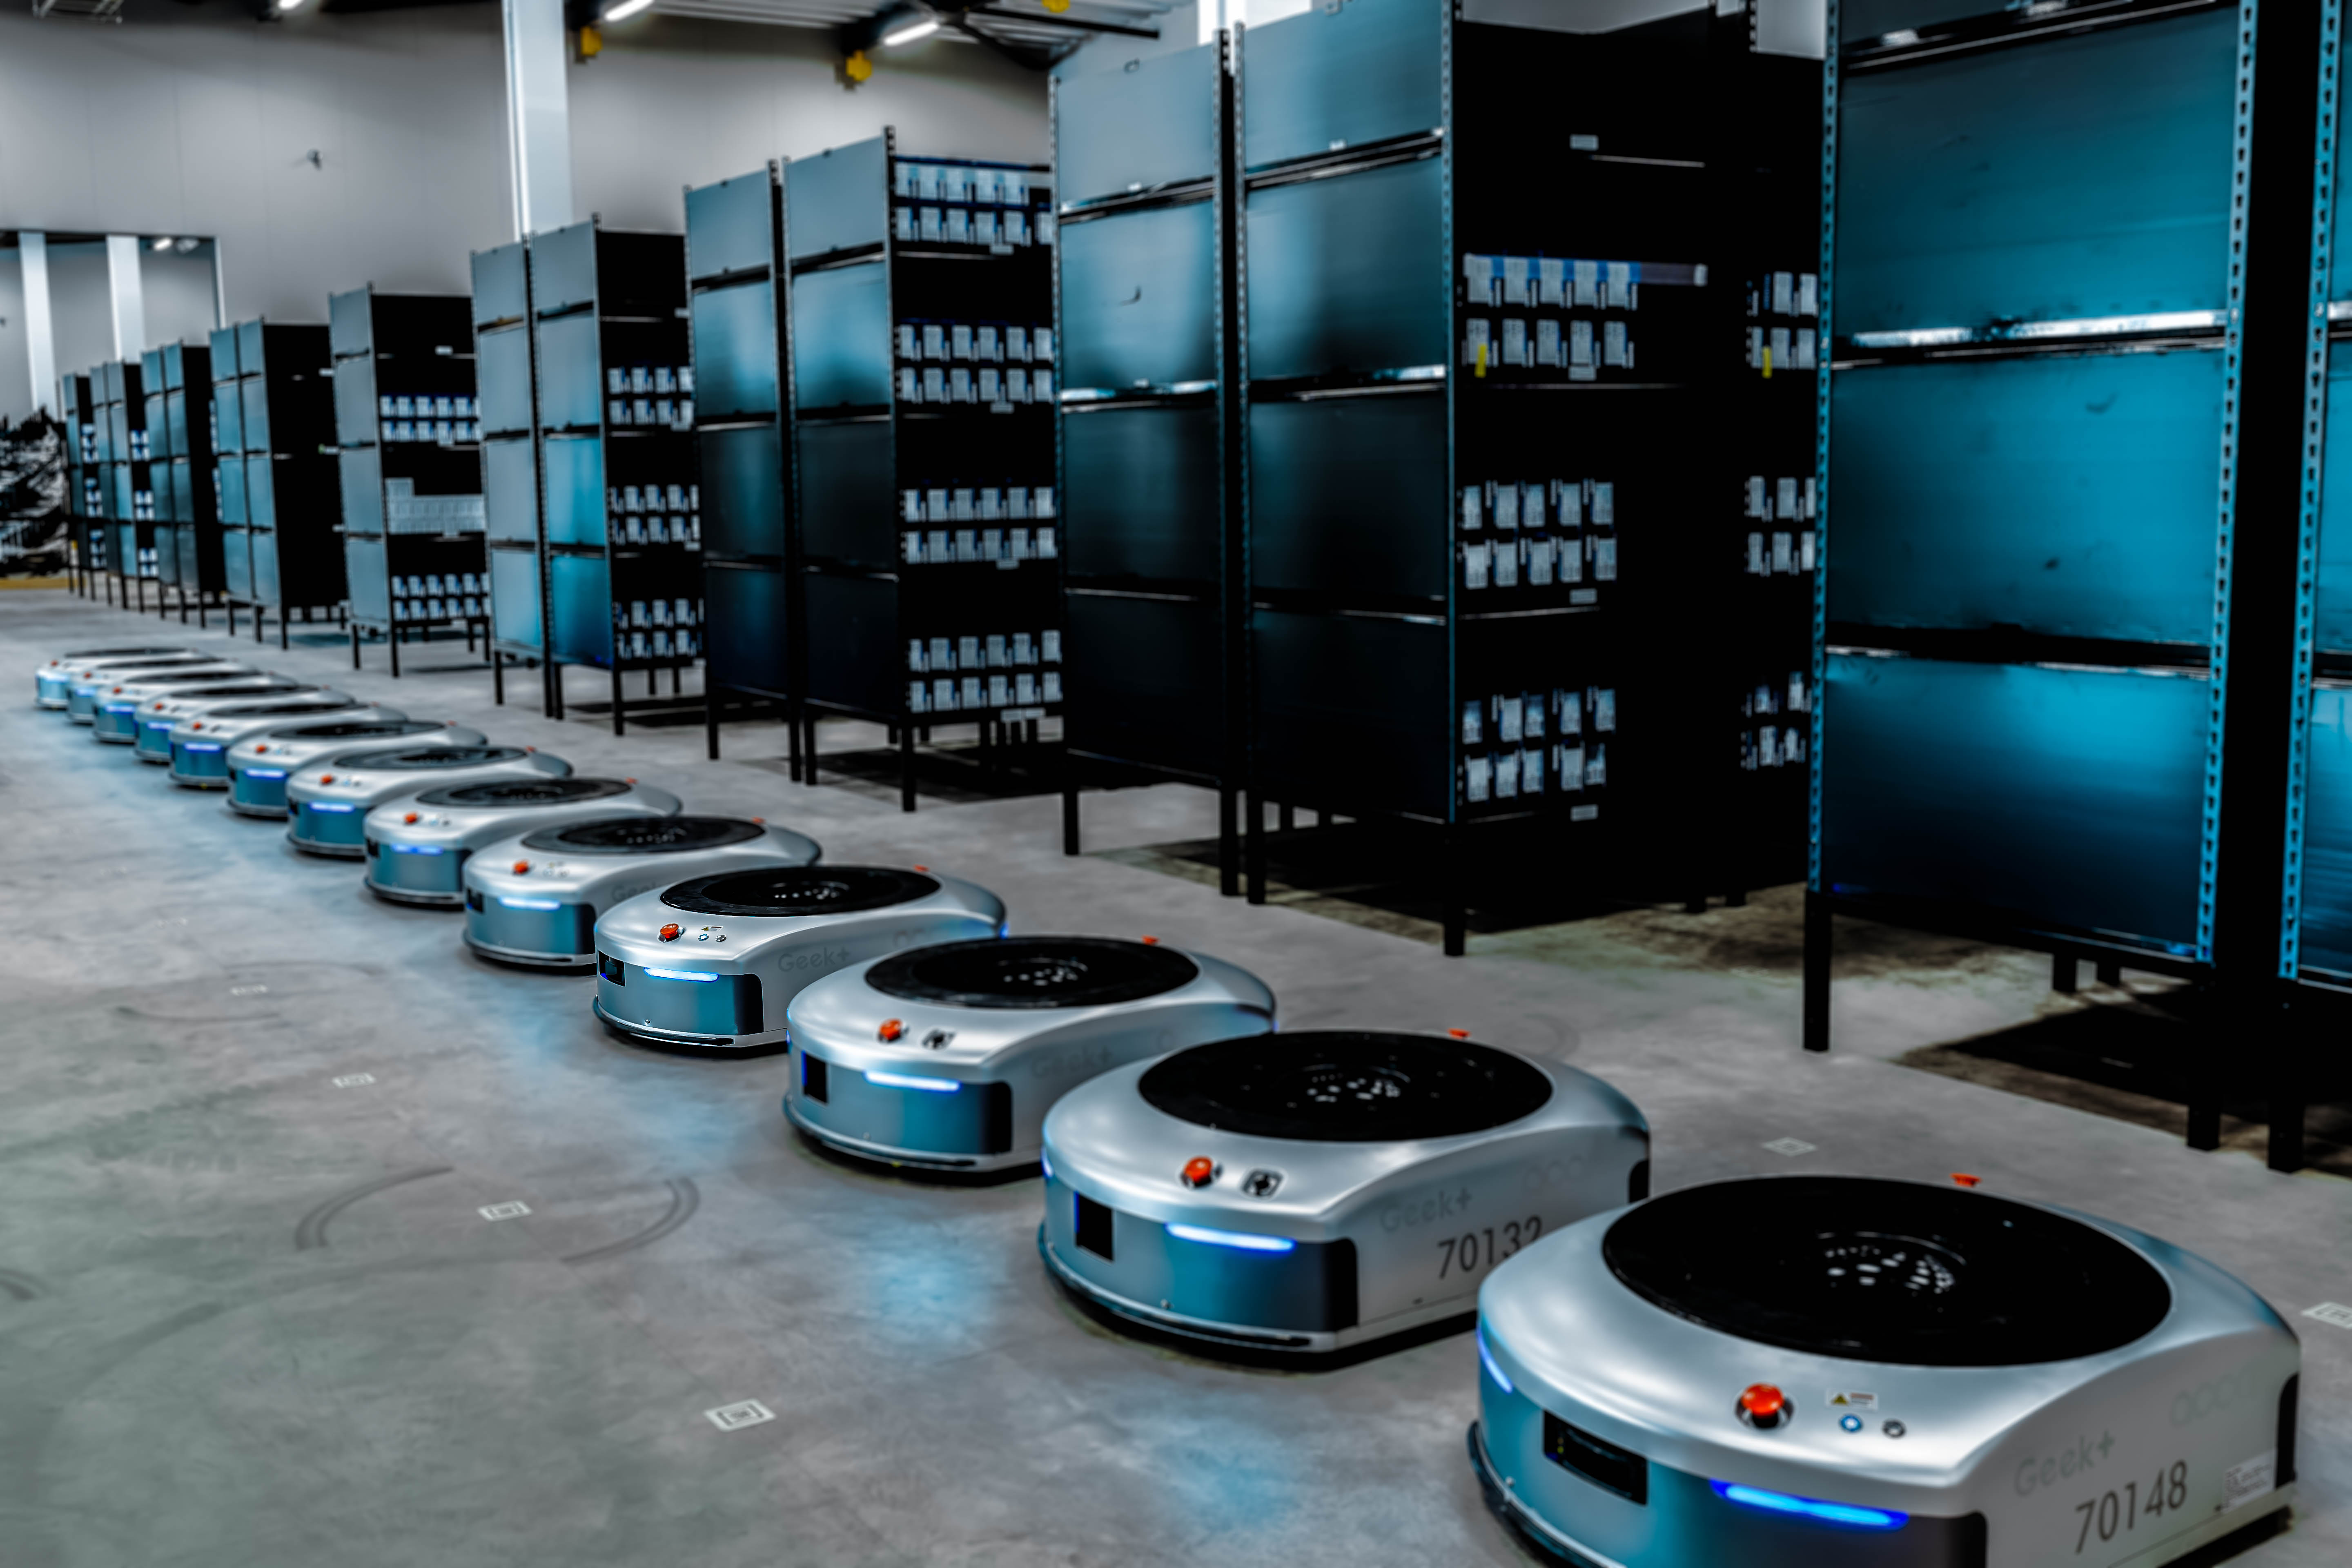
\includegraphics[width=\linewidth]{figures/Chapter 2/GeekPlus_robots.jpg}
        \caption{Geek+}
        \label{fig:geekplus}
    \end{subfigure}
    \hfill
    \begin{subfigure}[b]{0.3\textwidth}
        \centering
        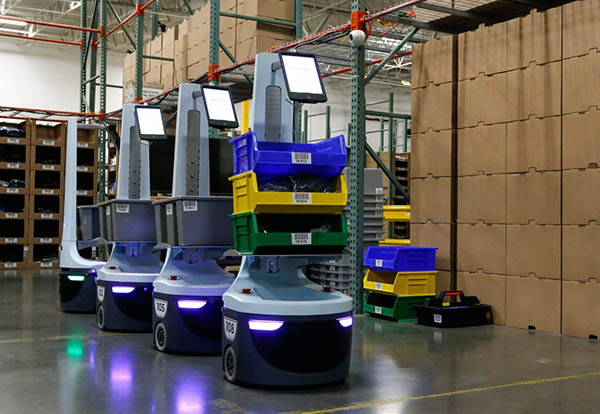
\includegraphics[width=\linewidth]{figures/Chapter 2/Locus_Bots.jpg}
        \caption{Locus Bots}
        \label{fig:locus}
    \end{subfigure}
    \hfill
    \begin{subfigure}[b]{0.3\textwidth}
        \centering
        \includegraphics[width=\linewidth]{figures/Chapter 2/Swarm_AUSRA.png}
        \caption{Our proposed AUSRA robot}
        \label{fig:ausra_proposed}
    \end{subfigure}
    
    \caption{Comparison of Existing Commercial/Research Robots and Proposed AUSRA Architecture}
    \label{fig:swarm_comparison}
\end{figure}
\newpage
\section{Mechanical Design Precedents}
\label{sec:mechanical_precedents}

\subsection{Chassis Design Approaches}
Previous research has explored various chassis configurations for mobile robots:

\begin{itemize}
    \item \textbf{Modular Designs:} Allow reconfiguration for different tasks
    \item \textbf{Monolithic Designs:} Provide structural integrity at the cost of flexibility
    \item \textbf{3D-Printed Prototypes:} Enable rapid iteration but may lack durability
\end{itemize}

\subsection{Material Selection Studies}
Material selection for mobile robot platforms typically considers:
\begin{itemize}
    \item Weight-to-strength ratio
    \item Cost and availability
    \item Manufacturability
    \item Environmental resistance
\end{itemize}

Common materials include aluminum alloys (6061-T6), ABS plastic, polycarbonate, and carbon fiber composites.

% Add your detailed content here...

\section{Control Strategies}
\label{sec:control_strategies}

\subsection{Centralized vs. Decentralized Approaches}

\textbf{Centralized Control:}
\begin{itemize}
    \item Single controller coordinates all robots
    \item Global optimization possible
    \item Single point of failure
    \item Communication bottleneck
\end{itemize}

\textbf{Decentralized Control:}
\begin{itemize}
    \item Each robot makes local decisions
    \item Scalable and robust
    \item Emergent global behavior
    \item Coordination challenges
\end{itemize}

\textbf{Hybrid Approaches:}
Modern systems often combine both paradigms:
\begin{itemize}
    \item Centralized task allocation with decentralized execution
    \item Hierarchical control structures
    \item Consensus-based decision making
\end{itemize}

\begin{figure}[H]
    \centering
    \includegraphics[width=\linewidth]{figures/Chapter 2/Centralized vs Decentralized vs Hybrid.png}
    \caption{Comparison of Control Architectures: Centralized vs. Decentralized vs. Hybrid}
    \label{fig:control_arch}
\end{figure}

\subsection{Navigation and Path Planning}
Key algorithms in multi-robot navigation include:
\begin{itemize}
    \item \textbf{A* and Dijkstra:} Global path planning
    \item \textbf{RRT/RRT*:} Sampling-based planning for complex spaces
    \item \textbf{DWA:} Dynamic Window Approach for local planning
    \item \textbf{VFH:} Vector Field Histogram for obstacle avoidance
\end{itemize}

% Add your detailed content here...

\section{Design Frameworks in Swarm Robotics}
\label{sec:design_frameworks}

Recent research has highlighted the need for structured frameworks to understand the complexity of designing robot swarms across different scales and contexts. Garzón Ramos \cite{garzonramos2024designing} proposes a three-level framework adapted from organizational theory that categorizes swarm design challenges as puzzles, problems, and the mess.

\subsection{The Puzzle: Understanding Self-Organization}
\label{subsec:puzzle}

At the foundational level, swarm robotics research has focused on \textbf{puzzles} --- well-defined scenarios where all information is available, the problem can be isolated, and repeatable solutions exist. Classic examples include:

\begin{itemize}
    \item \textbf{Aggregation:} Discovering rules that make robots cluster together
    \item \textbf{Flocking:} Identifying coordination mechanisms for collective motion
    \item \textbf{Pattern Formation:} Determining control laws for specific geometric arrangements
\end{itemize}

These studies establish the fundamental principles of self-organization and emergence in multi-robot systems. Once the underlying rules are discovered, they become generalizable primitives that can be reproduced across different platforms.

\subsection{The Problem: Task-Oriented Design with Trade-offs}
\label{subsec:problem}

As the field matures into an engineering discipline, the focus shifts to \textbf{problems} --- scenarios introducing uncertainty and multiple solutions with different trade-offs. At this level:

\begin{itemize}
    \item \textbf{Performance Metrics:} Designers must define what constitutes successful behavior
    \item \textbf{Automatic Design:} Optimization and machine learning methods combine self-organization primitives to achieve specific task objectives
    \item \textbf{Behavior Composition:} Finite state machines or behavior trees orchestrate different collective behaviors across mission phases
\end{itemize}

The AUSRA system operates primarily at this level, leveraging known principles of swarm coordination while optimizing for warehouse automation tasks. The architecture combines multiple behavioral primitives (navigation, collision avoidance, task allocation) with performance-driven tuning.

\subsection{The Mess: Real-World Deployment Complexity}
\label{subsec:mess}

The highest level of complexity represents \textbf{the mess} --- systems operating in real-world environments with:

\begin{itemize}
    \item \textbf{Human Interaction:} Workers, customers, and operators sharing the workspace
    \item \textbf{Uncontrolled Variables:} Dynamic obstacles, changing lighting, network disruptions
    \item \textbf{Interdependent Systems:} Integration with existing infrastructure and workflows
    \item \textbf{Context Awareness:} Understanding situational requirements beyond pre-programmed behaviors
\end{itemize}

Embracing "the mess" requires acknowledging that not all variables can be controlled or optimized. Future swarm systems must develop adaptive capabilities, robust failure modes, and intuitive human interfaces to operate reliably in these complex scenarios.

\subsection{Stigmergy as an Interface Mechanism}
\label{subsec:stigmergy}

\textbf{Stigmergy} --- communication through environmental modification --- offers a promising approach for bridging human-swarm interaction, particularly in manufacturing and logistics contexts \cite{garzonramos2024designing}. Unlike explicit digital communication, stigmergy allows:

\begin{itemize}
    \item \textbf{Implicit Coordination:} Objects placed in specific locations signal intent to nearby robots
    \item \textbf{Low-Bandwidth Interaction:} No need for Wi-Fi connectivity or complex user interfaces
    \item \textbf{Organic Integration:} Humans and robots share the same physical workspace naturally
\end{itemize}

For example, a worker placing a component in a designated area triggers robot pickup and transport without explicit commands. The environment itself becomes the communication medium, reducing cognitive load and system complexity.

\subsection{AUSRA's Position in the Framework}
\label{subsec:ausra_framework}

The AUSRA project addresses challenges at the \textbf{problem} level:
\begin{itemize}
    \item Combining navigation, localization, and coordination primitives
    \item Optimizing for task performance in structured warehouse environments
    \item Providing a modular architecture for different operational scenarios
\end{itemize}

While acknowledging the complexity of \textbf{the mess} as future work, AUSRA establishes a foundation for transitioning swarm research from controlled experiments to practical applications.



\section{Multi-Robot Exploration and Mapping}
\label{sec:mr_slam}

A critical component of collaborative swarm systems is the ability to enable multiple robots to simultaneously map an unknown environment and localize themselves within it. This problem, known as Multi-Robot SLAM (MR-SLAM), extends the traditional Simultaneous Localization and Mapping (SLAM) problem to distributed systems.

\subsection{Collaborative Mapping Approaches}
Early work by Simmons et al. \cite{simmons2000coordination} and Burgard et al. \cite{burgard2005coordinated} demonstrated that coordinating the exploration targets of multiple robots significantly reduces the time required to map a given area. The "frontier-based exploration" strategy proposed by Yamauchi \cite{yamauchi1997frontier} remains a foundational concept, where robots are directed to the boundaries between open space and unexplored territory.

More recently, sampling-based methods such as Rapidly-exploring Random Trees (RRTs) have been adapted for autonomous multi-robot exploration \cite{umari2017autonomous}, enabling efficient coverage of complex, cluttered environments.

\subsection{Greedy Frontier Exploration: \texttt{explore\_lite}}
\label{subsec:explore_lite}
A practical and widely-adopted realization of Yamauchi's frontier strategy is the open-source \texttt{explore\_lite} package from the \texttt{m-explore} stack \cite{hornerexplore}. Rather than maintaining an explicit map representation of its own, \texttt{explore\_lite} operates directly on the occupancy grid published by the navigation costmap, making it lightweight and straightforward to integrate with a Nav2-based stack. The node continuously detects frontiers --- contiguous boundaries between free and unknown cells --- and selects the next goal by ranking candidate frontiers with a weighted cost function that trades off the distance to a frontier against its size (information gain) and the robot's current heading. The selected frontier centroid is then dispatched as a navigation goal, and the cycle repeats until no frontiers remain, at which point the environment is considered fully explored.

The AUSRA system adopts \texttt{explore\_lite} as its single-robot exploration driver. Its frontier-ranking weights and detection thresholds were tuned for the cluttered indoor environments characteristic of search-and-rescue scenarios: the minimum frontier size was lowered so that narrow passages are not missed, the gain term was increased to favour expanding the mapped area, and the potential (distance) term was balanced to produce smoother transitions between successive frontiers rather than erratic back-and-forth motion. The specific parameter values and the tuning rationale are detailed in Chapter~\ref{chap:hardware}.

\subsection{Pose Graph Optimization}
Collaborative mapping often relies on a shared "Pose Graph" to maintain consistency across the swarm's global map. In this framework, each robot's trajectory is represented as a series of nodes (poses) connected by constraints derived from odometry and sensor measurements. A key challenge in MR-SLAM is "loop closure" --- recognizing when a robot has returned to a previously visited location or crossed paths with another robot. When a loop closure is detected, the entire graph is optimized to minimize error accumulation. Tools like SLAM Toolbox \cite{macenski2021slam} provide robust implementations of pose graph optimization that can be adapted for multi-robot scenarios, as demonstrated in the RoboSAR project.

\subsection{Multi-Robot Map Merging}
\label{subsec:map_merging}
Whereas pose graph optimization fuses observations \emph{within} a single robot's trajectory, a swarm tasked with collaboratively mapping an environment must additionally combine the individual occupancy grids produced by each agent into a single, globally consistent map. This fusion problem --- map merging --- can be approached in two fundamentally different ways.

The first approach, \textbf{feature-based merging}, makes no assumption about where the robots started. Instead, it treats each robot's map as an image and searches for the rigid transformation (rotation and translation) that best aligns overlapping structure, typically by extracting and matching visual features between the grids. This is robust to unknown starting configurations but depends on the maps sharing enough overlapping, distinctive geometry for a confident match, and it can fail or produce misaligned results in featureless or highly symmetric spaces.

The second approach, \textbf{merging from known initial poses}, assumes the relative spawn positions of the robots are known in advance. Each map can then be transformed directly into a common world frame using the known offsets, sidestepping the feature-matching step entirely and guaranteeing a deterministic, correctly-scaled merge. The trade-off is the operational requirement that robots be deployed from surveyed or otherwise known starting points.

The open-source \texttt{multirobot\_map\_merge} package, also part of the \texttt{m-explore} stack \cite{hornerexplore}, implements both strategies and is selectable at runtime via a single parameter. The AUSRA system adopts the \textbf{known-initial-pose} strategy: in a coordinated search-and-rescue deployment the robots are launched from a known formation, so their relative offsets are available and a deterministic merge is preferable to the uncertainty of feature matching on the sparse grids typical of partially-explored disaster environments. The concrete realization of this strategy on the AUSRA hardware --- including how each robot's spawn offset is incorporated and how the per-robot maps are aggregated into a shared global map --- is presented in Chapter~\ref{chap:swarm}.

\section{Task Allocation in Swarms}
\label{sec:task_allocation}

Efficiently assigning tasks to individual robots is essential for maximizing the performance of a swarm. Korsah et al. \cite{korsah2013comprehensive} provide a comprehensive taxonomy for Multi-Robot Task Allocation (MRTA), categorizing problems based on:
\begin{itemize}
    \item \textbf{Single-Task vs. Multi-Task Robots (ST/MT):} Whether a robot can perform one or multiple tasks at a time.
    \item \textbf{Single-Robot vs. Multi-Robot Tasks (SR/MR):} Whether a task requires one or multiple robots to complete.
    \item \textbf{Instantaneous vs. Time-Extended Assignment (IA/TA):} Whether tasks are assigned immediately or planned over a future horizon.
\end{itemize}

\begin{figure}[H]
    \centering
    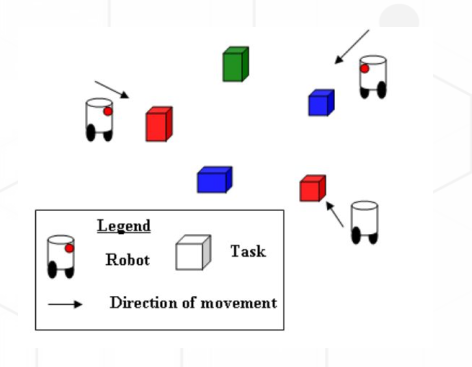
\includegraphics[width=0.6\linewidth]{figures/Chapter 2/Task_allocation.png}
    \caption{Taxonomy of Multi-Robot Task Allocation (MRTA)}
    \label{fig:task_allocation}
\end{figure}

For Search and Rescue (SAR) applications, Queralta et al. \cite{queralta2020collaborative} highlight the importance of dynamic task allocation mechanisms that can adapt to the changing state of the environment and the swarm, such as the discovery of a victim or the failure of a robot agent.

\section{Summary}
\label{sec:lit_summary}

This literature review has identified key considerations for the AUSRA system:
\begin{enumerate}
    \item A hybrid control architecture balances scalability and coordination
    \item Omnidirectional locomotion offers superior maneuverability for swarm operations
    \item Modular mechanical design enables flexibility and maintainability
    \item ROS provides a robust framework for autonomous navigation
\end{enumerate}

The following chapters detail how these insights informed the design and implementation of the AUSRA system.

% ============================================================================
% Chapter 3: Hardware Selection & Mechanical Design
% ============================================================================

\chapter{Hardware Selection \& Mechanical Design of Ausrabot}
\label{chap:mechanical}

\section{Introduction to the Hardware Architecture}
\label{sec:hardware_intro}

The hardware architecture of the Ausra swarm is designed to bridge the gap between physical robustness and high-level autonomous intelligence \cite{siegwart2011introduction}. To achieve collaborative 2D mapping, the mechanical structure must serve as a stable, mobile platform for sensitive electronic sensors while maintaining the agility required for swarm formations.

\subsection{Design Requirements and Constraints}
In the context of collaborative 2D mapping, the mechanical structure must serve as a stable, mobile platform for sensitive electronic sensors. The following requirements were established to ensure the swarm can navigate indoor environments efficiently.

\begin{table}[H]
    \centering
    \caption{Robot Design Requirements}
    \label{tab:design_reqs}
    \begin{tabular}{|l|l|}
    \hline
    \textbf{Requirements} & \textbf{Value/Description} \\
    \hline
    Maximum Weight for the Robot & 5 Kg \\
    \hline
    Minimum Velocity for the Robot & 0.2 m/s \\
    \hline
    Compactness & \begin{tabular}{@{}l@{}}Max Length: 30 cm \\ Max Height: 20 cm\end{tabular} \\
    \hline
    Modularity and Serviceability & Stackable Layers \\
    \hline
    \end{tabular}
\end{table}

\subsubsection{Maximum Weight of The Robot}
\begin{itemize}
    \item \textbf{Power Efficiency:} A lighter chassis reduces the torque required from the motors, thereby extending battery life for longer mapping missions.
    \item \textbf{Manufacturing Materials and Costs:} Meeting the 5-kilogram weight limit involves careful selection of materials during the manufacturing process. The choice of lightweight yet durable materials can impact not only the robot’s weight but also manufacturing costs. Balancing these factors is essential for achieving an optimal design.
\end{itemize}

\subsubsection{Minimum Velocity of the Robot}
To ensure the swarm covers the building floor plan in reasonable timeframe, a minimum velocity of 0.2 m/s was established.
\begin{itemize}
    \item \textbf{SLAM Data Consistency:} While higher speeds might seem better, mapping sensors (like LiDAR) require a steady movement to prevent "motion blur" in the point cloud. A velocity of 0.2 m/s provides a balanced trade-off between exploration speed and the sampling density required for high-resolution 2D maps.
    \item \textbf{Controllability:} This speed allows the PID controllers to maintain smooth trajectories even when the robot encounters minor floor irregularities or transitions.
\end{itemize}

\subsubsection{Spatial Constraints (Compactness)}
The physical dimensions are restricted to a Maximum length of 30 cm and a Maximum height of 20 cm. This ensures the robot can navigate human-centric environments:
\begin{itemize}
    \item \textbf{Aperture Navigation:} A 30 cm width allows the robot to easily pass through standard doorways and navigate between furniture legs or narrow office corridors.
    \item \textbf{Low profile:} The 20 cm height constrain ensures a low center of gravity. Furthermore, it allows the robot to map under certain obstacles (like tables or benches) where a taller robot might be considered.
    \item \textbf{Portability:} Compact robots are easier to transport to the deployment site in batches, which is a core requirement for any multi-robot deployment.
\end{itemize}

\subsubsection{Modularity and Serviceability}
\begin{itemize}
    \item \textbf{Rapid Repair:} The internal components (sensors, microcontroller, and motor drivers) are organized in a "stack" system. This gives us the ability to replace a faulty sensor or damaged component and make it easy for charging the battery without dismantling the entire chassis.
    \item \textbf{Standardization:} Using standardized fasteners and mounting patterns across all robots in the swarm ensures that parts are interchangeable.
\end{itemize}

\subsection{Functional Layer Decomposition}
To manage the complexity of the swarm's tasks, the Ausra robot’s hardware architecture is physically and logically split into three functional layers. This modularity ensures that high-level computing tasks do not interfere with time-critical motor control.
\begin{enumerate}
    \item \textbf{Locomotion \& Actuation Layer (The Base):} This bottom layer houses the physical chassis, Omni-wheels, motor drivers, and DC motors. Its sole purpose is to transform electrical energy into precise physical displacement.
    \item \textbf{Low-Level Control \& Interface Layer (The Nervous System):} Centered around the ESP32, this middle layer handles real-time tasks: reading encoders and executing PID loops. It acts as the bridge between the high-level brain and the motors.
    \item \textbf{Perception \& High-Level Computing Layer (The Brain):} This top layer houses the high-level processor, the depth camera and Lidar. It handles the most computationally expensive tasks, such as Spatial AI, obstacle avoidance, and SLAM mapping.
\end{enumerate}

\section{Robot's Hardware Selection}
\label{sec:hardware_selection}

After defining the main requirements and the hardware architecture, this section would demonstrate how we selected all hardware components for our robot starting from the selection of wheels for maneuverability of the swarm robots moving together to the high-level board for the autonomous tasks execution.

\subsection{Locomotion \& Actuation Group}
The locomotion and actuation group constitutes the physical "base" layer of the Sirius robot. This group is responsible for translating digital control signals into precise mechanical movement \cite{corke2017robotics}. To meet the requirements of holonomic motion and a 5kg weight limit, the following components were selected through a series of trade-off analyses.

\subsubsection{Locomotion System (Robot's wheel selection)}
The locomotion system is the most fundamental mechanical decision for the Ausra swarm robots. For a swarm to exhibit collective intelligence, individual units must possess high maneuverability to execute synchronized patterns without colliding \cite{bayer2019omnidirectional}. This section explores the diverse wheel technologies available in robotics and evaluates their suitability for the project.

\paragraph{A. Exploration of Robotic Wheel Technologies}
Before selecting the drive system, four primary locomotion categories were analyzed based on their mechanical architecture and typical industrial applications (see Figure \ref{fig:wheel_technologies}):

\begin{itemize}
    \item \textbf{Standard Fixed Wheels (Differential Drive) (Figure \ref{fig:wheel_technologies}a):}
    \begin{itemize}
        \item \textbf{Description:} These are conventional wheels, typically with rubber or polyurethane treads, fixed to a single axis of rotation.
        \item \textbf{Typical Applications:} Used in most commercial vacuum robots (like Roomba), warehouse AGVs, and high-speed transport vehicles.
        \item \textbf{Mechanical Behavior:} They offer excellent traction and high load capacity. However, they are non-holonomic; to move sideways, the robot must first rotate its entire body, making path planning in tight spaces more complex.
        \item \textbf{Pros:} High traction, high efficiency, and simple control logic.
        \item \textbf{Cons:} Non-holonomic; requires turning radius to change direction, limiting maneuverability in tight swarm formations.
    \end{itemize}

    \item \textbf{Mecanum Wheels (Figure \ref{fig:wheel_technologies}b):}
    \begin{itemize}
        \item \textbf{Description:} A specialized wheel with integrated rollers mounted at a 45\degree\ angle around its circumference.
        \item \textbf{Typical Applications:} Heavy-duty industrial platforms and high-end research robots (like the KUKA youBot).
        \item \textbf{Mechanical Behavior:} By varying the speed and direction of four independent Mecanum wheels, a robot can move in any direction (holonomic). However, they require a 4-wheel rectangular setup to work effectively, which increases weight and control complexity.
        \item \textbf{Pros:} Full holonomic movement in any orientation.
        \item \textbf{Cons:} Requires a 4-wheel rectangular chassis (increasing weight/cost) and experiences high vibration due to the diagonal roller orientation.
    \end{itemize}

    \item \textbf{Omni-Directional Wheels (Omni-Wheels) (Figure \ref{fig:wheel_technologies}c):}
    \begin{itemize}
        \item \textbf{Description:} Similar to Mecanum wheels, but the peripheral rollers are mounted at 90\degree\ (perpendicular) to the main wheel’s axis.
        \item \textbf{Typical Applications:} Robot soccer (RoboCup), educational platforms, and small-scale swarm robotics.
        \item \textbf{Mechanical Behavior:} These wheels roll forward like standard wheels but can slide laterally with near-zero friction. They are unique because they allow for a 3-wheel 120\degree\ configuration, which provides full 3-DOF movement with the fewest possible motors.
        \item \textbf{Pros:} Allows for 3-DOF holonomic movement, facilitates compact 3-wheel layouts, and offers smooth motion on flat surfaces.
        \item \textbf{Cons:} Lower traction compared to rubber wheels; limited to relatively flat, indoor environments.
    \end{itemize}
\end{itemize}

\begin{figure}[H]
    \centering
    \begin{subfigure}[b]{0.32\textwidth}
        \centering
        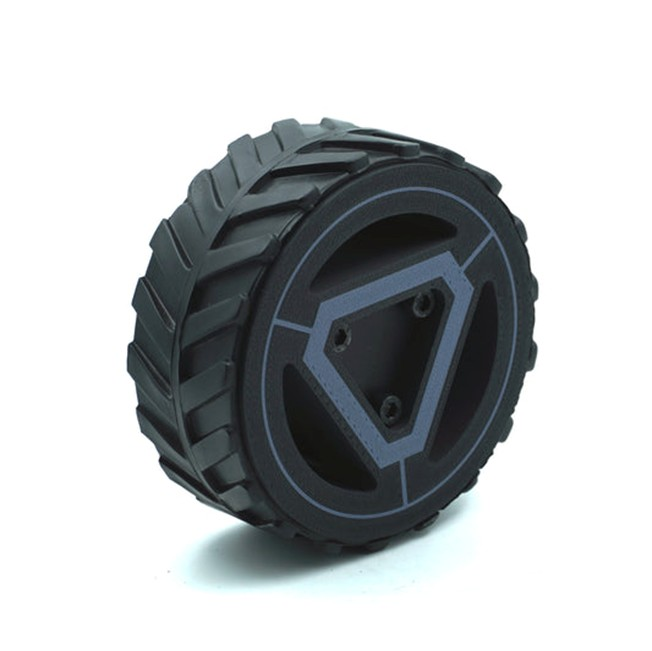
\includegraphics[height=3.5cm, keepaspectratio]{figures/Chapter 3/Standard_Fixed_wheels.jpg}
        \caption{Standard Fixed Wheels}
        \label{fig:fixed_wheels}
    \end{subfigure}
    \hfill
    \begin{subfigure}[b]{0.32\textwidth}
        \centering
        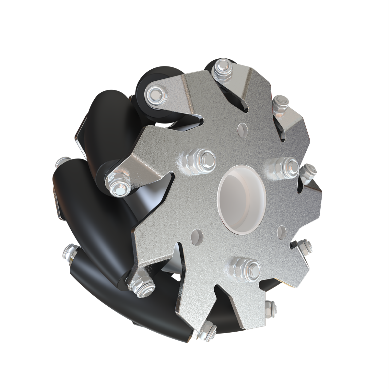
\includegraphics[height=3.5cm, keepaspectratio]{figures/Chapter 3/mecanum_wheel.png}
        \caption{Mecanum Wheel}
        \label{fig:mecanum_wheel}
    \end{subfigure}
    \hfill
    \begin{subfigure}[b]{0.32\textwidth}
        \centering
        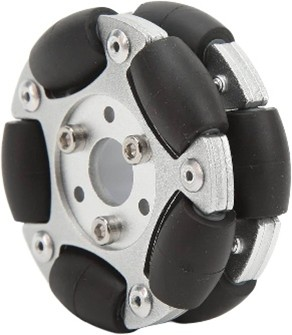
\includegraphics[height=3.5cm, keepaspectratio]{figures/Chapter 3/omnidirectional_wheel.jpg}
        \caption{Omni-Directional Wheel}
        \label{fig:omni_wheel}
    \end{subfigure}
    \caption{Robotic Wheel Technologies Comparison}
    \label{fig:wheel_technologies}
\end{figure}

\paragraph{B. Selection Criteria}
To determine the optimal wheel for our robots, seven specific criteria were established to evaluate the wheel types against the "Ausra" project requirements:
\begin{enumerate}
    \item \textbf{Holonomic Motion:} The ability to move in any direction instantly without changing the robot's heading. This is crucial for executing synchronized swarm formations.
    \item \textbf{Environment Compatibility:} Performance on flat, indoor laboratory surfaces.
    \item \textbf{Control Simplicity:} The mathematical ease of mapping desired robot velocities ($V_x, V_y, \omega$) to motor PWM signals using the ESP32.
    \item \textbf{Traction:} The grip of the wheel on the surface to prevent drifting and ensure accurate odometry feedback.
    \item \textbf{Space/Weight:} Keeping the physical footprint small to allow multiple robots to navigate tight spaces simultaneously.
    \item \textbf{Number of Wheels Needed:} This affects the complexity of the assembly and the total number of motors and motor drivers required per robot.
    \item \textbf{Unit Cost:} The financial impact of the wheel choice, which scales significantly across a swarm of three or more robots.
\end{enumerate}

\paragraph{C. Quantitative Selection Matrix}
The following selection matrix is conducted to rank each locomotion type and provide a final selection for our Ausra robots wheels for the desired motion and performance:

\begin{table}[H]
\centering
\caption{Wheel Selection Matrix}
\label{tab:wheel_matrix}
\resizebox{\textwidth}{!}{%
\begin{tabular}{|l|c|c|c|c|c|c|c|}
\hline
\multirow{2}{*}{\textbf{Criteria}} & \multirow{2}{*}{\textbf{Weights}} & \multicolumn{2}{c|}{\textbf{Standard fixed}} & \multicolumn{2}{c|}{\textbf{Mecanum}} & \multicolumn{2}{c|}{\textbf{Omni}} \\ \cline{3-8} 
 &  & Rating/5 & Score & Rating/5 & Score & Rating/5 & Score \\ \hline
Holonomic motion & 5 & 1 & 5 & 5 & 25 & 5 & 25 \\ \hline
Unit cost & 4 & 5 & 20 & 3 & 12 & 4 & 16 \\ \hline
No. of wheels & 4 & 3 & 12 & 2 & 8 & 3 & 12 \\ \hline
Env. Compatibility & 3 & 4 & 12 & 5 & 15 & 5 & 15 \\ \hline
Control Simplicity & 3 & 5 & 15 & 3 & 9 & 4 & 12 \\ \hline
Traction & 3 & 4 & 12 & 3 & 9 & 3 & 9 \\ \hline
Space/weight & 2 & 5 & 10 & 3 & 6 & 4 & 8 \\ \hline
\textbf{Final Scores} &  &  & \textbf{84} &  & \textbf{84} &  & \textbf{97} \\ \hline
\end{tabular}%
}
\end{table}

\paragraph{D. Selection Rationale}
The Omni-wheel emerged as the superior choice for the "Ausra" project with a weighted score of 97. The selection is justified by the following engineering trade-offs:
\begin{itemize}
    \item \textbf{Indoor Optimization:} As the swarm is designed for indoor buildings and laboratories, the Omni-wheel's ability to "slide" laterally on flat floors provides unmatched maneuverability without the friction and floor damage associated with Tracked systems.
    \item \textbf{The 3-Wheel Advantage:} Unlike Mecanum wheels which require a 4-wheel rectangular frame for holonomic motion, Omni-wheels allow for a 3-wheel 120\degree\ configuration. This effectively reduces the required motors and drivers by 25\% per robot.
    \item \textbf{Economic Scalability:} For a swarm of three robots, the 3-wheel Omni setup requires only 9 motors in total, whereas a Mecanum setup would require 12. This reduction in part count directly lowers the total project cost and simplifies the hardware-in-the-loop (HIL) testing phase.
    \item \textbf{Swarm Maneuverability:} The 3-DOF capability allows the "Sirius" robots to translate in any direction while rotating, which is a fundamental requirement for the high-level swarm coordination algorithms being developed for this project.
\end{itemize}

\subsubsection{Chassis Geometry \& Configuration}
The chassis serves as the structural backbone of the robot, providing the mounting surfaces for the actuation group, the electronic stack, and the perception sensors. For a three-wheel omnidirectional platform, the geometric configuration of the chassis is not merely an aesthetic choice; it dictates the robot's footprint, stability, and its "sweep area" during rotation.

\paragraph{A. Available Geometric Configurations}
Three primary geometric profiles were evaluated during the design phase, each offering distinct advantages and trade-offs regarding component density and maneuverability.

\begin{figure}[H]
    \centering
    \begin{subfigure}[b]{0.3\textwidth}
        \centering
        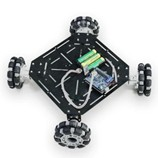
\includegraphics[width=\linewidth]{figures/Chapter 3/rectangular_square_chassis.jpg}
        \caption{Rectangular}
    \end{subfigure}
    \hfill
    \begin{subfigure}[b]{0.3\textwidth}
        \centering
        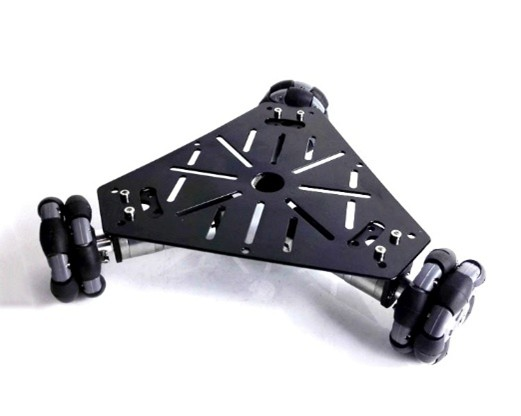
\includegraphics[width=\linewidth]{figures/Chapter 3/triangular_chassis.jpg}
        \caption{Triangular}
    \end{subfigure}
    \hfill
    \begin{subfigure}[b]{0.3\textwidth}
        \centering
        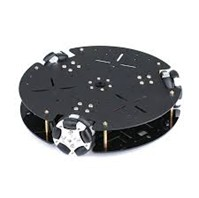
\includegraphics[width=\linewidth]{figures/Chapter 3/circular_chassis.jpg}
        \caption{Circular}
    \end{subfigure}
    \caption{Chassis Configuration Options}
    \label{fig:chassis_options}
\end{figure}

\begin{itemize}
    \item \textbf{Rectangular/Square Chassis:}
    \begin{itemize}
        \item \textbf{Description:} A four-sided frame where wheels are typically mounted at the corners.
        \item \textbf{Mechanical Profile:} This is the most common shape in robotics due to the ease of mounting rectangular PCBs and batteries. However, this profile requires a 4-wheel 90\degree\ omni-drive system like the mecanum wheel configuration. This would increase the costs significantly, especially when we scale the number of robots to 3 or 4 and each wheel requires a motor to drive it.
    \end{itemize}
    \item \textbf{Triangular Chassis:}
    \begin{itemize}
        \item \textbf{Description:} A three-sided frame, where wheels are mounted at the center of each edge or at the vertices.
        \item \textbf{Mechanical Profile:} This is the most "minimalist" design, offering the lowest weight. While it perfectly aligns with the 120\degree\ motor orientation, the tapered edges provide very little surface area for mounting high-level computing boards and sensors, which are typically rectangular. This often leads to "overhang," where sensitive electronics protrude beyond the protection of the chassis.
    \end{itemize}
    \item \textbf{Circular Chassis:}
    \begin{itemize}
        \item \textbf{Description:} A disk-shaped platform where motors are mounted 120\degree\ apart along the perimeter.
        \item \textbf{Mechanical Profile:} The circular design is the most balanced for holonomic robots. It provides a uniform radius from the center of rotation to any point on the perimeter, ensuring that the robot's footprint remains identical regardless of its heading.
    \end{itemize}
\end{itemize}

\paragraph{B. The Selection Matrix}
The configurations were scored based on the specific needs of the Sirius swarm, where multiple robots must operate in close proximity.

\begin{table}[H]
\centering
\caption{Chassis Selection Matrix}
\resizebox{\textwidth}{!}{%
\begin{tabular}{|l|c|c|c|c|c|c|c|}
\hline
\multirow{2}{*}{\textbf{Criteria}} & \multirow{2}{*}{\textbf{Weights}} & \multicolumn{2}{c|}{\textbf{Rectangular}} & \multicolumn{2}{c|}{\textbf{Circular}} & \multicolumn{2}{c|}{\textbf{Triangular}} \\ \cline{3-8} 
 &  & Rating/5 & Score & Rating/5 & Score & Rating/5 & Score \\ \hline
Mounting Surface area & 5 & 5 & 25 & 5 & 25 & 2 & 10 \\ \hline
No of wheels & 4 & 1 & 4 & 5 & 20 & 5 & 20 \\ \hline
Collision Avoidance Ease & 4 & 2 & 8 & 5 & 20 & 3 & 12 \\ \hline
Weight Efficiency & 3 & 3 & 9 & 4 & 12 & 5 & 15 \\ \hline
Structural Integrity & 3 & 5 & 15 & 4 & 12 & 3 & 9 \\ \hline
\textbf{Final Scores} &  &  & \textbf{61} &  & \textbf{89} &  & \textbf{66} \\ \hline
\end{tabular}%
}
\end{table}

\paragraph{C. Detailed Rationale for the Circular Design}
The circular geometry was selected as the optimal chassis configuration for the following engineering reasons:
\begin{enumerate}
    \item \textbf{Constant Sweep Area (Rotational Symmetry):} In swarm robotics, collision avoidance is a primary challenge. A circular chassis has a constant radius ($R$). This means that if the robot rotates in place, its "occupancy" in the 2D map does not change. Unlike a rectangular or triangular robot—which might hit an obstacle only when it turns—the circular Sirius robot can rotate freely without increasing its risk of collision. This simplifies the navigation algorithms significantly.
    \item \textbf{Optimized Internal "Real Estate":} The graduation project requires a significant hardware stack: a microcontroller, motor drivers, a high-level computing board, a battery, a 2D lidar, and the depth camera. A circular plate with a 30 cm diameter provides a much larger surface area than a triangular plate of the same width. This allows for a "cleaner" layout, better cable management, and the ability to mount components centrally to keep the Center of Gravity (CoG) perfectly aligned with the center of rotation.
    \item \textbf{Mechanical Stability \& Load Distribution:} The 120\degree\ motor placement on a circular disk ensures that the load is distributed evenly across all three points of contact. In a triangular design, the "sharp" corners are structural weak points; in a circular design, the stress from the motor mounts is distributed more uniformly along the arc of the plate, reducing the risk of material fatigue or warping over time.
    \item \textbf{Aesthetic and Functional Uniformity:} As a swarm of three autonomous robots, uniformity is key. The circular design allows for a modular "stack" where each layer (Base, Control, Perception) can be identical across all three units, facilitating interchangeable parts and easier mass assembly.
\end{enumerate}

\newpage
\subsubsection{Material Selection of Robot Plate}
In this section we will discuss the Robot Plate material selection.

\paragraph{A. Available Materials}
After a lot of surveying and discussion in choosing the best materials in the market and through our research that could be used for our Robot that satisfies our targets. We will discuss the available options, their associated advantages and disadvantages, and how they interact to providing the desired performance.

\begin{table}[H]
    \centering
    \caption{Available Materials}
    \begin{tabular}{|l|c|c|c|l|}
    \hline
    \textbf{Material} & \textbf{Yield Stress (MPa)} & \textbf{Density (Kg/m$^3$)} & \textbf{Young’s Modulus (Gpa)} & \textbf{Price} \\
    \hline
    Aluminum & 100-500 & 2700 & 69 & Mod. High \\
    \hline
    Acrylic & 60-80 & 1200 & 3.2 & Moderate \\
    \hline
    Steel & 250-700 & 7900 & 200 & Moderate \\
    \hline
    \end{tabular}
\end{table}

Using Steel for the plates in the robot is a strong and durable choice. It’s tough and doesn’t easily get deflected plus it’s not too expensive. The disadvantage of it is that it’s too heavy to be used in our Robots.

Aluminum is a good choice for our Robots but, it has downside of having a high cost between the other two options, as it good in part of being relatively low in weight and rigid enough.

Last for Acrylic is the lowest in strength, can crack under impact or stress concentrations, but have the lowest weight and used as insulator that won’t cause shorts and lowest in the price.

\paragraph{B. Plate Material selection Matrix}
For swarm robots weight is critical for battery life and mobility. Our target here is to select the most suitable material to meet our defined targets.

\begin{table}[H]
\centering
\caption{Plate Material Selection Matrix}
\resizebox{\textwidth}{!}{%
\begin{tabular}{|l|c|c|c|c|c|c|c|}
\hline
\multirow{2}{*}{\textbf{Criteria}} & \multirow{2}{*}{\textbf{Weights}} & \multicolumn{2}{c|}{\textbf{Steel}} & \multicolumn{2}{c|}{\textbf{Aluminum}} & \multicolumn{2}{c|}{\textbf{Acrylic}} \\ \cline{3-8} 
 &  & Rating/5 & Score & Rating/5 & Score & Rating/5 & Score \\ \hline
Stiffness to Weight Ratio & 4 & 5 & 20 & 4 & 16 & 2 & 8 \\ \hline
Manufacturability & 5 & 4 & 20 & 5 & 25 & 5 & 25 \\ \hline
Price & 4 & 5 & 20 & 3 & 12 & 5 & 20 \\ \hline
Density & 5 & 1 & 5 & 4 & 20 & 5 & 25 \\ \hline
\textbf{Final Scores} &  &  & \textbf{65} &  & \textbf{73} &  & \textbf{78} \\ \hline
\end{tabular}%
}
\end{table}

Based on the selection matrix table resulted in that Acrylic is the best option for its weight over steel and aluminum in density and Manufacturability although it has the least score in stiffness to weight Ratio, but we will approve it’s durability in stress analysis.

\newpage

\subsubsection{Evaluation of Materials}
The main structural component of the robot is a cylindrical “wall” of housing that serves as the backbone for all internal components, sensors, and the three-omni-wheel drivetrain. The material must resist warping while staying within the 5kg mass constraint.
These materials were evaluated for the construction of cylindrical housing: PLA (3D-printed), Sheet metal (Aluminum).

\begin{figure}[H]
    \centering
    \begin{subfigure}[b]{0.45\textwidth}
        \centering
        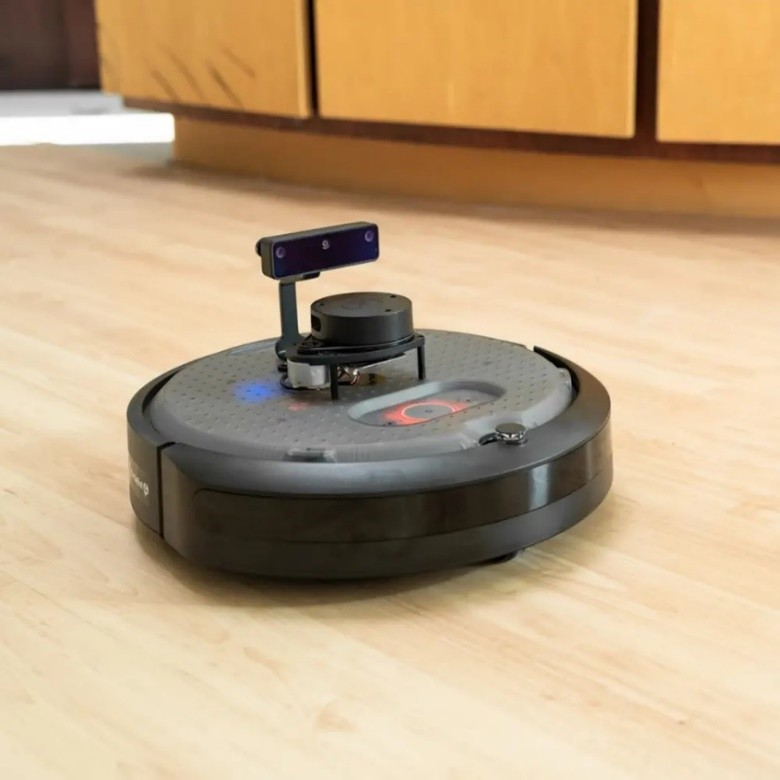
\includegraphics[width=\linewidth]{figures/Chapter 3/Inspiration_design_for_the_chasis_v1.jpg}
        \caption{Design Inspiration V1}
    \end{subfigure}
    \hfill
    \begin{subfigure}[b]{0.45\textwidth}
        \centering
        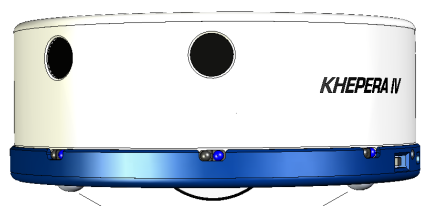
\includegraphics[width=\linewidth]{figures/Chapter 3/Inspiration_design_for_the_chasis_v2.png}
        \caption{Design Inspiration V2}
    \end{subfigure}
    \caption{Inspiration Design for The Chassis}
    \label{fig:chassis_inspiration}
\end{figure}


\paragraph{Candidate Materials Analysis}
\begin{enumerate}
    \item \textbf{3D-Printed Polylactic Acid (PLA):} PLA is the most versatile option for rapid prototyping. It allows for the creation of complex internal fixations and integrated sensor mounts that would be impossible to manufacture with traditional methods.
    \item \textbf{Aluminum Sheet Metal (6061 Alloy):} Aluminum offers the highest strength-to-weight ratio and provides excellent protection for internal electronics.
\end{enumerate}

\paragraph{Material Selection Matrix}

\begin{table}[H]
\centering
\caption{Chassis Construction Selection Matrix}
\begin{tabular}{|l|c|c|c|c|c|}
\hline
\multirow{2}{*}{\textbf{Criteria}} & \multirow{2}{*}{\textbf{Weights}} & \multicolumn{2}{c|}{\textbf{Sheet Metal Aluminum}} & \multicolumn{2}{c|}{\textbf{PLA-3D-Printed}} \\ \cline{3-6} 
 &  & Rating/5 & Score & Rating/5 & Score \\ \hline
Manufacturability & 5 & 3 & 15 & 5 & 25 \\ \hline
Rigidity & 4 & 5 & 20 & 3 & 12 \\ \hline
Internal Fixation Integration & 3 & 3 & 9 & 4 & 12 \\ \hline
Weight & 3 & 4 & 12 & 5 & 15 \\ \hline
\textbf{Final Scores} &  &  & \textbf{56} &  & \textbf{64} \\ \hline
\end{tabular}
\end{table}

Based on the selection matrix above, the 3D-printed PLA was selected as the primary material for the cylindrical wall and internal fixations. The deciding factor was the integration of complex geometry.
Since the robot utilizes a 3-omni-wheel configuration, the motor mounts must be positioned at exactly 120\degree\ intervals.


\subsubsection{Actuator Sizing and Motor Selection}
The selection of actuators is a critical phase in the mechanical design of the Ausrabot robot. The motors must provide sufficient torque to overcome static friction and inertia while maintaining a rotational speed that meets the minimum linear velocity requirement of 0.2 m/s. This section outlines the requirements determined by the robot's kinematics and justifies the final component choice through a weighted selection matrix.

\paragraph{A. Determination of Motor Requirements}
To size the actuators correctly, the desired robot performance must be mapped to the individual wheel requirements. Unlike a standard differential drive, a 3-wheel omni-directional configuration at dictates that wheel speeds are vector components of the robot’s total velocity.
\begin{enumerate}
    \item \textbf{Kinematic Velocity Requirements:} For a robot to achieve a translational velocity of 0.2 m/s, the individual wheel speeds must account for the geometry of the 120 degree configuration of the omni wheels. As detailed in the Kinematics Section, the relationship between the robot velocity and individual wheel velocity is defined by the transformation matrix. To ensure the robot can reach 0.2 m/s in any direction and maintain rotational stability:
    \begin{itemize}
        \item \textbf{Calculated Minimum Motor RPM:} Considering the wheel radius (r = 0.0325m) and the kinematic constraints, the motors must provide a rated speed of at least 85–90 RPM.
        \item \textbf{Target Linear Velocity (v):} > 0.2 m/s.
    \end{itemize}
    \item \textbf{Torque Requirements:} The motor must overcome the Force of Inertia ($F_i$) and the Rolling Resistance ($F_{rr}$). Given the Nylon rollers of the Omni-wheels on indoor flooring, a rolling resistance coefficient ($C_{rr}$) of 0.02 is assumed for a maximum robot mass of 5 kg.
    \begin{itemize}
        \item \textbf{Total Force ($F_{total}$):} Approximately 1.98 N (calculated from $m a + m g C_{rr}$).
        \item \textbf{Required Rated Torque:} To handle the 5 kg payload and provide a safety margin for slopes or surface irregularities, the motors must provide a rated torque of at least 0.8–1.0 kg·cm.
    \end{itemize}
\end{enumerate}

\paragraph{B. Comparative Analysis of Available Actuators}
Three motors were evaluated based on the 12V power constraint and the physical requirements of the swarm units.

\begin{enumerate}
    \item \textbf{JGA25-370 (High Speed, 130 RPM):} A standard spur-geared DC motor. While it offers high speed and a compact form factor, it possesses lower torque compared to worm-gear alternatives, which may struggle with the maximum 5 kg payload.
    \item \textbf{JGY-370-1285 (Worm Gear, 98 RPM):} This motor features a worm-gear reduction which provides significantly higher torque and a self-locking mechanism. The 98 RPM output perfectly matches the required range determined by the kinematic analysis while ensuring high pushing force.
    \item \textbf{E-S Planetary Geared Motor (182 RPM):} A high-performance planetary motor. While technically superior in speed, its physical length > 90mm with encoder) combined with the omni wheel, coupler, shaft, bearing and brackets would cause the robot's total radius to exceed the 0.3m (30 cm) limit established in the design requirements.
\end{enumerate}

\begin{figure}[H]
    \centering
    \begin{subfigure}[b]{0.32\textwidth}
        \centering
        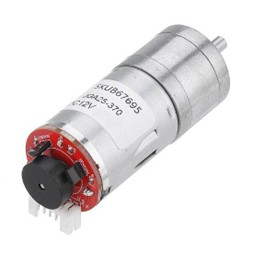
\includegraphics[width=\linewidth]{figures/Chapter 3/JGA25-370_motor.jpg}
        \caption{JGA25-370}
        \label{fig:jga25}
    \end{subfigure}
    \hfill
    \begin{subfigure}[b]{0.32\textwidth}
        \centering
        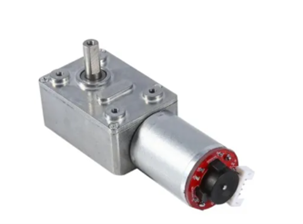
\includegraphics[width=\linewidth]{figures/Chapter 3/JGY-370-1285_motor.png}
        \caption{JGY-370 (Worm)}
        \label{fig:jgy370}
    \end{subfigure}
    \hfill
    \begin{subfigure}[b]{0.32\textwidth}
        \centering
        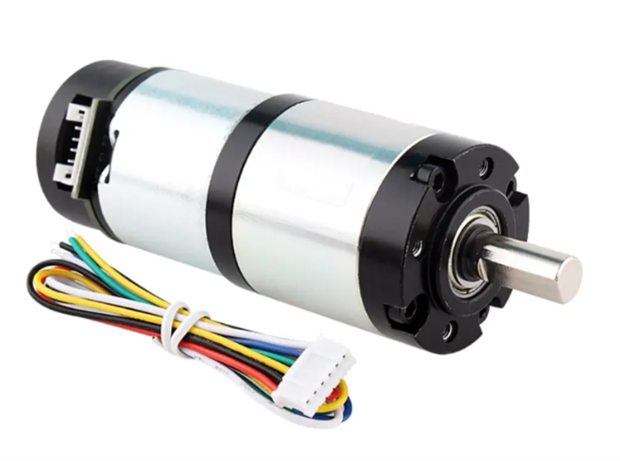
\includegraphics[width=\linewidth]{figures/Chapter 3/E-S_Planetary_Geared_Motor.png}
        \caption{E-S Planetary}
        \label{fig:es_planetary}
    \end{subfigure}
    \caption{Comparative view of evaluated motors}
    \label{fig:motor_comparison}
\end{figure}

\paragraph{C. Actuator Selection Criteria}
To objectively determine the best actuator for the swarm, five key criteria were established:
\begin{enumerate}
    \item \textbf{Torque Performance (Weight 5):} The ability of the motor to drive a 5 kg robot consistently without overheating or stalling, especially during high-torque swarm maneuvers.
    \item \textbf{Size/Footprint (Weight 5):} The physical length and mounting orientation must allow the three motors to be placed 120 apart without exceeding the 30 cm robot diameter limit.
    \item \textbf{Speed/RPM (Weight 4):} The motor must meet or exceed the 85-90 RPM threshold to maintain the 0.2 m/s target velocity across all translation vectors.
    \item \textbf{Self-Locking/Stability (Weight 3):} The inherent ability of the gear system to hold its position when unpowered. This is vital for static mapping and station-keeping in a swarm.
    \item \textbf{Unit Cost (Weight 2):} Since the project involves a swarm of three robots (requiring 9 motors in total), the individual price per unit is a significant factor in the overall project budget.
\end{enumerate}

\paragraph{D. Selection Matrix}
The following matrix evaluates the motors against the project constraints. For "Torque Performance," the highest weight is assigned as it is critical for handling the 5 kg design limit.

\begin{table}[H]
\centering
\caption{Motor Selection Matrix}
\resizebox{\textwidth}{!}{%
\begin{tabular}{|l|c|c|c|c|c|c|c|}
\hline
\multirow{2}{*}{\textbf{Criteria}} & \multirow{2}{*}{\textbf{Weights}} & \multicolumn{2}{c|}{\textbf{JGA25-370}} & \multicolumn{2}{c|}{\textbf{JGY-370 (Worm)}} & \multicolumn{2}{c|}{\textbf{E-S Planetary}} \\ \cline{3-8} 
 &  & Rating/5 & Score & Rating/5 & Score & Rating/5 & Score \\ \hline
Torque Performance & 5 & 2 & 10 & 4 & 20 & 5 & 25 \\ \hline
Size/Footprint & 4 & 4 & 16 & 3 & 12 & 1 & 4 \\ \hline
Speed/RPM & 4 & 4 & 16 & 3 & 12 & 5 & 20 \\ \hline
Self-Locking /Stability & 3 & 2 & 6 & 4 & 12 & 3 & 9 \\ \hline
Unit cost & 3 & 5 & 15 & 5 & 15 & 2 & 6 \\ \hline
\textbf{Final Scores} &  &  & \textbf{63} &  & \textbf{71} &  & \textbf{64} \\ \hline
\end{tabular}%
}
\end{table}

\paragraph{E. Selection Rationale}
The JGY-370 Worm Gear motor (98 RPM) was selected as the optimal actuator for the Ausra robot.
The primary driver for this selection was the high rated torque provided by the worm-gear reduction. As the robot is designed for a maximum mass of 5 kg, the JGA25-370 was deemed insufficient for reliable long-term operation under full load. The JGY-370's 98 RPM speed is well-optimized for the 3-wheel kinematics, providing enough headroom to achieve the 0.2 m/s target velocity without excessive power consumption.
A unique advantage of the JGY-370 is its self-locking property. In a swarm environment, the ability of the robot to maintain its position without consuming power (braking) is highly beneficial for static 2D mapping tasks and formation holding. Although the worm-gear orientation requires careful mounting, it fits within the 30 cm radius constraint, unlike the E-S Planetary motor which was rejected for its prohibitive length and high unit cost.


\newpage

\section{Detailed CAD Design}
\label{sec:cad_design}

\subsection{CAD Modeling \& Geometry}
The physical realization of the Ausra robot follows modular "Tri-Level Stack" architecture. This design allows for a clear separation between high-current power systems, low-level control logic, and high-level perception hardware. The assembly was modeled in SolidWorks to ensure precise tolerances, specifically for the radial symmetry of the locomotion system. The assembly of the full robot is based on mounting all the hardware components we selected previously.

\begin{figure}[H]
    \centering
    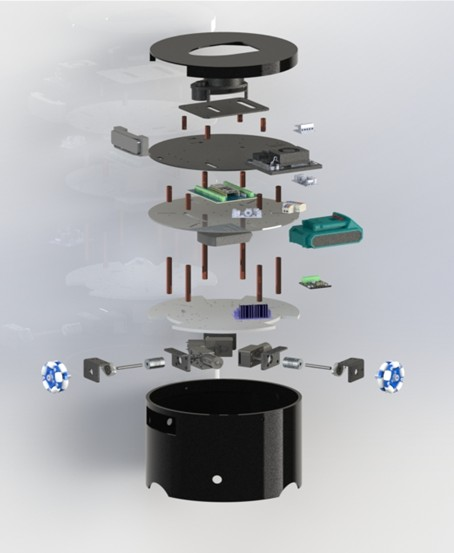
\includegraphics[width=0.8\linewidth]{figures/Chapter 3/vertical_exploded_view.jpg}
    \caption{Vertical Exploded View of the Robot Stack}
    \label{fig:exploded_stack}
\end{figure}

\newpage

\subsubsection{Layer 1: The Locomotion \& Power Drive Base Plate}
The first layer of the Ausra robot acts as the structural and mechanical foundation of the entire system. Its primary role is to serve as a rigid, high-torque platform that translates digital control vectors into physical movement. In an omni-directional swarm robot, the base plate must not only support the static weight of the upper electronics stack but also withstand the dynamic, multi-directional forces generated during rapid translations and rotations. Consequently, the design of this layer focuses heavily on structural rigidity, mechanical load distribution, and power transmission integrity.

\begin{figure}[H]
    \centering
    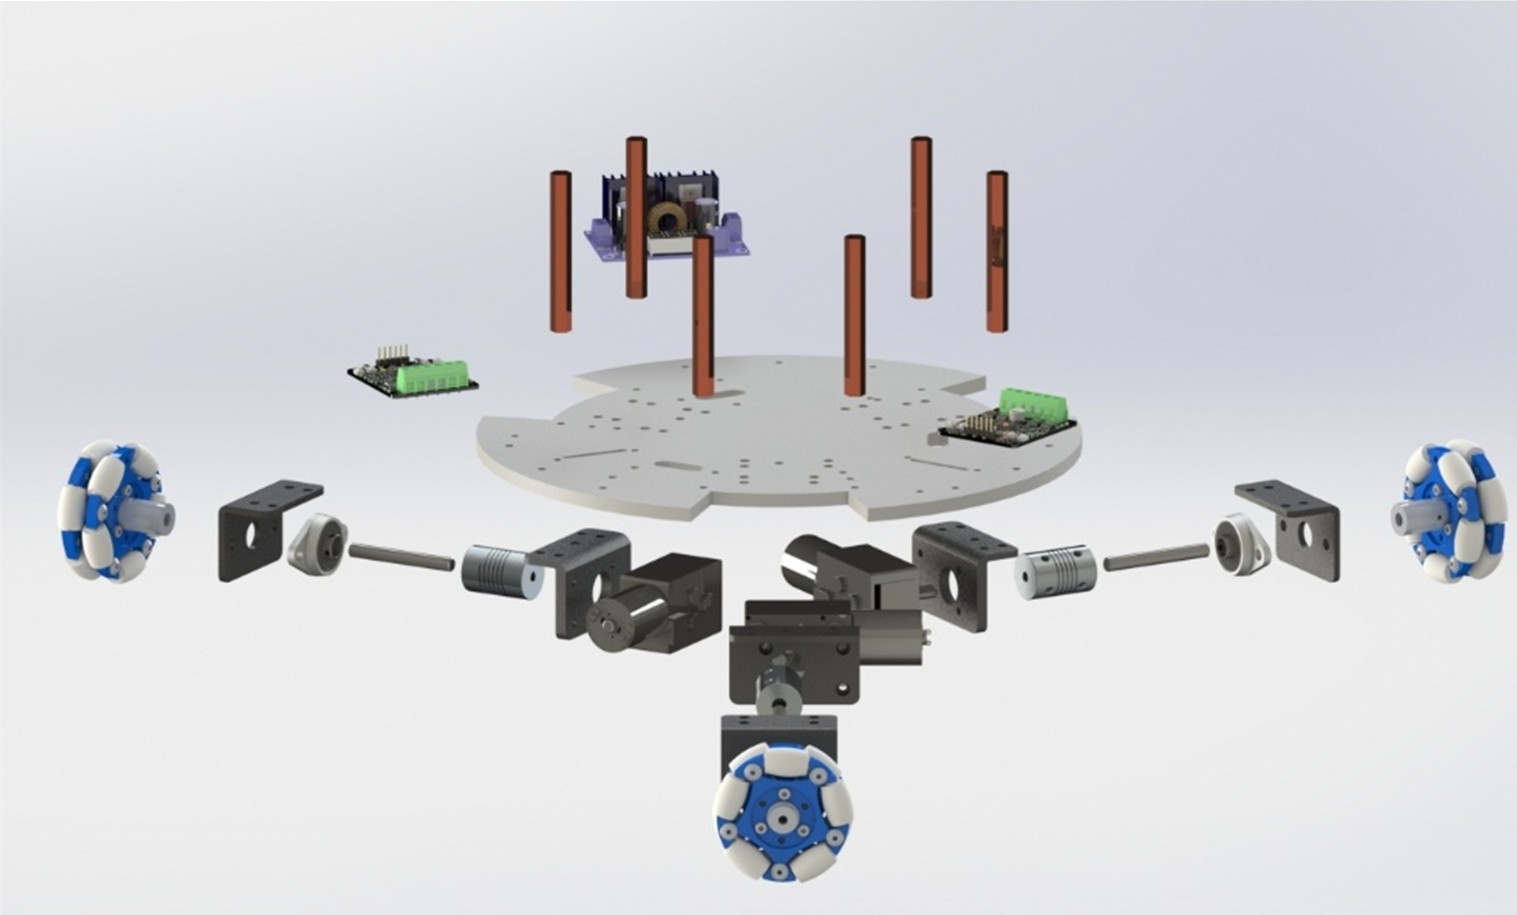
\includegraphics[width=\linewidth]{figures/Chapter 3/Locomotion_and_Power_Drive_Base_Plate_exploded_view.jpg}
    \caption{Base Plate Exploded View}
    \label{fig:base_plate}
\end{figure}

\newpage
\paragraph{A. The Actuation Assembly and Radial Support System}
A common failure point in mobile robotics is the excessive radial load applied directly to motor shafts, especially during the lateral "sliding" maneuvers typical of omni-directional movement. To ensure the longevity of the JGY-370 worm-gear motors, a sophisticated dual-point support system was engineered. Each motor is anchored to the base plate using high-strength motor brackets positioned at precise radial intervals. This symmetry is critical for maintaining balanced kinematics and a centralized center of mass.
However, the standout feature of this layer is the auxiliary bearing support system. Unlike hobby-grade designs where wheels are cantilevered directly off the motor gearbox, the Ausra robot utilizes an additional bearing bracket for each drive line. This bracket houses a precision ball bearing that supports the end of the driveshaft just before it interfaces with the wheel. By introducing this second point of contact, any bending moments or perpendicular shocks encountered by the wheels are absorbed by the bearing and the chassis plate itself, rather than the motor’s internal brass gears. This mechanical isolation significantly reduces the risk of shaft deformation and gear stripping, ensuring the robot remains operational under its maximum 5kg payload.

\begin{figure}[H]
    \centering
    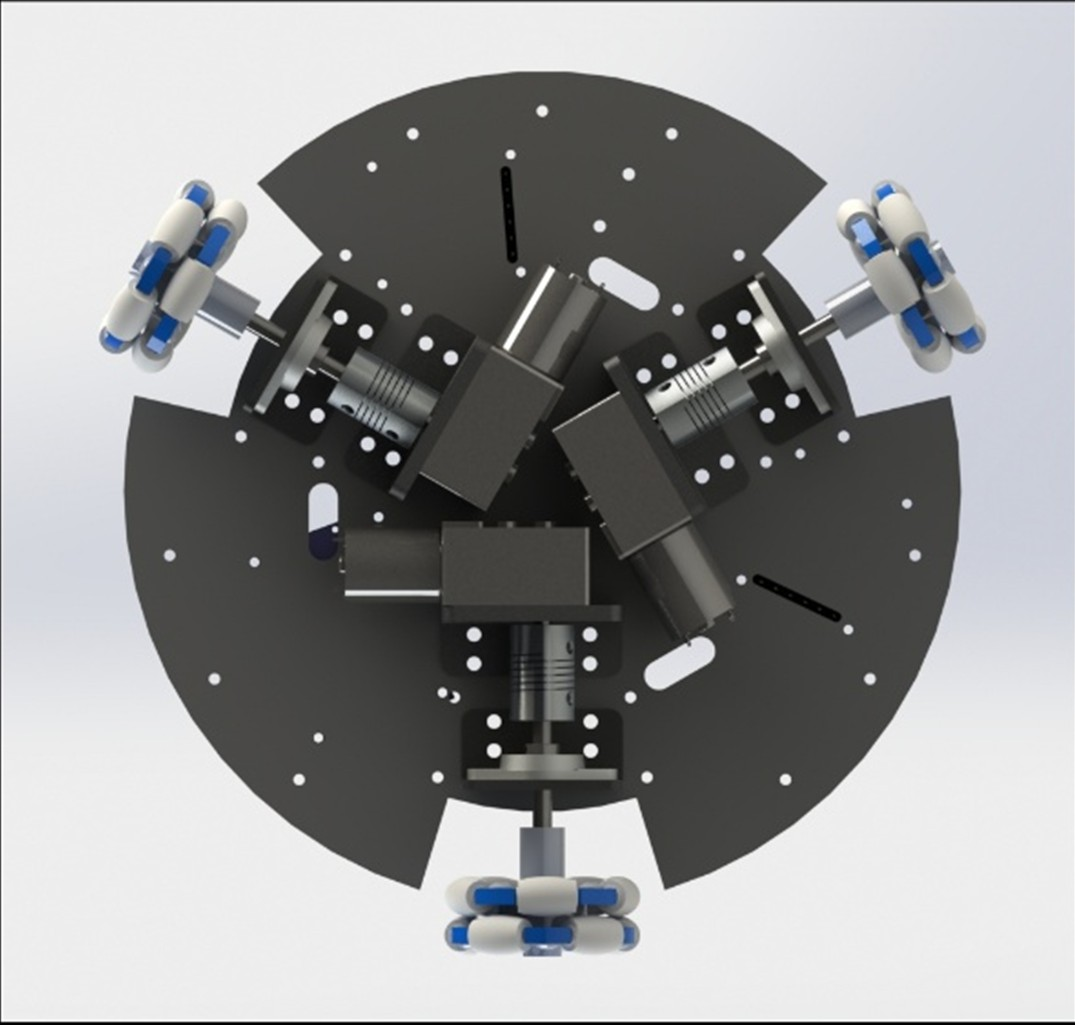
\includegraphics[width=0.9\linewidth]{figures/Chapter 3/Actuation_Assembly_and_Radial_Support_System.jpg}
    \caption{Actuation Assembly and Radial Support}
    \label{fig:radial_support}
\end{figure}

\paragraph{B. Precision Power Transmission and Coupling}
To bridge the gap between the centrally mounted motors and the peripheral Omni-wheels, a robust power transmission line was implemented. Each drive line utilizes a precision-ground steel driveshaft with a length of 50 mm and a diameter of 8mm. Steel was selected specifically for its high torsional rigidity; it ensures that the shaft can transmit the high stall torque of the worm-gear reduction without twisting or flexing, which would otherwise introduce inaccuracies in the robot's odometry and SLAM data.
The transmission is managed through a dual-coupling strategy designed for zero-slip performance. A primary coupler interfaces the 6 mm D-shaped output of the motor to the 8 mm steel shaft. At the distal end, an Aluminum wheel coupler secures the shaft to the Omni-wheel. Aluminum was chosen for the wheel interface because it provides a lightweight yet durable "bite" on the shaft. These couplers are secured using industrial-grade set-screws, ensuring that every rotation of the motor is perfectly mirrored by the wheel—a fundamental requirement for the high-precision coordination needed in swarm formations.

\begin{figure}[H]
    \centering
    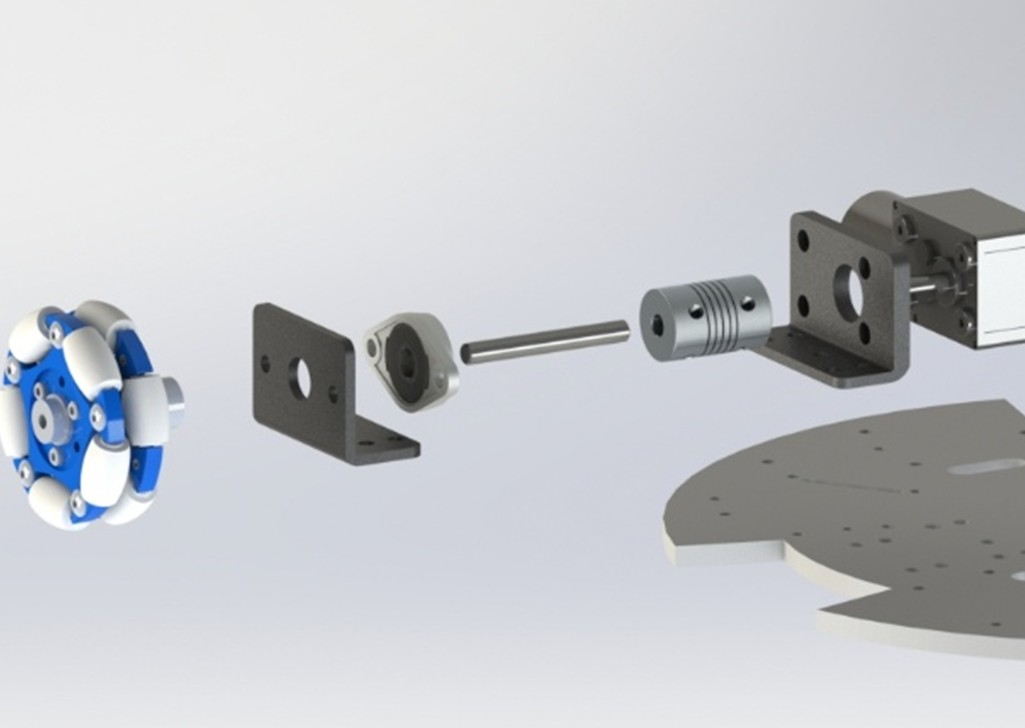
\includegraphics[width=0.6\linewidth]{figures/Chapter 3/Precision_Power_Transmission_and_Coupling.jpg}
    \caption{Precision Power Transmission and Coupling}
    \label{fig:power_trans}
\end{figure}

\paragraph{C. Integrated Power Control and Signal Integrity}
The top surface of the first layer functions as the high-current "Engine Room" of the robot. To protect the sensitive perception sensors and microcontrollers on the upper layers from Electromagnetic Interference (EMI) and electrical noise, the high-power components are localized here. Two Cytron motor drivers are mounted directly to the base plate, positioned in close proximity to the actuators. This strategic placement minimizes the length of high-current wiring, which in turn reduces voltage drops and parasitic inductance that can occur during rapid motor reversals.
Furthermore, this layer includes a dedicated Buck Converter specifically for logic regulation. This converter steps down the main 12V battery supply to a stable logic-level voltage for the motor drivers. By isolating the driver logic with a dedicated regulator on the base layer, the system gains a layer of protection against "brownouts." Even during peak current draws—such as when the robot must overcome high static friction—the drivers' logic remains stable, ensuring the ESP32 always maintains consistent control over the actuators.

\begin{figure}[H]
    \centering
    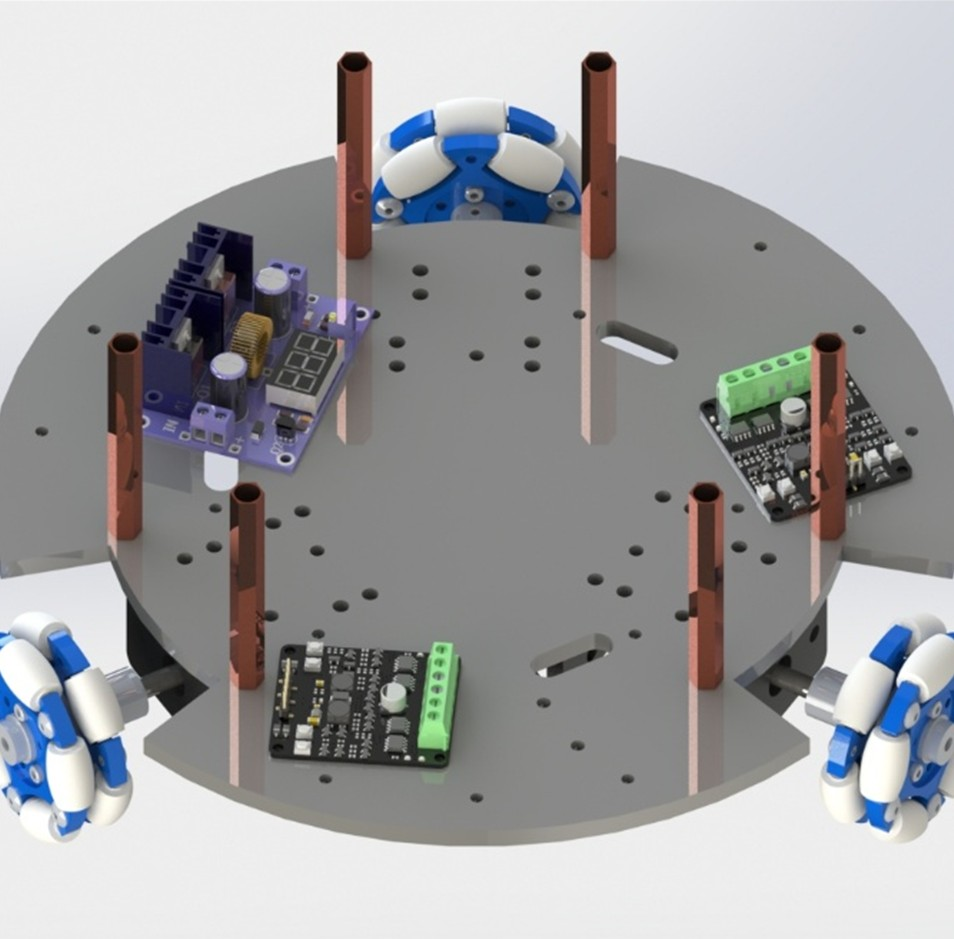
\includegraphics[width=0.6\linewidth]{figures/Chapter 3/Integrated_Power_Control_and_Signal_Integrity.jpg}
    \caption{Integrated Power Control and Signal Integrity}
    \label{fig:power_control}
\end{figure}

\subsubsection{Layer 2: Energy Storage \& Signal Processing}
The middle layer of the Sirius robot serves as the "Nervous System" of the platform, acting as the primary junction between the high-current actuation base and the high-level perception stack. Physically, this layer is designed to manage the robot's mass distribution and signal routing. By isolating the microcontroller and power distribution hardware on a dedicated central plate, the design achieves a "buffer zone" that protects sensitive logic signals from the mechanical vibrations of the base and the electromagnetic noise generated by the motors.

\begin{figure}[H]
    \centering
    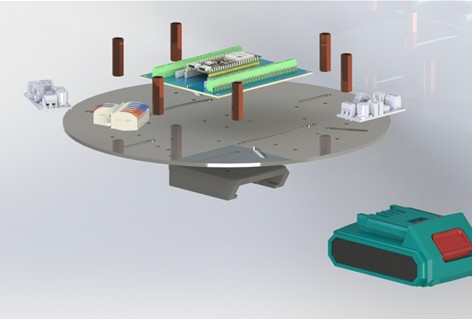
\includegraphics[width=0.6\linewidth]{figures/Chapter 3/Layer_2-_Energy_Storage_and_Signal_Processing.jpg}
    \caption{Layer 2: Energy Storage and Signal Processing}
    \label{fig:layer2_iso}
\end{figure}

\paragraph{A. Battery and Center of Gravity (CoG) Optimization}
One of the most critical factors in the stability of a three-wheeled omni-directional robot is the management of its Center of Gravity (CoG). Because the robot is capable of instantaneous acceleration in any direction, a high CoG would lead to significant tipping moments, causing the wheels to lose traction or the odometry to drift. To mitigate this, the primary energy source (Battery) is secured to the bottom surface of Layer 2.
The battery is housed within a custom-fit, 3D-printed holder designed to prevent any lateral shifting during high-G maneuvers. By mounting the heaviest single component of the robot as low as possible within the central stack, the design ensures a low CoG. This placement provides a stabilizing effect, allowing the robot to execute sharp, high-speed translations while maintaining a level profile. This physical stability is not just a mechanical preference; it is a prerequisite for the high-level SLAM algorithms, which require a stable platform to generate consistent 2D point clouds and depth maps.

\begin{figure}[H]
    \centering
    \begin{subfigure}[b]{0.45\textwidth}
        \centering
        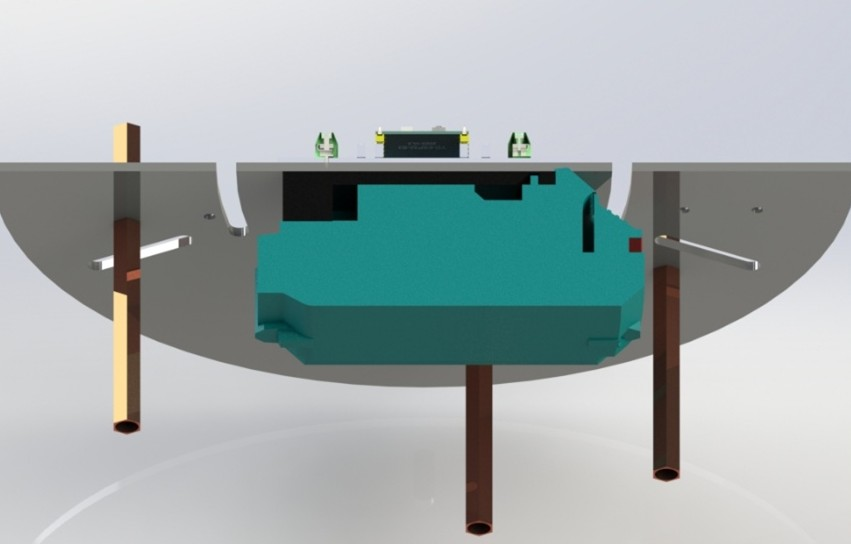
\includegraphics[width=\linewidth]{figures/Chapter 3/Battery_hub_v1.jpg}
        \caption{Battery Hub V1}
    \end{subfigure}
    \hfill
    \begin{subfigure}[b]{0.45\textwidth}
        \centering
        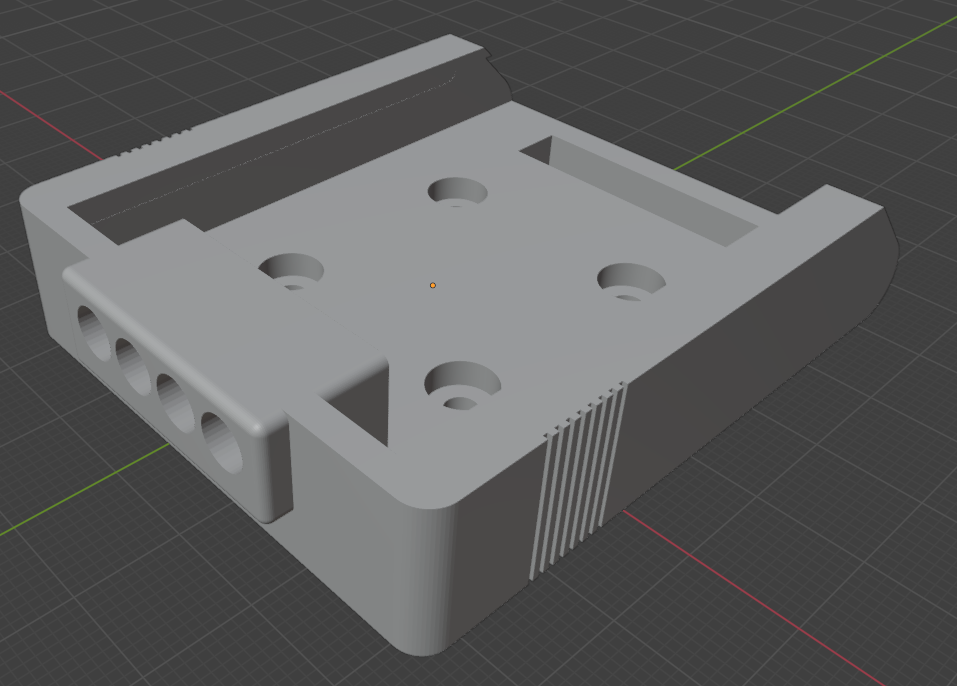
\includegraphics[width=\linewidth]{figures/Chapter 3/battery_hub_3d_printed.png}
        \caption{3D Printed Hub}
    \end{subfigure}
    
    \vspace{1em}
    
    \begin{subfigure}[b]{0.5\textwidth}
        \centering
        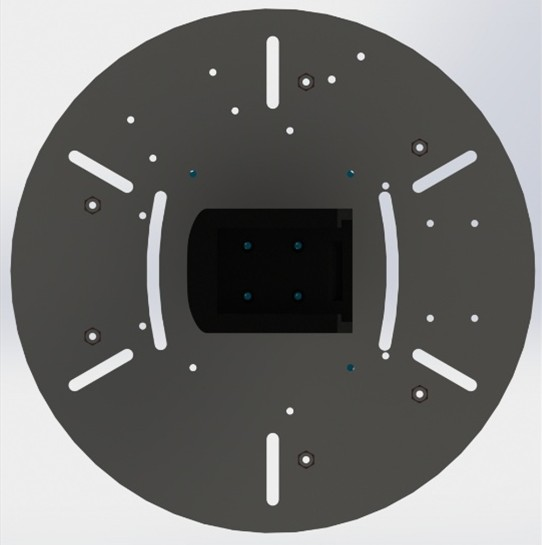
\includegraphics[width=\linewidth]{figures/Chapter 3/COG.jpg}
        \caption{Center of Gravity}
    \end{subfigure}
    
    \caption{Battery Housing and COG Optimization}
    \label{fig:battery_cog}
\end{figure}

\paragraph{B. The Centralized Control Hub and Signal Routing}
The top surface of the second layer is dedicated to the Low-Level Control Group. This hub is centered around the ESP32 microcontroller and its accompanying shield. The shield is a vital component of the "Ausra" architecture, as it allows for secure, vibration-resistant connections for the encoders and motor driver headers. By elevating the microcontroller to the second layer, we provide it with a clear physical separation from the high-current cabling of the base, significantly reducing the risk of "crosstalk" or signal corruption that could lead to erratic motor behavior.
In addition to the microcontroller, this surface hosts several critical power management components:
\begin{itemize}
    \item \textbf{Secondary Buck Converter:} While the first layer uses a regulator for motor logic, this secondary converter is dedicated exclusively to the "clean" 5V and 3.3V rails needed by the ESP32 and auxiliary sensors. This dual-regulator strategy prevents the high-frequency switching noise of the motor drivers from reaching the logic-level processors.
    \item \textbf{Main Power Switch:} Integrated directly into the plate’s perimeter for easy access, the switch provides a physical "hard-cut" for the entire system, ensuring safety during testing and maintenance.
    \item \textbf{SPL Connector Block:} The "Sirius" robot utilizes a "Star Topology" for power distribution rather than daisy-chaining components. The SPL connector acts as a centralized manifold, taking the raw battery voltage and neatly dividing it between the functional layers. This ensures that a failure or short circuit in one subsystem is less likely to affect the others, while also facilitating much cleaner cable management throughout the internal stack.
\end{itemize}
By consolidating these components on Layer 2, the design achieves a modular "Plug-and-Play" architecture. This arrangement allows a researcher to troubleshoot the control logic or swap the battery without needing to dismantle the perception sensors on the top layer or the motor mounts on the base, directly fulfilling the project’s requirement for high serviceability.

\begin{figure}[H]
    \centering
    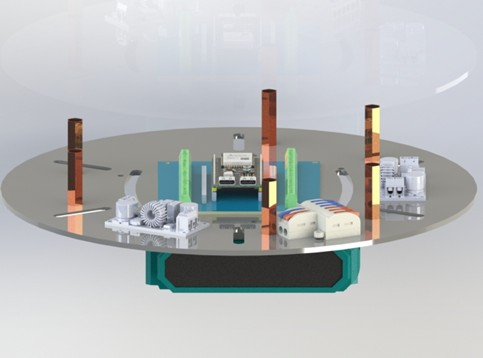
\includegraphics[width=0.7\linewidth]{figures/Chapter 3/Layer_2_assembeled.jpg}
    \caption{Assembled Layer 2 Control Hub}
    \label{fig:layer2_assembled}
\end{figure}

\subsubsection{Layer 3: Perception \& High-Level Intelligence}
The third and final layer of the Ausra robot represents the "apex" of its design, both physically and functionally. While the lower layers handle the brute force of locomotion and the steady logic of power management, the third layer is dedicated entirely to perception, spatial reasoning, and high-level autonomous decision-making. Positioned at the highest point of the stack, this layer provides the sensors with an unobstructed view of the environment, which is paramount for a swarm system tasked with collaborative 2D and 3D mapping.

\paragraph{A. High-Level Computing and Spatial AI Integration}
At the heart of this layer sits the NVIDIA Jetson Orin Nano, which serves as the robot’s primary processing unit. By mounting the Jetson centrally on the top plate, the design ensures that its heat sink remains exposed to ambient air for better thermal management while keeping its mass balanced over the robot's center of rotation. This board runs the heavy ROS2 (Robot Operating System 2) stack, orchestrating the complex communication between individual swarm members and processing the high-bandwidth data coming from the perception sensors.
Adjacent to the computing board is the OAK-D camera, the robot's primary source of "Spatial AI." In this project, the camera isn't just a passive video feed; it is used to perform real-time object detection and depth estimation. To ensure the reliability of this data, the camera is secured via a custom-designed, 3D-printed vibration-dampening holder. This holder is critical because even minor vibrations from the omni-wheels could introduce "jitter" into the depth frames, leading to errors in the SLAM (Simultaneous Localization and Mapping) process. The camera is strategically positioned at the very edge of the plate, angled to maximize its field of view without the robot's own chassis obscuring the "vision" of the lower-plane obstacles.

\paragraph{B. Navigation Sensors and SLAM Hardware}
To achieve precise 2D mapping, the Ausra robot relies on the fusion of LiDAR and inertial data. The mounting strategy for these components on the third layer is driven by the need for geometric accuracy:
\begin{itemize}
    \item \textbf{Elevated LiDAR Platform:} The LiDAR unit is the "eyes" of the 2D SLAM system. To prevent the laser from hitting the robot’s internal components or the protective outer shell, it is mounted on an elevated, secondary plate. This elevation ensures a completely unobstructed 360\degree\ horizontal scan, allowing the robot to detect walls, furniture, and other swarm members at a distance without "blind spots" created by its own structure.
    \item \textbf{Precision IMU Placement:} Orientation data is handled by the Inertial Measurement Unit (IMU), which is fixed to a small, dedicated PCB. For a mechatronics platform, the placement of the IMU is vital; it is mounted as close as possible to the robot's vertical axis of rotation. This minimizes "centripetal acceleration" noise the false readings that occur when an IMU is mounted far from the center ensuring that when the robot spins in place, the orientation data remains clean and drift-free.
\end{itemize}

\begin{figure}[H]
    \centering
    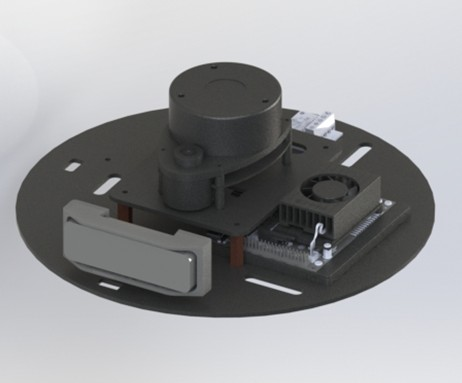
\includegraphics[width=\linewidth]{figures/Chapter 3/layer_3_assembeled.jpg}
    \caption{Assembled Layer 3 Perception Stack}
    \label{fig:layer3_assembled}
\end{figure}


\newpage
\subsubsection{Protective Enclosure (The Outer Shell \& Top Cover)}
Surrounding these three layers is an external wall and cover made from 3D-printed PLA. From a design standpoint, this shell serves two purposes: protecting the sensitive internal electronics from external impacts and providing a clean, aesthetic finish to the swarm unit. Recognizing the need for frequent hardware adjustments during the research phase, the shell was designed as a "split-shell" system. It consists of 2 parts that lock together. This allows us to remove half of the shell to access the Jetson’s ports or the ESP32’s micro-USB connection on the layer below without having to fully disassemble the robot or disturb the calibration of the LiDAR and camera on the top plate.
This layering strategy ensures that the Ausra robot is not just a collection of parts, but a highly organized, modular system where each component is placed specifically to optimize its functional performance and ease of maintenance.

\begin{figure}[H]
    \centering
    \begin{subfigure}[b]{0.45\textwidth}
        \centering
        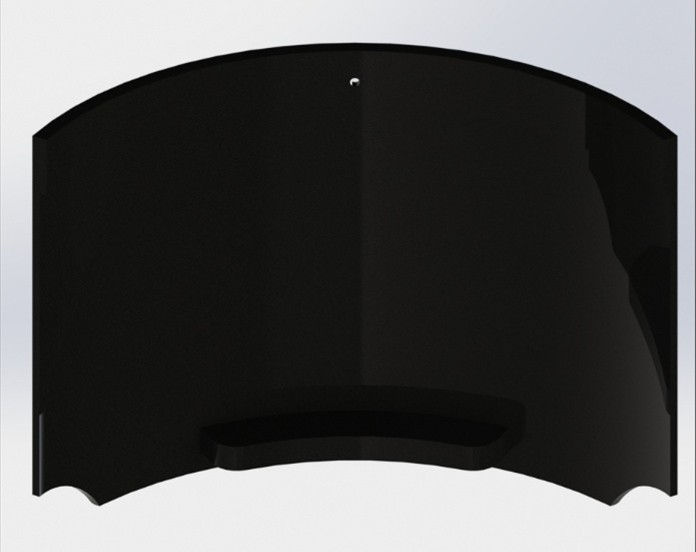
\includegraphics[width=\linewidth]{figures/Chapter 3/3d_printed_enclosure_v1.jpg}
        \caption{Part 1}
    \end{subfigure}
    \hfill
    \begin{subfigure}[b]{0.45\textwidth}
        \centering
        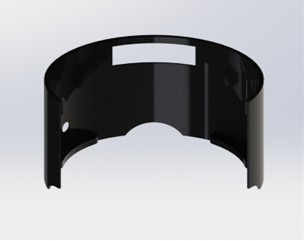
\includegraphics[width=\linewidth]{figures/Chapter 3/3d_printed_enclosure_v2.jpg}
        \caption{Part 2}
    \end{subfigure}
    
    \vspace{0.5cm}
    
    \begin{subfigure}[b]{0.5\textwidth}
        \centering
        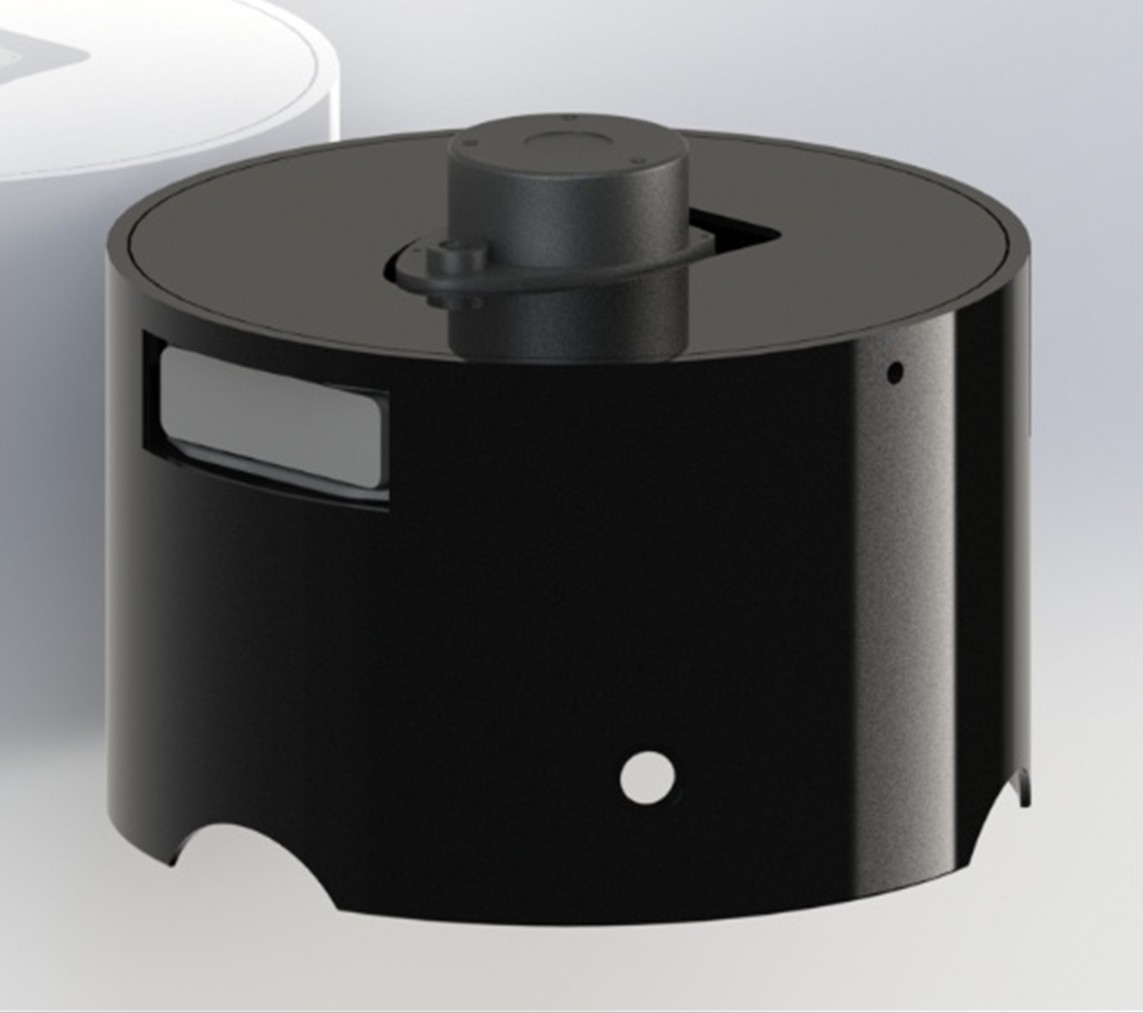
\includegraphics[width=\linewidth]{figures/Chapter 3/3d_printed_enclosure_v3.jpg}
        \caption{Assembled}
    \end{subfigure}
    \caption{Protective Enclosure Design}
    \label{fig:enclosure}
\end{figure}


\newpage
\subsection{Empirical Stress Analysis}
Currently, after selecting the material for the plates of the robot it found that there is two available thicknesses of the same material which are (3mm, 6mm).
We needed to examine all the differences between them by doing stress analysis on each one of them and compare the results. By using the engineering sense, it says that the (6mm) thickness will be better to be used but we needed to make sure if it worthy enough according to the cost and the extra weight.
\begin{itemize}
    \item \textbf{Material:} Acrylic (medium-high impact)
    \item \textbf{Dimensions:} $\phi$260
    \item \textbf{Load:} 50 N
\end{itemize}

\subsubsection{Acrylic Plate of thickness (3mm)}
\begin{figure}[H]
    \centering
    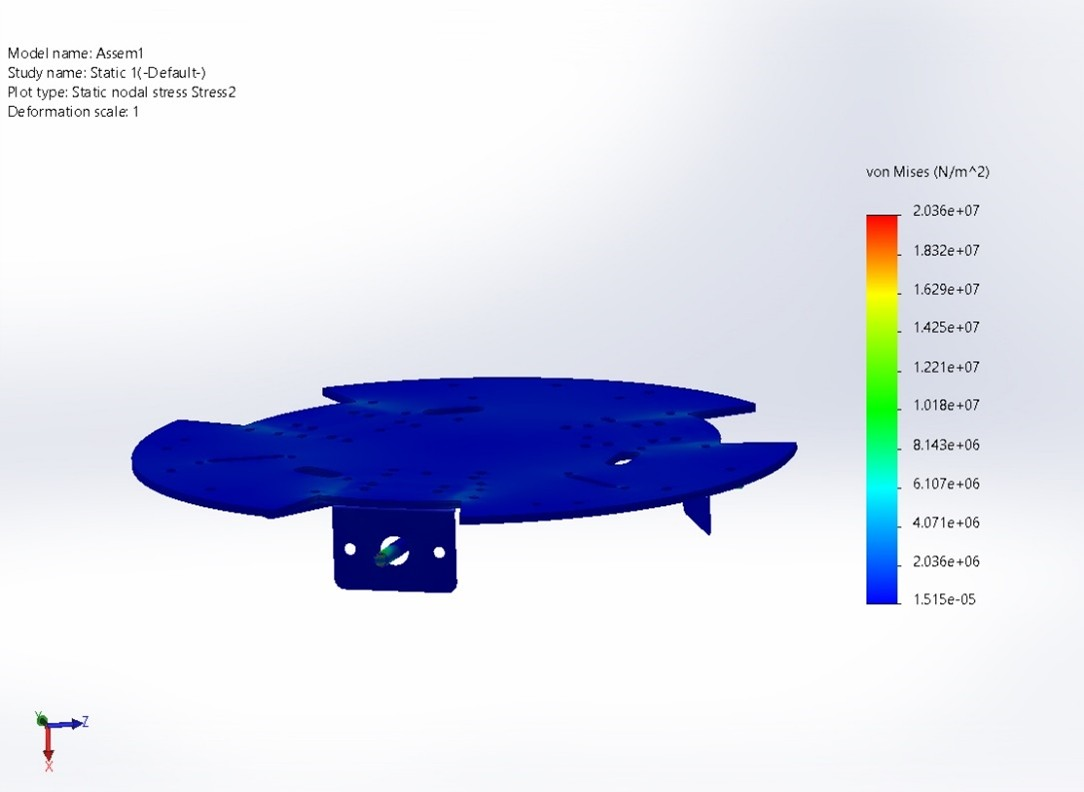
\includegraphics[width=\linewidth]{figures/Chapter 3/Von_mises_Stress3mm.jpg}
    \caption{Von Mises Stress (3mm)}
\end{figure}
\begin{figure}[H]
    \centering
    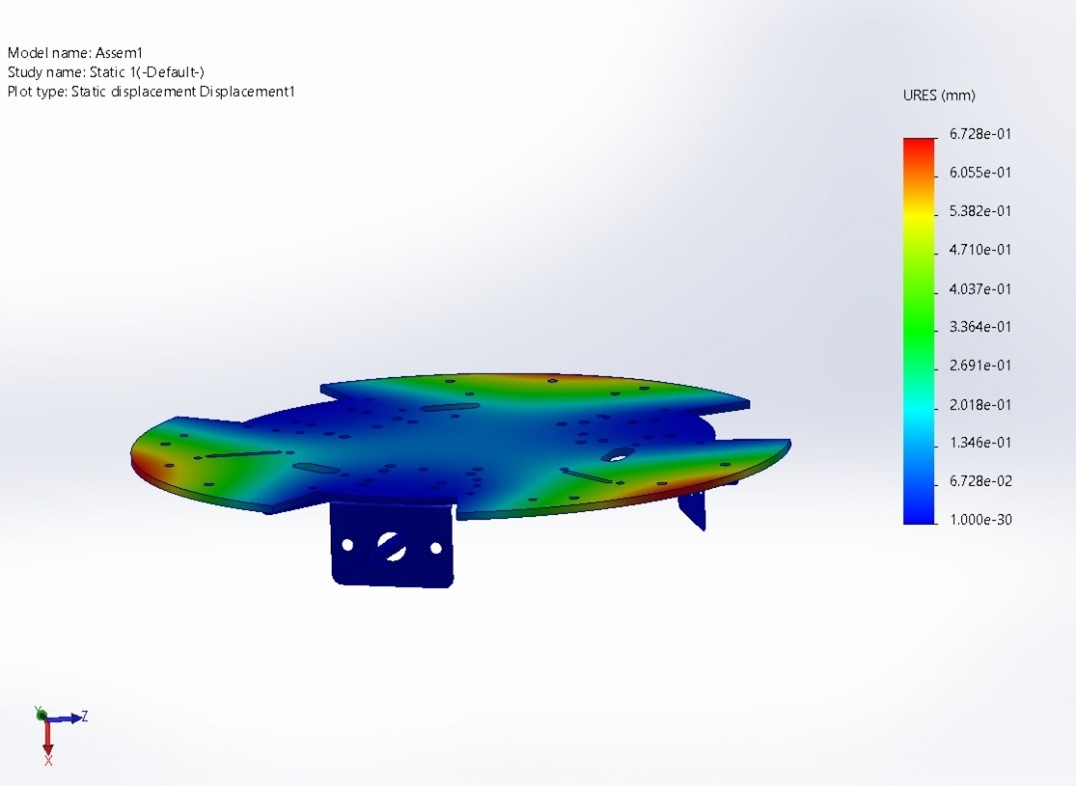
\includegraphics[width=0.85\linewidth]{figures/Chapter 3/Displacement3mm.jpg}
    \caption{Displacement (3mm)}
\end{figure}
\begin{figure}[H]
    \centering
    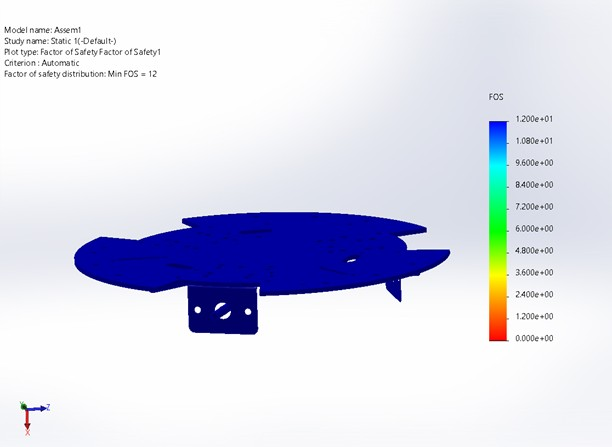
\includegraphics[width=0.85\linewidth]{figures/Chapter 3/Safety_factor3mm.jpg}
    \caption{Safety Factor (3mm)}
\end{figure}

\subsubsection{Acrylic Plate of (6mm)}
\begin{figure}[H]
    \centering
    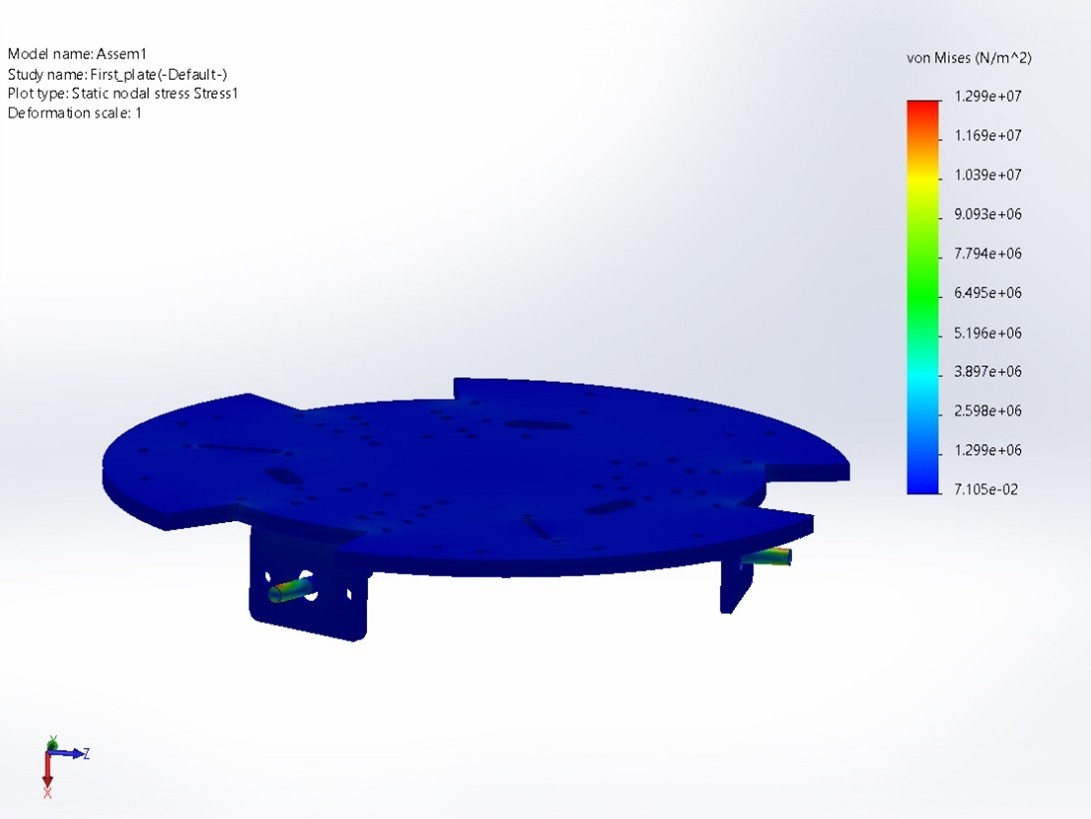
\includegraphics[width=0.75\linewidth]{figures/Chapter 3/Von_mises_Stress6mm.jpg}
    \caption{Von Mises Stress (6mm)}
\end{figure}
\begin{figure}[H]
    \centering
    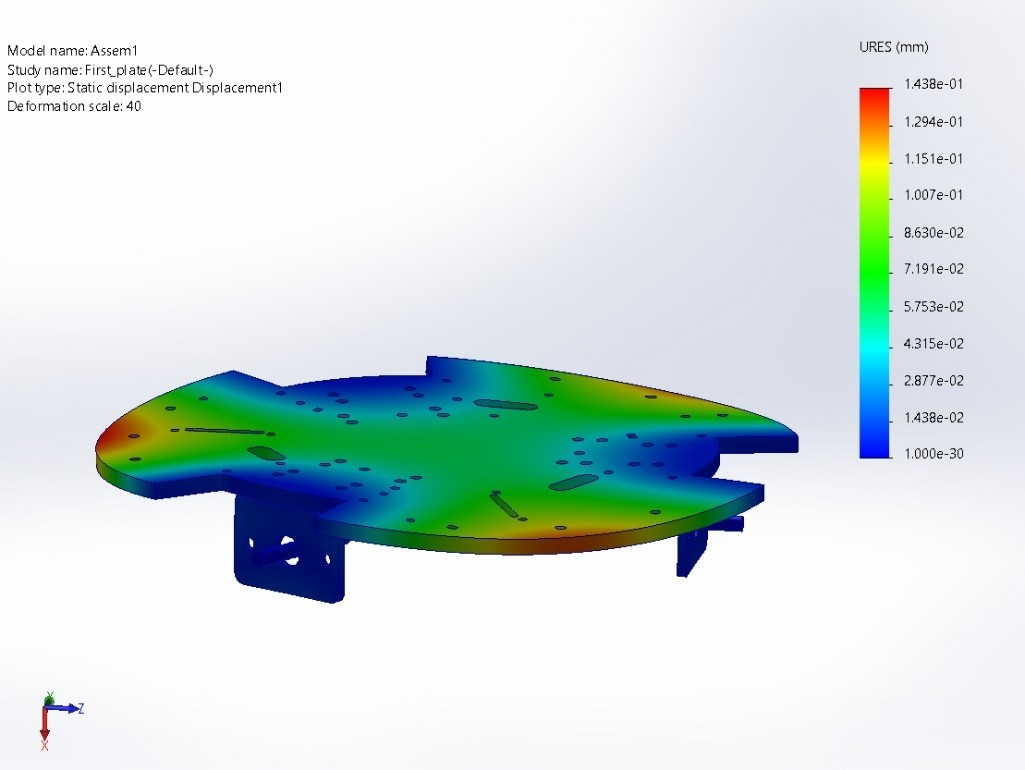
\includegraphics[width=0.75\linewidth]{figures/Chapter 3/Displacement6mm.jpg}
    \caption{Displacement (6mm)}
\end{figure}
\begin{figure}[H]
    \centering
    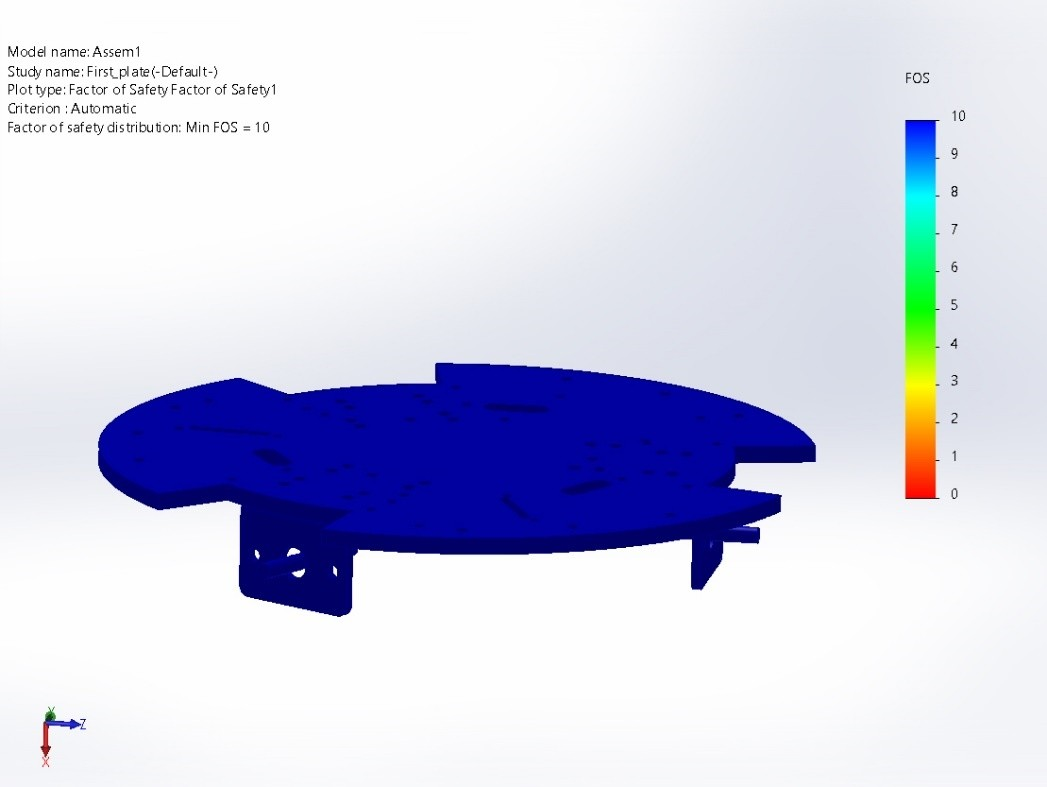
\includegraphics[width=\linewidth]{figures/Chapter 3/Safety_factor6mm.jpg}
    \caption{Safety Factor (6mm)}
\end{figure}

\subsubsection{Comparison Table}
\begin{table}[H]
\centering
\caption{Comparison of 3mm vs 6mm Acrylic}
\label{tab:acrylic_comparison}
\begin{tabular}{|l|c|c|}
\hline
\textbf{Metric} & \textbf{Acrylic Plate (3mm)} & \textbf{Acrylic Plate (6mm)} \\ \hline
Weight (gm) & 160 & 330 \\ \hline
Von Mises Stress (MPa) & 21 & 12 \\ \hline
Displacement (mm) & 0.7 & 0.145 \\ \hline
Safety Factor & 10 & 10 \\ \hline
\end{tabular}
\end{table}

Based on the Empirical Stress Analysis we conclude that the Acrylic of (6mm) thickness is the more effective thickness to be used as it’s Stronger, more durable and less in deflection in the plate to ensure the good motion of the robot without any vibrations and ensuring the wheel has more contact with the ground.


\newpage
\subsubsection{All Three layers Stress Analysis}
\begin{itemize}
    \item \textbf{Material:} Acrylic (medium-high impact)
    \item \textbf{Dimensions:} $\phi$260x6mm
    \item \textbf{Load:} 50 N
\end{itemize}
Specifying each weight of each component as a load on the point of fixation on the robot to get the more accurate results could be got.

\begin{figure}[H]
    \centering
    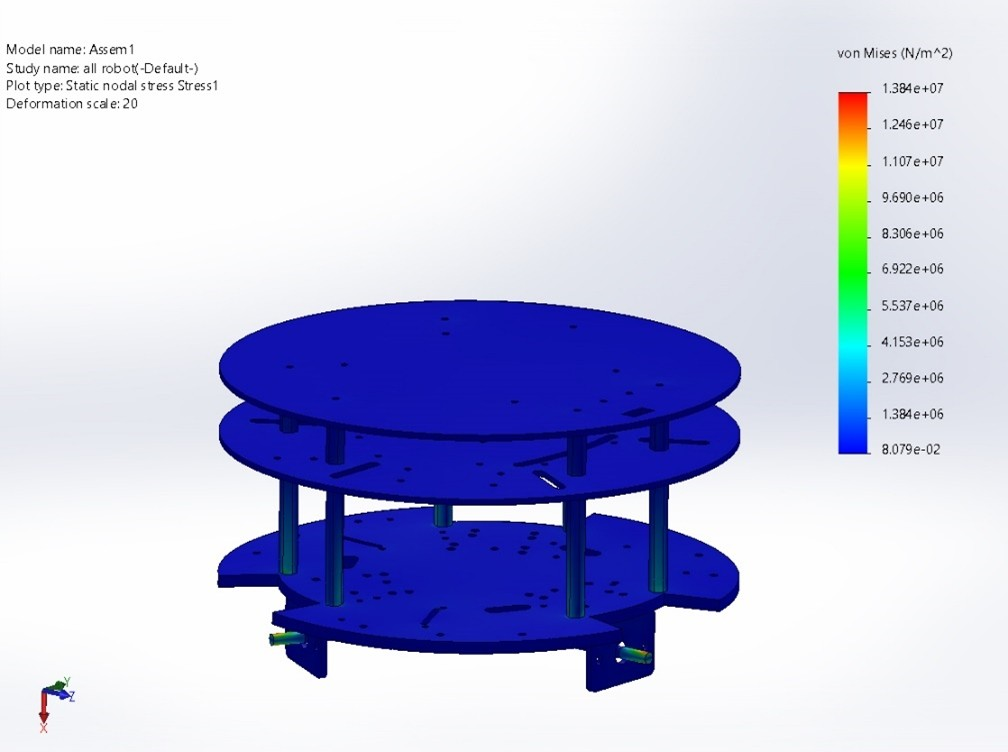
\includegraphics[width=\linewidth]{figures/Chapter 3/plate_assembly_Von_Mises_Stress.jpg}
    \caption{Full Assembly Von Mises Stress}
\end{figure}

\begin{figure}[H]
    \centering
    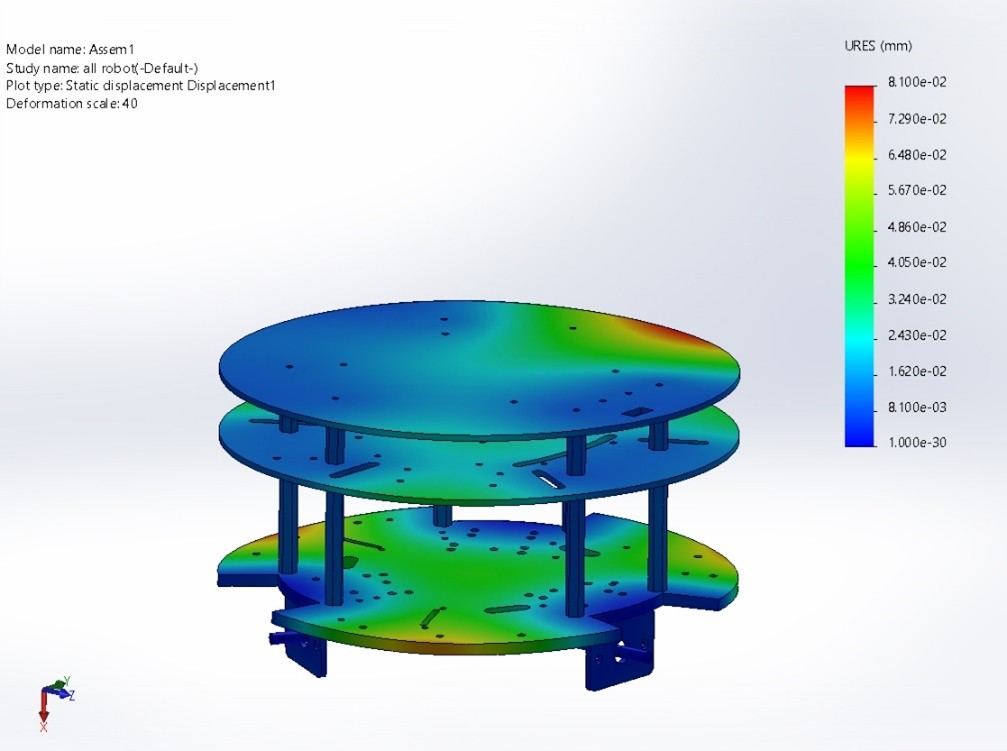
\includegraphics[width=0.7\linewidth]{figures/Chapter 3/plate_assembly_displacement.jpg}
    \caption{Full Assembly Displacement}
\end{figure}

\begin{figure}[H]
    \centering
    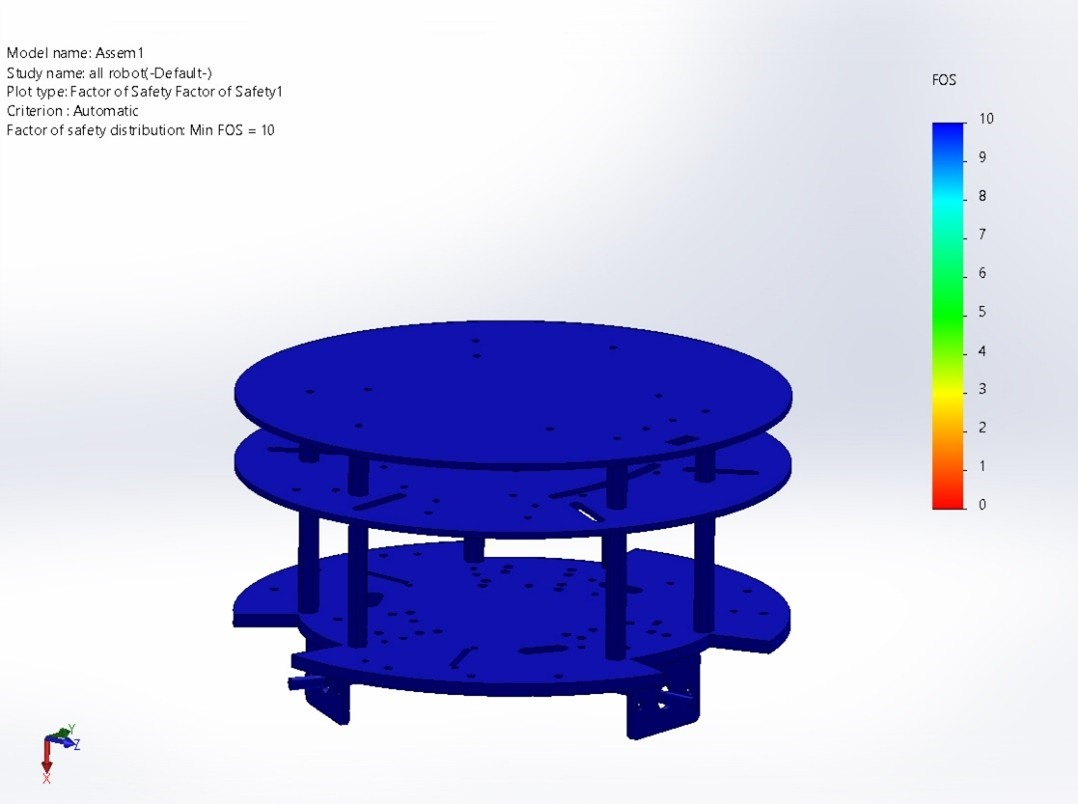
\includegraphics[width=0.7\linewidth]{figures/Chapter 3/plate_assembly_safety_factor.jpg}
    \caption{Full Assembly Safety Factor}
\end{figure}

The structural analysis confirms that the mechanical design is fully optimized for the project requirements. according to the results the chassis is durable enough to withstand more than it's designed for, ensuring minimal displacement to ensure that the kinematics of the 3-omni-wheel system remain accurate for odometry. In summary, the mechanical assembly is verified as safe, stable, and ready for manufacturing phase.

\section{Kinematic Modeling and URDF Generation}
\label{sec:urdf_generation}

The transition from a high-fidelity static SolidWorks assembly to a dynamic, simulation-ready robot is a defining phase in the development of the AUSRA swarm robots. In the context of modern mechatronics, the Unified Robot Description Format (URDF) serves as the ``single source of truth'' for the robot's physical properties, kinematic chains, and visual representation.

\subsection{Kinematic Tree Construction and Geometric Pre-processing}

The transformation of the CAD model into a functional URDF began within SolidWorks using the \texttt{sw2urdf} exporter plugin. However, for a 3-wheel omnidirectional drive, simply exporting the geometry is insufficient. To ensure the resulting model accurately reflected the physical constraints of the 120° radial symmetry, a rigorous pre-processing phase was conducted.

A robotic system is essentially a collection of ``Links'' (rigid bodies) connected by ``Joints'' (rotational or translational pivots). For the AUSRA robot, a hierarchical ``tree'' was established, starting with the \texttt{base\_link} as the root.

\begin{figure}[H]
    \centering
    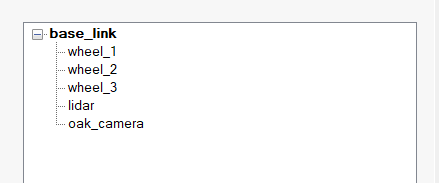
\includegraphics[width=0.85\textwidth]{figures/Chapter 5/Joints_solidworks.png}
    \caption{URDF Joint Definition in SolidWorks}
    \label{fig:joints_solidworks}
\end{figure}

To ensure precision of the kinematic transforms (TF), manual reference points were established at the geometric center of every motor shaft, wheel, and sensor. For each omni-wheel, a specific rotational axis was defined to pass through these points, serving as the pivot for the continuous joints.

A critical step was the creation of custom coordinate frames for each link, meticulously aligned such that the X, Y, and Z axes strictly adhered to the Denavit-Hartenberg (D-H) parameters. This manual alignment ensures that the ROS 2 TF tree correctly maps linear and angular velocities to the physical wheel orientations without geometric drift or mathematical singularities during runtime.

As shown in the URDF tree, the parent link specified was the \texttt{base\_link} which consists of the external body, the cover, and the base plate of the robot. The other links are all child links to the base link. Internal components not critical for simulation locomotion were omitted to keep the package lightweight for Gazebo simulation.

\begin{figure}[H]
    \centering
    \begin{subfigure}[b]{0.48\textwidth}
        \centering
        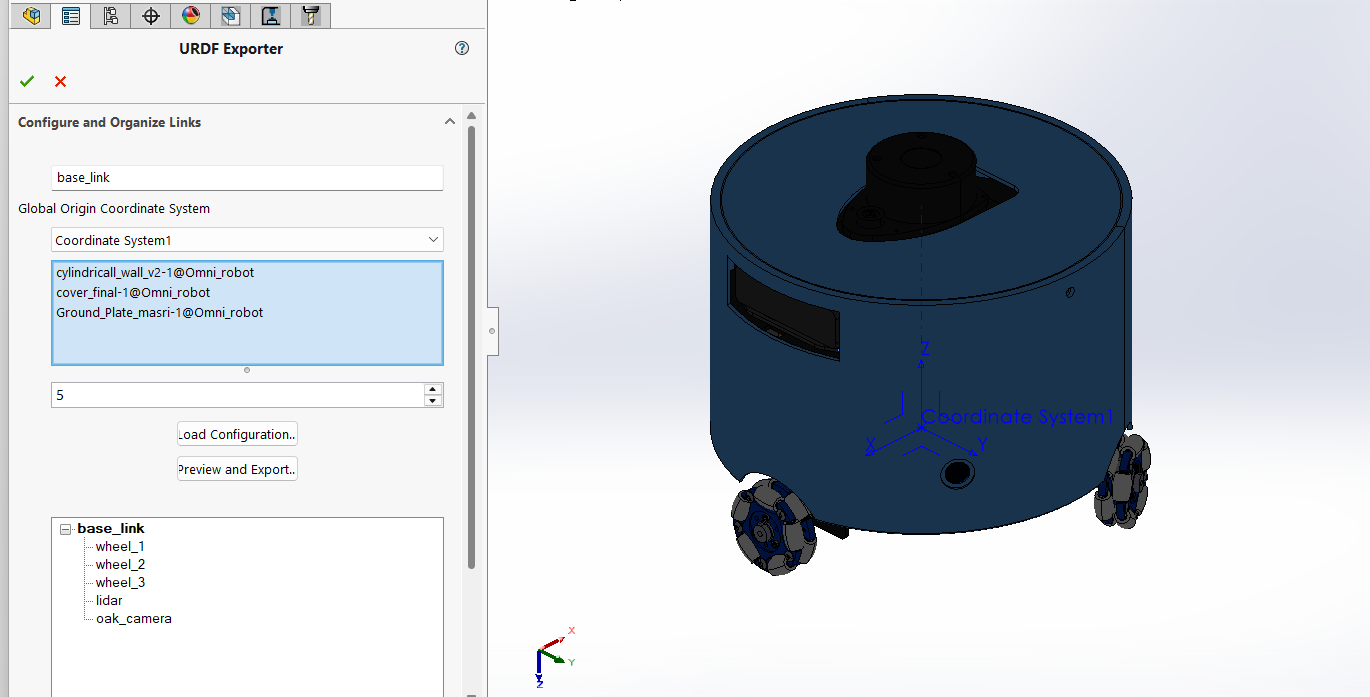
\includegraphics[width=\textwidth]{figures/Chapter 5/frames_gazebo_v1.png}
        \caption{Base Link Frame Definition}
        \label{fig:frames_gazebo_v1}
    \end{subfigure}
    \hfill
    \begin{subfigure}[b]{0.48\textwidth}
        \centering
        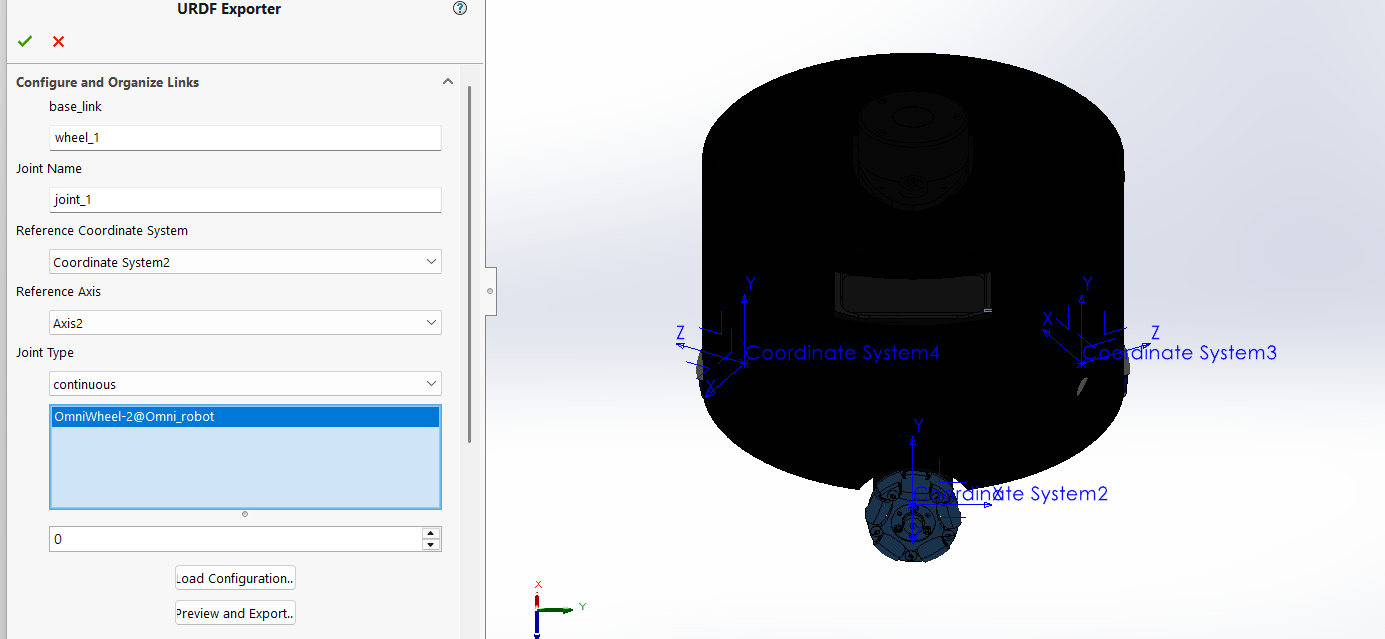
\includegraphics[width=\textwidth]{figures/Chapter 5/Frames_gazebo_v2.png}
        \caption{Wheel Frame Alignment}
        \label{fig:frames_gazebo_v2}
    \end{subfigure}
    \caption{Coordinate Frame Definition in Gazebo}
    \label{fig:frames_gazebo}
\end{figure}

For an omnidirectional platform, this alignment is vital; the Z-axis of each wheel must be perfectly perpendicular to the Z-axis of the \texttt{base\_link} coordinate frame and perpendicular to the wheel side face, while the X-axis must align with the forward translation vector of that specific wheel. Each wheel has its coordinate frame and axis specified with joint type set to \texttt{continuous}.

\begin{figure}[H]
    \centering
    \begin{subfigure}[b]{0.48\textwidth}
        \centering
        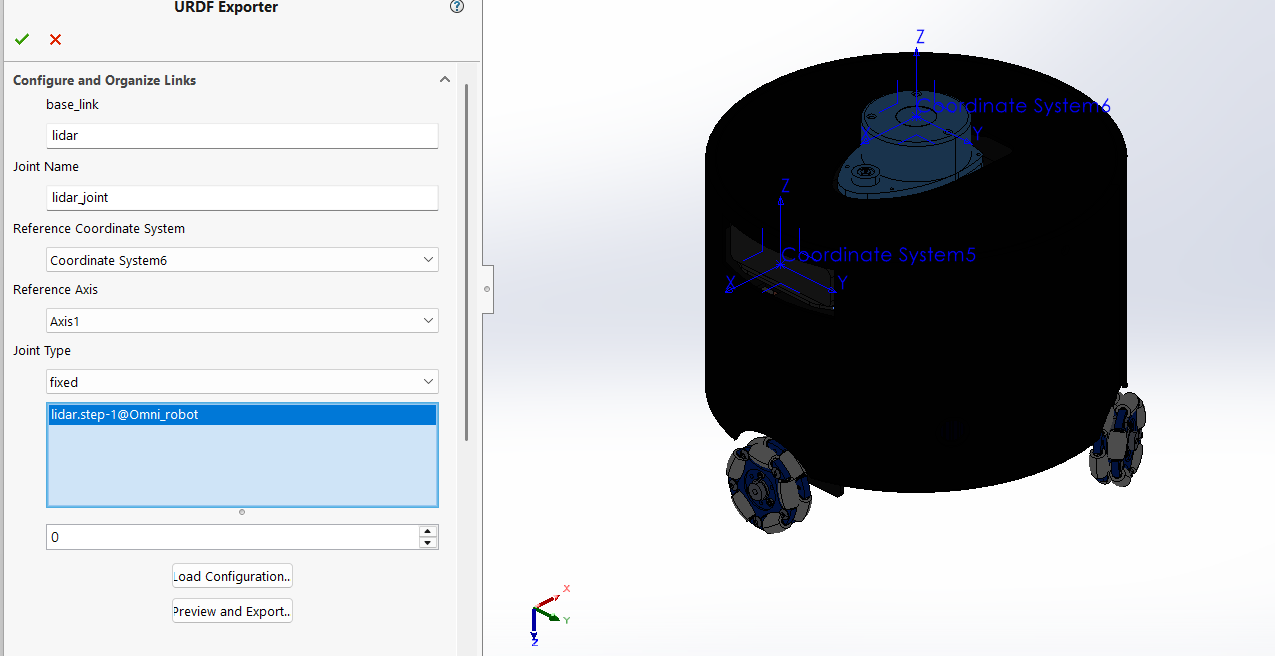
\includegraphics[width=\textwidth]{figures/Chapter 5/Frames_gazebo_v3.png}
        \caption{LiDAR and Camera Link Placement}
        \label{fig:frames_gazebo_v3}
    \end{subfigure}
    \hfill
    \begin{subfigure}[b]{0.48\textwidth}
        \centering
        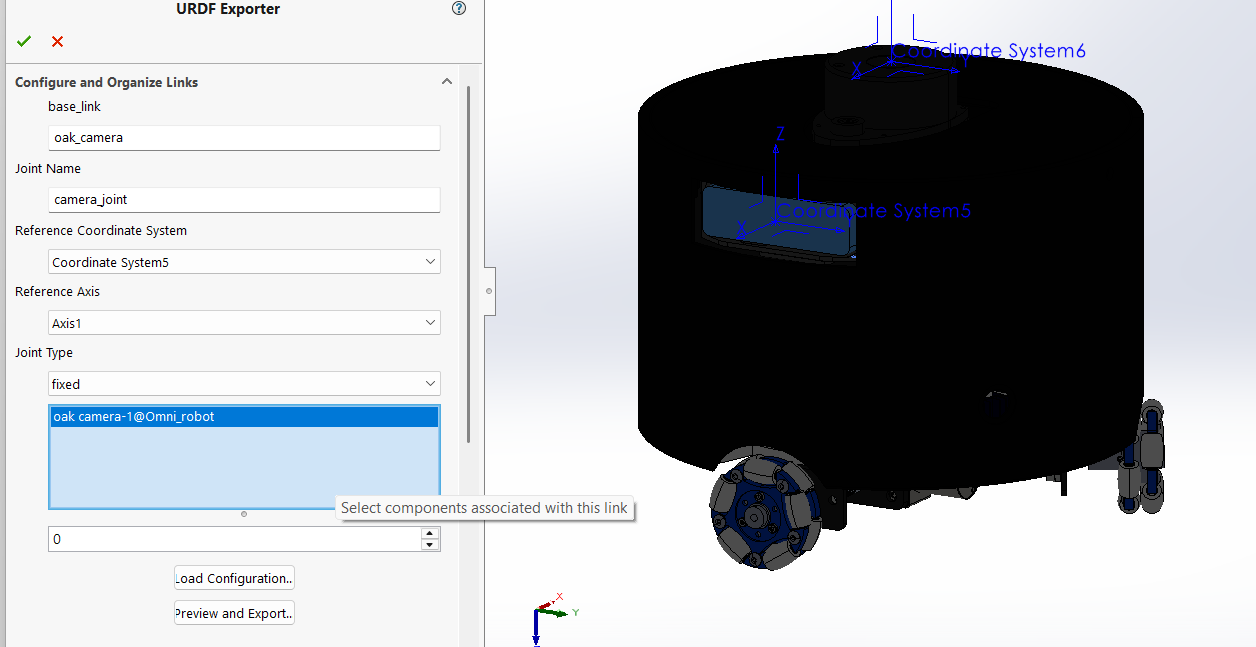
\includegraphics[width=\textwidth]{figures/Chapter 5/Frames_gazebo_v4.png}
        \caption{Complete TF Tree Visualization}
        \label{fig:frames_gazebo_v4}
    \end{subfigure}
    \caption{Sensor Link Definition}
    \label{fig:sensor_frames}
\end{figure}

The LiDAR link and OAK-D camera link are specified in the URDF for accurate placement when plugins are added for Gazebo simulation testing and code verification. The joint types of these sensor links are \texttt{fixed}.

\subsection{ROS 2 Migration and Package Reconfiguration}

Once the reference geometry and kinematic relationships were finalized, the robot was exported as a unified package. However, a significant technical hurdle was encountered: the standard exporter plugin is natively designed for the legacy ROS 1 environment. This resulted in a directory structure, metadata, and launch logic that were entirely incompatible with the ROS 2 Humble stack and its \texttt{ament\_cmake} build system.

To resolve this, a comprehensive reconfiguration of the exported package was undertaken:

\subsubsection{Build System Adaptation}

The \texttt{package.xml} was rewritten to include modern ROS 2 dependencies such as \texttt{robot\_state\_publisher}, \texttt{joint\_state\_publisher}, and \texttt{xacro}. Simultaneously, the \texttt{CMakeLists.txt} was reconstructed to utilize the \texttt{ament\_package()} macros, ensuring the meshes and URDF files were correctly indexed during the \texttt{colcon build} process.

\subsubsection{Launch System Development}

In ROS 2, launch files are Python-based scripts that manage the lifecycle and parameters of multiple nodes. New launch files were developed for two primary tasks:

\paragraph{RViz2 Visualization}
A launch script was created to load the URDF, start the \texttt{robot\_state\_publisher}, and open RViz2 with a pre-configured view. This allows real-time verification of the transform frames (TF), ensuring the OAK-D camera and LiDAR are spatially aligned with the robot's center.

\begin{figure}[H]
    \centering
    \begin{subfigure}[b]{0.48\textwidth}
        \centering
        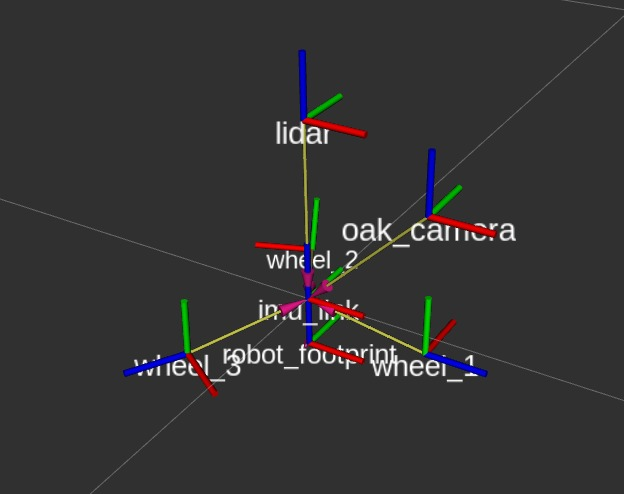
\includegraphics[width=\textwidth]{figures/Chapter 5/Frames_axis_rviz2.jpeg}
        \caption{TF Frames in RViz2}
        \label{fig:frames_rviz1}
    \end{subfigure}
    \hfill
    \begin{subfigure}[b]{0.48\textwidth}
        \centering
        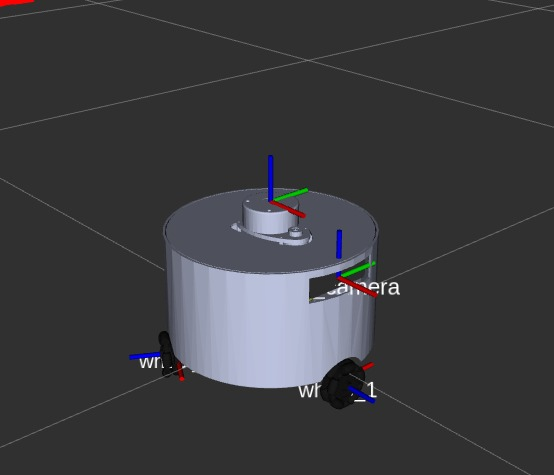
\includegraphics[width=\textwidth]{figures/Chapter 5/Frames_axis_rviz_1.jpeg}
        \caption{Robot Model Visualization}
        \label{fig:frames_rviz2}
    \end{subfigure}
    \caption{URDF Visualization in RViz2}
    \label{fig:rviz_visualization}
\end{figure}

\paragraph{Gazebo Simulation}
A secondary launch file was engineered to ``spawn'' the robot within the Gazebo physics engine. This required converting the URDF into an SDF (Simulation Description Format) on the fly and integrating Gazebo-specific plugins for the camera, IMU, LiDAR, and the omnidirectional wheel controller.

\begin{figure}[H]
    \centering
    \begin{subfigure}[b]{0.48\textwidth}
        \centering
        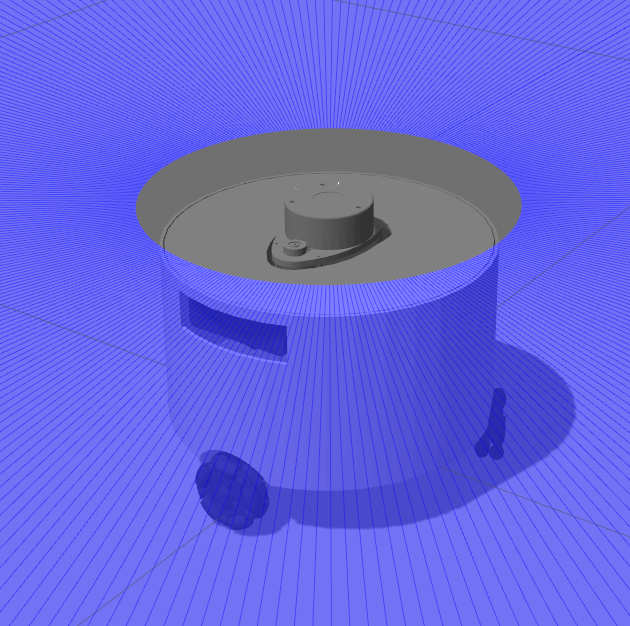
\includegraphics[width=\textwidth]{figures/Chapter 5/Robot_gazebo1.png}
        \caption{Robot Spawned in Gazebo}
        \label{fig:robot_gazebo1}
    \end{subfigure}
    \hfill
    \begin{subfigure}[b]{0.48\textwidth}
        \centering
        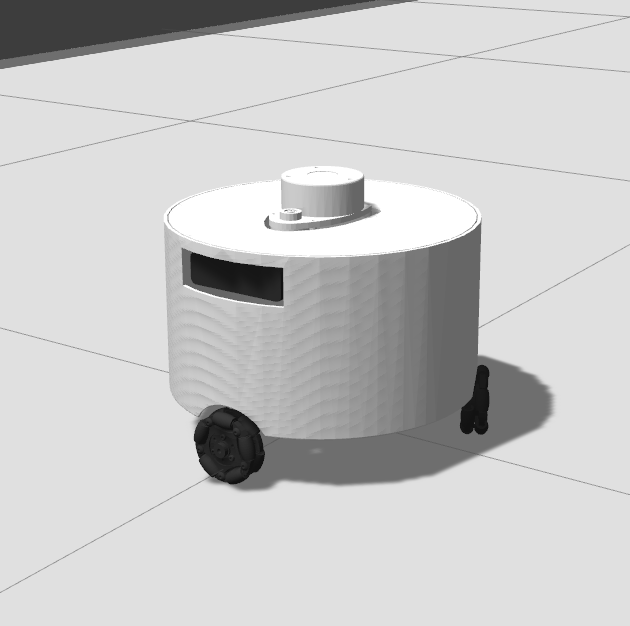
\includegraphics[width=\textwidth]{figures/Chapter 5/Robot_gazebo2.png}
        \caption{Physics Simulation Active}
        \label{fig:robot_gazebo2}
    \end{subfigure}
    \caption{AUSRA Robot in Gazebo Simulation}
    \label{fig:gazebo_simulation}
\end{figure}

\subsubsection{Inertial and Visual Optimization}

To ensure realistic behavior in simulation, the \texttt{<inertial>} tags for each link were populated using the exact mass and ``Inertia Tensor'' values calculated by SolidWorks' Mass Properties tool. Furthermore, the visual meshes were optimized and exported as \texttt{.stl} files, providing high-fidelity visual representation in RViz2 while maintaining low computational overhead.

\subsection{Summary}

The final result of this process is a robust and dynamic-ready model of the AUSRA robot that can be spawned in the Gazebo environment. This is the foundational step for any autonomous robot project. The reconfigured package serves as the bridge between the mechanical design and the high-level autonomous navigation algorithms, allowing the research team to test swarm coordination and SLAM algorithms in a high-fidelity simulation environment before deploying the physical robots---significantly reducing the risk of hardware damage during the development of complex 2D mapping behaviors.

% ============================================================================
% Chapter 4: Electrical System Architecture and Embedded Design
% ============================================================================

\chapter{Electrical System Architecture and Embedded Design}
\label{chap:electrical}

\section{Overview}
\label{sec:electrical_overview}

This chapter details the design, implementation, and integration of the electrical subsystems for the AUSRA mobile robot platform. The electrical architecture is designed to support a robust, autonomous swarm capability by prioritizing three key engineering principles:

\begin{enumerate}
    \item \textbf{Hierarchical Control:} Decoupling high-level AI processing from low-level real-time actuation ensures that computationally intensive tasks such as SLAM and path planning do not interfere with time-critical motor control loops.
    \item \textbf{Power Isolation:} Separating noisy motor loads from sensitive logic circuits prevents electromagnetic interference and voltage fluctuations from corrupting sensor data or causing computational errors.
    \item \textbf{Modular Safety:} Implementing physical hardware failsafes for charging and operation protects both the user and the electronic components from hazardous conditions.
\end{enumerate}

\section{System Topology}
\label{sec:system_topology}

The system is built upon a distributed power and control architecture. A central 20V DC bus, derived from a high-discharge Lithium-Ion source, powers two distinct regulation stages: the \textbf{Logic Stage} for computation and sensors, and the \textbf{Actuation Stage} for motor propulsion.

The control hierarchy consists of an NVIDIA Jetson Orin Nano serving as the high-level ``Brain'' (handling SLAM, path planning, and vision), which communicates via serial interface with an ESP32 Microcontroller, acting as the low-level ``Spine'' (handling inverse kinematics, PID control, and IMU data acquisition).

\begin{figure}[H]
    \centering
    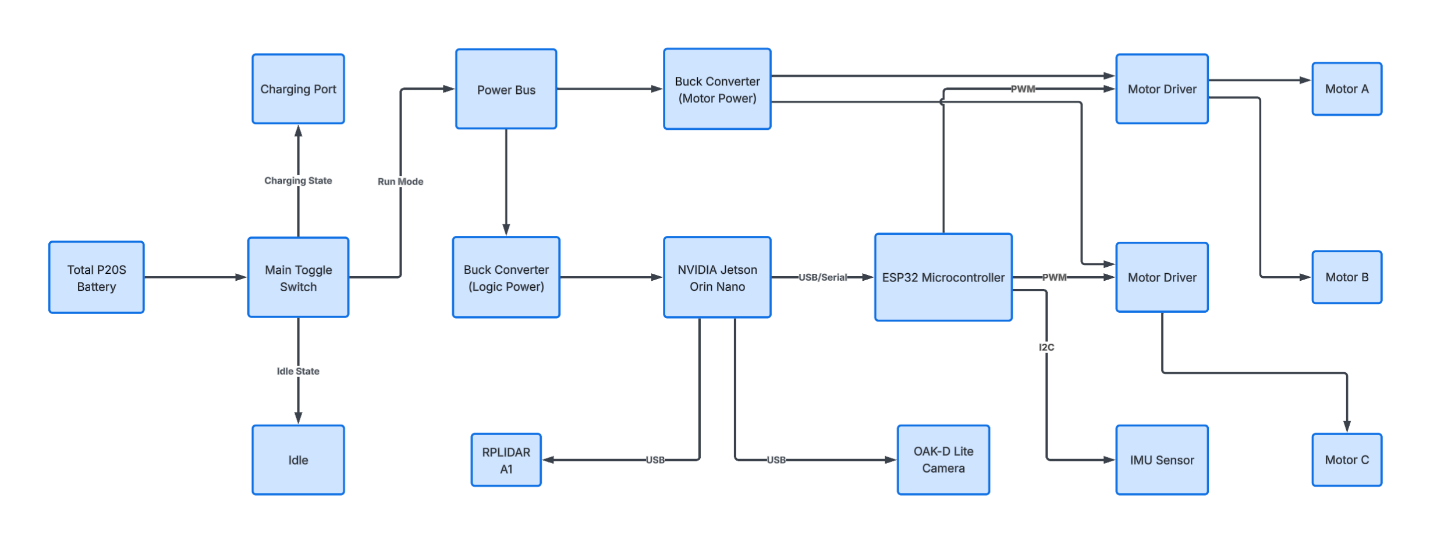
\includegraphics[width=0.85\linewidth]{figures/Chapter 4/System_topology.png}
    \caption{Electrical System Topology showing the hierarchical control architecture}
    \label{fig:system_topology}
\end{figure}

\section{Component Selection and Justification}
\label{sec:component_selection}

The selection of hardware components was driven by the specific requirements of holonomic motion and edge-AI processing. Each component underwent rigorous evaluation using weighted decision matrices to ensure optimal performance within the project constraints.

\subsection{Low-Level Controller Selection}
\label{subsec:lowlevel_controller}

The selection of the low-level microcontroller was critical for ensuring reliable real-time motor control and seamless communication with the high-level ROS 2 stack. Three candidates were evaluated: \textbf{Teensy 4.1}, \textbf{STM32F411}, and \textbf{ESP32-S3}.

\subsubsection{Selection Criteria}

\begin{enumerate}
    \item \textbf{Micro-ROS Compatibility:} The ability to run micro-ROS agents natively for seamless node integration with the ROS 2 ecosystem \cite{microros2023}.
    \item \textbf{Ease of Development:} The learning curve required to implement drivers; specifically comparing the Arduino ecosystem against vendor-specific HALs (Hardware Abstraction Layers).
    \item \textbf{Memory \& Performance:} SRAM size for buffering ROS messages and clock speed for executing PID loops at high frequency.
    \item \textbf{Cost:} Unit cost per board, which scales significantly across a swarm deployment.
\end{enumerate}

\subsubsection{Selection Matrix}

\begin{table}[H]
\centering
\caption{Microcontroller Weighted Decision Matrix (Scale: 1 = Poor, 10 = Excellent)}
\label{tab:mcu_selection}
\begin{tabular}{|l|c|c|c|c|}
\hline
\textbf{Criteria} & \textbf{Weight} & \textbf{Teensy 4.1} & \textbf{STM32F411} & \textbf{ESP32-S3} \\ \hline
Micro-ROS Support & 0.30 & 8 & 6 & 10 \\ \hline
Ease of Use & 0.25 & 10 & 5 & 9 \\ \hline
Memory / Specs & 0.25 & 10 & 6 & 7 \\ \hline
Cost Efficiency & 0.20 & 3 & 10 & 9 \\ \hline
\textbf{Weighted Score} & \textbf{1.00} & \textbf{7.95} & \textbf{6.55} & \textbf{8.80} \\ \hline
\end{tabular}
\end{table}

\begin{figure}[H]
    \centering
    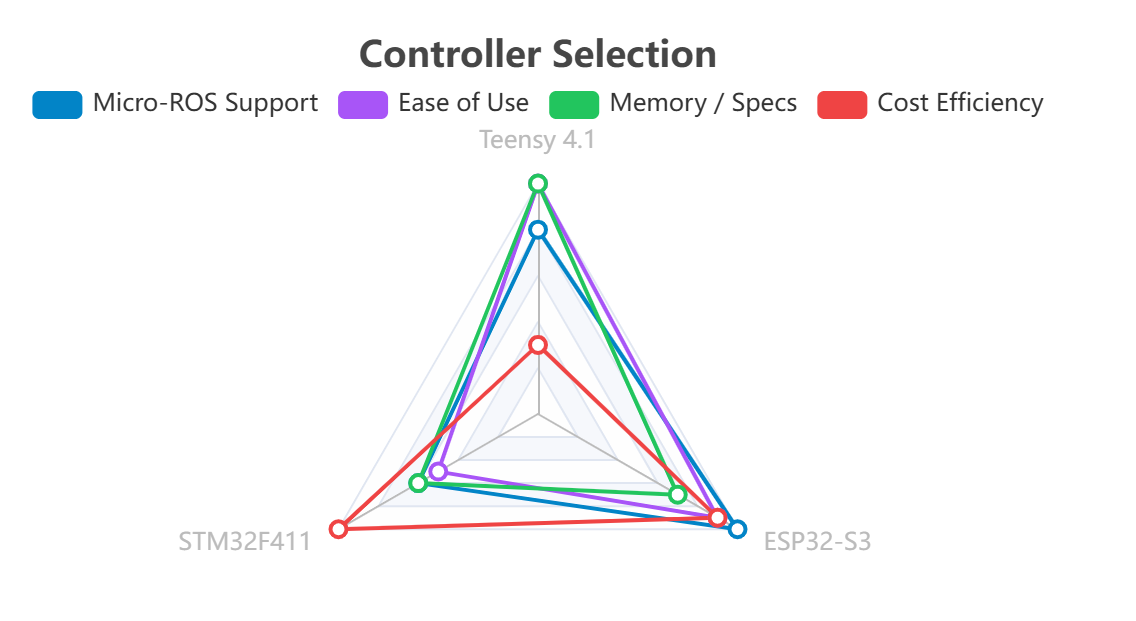
\includegraphics[width=0.7\linewidth]{figures/Chapter 4/Control_selection.png}
    \caption{Microcontroller Selection Comparison}
    \label{fig:control_selection}
\end{figure}

\newpage
\subsubsection{Summary of Microcontroller Selection}

\begin{figure}[H]
    \centering
    \begin{subfigure}[b]{0.3\textwidth}
        \centering
        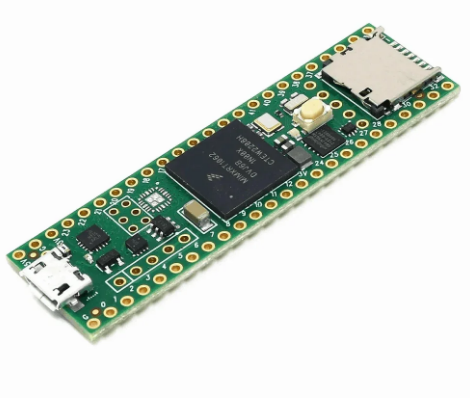
\includegraphics[width=\linewidth]{figures/Chapter 4/Teensy4_1.png}
        \caption{Teensy 4.1}
        \label{fig:teensy}
    \end{subfigure}
    \hfill
    \begin{subfigure}[b]{0.3\textwidth}
        \centering
        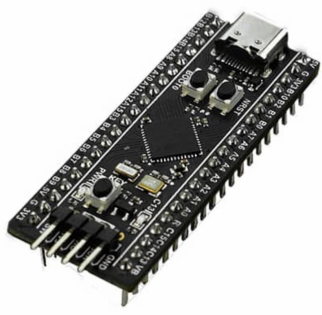
\includegraphics[width=\linewidth]{figures/Chapter 4/STM32F411.png}
        \caption{STM32F411}
        \label{fig:stm32}
    \end{subfigure}
    \hfill
    \begin{subfigure}[b]{0.3\textwidth}
        \centering
        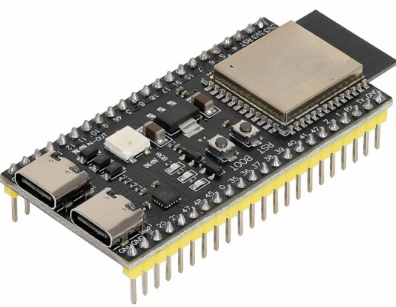
\includegraphics[width=\linewidth]{figures/Chapter 4/Esp32-s3.png}
        \caption{ESP32-S3 (Selected)}
        \label{fig:esp32}
    \end{subfigure}
    \caption{Microcontroller Candidates Evaluated}
    \label{fig:mcu_candidates}
\end{figure}

\paragraph{Teensy 4.1 (Score: 7.95/10)}
The Teensy 4.1 demonstrated superior raw computational performance, achieving a perfect score in technical specifications due to its 600 MHz Cortex-M7 processor. While this processing power offers significant headroom for complex kinematics, the platform's high unit cost (\textasciitilde\$30) resulted in a poor cost-efficiency rating. For a scalable swarm robotics architecture where per-unit cost is a critical constraint, the Teensy 4.1 presented a diminishing return on investment, as its surplus processing power exceeded the requirements of the low-level control loop.

\paragraph{STM32F411 (Score: 6.55/10)}
The STM32F411 ``Black Pill'' represents the industry-standard solution for embedded control, securing a perfect score for cost efficiency (\textasciitilde\$6). However, its integration into the AUSRA architecture was penalized by significant development overhead. The STM32 ecosystem (HAL/Cube IDE) requires a steeper learning curve compared to the Arduino framework, and the lack of native wireless connectivity necessitates an external bridge for micro-ROS communication. These factors would have introduced unacceptable latency into the development timeline without offering a distinct advantage in motor control precision.

\paragraph{ESP32-S3 (Selected --- Score: 8.80/10)}
The ESP32-S3 was identified as the optimal solution, balancing cost, performance, and connectivity \cite{espressif2023esp32}. Although its clock speed is lower than the Teensy, its \textbf{Dual-Core Xtensa LX7 architecture} provides a unique architectural advantage---it allows for the dedicated separation of tasks, with one core handling the blocking micro-ROS communication stack and the second core executing real-time motor control interrupts. Furthermore, its native support for Wi-Fi and USB-OTG simplified the hardware topology by eliminating the need for external communication bridges, justifying its selection as the primary low-level controller.

\newpage
\subsection{Motor Driver Selection}
\label{subsec:motor_driver}

The motor driver selection is critical for swarm robot efficiency, as the system operates on finite battery capacity and must maintain a compact form factor. The driver must offer high power efficiency and an optimal power-to-weight ratio.

\subsubsection{Candidates Evaluated}

Two motor driver families were evaluated:
\begin{itemize}
    \item \textbf{L298N:} A classic bipolar-transistor-based driver, widely available and popular for hobbyist applications.
    \item \textbf{Cytron MDD3A/MDD10A:} Modern MOSFET-based drivers offering superior efficiency and thermal performance.
\end{itemize}

\subsubsection{Selection Matrix}

\begin{table}[H]
\centering
\caption{Motor Driver Selection Matrix}
\label{tab:motor_driver_selection}
\resizebox{\textwidth}{!}{%
\begin{tabular}{|l|c|c|c|c|c|c|c|}
\hline
\multirow{2}{*}{\textbf{Criteria}} & \multirow{2}{*}{\textbf{Weight}} & \multicolumn{2}{c|}{\textbf{L298N}} & \multicolumn{2}{c|}{\textbf{Cytron MDD3A}} & \multicolumn{2}{c|}{\textbf{Cytron MDD10A}} \\ \cline{3-8} 
 & & Rating/5 & Score & Rating/5 & Score & Rating/5 & Score \\ \hline
Efficiency (Voltage drop) & 5 & 2 & 10 & 4 & 20 & 4 & 20 \\ \hline
Current Capacity & 4 & 3 & 12 & 4 & 16 & 5 & 20 \\ \hline
Price & 3 & 5 & 15 & 4 & 12 & 2 & 6 \\ \hline
Size \& Weight & 3 & 5 & 15 & 5 & 15 & 3 & 9 \\ \hline
\textbf{Final Scores} &  &  & \textbf{52} &  & \textbf{63} &  & \textbf{55} \\ \hline
\end{tabular}%
}
\end{table}

\subsubsection{Final Selection: Cytron MDD3A}

The \textbf{Cytron MDD3A} (Dual Channel 3A Motor Driver) was selected. The MDD10A's 10A rating was excessive for the selected actuators (stall current $<$2.5A), and each robot requires two drivers for three motors.

\begin{figure}[H]
    \centering
    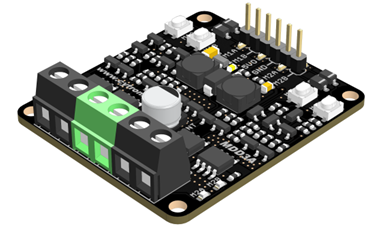
\includegraphics[width=0.4\linewidth]{figures/Chapter 4/MDD3A_Motor_Driver_2_Channel.png}
    \caption{Cytron MDD3A Dual Channel Motor Driver}
    \label{fig:mdd3a}
\end{figure}

\subsubsection{Justification of Selection}

\paragraph{Current Headroom}
The L298N (2.0A continuous) would operate at 90\% capacity with motors drawing 1.5--1.8A, risking overheating. The MDD3A (3.0A continuous, 5.0A peak) provides a 50\% safety margin.

\paragraph{Thermal Efficiency}
The L298N's BJT technology suffers from $\approx$2V voltage drop, wasting 17\% of power as heat on a 12V rail. The MDD3A's MOSFET technology ($R_{DS(on)} < 0.1\Omega$) delivers virtually all power to the motors, extending battery life and eliminating bulky heatsinks.

\paragraph{Protection Features}
The MDD3A includes active dynamic braking and fast-response protection circuits for precise stopping---essential for collision avoidance in swarm applications.

\paragraph{Size Optimization}
The MDD3A is 60\% smaller than the MDD10A, enabling a more compact chassis design and reduced weight.

\subsection{Power Source Selection}
\label{subsec:power_source}

\subsubsection{Design Constraint}
The primary power requirement was dictated by the NVIDIA Jetson Orin Nano, which operates most efficiently at higher input voltages ($>$12V) to minimize current draw and thermal dissipation. The local market availability in Egypt limited standard RC LiPo packs primarily to 3S (11.1V) configurations, which fall below the optimal efficiency threshold for the compute stack.

\subsubsection{Candidates Evaluated}

\begin{enumerate}
    \item \textbf{Single 3S LiPo (11.1V):} The standard hobbyist solution.
    \item \textbf{Dual 3S LiPo in Series (6S / 22.2V):} Connecting two packs to double the voltage.
    \item \textbf{Total P20S Industrial Pack (20V):} A commercial off-the-shelf power tool battery.
\end{enumerate}

\begin{figure}[H]
    \centering
    \begin{subfigure}[b]{0.45\textwidth}
        \centering
        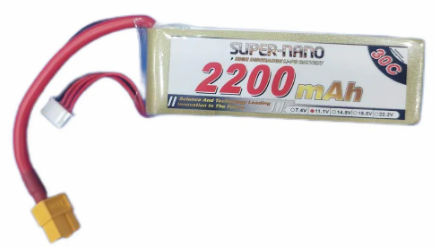
\includegraphics[width=\linewidth]{figures/Chapter 4/3S_Battery.png}
        \caption{Standard 3S LiPo Battery}
        \label{fig:3s_battery}
    \end{subfigure}
    \hfill
    \begin{subfigure}[b]{0.45\textwidth}
        \centering
        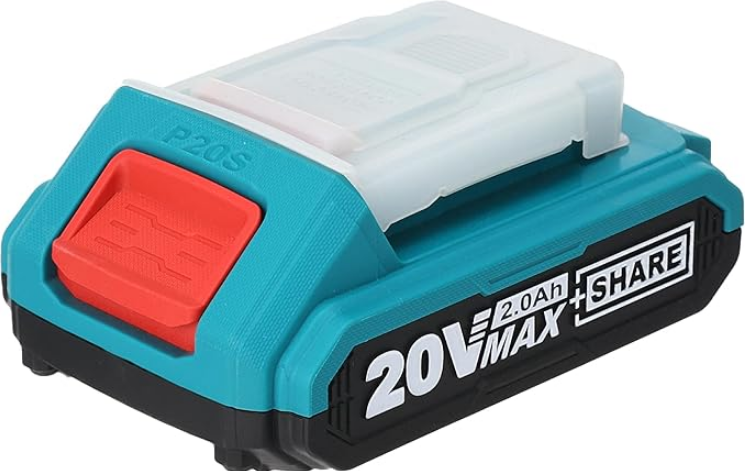
\includegraphics[width=\linewidth]{figures/Chapter 4/Total_p20s_battery.png}
        \caption{Total P20S Industrial Battery}
        \label{fig:p20s_battery}
    \end{subfigure}
    \caption{Power Source Candidates}
    \label{fig:battery_candidates}
\end{figure}

\subsubsection{Selection Matrix}

\begin{table}[H]
\centering
\caption{Power Source Comparison Matrix (Scale: 1 = Poor, 10 = Excellent)}
\label{tab:power_source_selection}
\begin{tabular}{|l|c|c|c|c|}
\hline
\textbf{Criteria} & \textbf{Weight} & \textbf{Single 3S LiPo} & \textbf{Dual 3S (Series)} & \textbf{Total P20S} \\ \hline
Voltage Sufficiency & 0.35 & 3 & 10 & 10 \\ \hline
Safety \& BMS & 0.25 & 6 & 2 & 10 \\ \hline
Charging Usability & 0.25 & 5 & 2 & 9 \\ \hline
Cost Efficiency & 0.15 & 8 & 4 & 9 \\ \hline
\textbf{Weighted Score} & \textbf{1.00} & \textbf{5.0} & \textbf{5.1} & \textbf{9.6} \\ \hline
\end{tabular}
\end{table}

\begin{figure}[H]
    \centering
    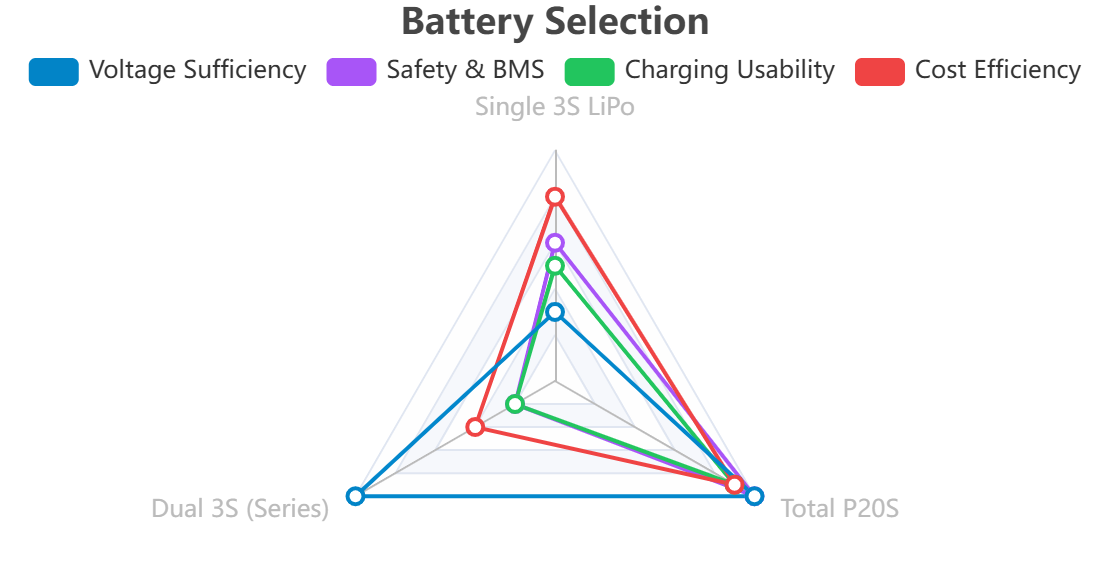
\includegraphics[width=0.7\linewidth]{figures/Chapter 4/Battery_selection.png}
    \caption{Battery Selection Comparison}
    \label{fig:battery_selection}
\end{figure}

\subsubsection{Justification of Selection}

\paragraph{Rejection of LiPo Configurations}
\begin{itemize}
    \item \textbf{Single 3S (11.1V):} Rejected as the nominal voltage (11.1V) forces the Jetson's internal regulators to draw higher current to maintain its power budget. This increases thermal stress and risks ``brownouts'' (voltage dips) when motors accelerate.
    \item \textbf{Dual Series (6S):} While a series configuration solves the voltage issue, it introduces significant safety and maintenance risks. Without a sophisticated industrial-grade BMS, two separate packs often discharge at uneven rates. This creates a scenario where one pack could drop below its critical voltage threshold while the other remains charged, leading to potential cell damage or fire hazards. Furthermore, the operational complexity of removing and balancing two separate packs for every charging cycle was deemed impractical for a user-friendly system.
\end{itemize}

\newpage
\paragraph{Selection of Total P20S (20V Platform)}
\begin{itemize}
    \item \textbf{Integrated BMS:} The battery features an internal Battery Management System that balances cells automatically, preventing the dangerous discharge scenarios inherent in custom series-LiPo setups.
    \item \textbf{Voltage Headroom:} The 20V nominal output ensures the Jetson and Motor Drivers operate in their high-efficiency capability region, significantly reducing amperage draw across the main bus.
    \item \textbf{``Charge-in-Place'' Architecture:} Unlike LiPos which require removal for safety, the P20S's ruggedized hard-shell casing and internal protections allowed us to design the ``Charging Mode'' circuit (referenced in Section \ref{subsec:isolation_logic}). This enables the robot to be charged safely via an external port without disassembling the chassis, mimicking commercial AMR (Autonomous Mobile Robot) standards.
\end{itemize}

\subsubsection{Battery Sizing (Target: $>$30 minutes runtime)}

\paragraph{Power Calculation}
The total power consumption was calculated by summing all major subsystems:

\begin{equation}
P_{total} = P_{Jetson} + P_{Motors} + P_{Camera} + P_{LiDAR} + P_{LowLevel}
\end{equation}

\begin{figure}[H]
    \centering
    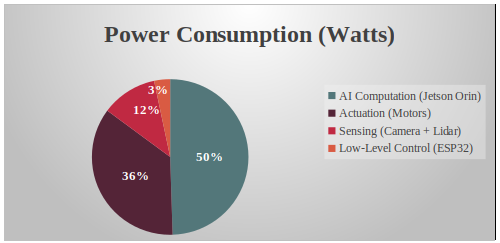
\includegraphics[width=0.6\linewidth]{figures/Chapter 4/Power_consumption.png}
    \caption{Power Consumption Breakdown}
    \label{fig:power_consumption}
\end{figure}

\textbf{Average Power:}
\begin{equation}
P_{avg} = 15 + 10.8 + 3 + 0.5 + 1 = 30.3 \approx 30 \text{ W}
\end{equation}

\textbf{Maximum Power:}
\begin{equation}
P_{max} = 25 + 72 + 5 + 1 + 1 = 104 \approx 105 \text{ W}
\end{equation}

\paragraph{Current Calculation}
Since the system is powered by a 20V source through Buck Converters, we calculate the current drawn from the battery, accounting for an estimated 90\% converter efficiency ($\eta = 0.9$).

\textbf{Average Current Draw:}
\begin{equation}
P_{batt,avg} = \frac{P_{avg}}{\eta} = \frac{30 \text{ W}}{0.9} = 33.3 \text{ W}
\end{equation}
\begin{equation}
I_{avg} = \frac{P_{batt,avg}}{V} = \frac{33.3 \text{ W}}{20 \text{ V}} = 1.67 \text{ A}
\end{equation}

\textbf{Peak Current Draw:}
\begin{equation}
P_{batt,max} = \frac{P_{max}}{\eta} = \frac{105 \text{ W}}{0.9} = 116.7 \text{ W}
\end{equation}
\begin{equation}
I_{max} = \frac{P_{batt,max}}{V} = \frac{116.7 \text{ W}}{20 \text{ V}} = 5.84 \text{ A}
\end{equation}

\paragraph{Capacity \& Runtime Verification}

\textbf{Selected Battery Specifications:}
\begin{itemize}
    \item \textbf{Model:} Total P20S (Lithium-Ion Power Tool Pack)
    \item \textbf{Voltage:} 20 V
    \item \textbf{Capacity:} 2000 mAh (2.0 Ah)
    \item \textbf{Discharge Rating:} High-Drain ($>$10C)
\end{itemize}

\textbf{Runtime Calculation:}
\begin{equation}
\text{Runtime} = \frac{\text{Capacity}}{I_{avg}} = \frac{2.0 \text{ Ah}}{1.67 \text{ A}} = 1.2 \text{ h} \approx 72 \text{ minutes}
\end{equation}

\textbf{Result:} The 2000mAh pack provides approximately 72 minutes of continuous operation, exceeding the 30-minute requirement by a factor of 2.4.

\paragraph{C-Rating (Discharge Safety) Check}
We must ensure the battery can handle the peak current (during acceleration/stall conditions) without damage.

\textbf{Required C-Rating:}
\begin{equation}
C_{req} = \frac{I_{max}}{\text{Capacity}} = \frac{5.84 \text{ A}}{2.0 \text{ Ah}} = 2.92 \text{ C}
\end{equation}

\textbf{Conclusion:} The required 2.92C is extremely low compared to the battery's rated capability ($>$10C), ensuring the pack will run cool and safe even during aggressive maneuvering.


\newpage
\section{Power Distribution and Safety Strategy}
\label{sec:power_distribution}

Effective power management is achieved through a combination of physical signal isolation and multi-stage voltage regulation.

\subsection{Physical Isolation Logic (Three-State Failsafe)}
\label{subsec:isolation_logic}

Safety is enforced via a \textbf{6-pin E-TEN1322 Toggle Switch (ON-OFF-ON)}. This component acts as a hardware multiplexer, defining three mutually exclusive operational states to prevent user error and electrical hazards.

\begin{figure}[H]
    \centering
    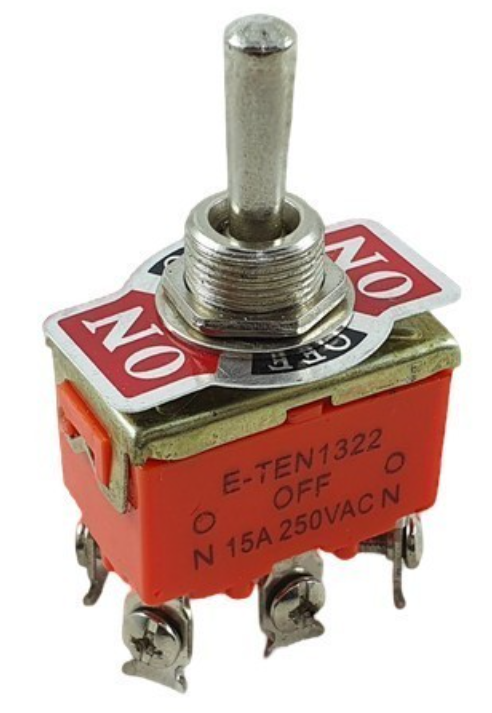
\includegraphics[width=0.3\linewidth]{figures/Chapter 4/Power_switch.png}
    \caption{Three-State Power Switch Configuration}
    \label{fig:power_switch}
\end{figure}

\begin{itemize}
    \item \textbf{State 1: Charge Mode} --- The battery terminals are electrically disconnected from the robot's internal power bus and routed exclusively to the external GX16 Aviation Port. This ensures 100\% isolation of the sensitive computing units (Jetson/ESP32) from potential voltage spikes or ground loops during the charging cycle.
    
    \item \textbf{State 2: Idle} --- In the neutral position, the battery is fully disconnected from both the charging port and the internal system. This serves as a \textbf{Master Kill Switch}, preventing accidental startup during transport, maintenance, or code flashing. It also mitigates parasitic battery drain when the robot is in storage.
    
    \item \textbf{State 3: Run Mode} --- The charging port is physically disconnected, and the battery power is routed to the internal 20V DC Bus. This activates the dual-stage regulation system to power the robot's logic and actuation subsystems.
\end{itemize}

\subsection{Dual-Stage Voltage Regulation}
\label{subsec:voltage_regulation}

To maintain system stability and component safety, the 20V bus is conditioned by two independent regulation stages:

\begin{figure}[H]
    \centering
    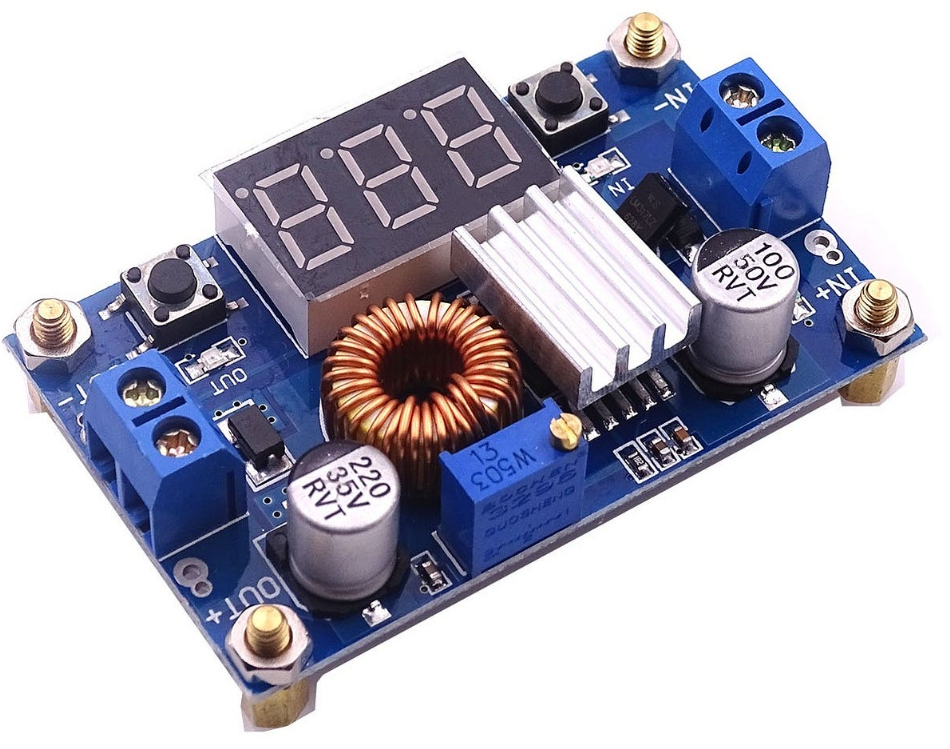
\includegraphics[width=0.7\linewidth]{figures/Chapter 4/Buck_convertor.png}
    \caption{Buck Converter Modules for Voltage Regulation}
    \label{fig:buck_converter}
\end{figure}

\begin{itemize}
    \item \textbf{Logic Regulator:} A precision step-down converter provides a stable supply for the NVIDIA Jetson Orin Nano. This isolation protects the compute stack from voltage ``brownouts'' that occur on the main line when motors draw high inrush currents during acceleration.
    
    \item \textbf{Actuation Regulator:} A dedicated high-power buck converter steps the 20V battery voltage down to a regulated 12V supply, matching the nominal voltage rating of the DC motors. This regulation guarantees that the motors receive a consistent voltage regardless of the battery's fluctuating charge level (21V to 18V), ensuring predictable kinematic performance throughout the entire discharge cycle.
\end{itemize}


\newpage
\section{Low-Level Firmware Design}
\label{sec:lowlevel_design}

This section presents the theoretical foundation and implementation strategy for the low-level motor control firmware running on the ESP32-S3 microcontroller.

\subsection{Actuator Feedback: Quadrature Encoders}
\label{subsec:encoders}

Encoders are sensors mounted on a motor's rear shaft to sense rotation. As the shaft moves, the encoder generates a pulse train signal that provides position and velocity feedback for closed-loop control.

\begin{figure}[H]
    \centering
    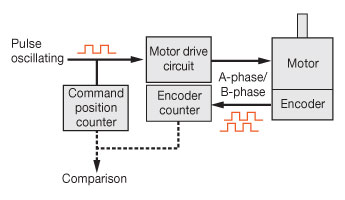
\includegraphics[width=0.6\linewidth]{figures/Chapter 4/Motor_encoder_topology.jpg}
    \caption{Motor Encoder Topology}
    \label{fig:encoder_topology}
\end{figure}

\subsubsection{Operating Principle}

The number of pulses indicates the motor shaft position and rotation distance from a home position. For example, with an encoder resolution of 935 PPR (Pulses Per Revolution), 935 pulses indicate one complete revolution. The pulse frequency (Hz) indicates rotational speed, while the phase relationship between channels A and B determines direction.

\paragraph{Optical Encoder Technology}
The AUSRA platform uses optical encoders, which provide the highest precision and resolution. In a transmissive optical encoder, the main components are:
\begin{itemize}
    \item A light emitter (LED)
    \item A code wheel with precision slits
    \item A light receiver (photo sensor)
\end{itemize}

As the code wheel rotates, light either passes through the slits or is blocked, creating a binary pulse train that the microcontroller interprets as position data.

\begin{figure}[H]
    \centering
    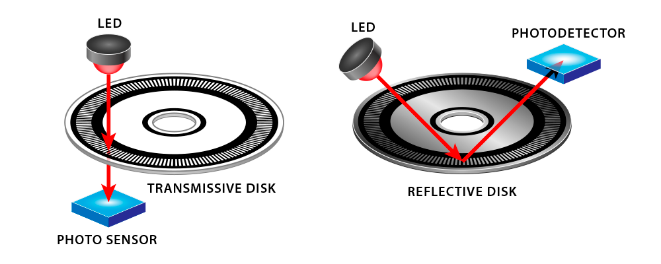
\includegraphics[width=0.7\linewidth]{figures/Chapter 4/Transimisive_vs_reflective.png}
    \caption{Transmissive vs. Reflective Encoder Configurations}
    \label{fig:encoder_types}
\end{figure}

\subsection{Encoder Data Acquisition Strategy}
\label{subsec:encoder_acquisition}

With 935 PPR encoders and target speeds up to 300 RPM, the signal frequency reaches approximately 4,675 Hz---a new pulse every 213 microseconds. Two architectural approaches were evaluated:

\subsubsection{Polling vs. Interrupt-Driven Architecture}

\paragraph{Polling (Rejected)}
In polling, the CPU continuously checks GPIO pin states in the main loop. However, the ESP32 handles Wi-Fi, micro-ROS communication, and PID calculations. If any task blocks the CPU for more than 200$\mu$s, pulses are missed, causing incorrect velocity readings and erratic behavior.

\paragraph{Interrupt Service Routines (Selected)}
We adopted an event-driven architecture using hardware interrupts. When a pin voltage transitions, the GPIO controller triggers the CPU to immediately execute an Interrupt Service Routine (ISR), increment the counter, and return to the main task. This guarantees atomic data capture with nanosecond-scale latency regardless of CPU load.

\paragraph{Critical Implementation: IRAM\_ATTR}
ESP32 program code typically resides in external Flash memory. If an interrupt fires while Flash is busy, the system crashes. The solution is the \texttt{IRAM\_ATTR} macro:

\begin{lstlisting}[language=C, caption={ISR with IRAM\_ATTR for Flash-Independent Execution}]
void IRAM_ATTR motor0_isr() {
    encoder_count[0]++;
}
\end{lstlisting}

This directive places the ISR code in internal SRAM, ensuring zero-latency access even during Flash operations.

\subsection{Quadrature Encoding Selection}
\label{subsec:quadrature_selection}

Quadrature encoders produce two channels (A and B) offset by 90°, enabling direction sensing. Three encoding types exist: X1, X2, and X4, differing in which edges are counted.

\subsubsection{X1 Encoding Selection Rationale}

We selected X1 encoding (counting only rising edges of Channel A) over X4 for three reasons:

\paragraph{1. Computational Efficiency}
At 300 RPM with three motors:
\begin{itemize}
    \item \textbf{X4 Mode:} $3740 \times 5 \times 3 = 56,100$ ISR calls/second
    \item \textbf{X1 Mode:} $935 \times 5 \times 3 = 14,025$ ISR calls/second
\end{itemize}

X1 reduces CPU overhead by 75\%, preserving cycles for Wi-Fi and micro-ROS communication.

\paragraph{2. Noise Immunity}
X4 is vulnerable to the ``dither problem''---when a motor stops on an encoder edge, vibration causes rapid signal toggling, accumulating phantom counts. X1 requires a full signal cycle to register a count, acting as a natural hysteresis filter.

\paragraph{3. Sufficient Resolution}
At 935 ticks/rev ($\approx 0.38°$/tick), even at low speeds (60 RPM) with a 50Hz control loop, the encoder registers $\approx$18 ticks per cycle---sufficient granularity for smooth PID control.

\subsection{Encoder Calibration}
\label{subsec:encoder_calibration}

Accurate PPR determination is critical for odometry. We used the ``Encoder Shaft'' method---tracking rotation directly at the encoder disc, bypassing gearbox backlash errors.

\paragraph{Procedure:}
\begin{enumerate}
    \item Remove the motor's rear cap to expose the encoder disc
    \item Attach a micro-marker to the rotating magnet
    \item Rotate exactly one revolution (360°) while recording tick count
    \item Repeat 20 times per motor and average results
\end{enumerate}

\paragraph{Result:} The calibration converged to \textbf{935 PPR}, which was hardcoded into the firmware.

\subsection{Velocity Estimation and Signal Processing}
\label{subsec:velocity_estimation}

Deriving velocity $\omega = \frac{d\theta}{dt}$ from discrete encoder ticks introduces quantization noise, particularly problematic for the PID derivative term.

\subsubsection{The Quantization Problem}

At 60 RPM with a 50Hz control loop, readings fluctuate between 18-19 ticks per cycle. This ``staircase'' signal creates high-frequency spikes in the derivative calculation, causing motor humming and instability.

\subsubsection{Solution: First-Order Low-Pass Filter}

We implemented an Exponential Moving Average (EMA) filter:

\begin{equation}
\hat{\omega}[k] = \alpha \cdot \omega_{raw}[k] + (1-\alpha) \cdot \hat{\omega}[k-1]
\label{eq:lowpass_filter}
\end{equation}

Where:
\begin{itemize}
    \item $\hat{\omega}[k]$ = filtered velocity estimate
    \item $\omega_{raw}[k]$ = raw velocity from encoder ticks
    \item $\alpha$ = smoothing factor (0 to 1)
\end{itemize}

\paragraph{Tuning:} Through step response analysis, we selected $\alpha = 0.1$. This provides sufficient noise rejection to stabilize the derivative term while introducing only $\approx$60ms phase lag---well within the stability margins of the robot's mechanical inertia.


\newpage
\section{Control Strategy and Controller Selection}
\label{sec:control_strategy}

To regulate the angular velocity of the omnidirectional wheels, a comparative analysis of three standard control architectures was conducted: Proportional-Integral-Derivative (PID), Linear Quadratic Regulator (LQR), and Model Predictive Control (MPC). The selection criteria focused on computational efficiency, model dependency, and suitability for the ESP32-S3 hardware constraints.

\subsection{Controller Selection Analysis}
\label{subsec:controller_selection}

Table~\ref{tab:controller_selection} presents a weighted decision matrix comparing the three controller architectures across four critical criteria.

\begin{table}[H]
    \centering
    \caption{Controller Selection Matrix}
    \label{tab:controller_selection}
    \begin{tabular}{|l|c|c|c|c|}
        \hline
        \textbf{Selection Criteria} & \textbf{Weight} & \textbf{MPC} & \textbf{LQR} & \textbf{PID} \\
        \hline
        Computational Cost & 30\% & 1 & 3 & 5 \\
        \hline
        Model Dependency & 30\% & 1 & 2 & 5 \\
        \hline
        Constraint Handling & 15\% & 4 & 2 & 2 \\
        \hline
        Application Suitability & 25\% & 1 & 2 & 5 \\
        \hline
        \textbf{Final Score} & --- & \textbf{1.45} & \textbf{2.30} & \textbf{4.55} \\
        \hline
    \end{tabular}
\end{table}

\subsubsection{Computational Cost}
\begin{itemize}
    \item \textbf{PID:} Extremely low. Requires only basic arithmetic (multiplication/addition) for three terms. Easily runs at $>$1kHz on ESP32.
    \item \textbf{LQR:} Low/Medium. Requires matrix multiplication of the state vector by the gain matrix $\mathbf{K}$. Efficient but requires full state feedback.
    \item \textbf{MPC:} Very high. Requires solving a Quadratic Programming (QP) optimization problem at every time step. Infeasible to run three parallel instances at 50Hz on an ESP32 while managing the Wi-Fi stack.
\end{itemize}

\subsubsection{Model Dependency}
\begin{itemize}
    \item \textbf{PID:} Model-free. Does not require a physics model of the motor (inductance, inertia, friction). Tunable via heuristics.
    \item \textbf{LQR:} High dependency. Requires an accurate state-space representation. If the physical motor parameters (friction coefficient, moment of inertia) change or are unknown, performance degrades significantly.
    \item \textbf{MPC:} Critical dependency. Relies entirely on the predictive model. Any mismatch between the model and reality leads to poor prediction and instability.
\end{itemize}

\subsubsection{Constraint Handling}
\begin{itemize}
    \item \textbf{PID:} Saturation (clamping) is added manually to handle voltage limits (Anti-Windup).
    \item \textbf{LQR:} None. Does not inherently handle actuator saturation.
    \item \textbf{MPC:} Native constraint handling capability, but this feature is unnecessary for simple speed regulation where clamping suffices.
\end{itemize}

\subsubsection{Application Suitability}
\begin{itemize}
    \item \textbf{PID:} Ideal for SISO (Single-Input Single-Output) systems where the objective is setpoint tracking (maintaining RPM).
    \item \textbf{LQR:} Best suited for MIMO (Multi-Input Multi-Output) regulation and stabilization (e.g., balancing an inverted pendulum) rather than simple reference tracking.
    \item \textbf{MPC:} Best suited for complex trajectory planning where future states must be optimized (e.g., autonomous driving pathing), not low-level actuator control.
\end{itemize}

\subsubsection{Selection Conclusion}
The \textbf{PID Controller} was selected because the motor system is treated as three independent SISO systems. The prohibitive computational cost of MPC and the high model-dependency of LQR were unjustified for a system where the physical parameters (friction, load) fluctuate dynamically during operation.

\subsection{Mathematical Derivation: Discrete PID Algorithm}
\label{subsec:discrete_pid}

The standard continuous-time PID equation is defined as:
\begin{equation}
    u(t) = K_p \cdot e(t) + K_i \int e(t) \, dt + K_d \cdot \frac{de(t)}{dt}
    \label{eq:pid_continuous}
\end{equation}

However, microcontrollers operate in discrete time steps. To implement this on the ESP32-S3, the equation was discretized using the Backward Euler Method with a sampling time $T_s = 20$ms (50Hz).

\subsubsection{Proportional Term}
\begin{equation}
    P[k] = K_p \cdot e[k]
    \label{eq:pid_p}
\end{equation}

\subsubsection{Integral Term (Accumulation)}
The integral is approximated as the sum of errors multiplied by the sampling time:
\begin{equation}
    I[k] = I[k-1] + K_i \cdot e[k] \cdot T_s
    \label{eq:pid_i}
\end{equation}

This recursive addition allows the controller to eliminate steady-state error ($e_{ss}$) by accumulating output until the error reaches zero.

\subsubsection{Derivative Term (Difference)}
The derivative is approximated as the slope between the current and previous error:
\begin{equation}
    D[k] = K_d \cdot \frac{e[k] - e[k-1]}{T_s}
    \label{eq:pid_d}
\end{equation}

\subsubsection{Final Control Law}
The total control signal (PWM Duty Cycle) sent to the motor driver is:
\begin{equation}
    u[k] = P[k] + I[k] + D[k]
    \label{eq:pid_control_law}
\end{equation}

\subsection{Stability Augmentation: Anti-Windup Strategy}
\label{subsec:anti_windup}

A critical limitation of the standard Integral term is \textit{windup}. When the actuator reaches its physical limit (e.g., Max PWM = 255) but the error persists (e.g., the robot is blocked by an obstacle), the Integral term continues to accumulate virtually to infinity. When the obstacle is removed, the controller remains saturated for a prolonged period, causing dangerous overshooting.

To mitigate this, a \textbf{Clamping Anti-Windup} mechanism was implemented:
\begin{enumerate}
    \item \textbf{Calculate Tentative Output:} Compute $u_{calc} = P + I + D$
    \item \textbf{Check Saturation:} If $|u_{calc}| > u_{max}$:
    \begin{itemize}
        \item Clamp the final output $u[k]$ to $u_{max}$
        \item Freeze the Integral: Stop adding to $I[k]$ to prevent it from growing beyond the physical capacity of the system
    \end{itemize}
\end{enumerate}

The specific C++ implementation of the clamping logic is provided in Appendix A (Motor.cpp).

\subsection{Tuning Methodology}
\label{subsec:pid_tuning}

A significant engineering challenge was the \textbf{Concurrent Development Phase}, where the low-level firmware was being developed simultaneously with the mechanical assembly. This prevented traditional model-based tuning because the mass and inertia of the robot were constantly changing. A hybrid tuning approach was adopted.

\subsubsection{Phase 1: Heuristic Tuning (Ziegler-Nichols Variant)}
Performed on a test bench with ``free spinning'' wheels:
\begin{enumerate}
    \item Set $K_i$ and $K_d$ to zero
    \item Increase $K_p$ until the motor velocity oscillates around the setpoint
    \item Set $K_p$ to $0.5 \times K_{oscillation}$ to ensure stability
    \item Introduce $K_i$ incrementally to remove steady-state error (the difference between Target RPM and Actual RPM)
\end{enumerate}

\subsubsection{Phase 2: Pole Placement using MATLAB PID Tuner}
Once the robot was fully assembled (loaded condition), the MATLAB System Identification Toolbox was utilized:
\begin{enumerate}
    \item \textbf{Step Response Test:} A step input (0 to 100 PWM) was injected and the open-loop velocity response curve was logged.
    \item \textbf{Transfer Function Estimation:} The motor-wheel system was approximated as a first-order plant with dead time:
    \begin{equation}
        G(s) = \frac{K}{\tau s + 1}
        \label{eq:transfer_function}
    \end{equation}
    \item \textbf{Optimization:} The MATLAB PID Tuner app was used to solve for optimal gains that provided a Rise Time $< 0.2$s and Overshoot $< 5\%$.
\end{enumerate}
\newpage
\section{The Micro-ROS Architecture}
\label{sec:microros}

This section explains the communication bridge between the MCU and the high-level computer (Jetson/Laptop).

\subsection{Overview: Bridging Real-Time Embedded Systems with DDS}
\label{subsec:microros_overview}

The integration of resource-constrained microcontrollers (MCUs) into the Robot Operating System (ROS 2) ecosystem presents a fundamental architectural challenge. Standard ROS 2 nodes communicate using the Data Distribution Service (DDS) protocol---specifically RTPS (Real-Time Publish-Subscribe). DDS is a heavy, peer-to-peer protocol requiring significant memory for discovery caches, serialization buffers, and history scaling, often exceeding 1MB of RAM---far beyond the capacity of typical MCUs.

To resolve this, \textbf{micro-ROS} was implemented, a specialized variant designed to extend the DDS ``Global Data Space'' onto the ESP32-S3. Unlike simple serial bridges (e.g., rosserial) which use custom, non-standard framing, micro-ROS creates first-class ROS 2 nodes on the microcontroller, allowing them to interact seamlessly with the high-level system using standard message definitions.

\subsection{The Client-Agent Architecture}
\label{subsec:client_agent}

The micro-ROS framework abandons the peer-to-peer model of standard DDS in favor of a \textbf{Client-Agent topology}. This asymmetrical architecture offloads the heavy lifting of discovery and routing to a more powerful host machine.

\subsubsection{The Micro-ROS Client (ESP32-S3)}
\begin{itemize}
    \item Runs a lightweight implementation of the ROS 2 stack (based on \texttt{rclc})
    \item Does not store the ROS graph or discovery database
    \item Serializes messages and sends them point-to-point to the Agent
\end{itemize}

\subsubsection{The Micro-ROS Agent (Jetson/Laptop)}
The Agent acts as a \textbf{Stateful Proxy} or ``Broker,'' running as a standard ROS 2 node on the host computer with the following responsibilities:
\begin{enumerate}
    \item \textbf{Translation:} Converts the lightweight Micro-XRCE-DDS messages from the MCU into standard DDS RTPS packets for the rest of the ROS 2 network
    \item \textbf{Discovery:} Handles the ROS 2 discovery traffic (Participant announcements) on behalf of the MCU
    \item \textbf{Entity Management:} Maintains the state of Publishers, Subscribers, and Services created by the MCU
\end{enumerate}

\begin{figure}[H]
    \centering
    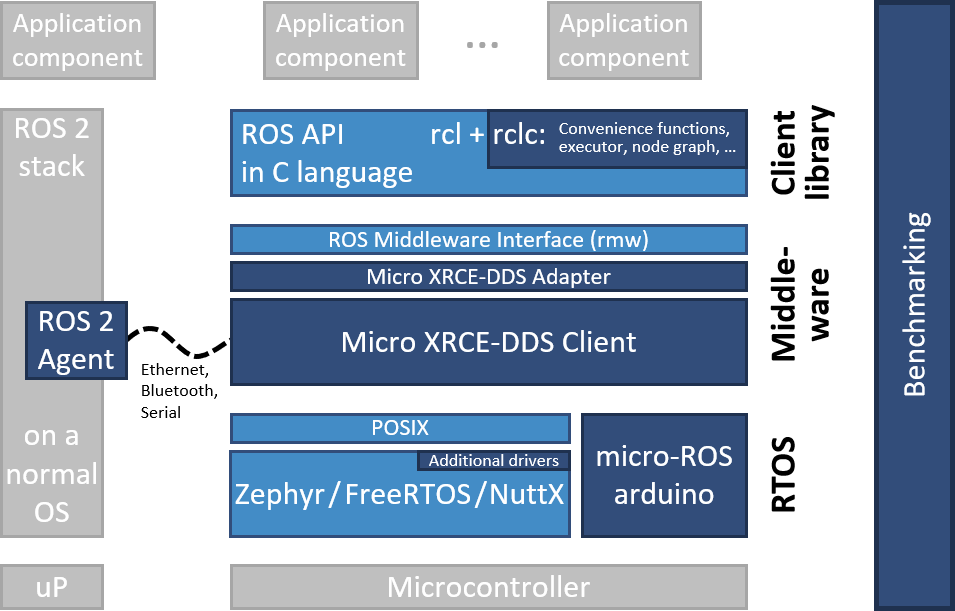
\includegraphics[width=0.85\linewidth]{figures/Chapter 4/Micro_ros_architecture.png}
    \caption{Micro-ROS Client-Agent Architecture}
    \label{fig:microros_architecture}
\end{figure}

\subsection{The Middleware: Micro-XRCE-DDS}
\label{subsec:xrce_dds}

At the heart of the communication layer lies \textbf{Micro-XRCE-DDS} (eXtremely Resource Constrained Environments---Data Distribution Service), an ISO standard protocol (OMG DDS-XRCE) optimized for embedded devices.

\subsubsection{Protocol Efficiency}
Unlike standard DDS, which creates dynamic connections for every topic, XRCE-DDS utilizes a stateless connection model for data transmission to minimize overhead:
\begin{itemize}
    \item \textbf{Serialization:} Uses CDR (Common Data Representation) with reduced header sizes compared to RTPS
    \item \textbf{Memory Footprint:} Designed to operate with $<$50KB of RAM, making it feasible to run alongside the Wi-Fi stack and motor control tasks on the ESP32-S3
\end{itemize}

\subsubsection{Transport Layer Agnosticism}
A critical engineering feature of Micro-XRCE-DDS is its separation from the physical transport layer. This allowed the construction of a dual-transport system:

\paragraph{UDP over Wi-Fi (UDPv4)}
\begin{itemize}
    \item \textbf{Selected for:} Development and Telemetry
    \item \textbf{Mechanism:} Uses IP addressing to stream data wirelessly, enabling ``Hardware-in-the-Loop'' style debugging where the robot moves freely while streaming live encoder data to the laptop
\end{itemize}

\paragraph{UART Serial}
\begin{itemize}
    \item \textbf{Selected for:} Deployment
    \item \textbf{Mechanism:} Uses a direct wired connection (Tx/Rx) to the Jetson, eliminating latency jitter and radio interference risks in industrial environments
    \item \textbf{Note:} The application logic remains identical; only the transport configuration struct is modified
\end{itemize}

\subsection{Deep Dive: The Micro-ROS Agent}
\label{subsec:agent_deep_dive}

The Agent is not merely a pass-through pipe; it is a complex server that manages the lifecycle of the embedded node.

\subsubsection{Connection Mechanics and Handshake}
Connecting to the Agent is a rigorous, multi-step handshake process handled by the \texttt{rmw\_microxrcedds} layer:

\paragraph{Session Initiation}
\begin{enumerate}
    \item The ESP32 sends a \texttt{CREATE\_SESSION} request containing a unique Session ID and Client Key
    \item The Agent checks if a session with that ID already exists; if not, it allocates memory structures to track the new client
    \item \textbf{Implementation Detail:} A static Agent IP (192.168.x.x) was hardcoded for Wi-Fi trials to bypass the complexity of UDP broadcast discovery, ensuring faster boot times ($<$2 seconds)
\end{enumerate}

\paragraph{Entity Creation (The ``Graph'' Build)}
Once the session is established, the MCU sends discrete requests to create entities:
\begin{itemize}
    \item \texttt{create\_participant}
    \item \texttt{create\_topic} (e.g., \texttt{/cmd\_vel})
    \item \texttt{create\_publisher} / \texttt{create\_subscriber}
\end{itemize}

The Agent executes these requests on the ROS 2 network. If the Agent crashes, these entities disappear from the ROS graph immediately, providing an inherent ``Liveliness'' check.

\subsubsection{Running the Agent}
For the implementation, a Dockerized version of the Agent was utilized to ensure environment consistency across different development machines (Ubuntu 22.04 / Linux Mint):
\begin{lstlisting}[language=bash, caption={Micro-ROS Agent Launch Command}]
ros2 run micro_ros_agent micro_ros_agent udp4 --port 8888
\end{lstlisting}

Port 8888 is the standard UDP listening port that the ESP32 targets in its transport configuration.

\subsection{Implementation Strategy: The rclc Executor}
\label{subsec:rclc_executor}

On the ESP32 side, the \texttt{rclc} (ROS Client Library for C) was utilized, which provides a C-API wrapper around the middleware. This is distinct from the C++ (\texttt{rclcpp}) or Python (\texttt{rclpy}) libraries used on the PC.

\subsubsection{Memory Management (Allocators)}
Dynamic memory allocation (\texttt{malloc}) is dangerous in embedded systems due to heap fragmentation. Micro-ROS requires a custom allocator---the FreeRTOS-compatible allocator was configured to reserve a static memory block for the ROS stack, ensuring that message generation never causes a ``Heap Overflow'' during runtime.

\subsubsection{The Executor Pattern}
Unlike the callback-based spin of standard ROS 2, \texttt{rclc} gives the developer granular control over execution:

\begin{lstlisting}[language=C, caption={rclc Executor Initialization (Simplified)}]
// Initialize executor with 2 handles
rclc_executor_init(&executor, &context, 2, &allocator);

// Add subscription and timer
rclc_executor_add_subscription(&executor, &sub_cmd_vel, &msg, &callback);
rclc_executor_add_timer(&executor, &timer_pub);
\end{lstlisting}

\paragraph{Determinism:} The Executor was configured to run in the main \texttt{loop()} with a short timeout. This polling-based execution (\texttt{rclc\_executor\_spin\_some}) allows deterministic interleaving of communication tasks with motor control tasks, preventing the Wi-Fi stack from starving the PID loop.

\subsection{Quality of Service (QoS) and Reliability}
\label{subsec:qos}

One of the most significant technical decisions in this architecture was the tuning of the Quality of Service (QoS) policies for Wi-Fi transport.

\subsubsection{The Problem: ``Reliable'' Overhead}
By default, ROS 2 uses a \textbf{Reliable} policy where the middleware guarantees delivery. If a packet is dropped (common in Wi-Fi), the sender halts and retries.

\textbf{Consequence:} On a mobile robot, a momentary Wi-Fi glitch would cause the \texttt{cmd\_vel} stream to pause. When the connection resumes, the robot might receive a burst of old, outdated velocity commands, causing dangerous, jerky behavior.

\subsubsection{The Solution: ``Best Effort'' (UDP-Style)}
The micro-ROS publishers and subscribers were explicitly configured to use \texttt{rmw\_qos\_profile\_sensor\_data} (Best Effort):
\begin{itemize}
    \item \textbf{Behavior:} The system attempts to send the packet once; if lost, it is discarded
    \item \textbf{Rationale:} For real-time velocity commands, if a packet arrives late, it is useless. It is better to skip a frame and wait for the fresh command than to delay the entire system trying to recover old data
\end{itemize}

This configuration proved vital for the smoothness of the ``Square Path'' demonstration.

\subsection{Section Summary}
\label{subsec:microros_summary}

This architecture effectively creates a distributed computing system where the ``Brain'' (Jetson) and ``Muscle'' (ESP32) are loosely coupled by a standardized protocol (DDS-XRCE), yet tightly integrated in terms of data flow. The use of the Agent as an intermediary allows the heavy ROS 2 stack to remain on the host, while the Client remains lightweight enough to run alongside critical 50Hz motor control loops.

\begin{figure}[H]
    \centering
    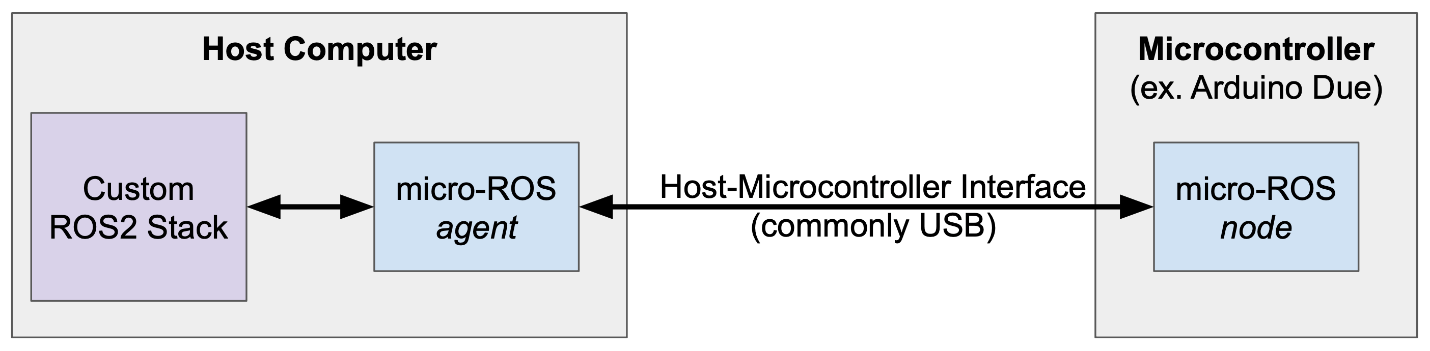
\includegraphics[width=0.7\linewidth]{figures/Chapter 4/Section_summary.png}
    \caption{Micro-ROS Communication Summary}
    \label{fig:microros_summary}
\end{figure}

\newpage
\section{Evolutionary Architecture: The Three-Phase Iteration}
\label{sec:evolutionary_architecture}

The development of the low-level control subsystem followed an iterative process of architectural exploration, driven by competing constraints of hard real-time performance, soft real-time communication, and development velocity.

\subsection{Trial 1: RTOS-Native Approach}
\label{subsec:trial1}

\subsubsection{Hypothesis}
Running micro-ROS as a prioritized task directly within the FreeRTOS kernel would offer the highest determinism by eliminating Arduino framework overhead.

\subsubsection{Implementation}
The \texttt{micro\_ros\_setup} component was integrated into ESP-IDF with a preemptive scheduling architecture:
\begin{itemize}
    \item \texttt{Task\_Transport} (Priority 2): Wi-Fi and UDP handling
    \item \texttt{Task\_MicroROS} (Priority 3): rclc executor processing
    \item \texttt{Task\_MotorControl} (Priority 5): Hard real-time PID at 50Hz
\end{itemize}

\subsubsection{Failure Mode}
\begin{itemize}
    \item \textbf{Stack Overflows:} The XRCE-DDS serialization layer is stack-intensive; tuning stack depth was precarious
    \item \textbf{Build Complexity:} Cross-compiling for the specific FreeRTOS kernel required complex CMake modifications with $>$3 minute build times
    \item \textbf{Conclusion:} Maintenance overhead outweighed marginal scheduling gains
\end{itemize}

\subsection{Trial 2: Bare-Metal ESP-IDF Optimization}
\label{subsec:trial2}

\subsubsection{Hypothesis}
Using ESP-IDF's native hardware peripherals without ROS abstraction would maximize hardware efficiency with near-zero CPU load.

\subsubsection{Implementation}
\begin{itemize}
    \item \textbf{PCNT Peripheral:} Hardware pulse counter for encoder reading with zero CPU overhead
    \item \textbf{LEDC Peripheral:} Hardware PWM generation with jitter-free duty cycles
\end{itemize}

\subsubsection{Failure Mode}
\begin{itemize}
    \item \textbf{Software Gap:} ESP-IDF's C-based framework required writing PID, kinematics, and vector math libraries from scratch
    \item \textbf{Brittleness:} Custom low-level drivers made pin configuration changes require register-level rewrites
    \item \textbf{Conclusion:} The ESP32-S3's dual-core 240MHz processor was powerful enough without extreme PCNT optimization; development time cost was unjustified
\end{itemize}

\subsection{Trial 3: Hybrid Architecture (Final Solution)}
\label{subsec:trial3}

The final architecture leverages Arduino Core for rapid hardware abstraction while retaining micro-ROS for robust communication.

\subsubsection{Dual-Core Asymmetric Processing}
\begin{itemize}
    \item \textbf{Core 0 (Protocol):} Wi-Fi stack and micro-ROS Agent communication
    \item \textbf{Core 1 (Application):} PID calculations and Encoder ISRs
\end{itemize}

This isolation ensures Wi-Fi packet bursts never interrupt encoder tick reading.

\subsubsection{IRAM-Resident ISRs}
The \texttt{IRAM\_ATTR} macro places ISRs in high-speed internal SRAM, eliminating cache-miss crashes and reducing interrupt latency to nanoseconds.

\subsubsection{Atomic Data Access}
Race conditions are prevented using critical sections:
\begin{lstlisting}[language=C, caption={Atomic Encoder Read}]
noInterrupts();  // Critical section start
long safe_counts = encoder_count;
interrupts();    // Critical section end
\end{lstlisting}

\subsubsection{Validation Results}
\begin{itemize}
    \item \textbf{Stability:} $>$30 minutes continuous operation without crashes
    \item \textbf{Responsiveness:} End-to-end latency $<$15ms (keypress to motor)
    \item \textbf{Safety:} 500ms software watchdog integration for failsafe operation
\end{itemize}

\section{Summary}
\label{sec:electrical_summary}

This chapter has presented the complete electrical architecture and embedded software design of the AUSRA robot platform. The key contributions are summarized as follows:

\begin{enumerate}
    \item \textbf{System Architecture:} A hierarchical control topology was established with the NVIDIA Jetson Orin Nano as the high-level ``Brain'' and the ESP32-S3 as the low-level ``Spine,'' enabling decoupled AI processing from real-time motor control.
    
    \item \textbf{Component Selection:} Through weighted decision matrices:
    \begin{itemize}
        \item The \textbf{ESP32-S3} was selected for its micro-ROS compatibility, dual-core architecture, and cost efficiency (Score: 8.80/10)
        \item The \textbf{Cytron MDD3A} provides MOSFET efficiency with 50\% current headroom and integrated protection (Score: 63)
        \item The \textbf{Total P20S 20V battery} offers integrated BMS, charge-in-place capability, and 72-minute runtime (Score: 9.6/10)
    \end{itemize}
    
    \item \textbf{Power Management:} A three-state hardware switch (Charge/Idle/Run) ensures operational safety, while dual-stage buck conversion isolates logic from motor noise.
    
    \item \textbf{Low-Level Firmware:} Quadrature encoders (935 PPR) with X1 encoding provide velocity feedback through IRAM-resident ISRs, processed by an EMA filter ($\alpha = 0.1$) for noise rejection.
    
    \item \textbf{Control Strategy:} A discrete PID controller was selected over LQR and MPC for its model-free operation and computational efficiency, with clamping anti-windup for stability. Tuning employed Ziegler-Nichols heuristics followed by MATLAB PID Tuner optimization.
    
    \item \textbf{Micro-ROS Integration:} The Client-Agent architecture bridges the ESP32 to the ROS 2 ecosystem via Micro-XRCE-DDS, with Best Effort QoS ensuring smooth real-time velocity command delivery over Wi-Fi.
    
    \item \textbf{Software Evolution:} Three architectural trials led to the final hybrid solution (Arduino + micro-ROS), achieving dual-core task separation, $<$15ms end-to-end latency, and $>$30 minutes continuous stability.
\end{enumerate}

These design choices collectively enable the AUSRA platform to achieve reliable autonomous operation while maintaining the modularity, safety, and real-time performance required for swarm robotics research.

% ============================================================================
% Chapter 5: High-Level Configuration & Autonomous Stack
% ============================================================================

\chapter{Autonomous Navigation Stack: Architecture and Simulation}
\label{chap:autonomous}

This chapter presents the hardware selection, software architecture, and autonomous navigation stack of the AUSRA system, including the high-level computing platform, localization, path planning, motion control, and swarm communication.

\section{High-Level Computing Architecture}
\label{sec:highlevel_computing}

\subsection{System Requirements}
\label{subsec:system_requirements}

The AUSRA platform requires a robust high-level computing subsystem capable of handling decentralized autonomy in dynamic, unstructured environments. The system must satisfy requirements across four critical domains:

\begin{figure}[H]
    \centering
    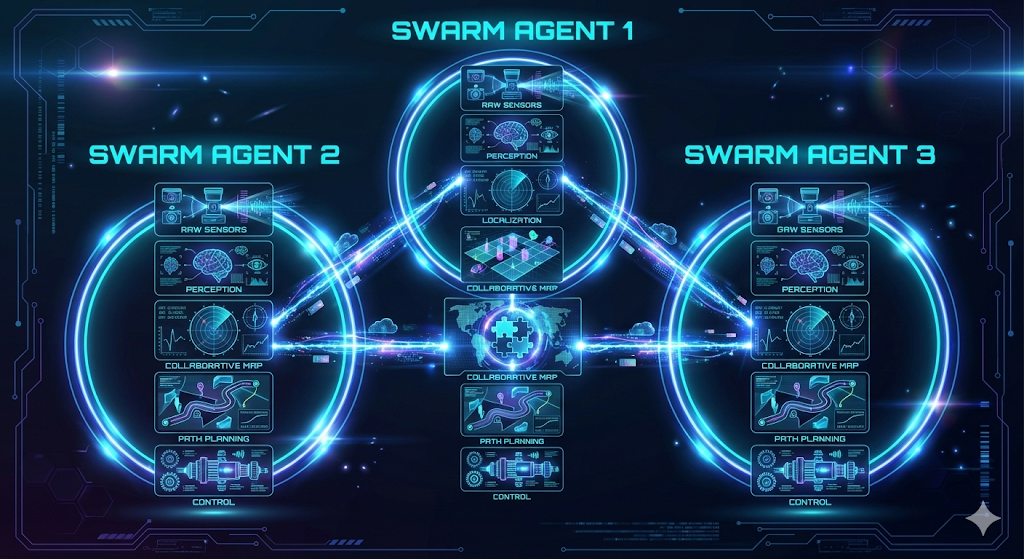
\includegraphics[width=0.85\linewidth]{figures/Chapter 5/High_level_swarm.png}
    \caption{High-Level Swarm Architecture Overview}
    \label{fig:high_level_swarm}
\end{figure}

\subsubsection{Perception Requirements}
The perception module must process dense sensor data in real-time for reliable obstacle avoidance and object detection:
\begin{itemize}
    \item High-resolution LiDAR scans for local costmap construction
    \item Depth camera feeds for dynamic entity detection
    \item Sensor fusion algorithms (Extended Kalman Filter) without latency at 0.2 m/s operating velocity
    \item Neural network inference for on-the-fly object classification
\end{itemize}

\subsubsection{Communication Requirements}
The architecture must support decentralized swarm coordination:
\begin{itemize}
    \item Inter-robot data exchange (telemetry, map fragments, task allocation)
    \item Full-featured OS for network stack and DDS middleware (ROS 2)
    \item Complex message serialization without blocking navigation threads
\end{itemize}

\subsubsection{Navigation and Control Requirements}
\begin{itemize}
    \item Global path planning (A*/Dijkstra) through known map data
    \item Local trajectory adjustment for collision avoidance
    \item Omnidirectional velocity computation ($v_x$, $v_y$, $\omega$) at high frequency
    \item Minimal jitter to prevent drift and localization errors
\end{itemize}

\begin{figure}[H]
    \centering
    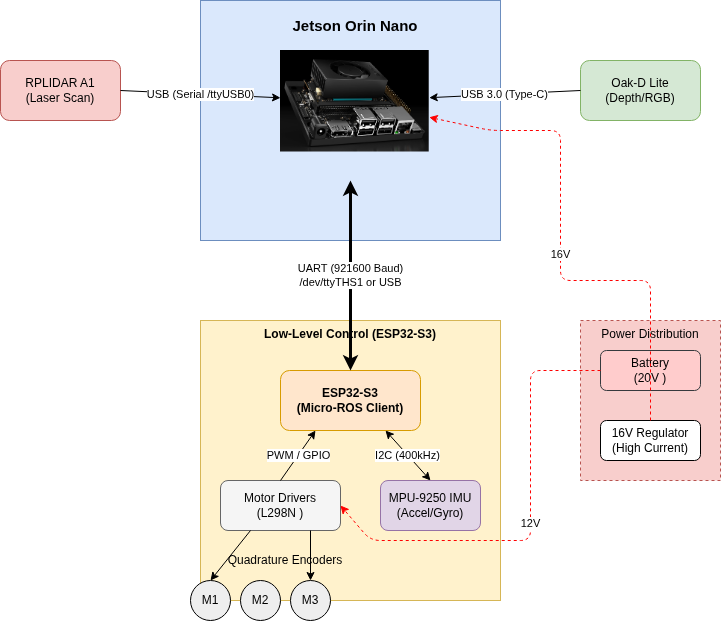
\includegraphics[width=0.8\linewidth]{figures/Chapter 5/Hardware_architecture.png}
    \caption{Hardware Architecture Block Diagram}
    \label{fig:hardware_architecture}
\end{figure}

\subsection{Computing Platform Analysis}
\label{subsec:computing_analysis}

Two leading embedded computing platforms were evaluated: Raspberry Pi 5 and NVIDIA Jetson Orin Nano.

\subsubsection{Raspberry Pi 5}

\begin{figure}[H]
    \centering
    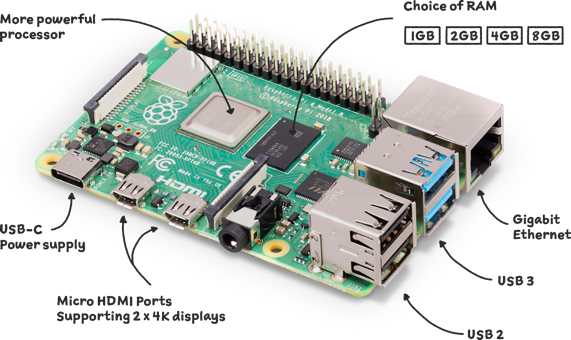
\includegraphics[width=0.5\linewidth]{figures/Chapter 5/Raspbery_pi_5.png}
    \caption{Raspberry Pi 5}
    \label{fig:raspberry_pi}
\end{figure}

The Raspberry Pi 5 represents the standard for general-purpose embedded computing:

\paragraph{Strengths}
\begin{itemize}
    \item Quad-core ARM Cortex-A76 processor
    \item Versatile I/O: dual HDMI, Gigabit Ethernet, USB 3.0, 40-pin GPIO
    \item Massive community support and mature Debian-based OS
    \item Simplified ROS 2 installation
\end{itemize}

\paragraph{Limitations}
\begin{itemize}
    \item No hardware acceleration for AI/ML workloads
    \item CPU-bound processing for point clouds and neural networks
    \item VideoCore GPU designed for multimedia, not parallel computing
    \item Thermal throttling under sustained heavy loads causes latency spikes
\end{itemize}

\subsubsection{NVIDIA Jetson Orin Nano}

\begin{figure}[H]
    \centering
    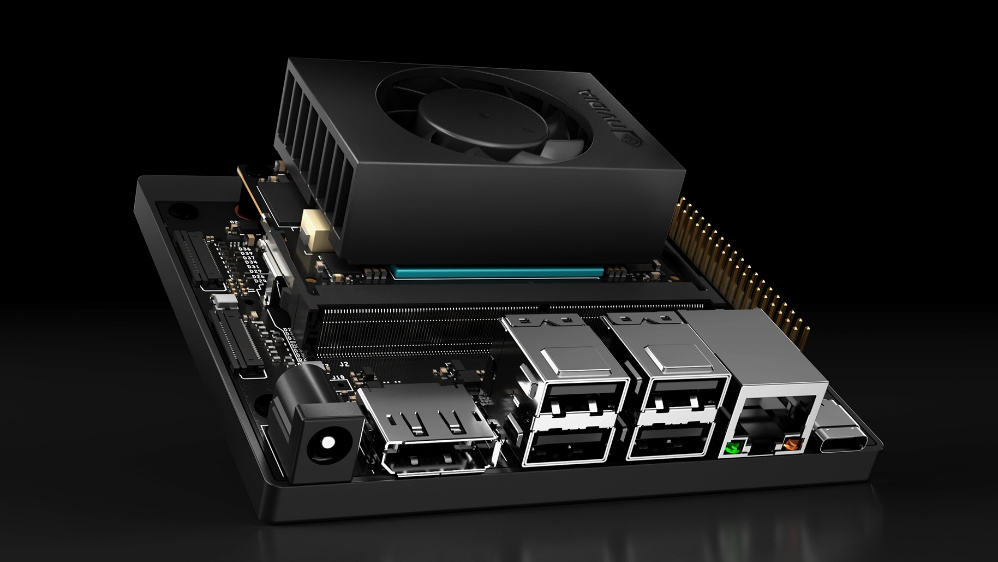
\includegraphics[width=0.5\linewidth]{figures/Chapter 5/Jetson_orin_nano.jpg}
    \caption{NVIDIA Jetson Orin Nano Development Kit}
    \label{fig:jetson_orin}
\end{figure}

The Jetson Orin Nano is engineered specifically for edge AI and autonomous robotics:

\paragraph{Strengths}
\begin{itemize}
    \item NVIDIA Ampere GPU: 1024 CUDA cores, 32 Tensor Cores
    \item Up to 40 TOPS AI performance
    \item 6-core ARM Cortex-A78AE processor
    \item M.2 Key M for NVMe SSD support
    \item JetPack SDK with CUDA-X, TensorRT, and ISAAC ROS libraries
    \item Development kit includes heatsink and fan assembly
\end{itemize}

\paragraph{Limitations}
\begin{itemize}
    \item Higher cost and complexity
    \item Requires carrier board and robust power supply
    \item Increased power consumption during GPU operations
    \item Larger thermal solution adds to physical footprint
\end{itemize}

\subsection{Platform Selection}
\label{subsec:platform_selection}

\begin{figure}[H]
    \centering
    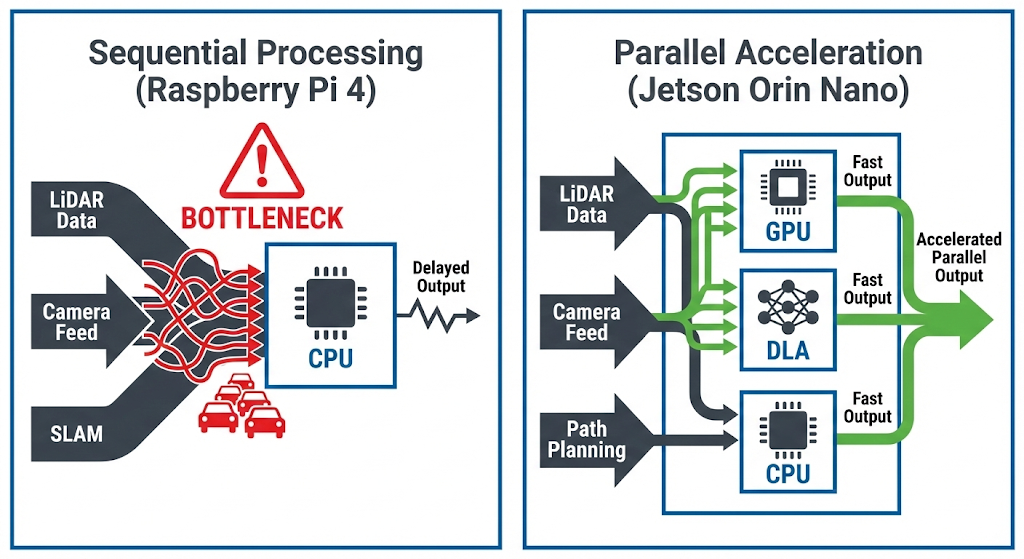
\includegraphics[width=0.75\linewidth]{figures/Chapter 5/pi5_vs_jetson_comparison.png}
    \caption{Raspberry Pi 5 vs. Jetson Orin Nano Comparison}
    \label{fig:pi_vs_jetson}
\end{figure}

The \textbf{NVIDIA Jetson Orin Nano} was selected as the high-level controller for the following reasons \cite{nvidia2023jetson}:

\begin{enumerate}
    \item \textbf{SLAM and Object Detection:} The Raspberry Pi's sequential CPU processing is insufficient for simultaneous localization, mapping, and real-time inference.
    
    \item \textbf{Perception Pipeline:} GPU-accelerated capabilities ensure latency-free processing of dense LiDAR data and neural network models.
    
    \item \textbf{Development Environment:} Ample memory bandwidth supports the full ROS 2 desktop environment and debugging tools directly on the robot.
    
    \item \textbf{Future-Proofing:} The hardware architecture ensures computing capacity does not become the limiting factor as swarm intelligence complexity increases.
\end{enumerate}

\subsection{Depth Camera Selection}
\label{subsec:depth_camera}

Visual perception enables environmental understanding beyond proprioceptive sensors, supporting obstacle detection, visual odometry, robot tracking for swarm coordination, and object recognition.

\subsubsection{Camera Technology Comparison}

\begin{figure}[H]
    \centering
    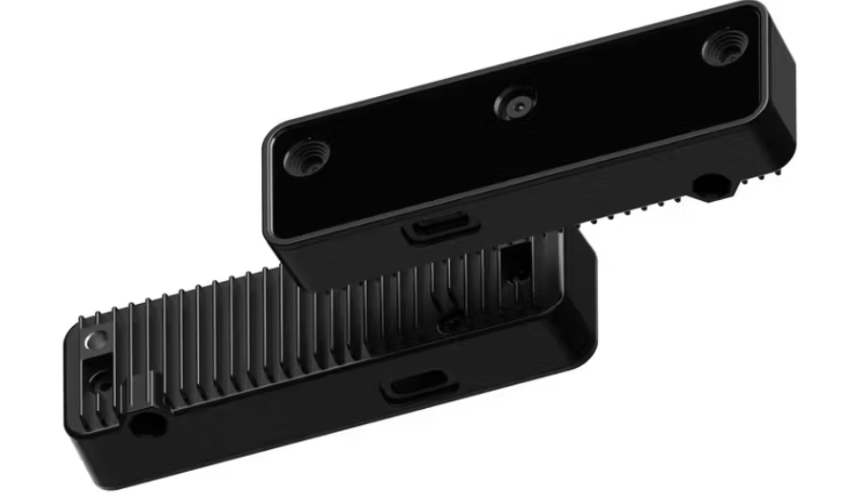
\includegraphics[width=0.6\linewidth]{figures/Chapter 5/cam_1.png}
    \caption{Luxonis OAK-D Lite Depth Camera}
    \label{fig:oakd_lite}
\end{figure}

Four camera technologies were evaluated: monocular RGB, stereo depth, Time-of-Flight (ToF), and structured light.

\begin{table}[H]
\centering
\caption{Camera Configuration Selection Matrix}
\label{tab:camera_config}
\begin{tabular}{|l|c|c|c|c|}
\hline
\textbf{Criteria} & \textbf{Weight} & \textbf{RGB} & \textbf{Stereo Depth} & \textbf{ToF} \\
\hline
Depth Accuracy & 5 & 5 & 20 & 25 \\
\hline
Depth Range & 4 & 4 & 20 & 12 \\
\hline
Computational Efficiency & 4 & 20 & 12 & 20 \\
\hline
Cost & 4 & 20 & 16 & 8 \\
\hline
Environmental Robustness & 3 & 12 & 12 & 9 \\
\hline
Size \& Weight & 2 & 10 & 8 & 8 \\
\hline
\textbf{Final Score} & & \textbf{71} & \textbf{88} & \textbf{82} \\
\hline
\end{tabular}
\end{table}

\subsubsection{Depth Camera Model Comparison}

Three depth camera models were evaluated for the stereo depth configuration:

\begin{figure}[H]
    \centering
    \begin{subfigure}[b]{0.3\textwidth}
        \centering
        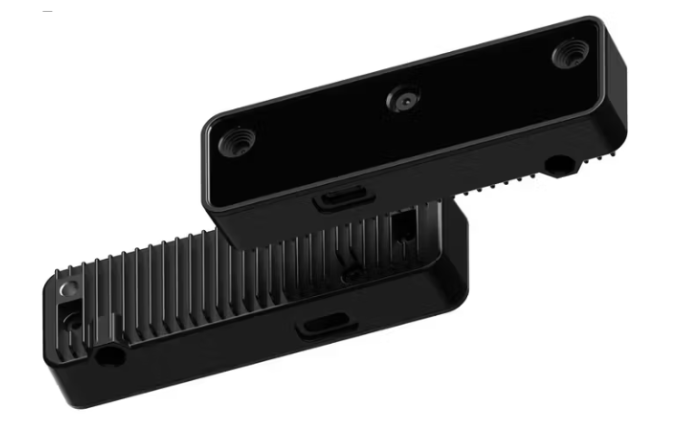
\includegraphics[width=\linewidth]{figures/Chapter 5/cam_4.png}
        \caption{OAK-D Lite}
        \label{fig:oakd_compare}
    \end{subfigure}
    \hfill
    \begin{subfigure}[b]{0.3\textwidth}
        \centering
        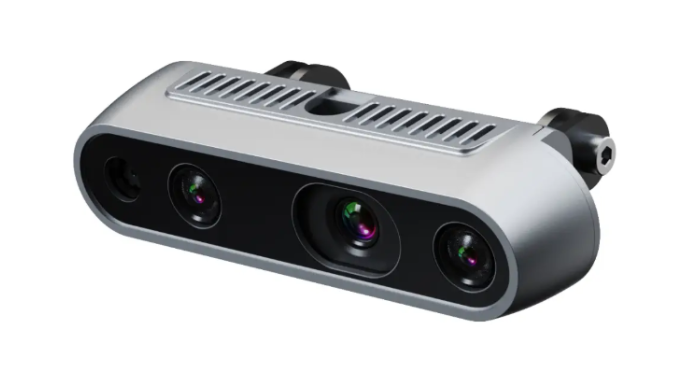
\includegraphics[width=\linewidth]{figures/Chapter 5/cam_5.png}
        \caption{Intel RealSense D435i}
        \label{fig:realsense_compare}
    \end{subfigure}
    \hfill
    \begin{subfigure}[b]{0.3\textwidth}
        \centering
        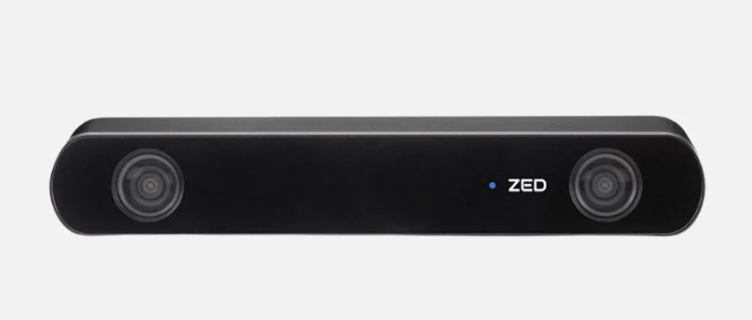
\includegraphics[width=\linewidth]{figures/Chapter 5/cam_6.png}
        \caption{ZED 2i}
        \label{fig:zed_compare}
    \end{subfigure}
    \caption{Depth Camera Candidates}
    \label{fig:depth_camera_candidates}
\end{figure}

\begin{table}[H]
\centering
\caption{Depth Camera Selection Matrix}
\label{tab:depth_camera_selection}
\begin{tabular}{|l|c|c|c|c|}
\hline
\textbf{Criteria} & \textbf{Weight} & \textbf{OAK-D Lite} & \textbf{RealSense D435i} & \textbf{ZED 2i} \\
\hline
Depth Performance & 5 & 20 & 20 & 25 \\
\hline
Onboard AI Processing & 4 & 20 & 4 & 12 \\
\hline
Cost Effectiveness & 4 & 20 & 12 & 8 \\
\hline
Size \& Weight & 3 & 15 & 12 & 9 \\
\hline
Software Ecosystem & 4 & 16 & 20 & 16 \\
\hline
Power Consumption & 3 & 15 & 12 & 9 \\
\hline
Multi-Robot Compatibility & 3 & 15 & 12 & 9 \\
\hline
\textbf{Final Score} & & \textbf{121} & \textbf{92} & \textbf{88} \\
\hline
\end{tabular}
\end{table}

\subsubsection{Final Selection: Luxonis OAK-D Lite}

The \textbf{OAK-D Lite} was selected based on \cite{luxonis2023oakd}:
\begin{enumerate}
    \item \textbf{Onboard AI Processing:} The Intel Myriad X VPU performs depth calculation and neural network inference locally, reducing latency and offloading computation from the Jetson.
    \item \textbf{Cost Advantage:} At approximately half the price of competitors, enables scaling to larger swarms within budget constraints.
    \item \textbf{Adequate Depth Performance:} 2--5 cm accuracy at 1 meter meets navigation requirements with appropriate safety margins.
    \item \textbf{Compact Form Factor:} 96.3 mm × 28.5 mm × 17.2 mm at 62 grams simplifies mechanical integration.
    \item \textbf{ROS 2 Integration:} The \texttt{depthai-ros} package provides excellent support with active development.
\end{enumerate}

\subsubsection{Hardware Specifications}

\begin{itemize}
    \item \textbf{Stereo Cameras:} Dual 1MP (1280×800) global shutter monochrome, 7.5 cm baseline
    \item \textbf{RGB Camera:} 4K (4056×3040) with autofocus
    \item \textbf{Depth Range:} 0.2--20 m (effective 0.5--10 m for indoor operation)
    \item \textbf{Field of View:} 71.9° × 56.6° (stereo), 68.8° × 55.5° (RGB)
    \item \textbf{Depth FPS:} Up to 60 fps at lower resolutions
    \item \textbf{Power:} 2.5W typical via USB 3.1 Type-C
    \item \textbf{AI Performance:} Myriad X VPU supports TensorFlow, PyTorch, OpenVINO models
\end{itemize}

\begin{figure}[H]
    \centering
    \begin{subfigure}[b]{0.45\textwidth}
        \centering
        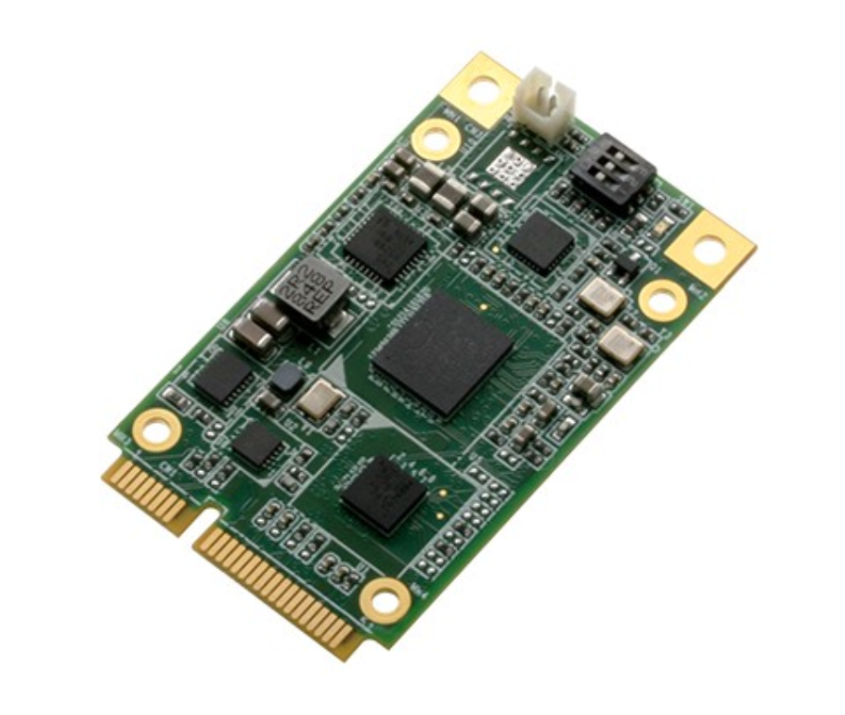
\includegraphics[width=\linewidth]{figures/Chapter 5/cam_2.png}
        \caption{OAK-D Lite System Architecture}
        \label{fig:oakd_architecture}
    \end{subfigure}
    \hfill
    \begin{subfigure}[b]{0.45\textwidth}
        \centering
        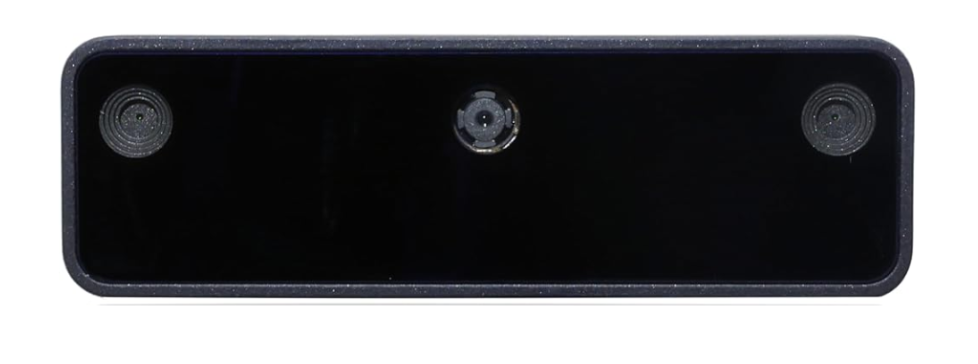
\includegraphics[width=\linewidth]{figures/Chapter 5/cam_3.png}
        \caption{Stereo Camera Configuration}
        \label{fig:stereo_config}
    \end{subfigure}
    \caption{OAK-D Lite Hardware Overview}
    \label{fig:oakd_hardware}
\end{figure}

\subsubsection{Application Scenarios}

\paragraph{Obstacle Detection and Collision Avoidance}
The depth image provides dense 3D point clouds for local occupancy maps, enabling detection of obstacles at varying heights---including overhanging objects and low barriers---that 2D LiDAR cannot capture.

\paragraph{Visual Odometry}
Feature tracking between frames provides independent velocity estimates, validating wheel encoder data during slip conditions when encoders report false movement.

\paragraph{Robot Detection and Swarm Coordination}
Neural network-based detection identifies teammate robots for formation control and collision avoidance, with depth providing direct 3D position relative to the detecting robot.

\paragraph{Semantic Scene Understanding}
Pixel-level classification (floor, wall, furniture, objects) supports task planning, while object recognition enables manipulation tasks for warehouse automation or search and rescue operations.

\begin{figure}[H]
    \centering
    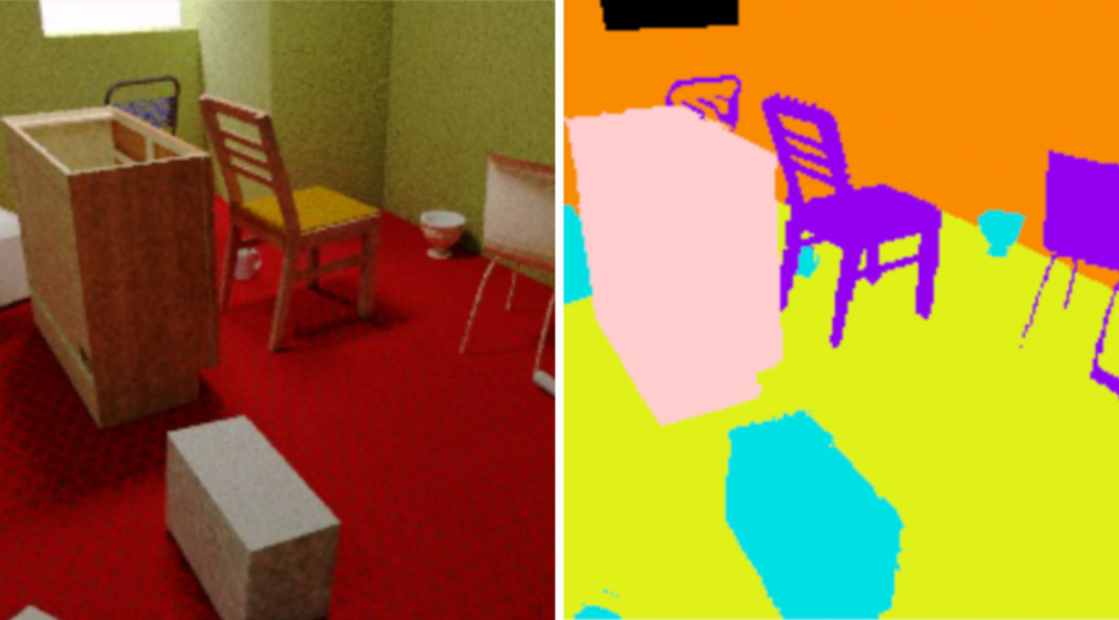
\includegraphics[width=0.7\linewidth]{figures/Chapter 5/cam_7.png}
    \caption{Semantic Segmentation Example}
    \label{fig:semantic_segmentation}
\end{figure}

\subsubsection{Mechanical Integration}

A custom 3D-printed PLA+ mounting bracket positions the camera at an elevated location maximizing forward and lateral field of view while maintaining structural rigidity. The mount resists vibration during robot operation and maintains stereo pair alignment for accurate depth calculation.

\begin{figure}[H]
    \centering
    \begin{subfigure}[b]{0.45\textwidth}
        \centering
        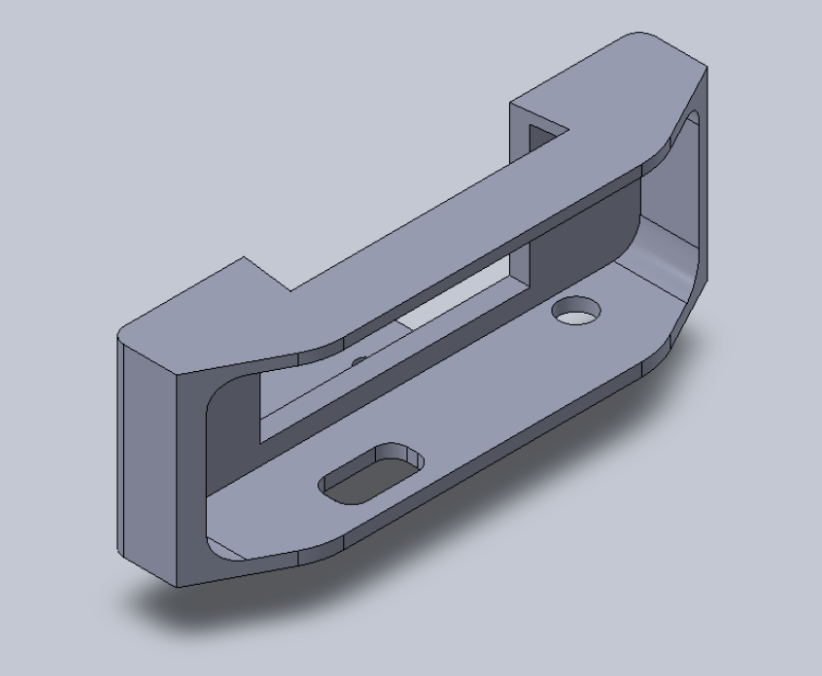
\includegraphics[width=\linewidth]{figures/Chapter 5/cam_8.png}
        \caption{Camera Mount Design}
        \label{fig:cam_mount_design}
    \end{subfigure}
    \hfill
    \begin{subfigure}[b]{0.45\textwidth}
        \centering
        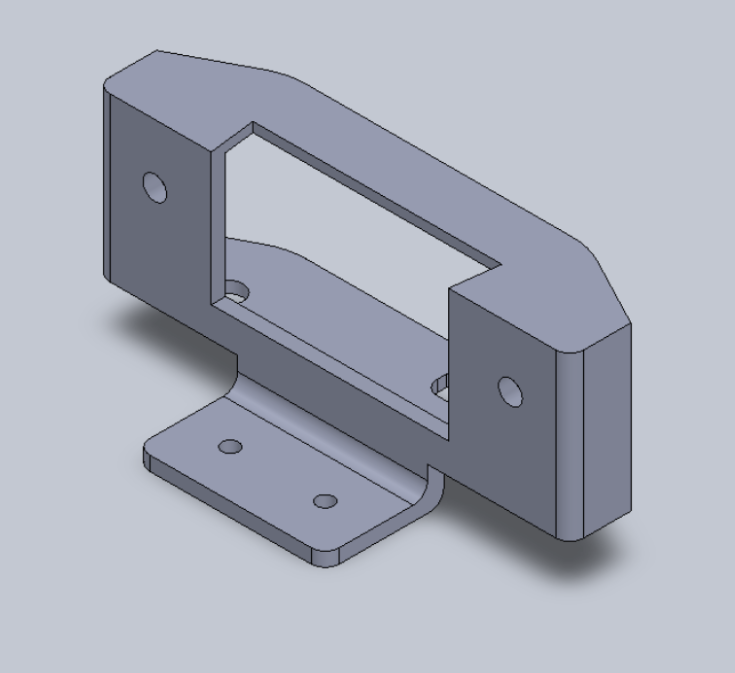
\includegraphics[width=\linewidth]{figures/Chapter 5/cam_9.png}
        \caption{Installed Camera Mount}
        \label{fig:cam_mount_installed}
    \end{subfigure}
    \caption{OAK-D Lite Mechanical Mounting}
    \label{fig:camera_mounting}
\end{figure}

\subsection{Inertial Measurement Unit Selection}
\label{subsec:imu_selection}

The IMU provides high-frequency measurements (100 Hz) of orientation, angular velocity, and linear acceleration---critical for navigation when other sensors are unavailable or compromised. It operates independently of environmental conditions, making it valuable during rapid rotations, dusty conditions, or areas with poor visual features.

\begin{figure}[H]
    \centering
    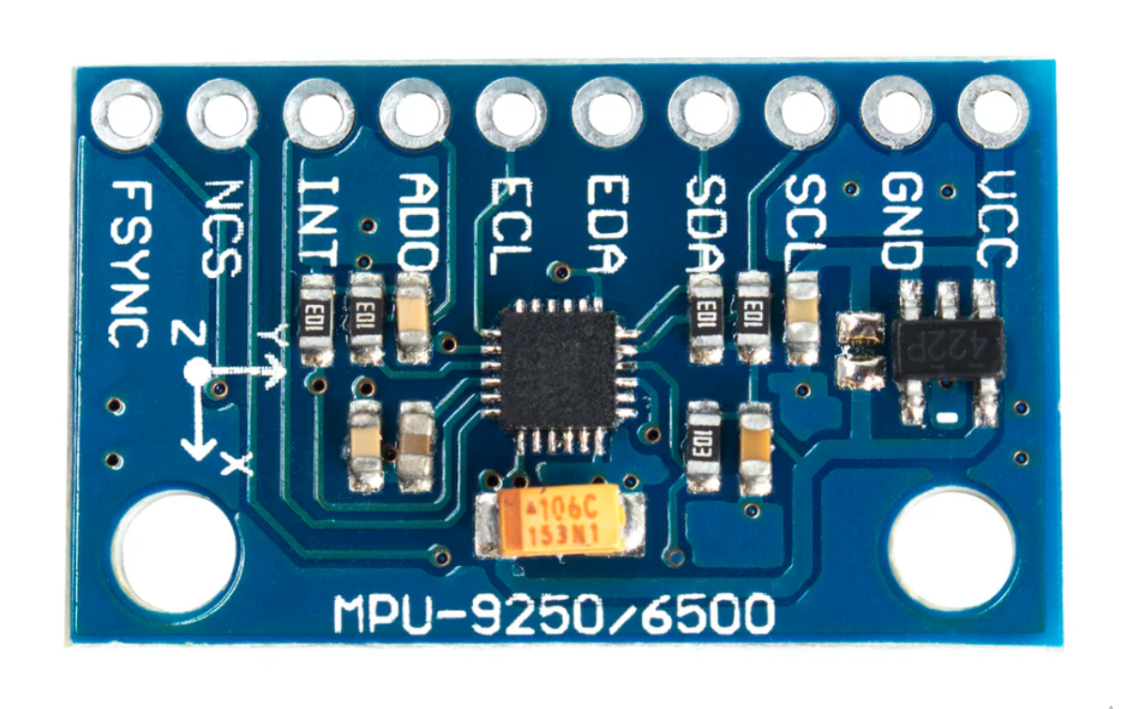
\includegraphics[width=0.5\linewidth]{figures/Chapter 5/IMU_image.png}
    \caption{MPU-9250 9-Axis IMU Module}
    \label{fig:imu_module}
\end{figure}

\subsubsection{IMU Configuration Comparison}

Three IMU configurations were evaluated: 6-axis (gyroscope + accelerometer), 9-axis (with magnetometer), and sensor fusion IMUs (with onboard processing).

\begin{table}[H]
\centering
\caption{IMU Configuration Selection Matrix}
\label{tab:imu_config}
\begin{tabular}{|l|c|c|c|c|}
\hline
\textbf{Criteria} & \textbf{Weight} & \textbf{6-Axis} & \textbf{9-Axis} & \textbf{Fusion IMU} \\
\hline
Accuracy \& Performance & 5 & 20 & 20 & 25 \\
\hline
Cost & 4 & 20 & 16 & 8 \\
\hline
Software Ecosystem & 4 & 16 & 20 & 16 \\
\hline
Size \& Weight & 3 & 15 & 15 & 9 \\
\hline
Power Consumption & 3 & 15 & 12 & 9 \\
\hline
Magnetometer Benefit & 2 & 2 & 10 & 10 \\
\hline
\textbf{Final Score} & & \textbf{88} & \textbf{93} & \textbf{67} \\
\hline
\end{tabular}
\end{table}

\subsubsection{IMU Model Comparison}

Three 9-axis IMU models were evaluated:

\begin{table}[H]
\centering
\caption{IMU Model Selection Matrix}
\label{tab:imu_model}
\begin{tabular}{|l|c|c|c|c|}
\hline
\textbf{Criteria} & \textbf{Weight} & \textbf{MPU-9250} & \textbf{BNO055} & \textbf{ICM-20948} \\
\hline
Sensor Performance & 5 & 20 & 25 & 25 \\
\hline
Cost-Effectiveness & 4 & 20 & 8 & 12 \\
\hline
Size \& Weight & 3 & 12 & 9 & 12 \\
\hline
Software Ecosystem & 4 & 20 & 16 & 12 \\
\hline
Power Consumption & 3 & 12 & 12 & 12 \\
\hline
Availability & 3 & 15 & 6 & 3 \\
\hline
\textbf{Final Score} & & \textbf{99} & \textbf{76} & \textbf{76} \\
\hline
\end{tabular}
\end{table}

\subsubsection{Final Selection: MPU-9250}

The \textbf{MPU-9250} was selected based on:
\begin{enumerate}
    \item \textbf{Software Ecosystem:} Extensive Arduino libraries, ROS drivers, and calibration tools with strong community support.
    \item \textbf{Cost Advantage:} At \$15--20 per unit (vs. \$35--45 for BNO055), enables 10-robot swarms for the cost of 4--5 premium-IMU robots.
    \item \textbf{Adequate Performance:} Gyroscope noise density 0.01°/s/$\sqrt{\text{Hz}}$, accelerometer noise density 300 $\mu$g/$\sqrt{\text{Hz}}$---sufficient for mobile robot navigation with EKF fusion.
    \item \textbf{I2C Compatibility:} 3.3V operation compatible with both ESP32-S3 (prototyping) and Jetson Orin Nano (production).
\end{enumerate}

\subsubsection{Hardware Specifications}

\begin{itemize}
    \item \textbf{Gyroscope:} 3-axis, $\pm$2000°/s range, 16-bit ADC
    \item \textbf{Accelerometer:} 3-axis, $\pm$16g range, 16-bit ADC
    \item \textbf{Magnetometer:} 3-axis, $\pm$4800 $\mu$T range
    \item \textbf{Interface:} I2C at 400 kHz (Fast Mode)
    \item \textbf{Update Rate:} 100 Hz configured
    \item \textbf{Power:} 3.3V, low consumption
\end{itemize}

\subsubsection{Hardware Implementation}

\begin{figure}[H]
    \centering
    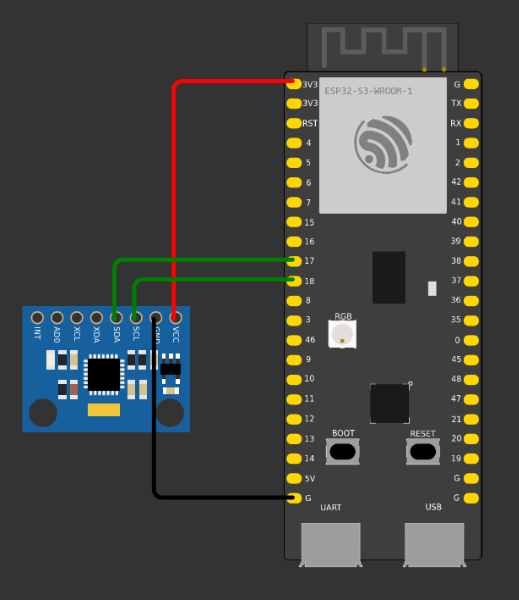
\includegraphics[width=0.6\linewidth]{figures/Chapter 5/IMU_circuit_schematic.png}
    \caption{IMU I2C Connection Schematic}
    \label{fig:imu_schematic}
\end{figure}

A custom interface PCB was developed for mechanical stability and maintenance:
\begin{itemize}
    \item \textbf{Header-Based Interface:} 5-pin configuration (VCC, GND, SCL, SDA, EDA) for quick sensor swapping
    \item \textbf{Terminal Blocks:} Screw-type connectors prevent vibration-induced disconnections
    \item \textbf{Rigid Mounting:} M3 bolts secure PCB to chassis, maintaining alignment with \texttt{base\_link} frame
\end{itemize}

\begin{figure}[H]
    \centering
    \begin{subfigure}[b]{0.3\textwidth}
        \centering
        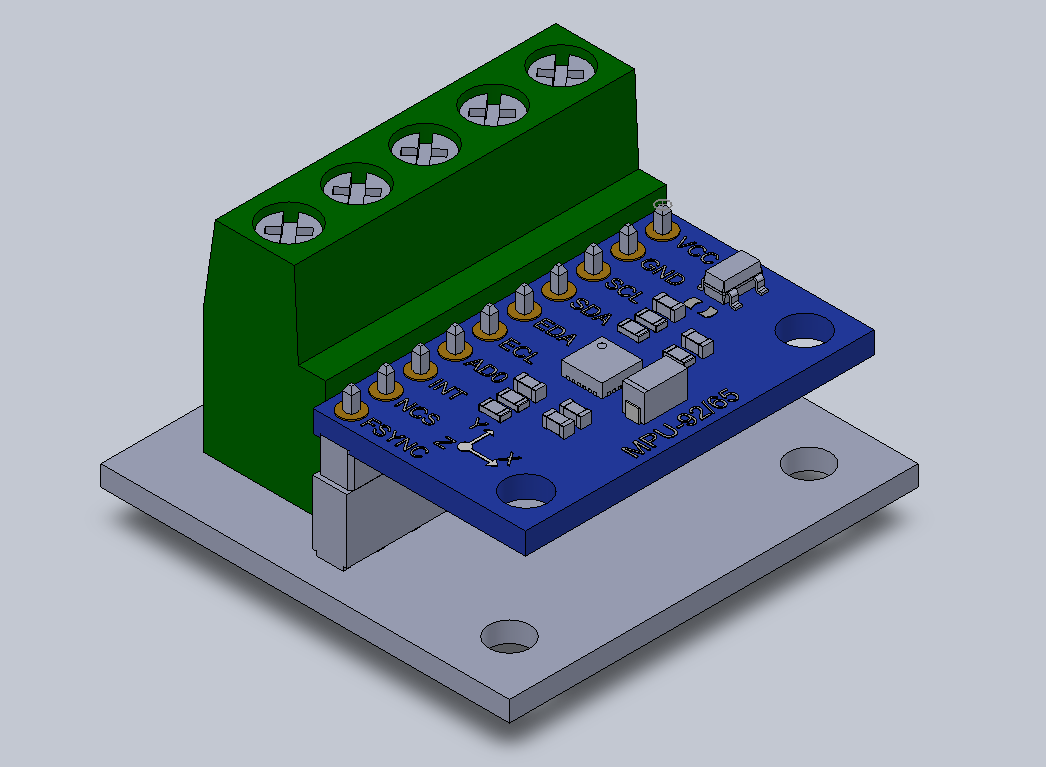
\includegraphics[width=\linewidth]{figures/Chapter 5/IMU_pcb_1.png}
        \caption{PCB Design}
        \label{fig:imu_pcb1}
    \end{subfigure}
    \hfill
    \begin{subfigure}[b]{0.3\textwidth}
        \centering
        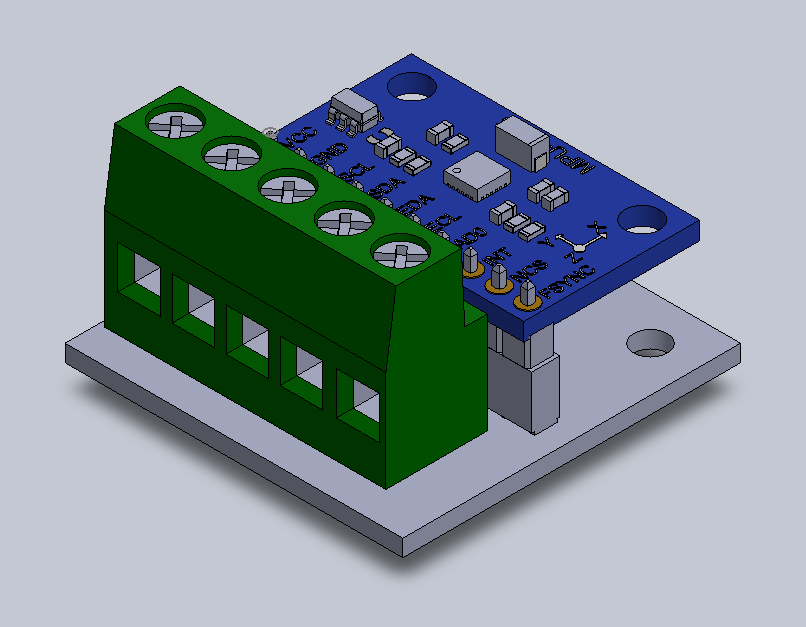
\includegraphics[width=\linewidth]{figures/Chapter 5/IMU_pcb_2.png}
        \caption{Assembled PCB}
        \label{fig:imu_pcb2}
    \end{subfigure}
    \hfill
    \begin{subfigure}[b]{0.3\textwidth}
        \centering
        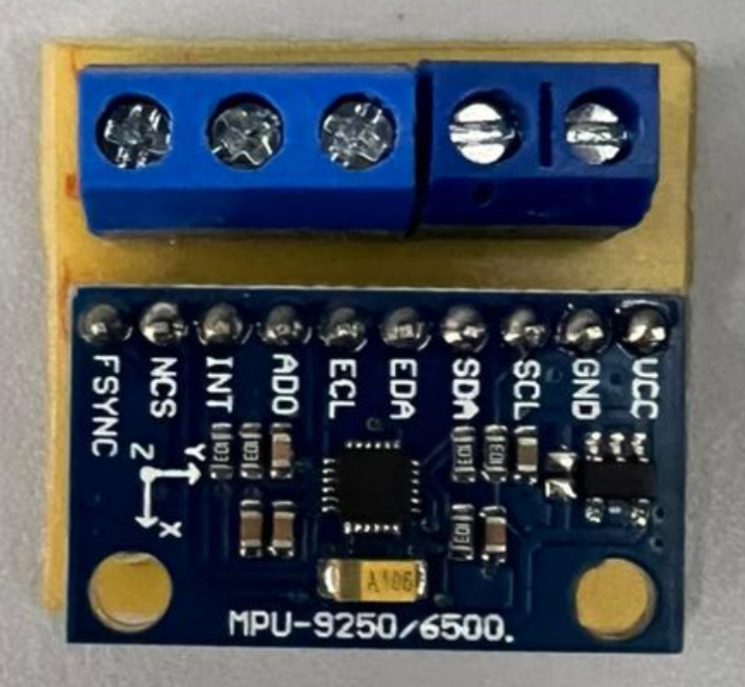
\includegraphics[width=\linewidth]{figures/Chapter 5/IMU_pcb_3.png}
        \caption{Mounted Assembly}
        \label{fig:imu_pcb3}
    \end{subfigure}
    \caption{IMU Custom Interface PCB}
    \label{fig:imu_pcb}
\end{figure}

\subsubsection{Calibration Procedures}

\paragraph{Accelerometer and Gyroscope Calibration}
At startup, 500 samples are collected with the sensor stationary on a horizontal surface. Outliers ($>$2$\sigma$ from mean) are rejected before averaging to determine bias values.

\paragraph{Magnetometer Calibration}
Requires rotation through full range of orientations to characterize hard-iron offsets (constant fields) and soft-iron distortions. A standardized figure-eight procedure for 20 seconds around each axis ensures consistent calibration.

\subsection{LiDAR Selection}
\label{subsec:lidar_selection}

The primary exteroceptive sensor provides geometric perception of the environment through laser scanning. LiDAR measures distance using Time-of-Flight (ToF) principles: a laser pulse is emitted at time $t_0$, reflects off obstacles, and returns at time $t_1$. The distance is calculated as:
\begin{equation}
d = \frac{c \cdot \Delta t}{2}
\label{eq:lidar_distance}
\end{equation}
where $c$ is the speed of light and $\Delta t = t_1 - t_0$.

The output in polar coordinates $(r, \theta)$ is converted to Cartesian coordinates:
\begin{equation}
x_{robot} = r \cdot \cos(\theta), \quad y_{robot} = r \cdot \sin(\theta)
\label{eq:lidar_cartesian}
\end{equation}

\subsubsection{2D vs. 3D LiDAR Comparison}

\begin{table}[H]
\centering
\caption{LiDAR Type Selection Matrix}
\label{tab:lidar_type}
\begin{tabular}{|l|c|c|c|c|c|}
\hline
\textbf{Criteria} & \textbf{Weight} & \multicolumn{2}{c|}{\textbf{2D LiDAR}} & \multicolumn{2}{c|}{\textbf{3D LiDAR}} \\
\cline{3-6}
 & & Rating & Score & Rating & Score \\
\hline
Swarm Scalability (Cost) & 5 & 5 & 25 & 0 & 0 \\
\hline
Field of View (FOV) & 5 & 5 & 25 & 5 & 25 \\
\hline
Computational Efficiency & 4 & 5 & 20 & 1 & 4 \\
\hline
Range \& Accuracy & 3 & 3 & 9 & 5 & 15 \\
\hline
ROS 2 Integration & 3 & 5 & 15 & 5 & 15 \\
\hline
\textbf{Final Score} & & & \textbf{94} & & \textbf{59} \\
\hline
\end{tabular}
\end{table}

\subsubsection{Final Selection: RPLIDAR A1}

\begin{figure}[H]
    \centering
    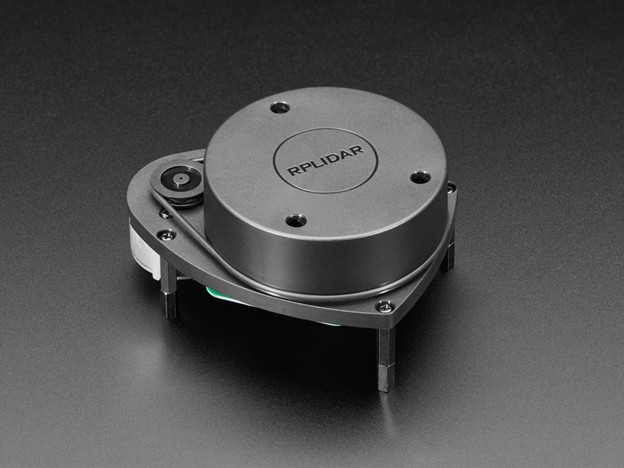
\includegraphics[width=0.4\linewidth]{figures/Chapter 5/rplidar.jpg}
    \caption{RPLIDAR A1 360-Degree 2D Laser Scanner}
    \label{fig:rplidar}
\end{figure}

The \textbf{RPLIDAR A1} was selected based on \cite{slamtec2023rplidar}:
\begin{itemize}
    \item \textbf{360° FOV:} Complete environmental awareness in a single scan
    \item \textbf{Cost-Effective:} Enables swarm scalability at \$99 per unit
    \item \textbf{Sufficient Range:} 12m range adequate for indoor navigation
    \item \textbf{Low Computational Load:} 2D point clouds enable real-time SLAM on embedded platforms
    \item \textbf{Mature ROS 2 Support:} Official SLAMTEC driver package
\end{itemize}

\paragraph{Hardware Specifications}
\begin{itemize}
    \item \textbf{Range:} 0.15--12 m
    \item \textbf{Angular Resolution:} $<$1° (5.5 Hz scan rate)
    \item \textbf{Scan Rate:} 5.5--10 Hz configurable
    \item \textbf{Interface:} USB (Serial/UART)
    \item \textbf{Power:} 5V, 500mA typical
\end{itemize}

\subsubsection{ROS 2 Integration}

\paragraph{Hardware Driver}
The official SLAMTEC ROS 2 driver provides hardware abstraction:
\begin{itemize}
    \item Communicates via USB serial
    \item Controls motor speed (PWM)
    \item Parses raw byte stream into \texttt{sensor\_msgs/LaserScan}
\end{itemize}

\paragraph{Simulation Driver}
In Gazebo, a ray sensor plugin simulates the LiDAR physics, outputting identical \texttt{LaserScan} messages for algorithm development.

\begin{figure}[H]
    \centering
    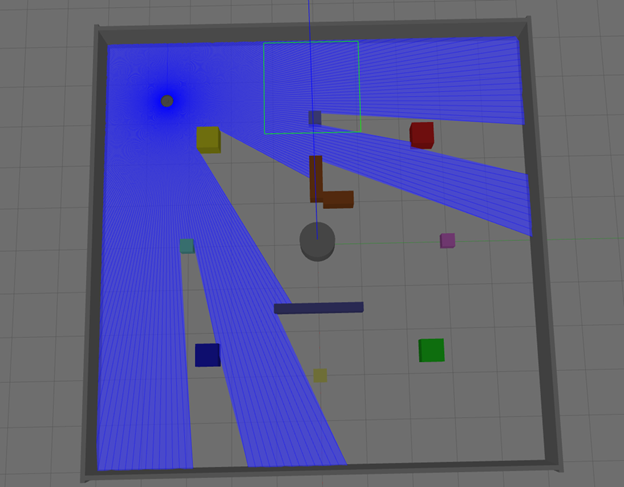
\includegraphics[width=0.7\linewidth]{figures/Chapter 5/lidar_rays_gazebo.png}
    \caption{LiDAR Simulation in Gazebo}
    \label{fig:lidar_gazebo}
\end{figure}

\paragraph{Data Output}
The standardized \texttt{sensor\_msgs/LaserScan} message contains:
\begin{itemize}
    \item \textbf{Header:} Timestamp and \texttt{frame\_id} for TF synchronization
    \item \textbf{Angle Increment:} Angular resolution between beams
    \item \textbf{Ranges Array:} Distance measurements to obstacles
\end{itemize}

\begin{figure}[H]
    \centering
    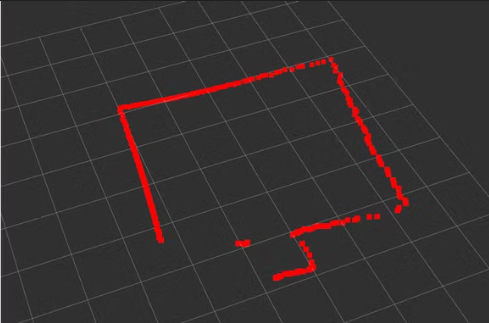
\includegraphics[width=0.7\linewidth]{figures/Chapter 5/lidar_laser_rviz.png}
    \caption{LiDAR Data Visualization in RViz2}
    \label{fig:lidar_rviz}
\end{figure}
\newpage
\section{System Architecture}
\label{sec:system_architecture}

\subsection{Software Stack Overview}
The AUSRA software stack utilizes a containerized approach to ensure portability and reproducibility. The architecture is built upon the Robot Operating System (ROS) framework \cite{quigley2009ros}, specifically ROS 2 Humble, which provides standardized interfaces for sensor integration, inter-process communication, and navigation.

\begin{figure}[H]
    \centering
    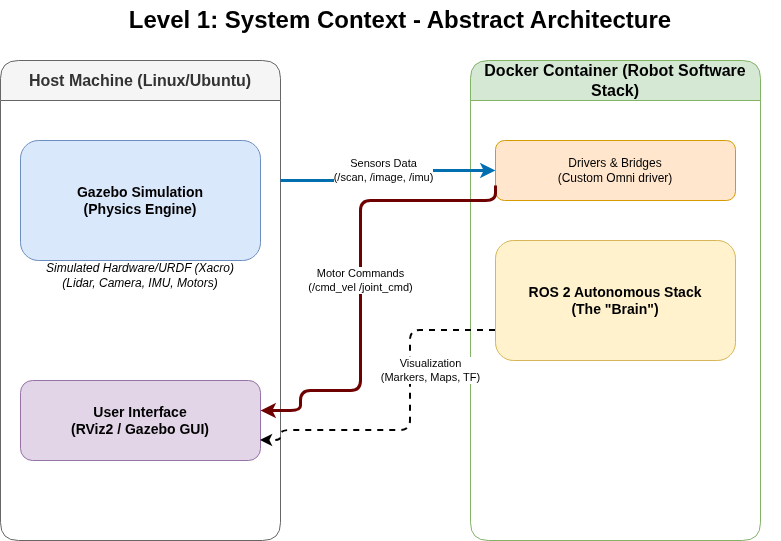
\includegraphics[width=0.9\linewidth]{figures/Chapter 5/Abstract_Architecture.png}
    \caption{Level 1: System Context - Abstract Architecture}
    \label{fig:abstract_arch}
\end{figure}

As illustrated in Figure \ref{fig:abstract_arch}, the architecture separates the simulation host from the robot software:
\begin{itemize}
    \item \textbf{Host Machine:} Runs the Gazebo Physics Engine and RViz2
    \item \textbf{Docker Container:} Encapsulates the complete ``Robot Brain'' (Drivers, SLAM, Nav2, Exploration)
\end{itemize}

\subsection{Key Software Components}
\begin{itemize}
    \item \textbf{Perception:} LiDAR and Depth Camera processing
    \item \textbf{Localization:} AMCL and SLAM Toolbox
    \item \textbf{Planning:} Global (A*) and local (DWB) path planners
    \item \textbf{Exploration:} Frontier-based autonomous mapping
    \item \textbf{Control:} Omnidirectional kinematics
\end{itemize}

\subsection{Low-Level Interface (micro-ROS)}

The system handles real-time hardware control using micro-ROS running on an ESP32-S3 microcontroller. This bridge connects the high-level ROS 2 stack (on the Jetson Orin Nano) with low-level actuators and sensors.

\begin{itemize}
    \item \textbf{Transport:} Communication via UART (Serial) at 921600 baud to minimize latency
    \item \textbf{Architecture:}
    \begin{itemize}
        \item \textbf{Client (ESP32-S3):} Runs the micro-ROS Client, implementing real-time PID loops for motor velocity control and reading raw IMU/Encoder data
        \item \textbf{Agent (Jetson Host):} Runs the \texttt{micro\_ros\_agent}, acting as a DDS proxy, making the embedded device's topics visible to the ROS 2 network
    \end{itemize}
    \item \textbf{Entities:} The ESP32 exposes:
    \begin{itemize}
        \item Subscribers: \texttt{/cmd\_vel} (Twist) for target velocities
        \item Publishers: \texttt{/odom} (Odometry) and \texttt{/imu/raw} (Sensor data)
    \end{itemize}
\end{itemize}

\subsection{Deployment on Jetson Orin Nano (Docker)}

The entire software stack is containerized for reliable deployment on the NVIDIA Jetson Orin Nano:

\begin{itemize}
    \item \textbf{Containerization:} A custom Docker image encapsulates ROS 2 Humble \cite{ros2design2020}, Nav2 \cite{nav2docs, macenski2020marathon2}, SLAM Toolbox, and all dependencies, preventing ``dependency hell'' and ensuring consistent library versions
    \item \textbf{Network Configuration:} Containers use \texttt{network\_mode: host}, allowing DDS middleware to access host network interfaces for multicast discovery---critical for swarm communication
    \item \textbf{Hardware Acceleration:} Docker configured with NVIDIA Container Runtime (\texttt{--runtime nvidia}), granting ROS nodes GPU access for accelerated perception
\end{itemize}

\subsection{Core ROS 2 Node Overview}

The autonomous stack comprises several interconnected ROS 2 nodes, each responsible for a specific function in the perception-planning-control pipeline:

\begin{table}[H]
\centering
\caption{Core ROS 2 Nodes and Their Functions}
\label{tab:ros_nodes}
\begin{tabular}{|l|p{4.5cm}|p{5cm}|}
\hline
\textbf{Node Name} & \textbf{Function} & \textbf{Key Topics} \\
\hline
\texttt{rplidar\_node} & LiDAR data acquisition & Pub: \texttt{/scan} \\
\texttt{imu\_serial\_node} & IMU data acquisition & Pub: \texttt{/imu/data\_raw}, \texttt{/imu/mag} \\
\texttt{ekf\_node} & EKF sensor fusion & Sub: \texttt{/imu/data\_raw}, \texttt{/wheel/odom} \newline Pub: \texttt{/odometry/filtered}, \texttt{/tf} \\
\texttt{slam\_toolbox} & SLAM and mapping & Sub: \texttt{/scan}, \texttt{/tf} \newline Pub: \texttt{/map}, \texttt{/tf} \\
\texttt{bt\_navigator} & Behavior tree navigation & Sub: \texttt{/goal\_pose} \newline Pub: Navigation actions \\
\texttt{planner\_server} & Global path planning (A*) & Pub: \texttt{/plan} \\
\texttt{controller\_server} & Local trajectory control (DWB) & Pub: \texttt{/cmd\_vel} \\
\texttt{omni\_driver} & Inverse kinematics \& odometry & Sub: \texttt{/cmd\_vel} \newline Pub: \texttt{/wheel/odom}, \texttt{/wheel\_cmd} \\
\texttt{micro\_ros\_agent} & ESP32 communication bridge & DDS $\leftrightarrow$ Serial \\
\hline
\end{tabular}
\end{table}

The data flow follows the standard ROS 2 navigation architecture: sensors feed into localization and mapping nodes, which provide the environmental context for the Nav2 planning and control servers, ultimately producing velocity commands executed by the omnidirectional driver.

\section{Simulation Environment}
\label{sec:simulation}

The AUSRA system is validated in a high-fidelity simulation environment using Gazebo Classic. The simulation runs on the host machine and communicates with the autonomous stack (in Docker) via standard ROS 2 interfaces.

\subsection{Testing Scenarios}

Several distinct environments stress-test different aspects of the system:

\begin{itemize}
    \item \textbf{Basic Verification (Rooms 1 \& 2):} Simple, enclosed environments for unit testing navigation, mapping quality, and obstacle avoidance
    \item \textbf{Disaster Response (Office Earthquake):} Complex, unstructured environment representing a collapsed office building with debris, narrow passageways, and clutter \cite{marder2010office}---designed for Frontier Exploration and constrained navigation testing
    \item \textbf{Coordination (Multi-Robot Room):} Large, open environment for swarm testing with multiple agents to verify Collaborative SLAM and decentralized avoidance
\end{itemize}

An example of the semantic construction of these worlds (SDF format) is provided in Appendix \ref{app:sim_code}.

\begin{figure}[H]
    \centering
    \begin{subfigure}[b]{0.48\textwidth}
        \centering
        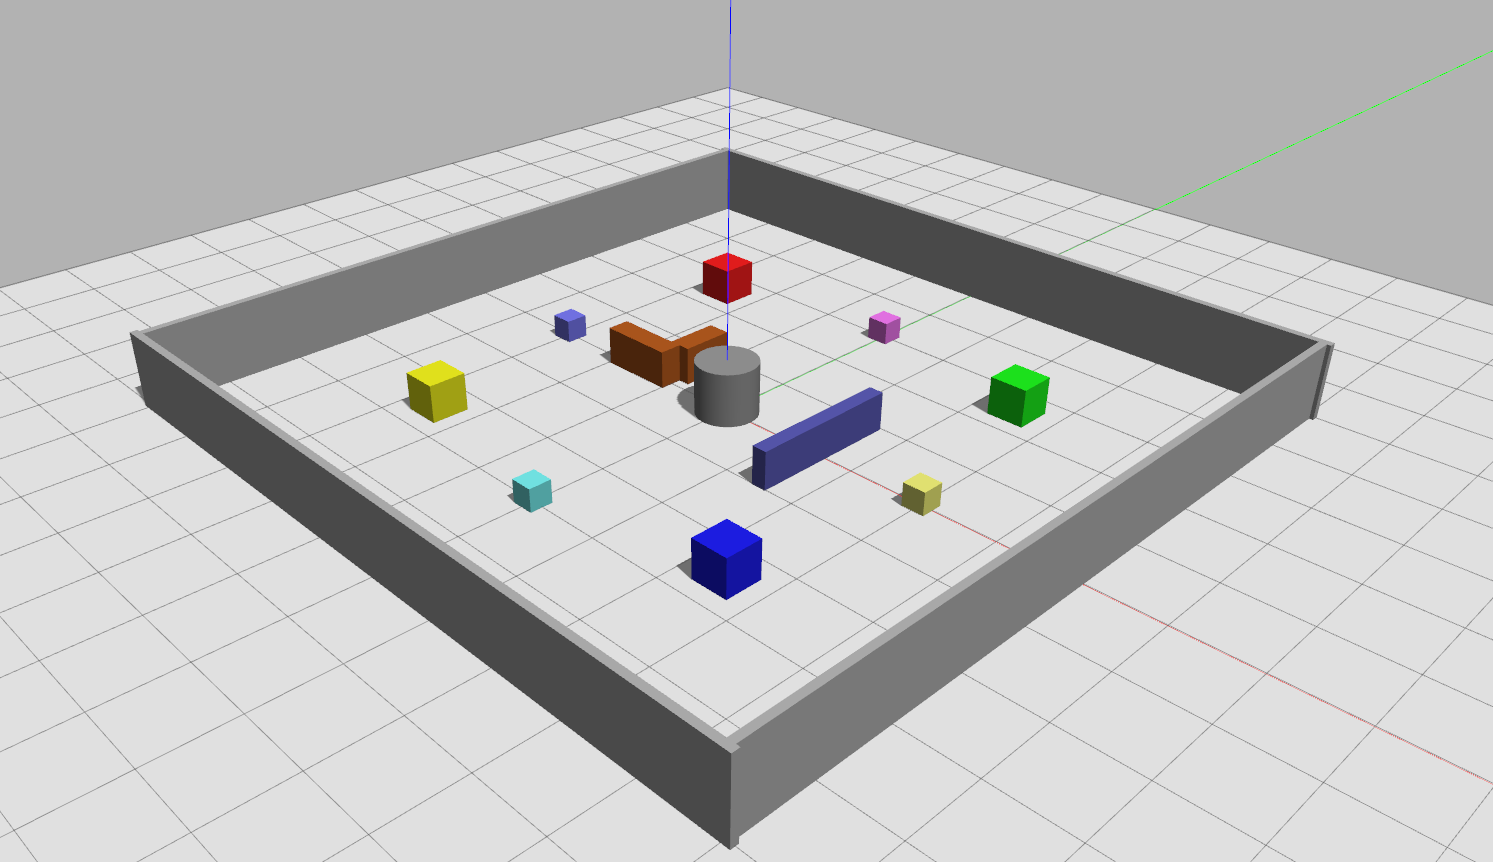
\includegraphics[width=\textwidth]{figures/Chapter 5/Room_1_simualtion.png}
        \caption{Room 1: Basic Verification}
        \label{fig:room1}
    \end{subfigure}
    \hfill
    \begin{subfigure}[b]{0.48\textwidth}
        \centering
        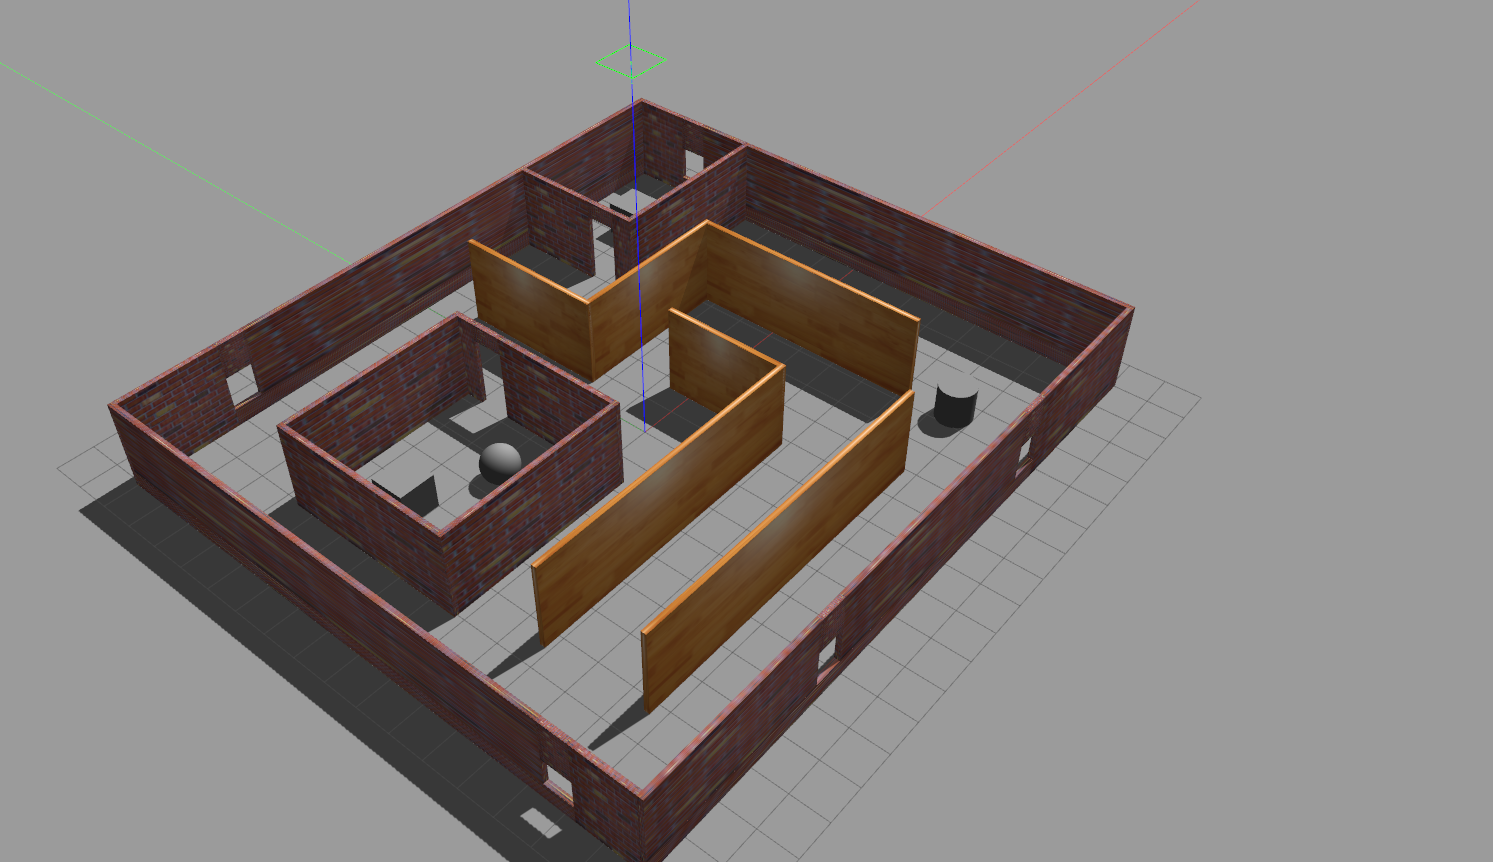
\includegraphics[width=\textwidth]{figures/Chapter 5/Room_2_simulation.png}
        \caption{Room 2: Complex Geometry}
        \label{fig:room2}
    \end{subfigure}
    \caption{Unit Testing Environments}
    \label{fig:test_rooms}
\end{figure}

\begin{figure}[H]
    \centering
    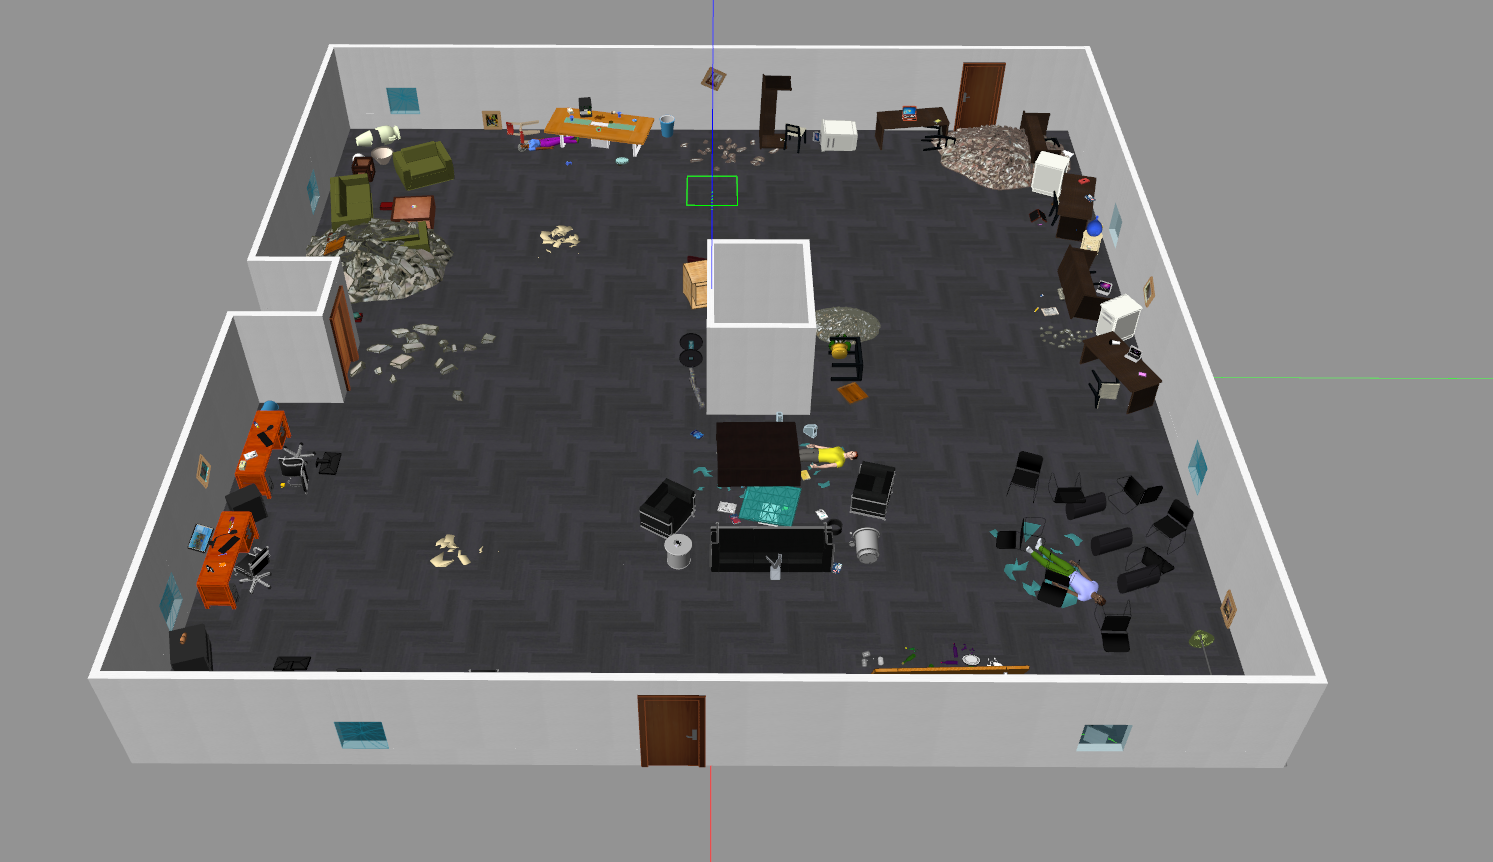
\includegraphics[width=0.9\linewidth]{figures/Chapter 5/office_earthquake_simualtion.png}
    \caption{Office Earthquake World: Disaster Response Scenario}
    \label{fig:earthquake}
\end{figure}

\begin{figure}[H]
    \centering
    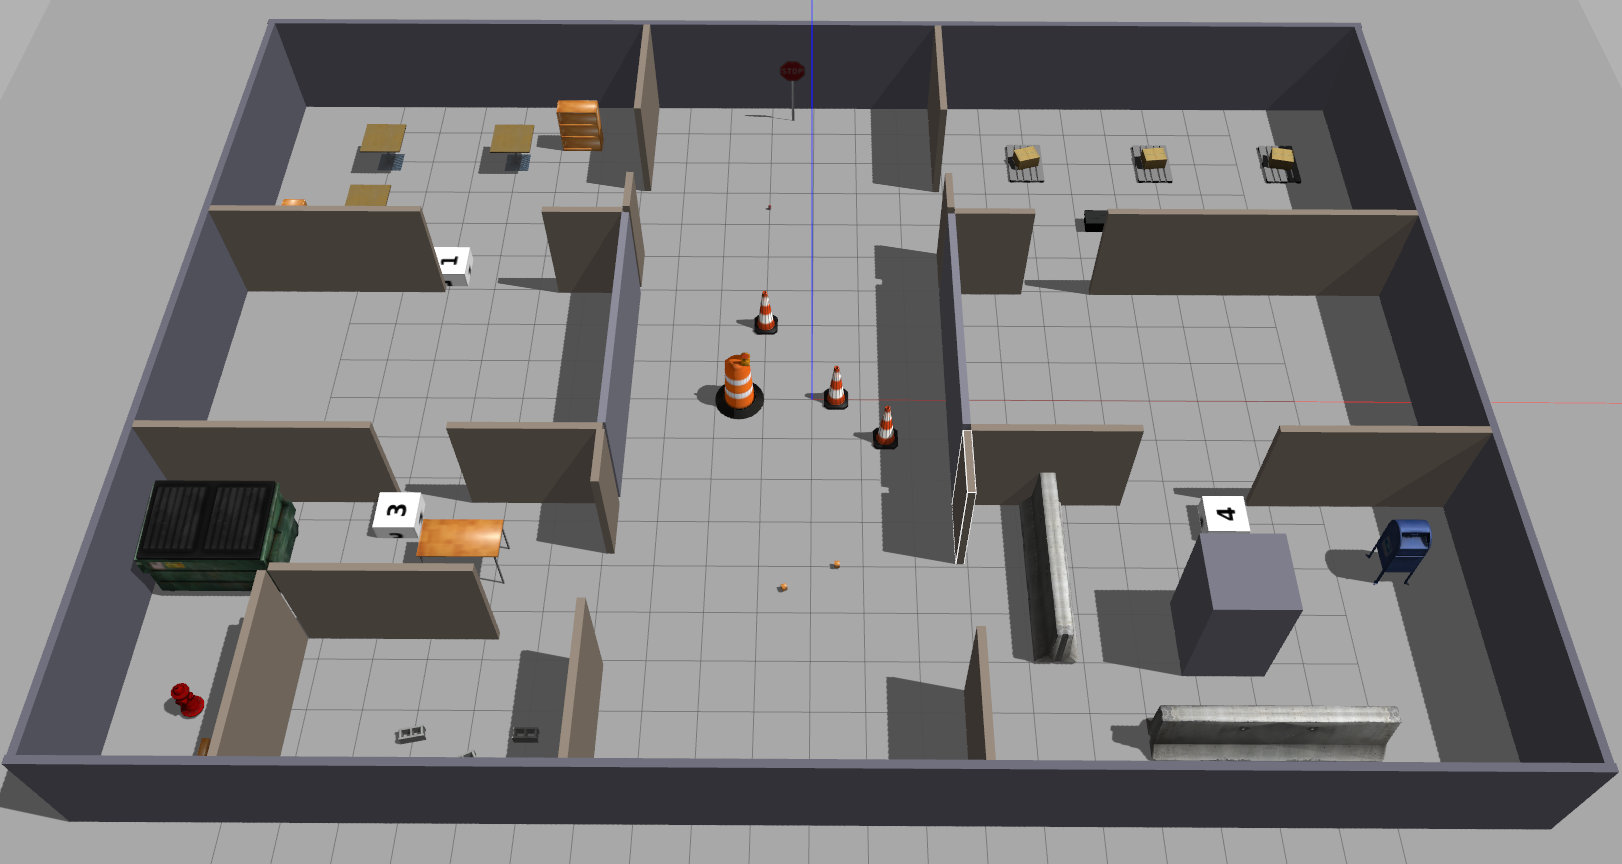
\includegraphics[width=0.9\linewidth]{figures/Chapter 5/Multi_robot_room.png}
    \caption{Multi-Robot Room: Swarm Coordination Testbed}
    \label{fig:multirobot_room}
\end{figure}

\section{Multi-Robot Swarm Architecture}
\label{sec:swarm_architecture}

Scaling from a single autonomous robot to a coordinated swarm introduces significant architectural challenges. Each robot must maintain its own independent perception, planning, and control pipeline while simultaneously participating in a shared communication network. The key enabler for this scalability is the systematic use of \textbf{namespaces}---a ROS 2 mechanism that prefixes all node names, topics, services, and TF frames with a unique identifier.

\subsection{Namespace-Based Scalability}

In ROS 2, namespaces provide logical isolation between robot instances. When a robot is launched with namespace \texttt{ausra\_1}, all its nodes and topics are automatically prefixed:

\begin{itemize}
    \item \texttt{/ausra\_1/scan} instead of \texttt{/scan}
    \item \texttt{/ausra\_1/cmd\_vel} instead of \texttt{/cmd\_vel}
    \item \texttt{/ausra\_1/odom} instead of \texttt{/odom}
    \item TF frames become \texttt{ausra\_1/base\_link}, \texttt{ausra\_1/odom}, etc.
\end{itemize}

This approach offers several critical advantages for swarm deployment:

\begin{enumerate}
    \item \textbf{Zero Code Modification:} The same Docker image, launch files, and configuration can be deployed to any number of robots by simply changing the namespace parameter
    \item \textbf{Topic Isolation:} Each robot's sensor data, control commands, and state estimates remain separate, preventing cross-contamination
    \item \textbf{TF Tree Independence:} Each robot maintains its own transform tree, avoiding the ``TF buffer collisions'' that occur when multiple robots publish to the same frame names
    \item \textbf{Selective Sharing:} Global topics (e.g., \texttt{/map}, \texttt{/swarm/status}) can remain outside namespaces for inter-robot coordination
\end{enumerate}

\begin{figure}[H]
    \centering
    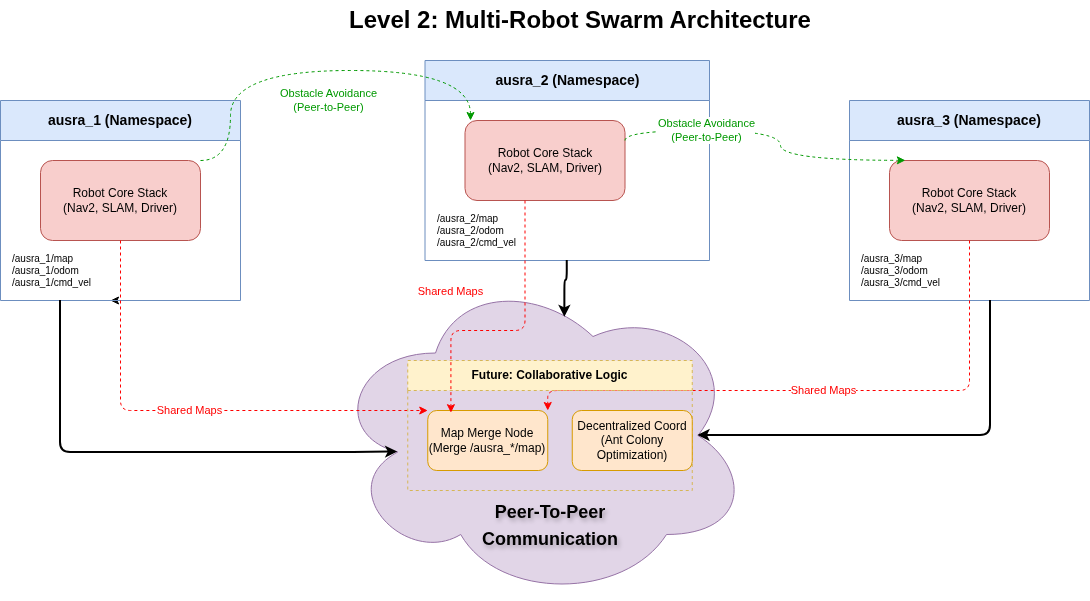
\includegraphics[width=1.0\linewidth]{figures/Chapter 5/Multi_robot_architecture.png}
    \caption{Level 2: Multi-Robot Swarm Architecture with Namespace Isolation}
    \label{fig:multi_robot_arch}
\end{figure}

\subsection{RQT Graph Analysis: Dual-Robot Operation}

Figure \ref{fig:rqt_namespace} presents the actual ROS 2 computation graph captured during simultaneous operation of two AUSRA robots (\texttt{ausra\_1} and \texttt{ausra\_2}) in Gazebo simulation. This visualization, generated using \texttt{rqt\_graph}, demonstrates the namespace isolation in practice.

\begin{figure}[H]
    \centering
    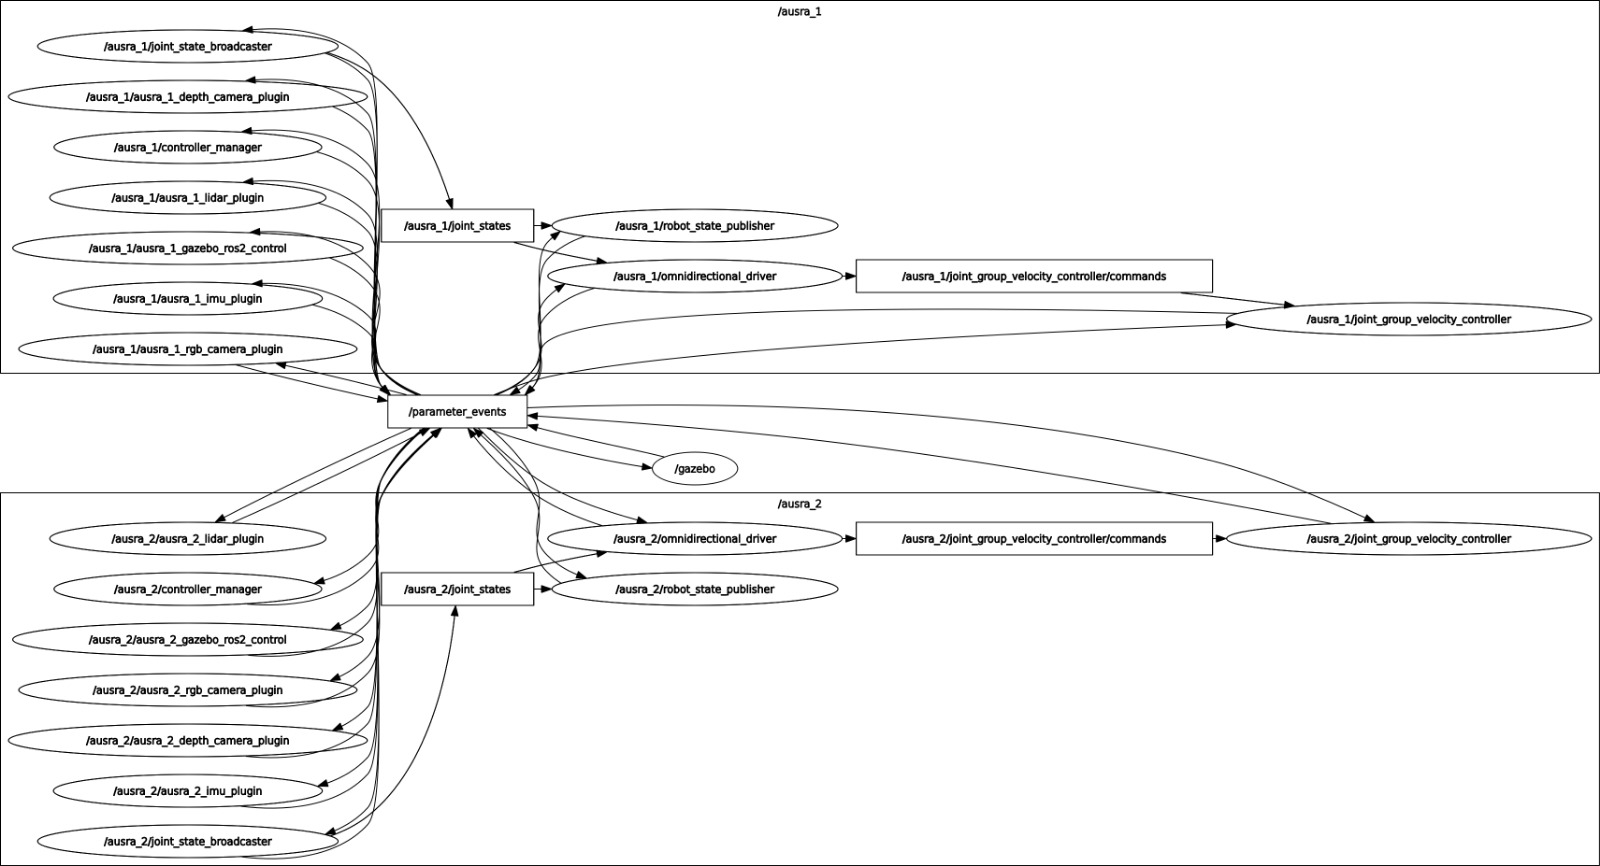
\includegraphics[width=1.0\linewidth]{figures/Chapter 5/Namespaces_of_2_robots.jpeg}
    \caption{RQT Graph: Dual-Robot Namespace Isolation During Simultaneous Operation}
    \label{fig:rqt_namespace}
\end{figure}

\subsubsection{Graph Structure Analysis}

The rqt\_graph reveals the complete node topology for both robots:

\paragraph{Per-Robot Node Set}
Each namespace contains an identical set of nodes:
\begin{itemize}
    \item \texttt{joint\_state\_broadcaster}: Publishes joint positions from Gazebo
    \item \texttt{robot\_state\_publisher}: Converts joint states to TF transforms
    \item \texttt{controller\_manager}: Manages ros2\_control lifecycle
    \item \texttt{omnidirectional\_driver}: Converts \texttt{cmd\_vel} to wheel commands
    \item \texttt{joint\_group\_velocity\_controller}: Executes wheel velocity commands
    \item Sensor plugins: \texttt{lidar\_plugin}, \texttt{imu\_plugin}, \texttt{depth\_camera\_plugin}, \texttt{rgb\_camera\_plugin}
\end{itemize}

\paragraph{Topic Flow Pattern}
The graph shows the data flow within each namespace:
\begin{enumerate}
    \item Sensor plugins publish to namespaced topics (e.g., \texttt{/ausra\_1/scan})
    \item \texttt{joint\_states} topic aggregates all joint positions
    \item \texttt{robot\_state\_publisher} broadcasts TF transforms
    \item \texttt{omnidirectional\_driver} subscribes to \texttt{cmd\_vel} and publishes to \texttt{joint\_group\_velocity\_controller/commands}
\end{enumerate}

\paragraph{Shared Resources}
Two elements remain outside namespaces:
\begin{itemize}
    \item \texttt{/gazebo}: The physics simulator node, shared by all robots
    \item \texttt{/parameter\_events}: ROS 2 system topic for parameter change notifications
\end{itemize}

\subsection{Docker-Based Swarm Deployment}

The namespace architecture integrates seamlessly with Docker containerization, enabling a ``build once, deploy everywhere'' strategy for swarm scaling.

\subsubsection{Deployment Architecture}

Each physical robot runs an identical Docker container with only one differentiating parameter:

\begin{verbatim}
# Robot 1
docker run --runtime nvidia --network host \
  -e ROBOT_NAMESPACE=ausra_1 \
  ausra_ros2:humble

# Robot 2
docker run --runtime nvidia --network host \
  -e ROBOT_NAMESPACE=ausra_2 \
  ausra_ros2:humble

# Robot N
docker run --runtime nvidia --network host \
  -e ROBOT_NAMESPACE=ausra_N \
  ausra_ros2:humble
\end{verbatim}

\subsubsection{Scalability Benefits}

This architecture provides significant operational advantages:

\begin{table}[H]
\centering
\caption{Docker + Namespace Scalability Benefits}
\label{tab:docker_scalability}
\begin{tabular}{|l|p{9cm}|}
\hline
\textbf{Benefit} & \textbf{Description} \\
\hline
Identical Images & Single Docker image for entire swarm; no per-robot customization \\
\hline
Rapid Deployment & New robots join swarm in seconds via container launch \\
\hline
Version Consistency & All robots run identical software versions, eliminating ``works on my robot'' issues \\
\hline
Easy Updates & Push new image to registry; all robots pull and restart \\
\hline
Failure Isolation & Container crash affects only one robot; others continue operating \\
\hline
Resource Management & Docker limits CPU/memory per robot, preventing runaway processes \\
\hline
\end{tabular}
\end{table}

\subsubsection{Launch File Integration}

The launch system automatically applies namespaces to all nodes:

\begin{verbatim}
# In launch file
namespace = LaunchConfiguration('robot_namespace')

Node(
    package='slam_toolbox',
    executable='async_slam_toolbox_node',
    namespace=namespace,
    parameters=[{'use_sim_time': True}],
    remappings=[('/tf', 'tf'), ('/tf_static', 'tf_static')]
)
\end{verbatim}

The \texttt{remappings} ensure TF topics remain global for multi-robot SLAM coordination while all other topics are namespaced.

\subsection{Swarm Communication Topology}

With namespace isolation established, robots communicate through two distinct channels:

\begin{enumerate}
    \item \textbf{Namespaced Topics:} Robot-specific data (sensor readings, local state)
    \item \textbf{Global Topics:} Swarm-level coordination (task allocation, shared map, inter-robot poses)
\end{enumerate}

\begin{table}[H]
\centering
\caption{Topic Namespace Strategy}
\label{tab:topic_namespace}
\begin{tabular}{|l|l|l|}
\hline
\textbf{Topic Type} & \textbf{Example} & \textbf{Namespace} \\
\hline
Sensor Data & \texttt{/ausra\_1/scan} & Per-robot \\
Odometry & \texttt{/ausra\_1/odom} & Per-robot \\
Control Commands & \texttt{/ausra\_1/cmd\_vel} & Per-robot \\
Robot Pose Broadcast & \texttt{/swarm/poses} & Global \\
Task Allocation & \texttt{/swarm/tasks} & Global \\
Merged Map & \texttt{/map} & Global \\
Emergency Stop & \texttt{/swarm/estop} & Global \\
\hline
\end{tabular}
\end{table}

\section{Communication Stack}
\label{sec:communication}

\subsection{DDS Middleware Configuration}

ROS 2 communication relies on the Data Distribution Service (DDS) middleware. For swarm operation, proper DDS configuration is critical:

\begin{itemize}
    \item \textbf{Discovery:} Automatic peer discovery via multicast (requires \texttt{network\_mode: host} in Docker)
    \item \textbf{Domain ID:} All swarm robots share the same \texttt{ROS\_DOMAIN\_ID} for mutual visibility
    \item \textbf{QoS Profiles:} Configured per-topic based on reliability requirements
\end{itemize}

\subsection{Quality of Service Configuration}

\begin{table}[H]
\centering
\caption{QoS Configuration by Topic Type}
\label{tab:qos_config}
\begin{tabular}{|l|c|c|c|}
\hline
\textbf{Topic} & \textbf{Reliability} & \textbf{Durability} & \textbf{History} \\
\hline
/scan, /imu & Best Effort & Volatile & Keep Last (5) \\
/cmd\_vel & Reliable & Volatile & Keep Last (1) \\
/map & Reliable & Transient Local & Keep Last (1) \\
/swarm/tasks & Reliable & Transient Local & Keep All \\
/tf & Reliable & Volatile & Keep Last (100) \\
\hline
\end{tabular}
\end{table}

\subsection{Inter-Robot Communication}

Communication between robots is achieved through the shared DDS network:

\begin{itemize}
    \item \textbf{Transport:} WiFi-based UDP/TCP with automatic failover
    \item \textbf{Middleware:} Cyclone DDS (default for ROS 2 Humble) with tuned buffer sizes
    \item \textbf{Message Types:}
    \begin{itemize}
        \item \texttt{geometry\_msgs/PoseStamped}: Robot pose broadcasts at 10 Hz
        \item \texttt{nav\_msgs/OccupancyGrid}: Map sharing for collaborative SLAM
        \item \texttt{std\_msgs/String}: Task allocation and status messages
    \end{itemize}
\end{itemize}

% Add your detailed content here...

\section{The Autonomous System}
\label{sec:autonomous_system}

\subsection{Sensor Fusion and Localization}
\label{subsec:localization}

Accurate state estimation requires fusing multiple sensors with complementary characteristics. Wheel encoders provide good short-term position estimates but suffer from cumulative drift. The IMU provides excellent short-term orientation but drifts over longer periods. The Extended Kalman Filter (EKF) produces optimal estimates more accurate than any single sensor.

\subsubsection{Extended Kalman Filter Architecture}

The \texttt{robot\_localization} package implements the EKF for sensor fusion, configured via \texttt{ekf.yaml}:

\paragraph{State Vector}
\begin{equation}
\mathbf{x} = [x, y, z, \phi, \theta, \psi, \dot{x}, \dot{y}, \dot{z}, \dot{\phi}, \dot{\theta}, \dot{\psi}, \ddot{x}, \ddot{y}, \ddot{z}]^T
\label{eq:state_vector}
\end{equation}

\paragraph{Sensor Configuration}
\begin{itemize}
    \item \textbf{Wheel Odometry (50 Hz):} Provides $x$, $y$ position and $\psi$ (yaw) orientation
    \item \textbf{IMU (100 Hz):} Provides angular velocity ($\dot{\phi}, \dot{\theta}, \dot{\psi}$) and linear acceleration ($\ddot{x}, \ddot{y}, \ddot{z}$)
    \item \textbf{Visual Odometry (10--30 Hz):} Validates wheel data during slip conditions
\end{itemize}

\paragraph{Covariance Tuning}
Process noise and sensor covariances critically affect filter performance:
\begin{itemize}
    \item \textbf{IMU Angular Velocity:} 0.001 (rad/s)$^2$ diagonal covariance
    \item \textbf{IMU Linear Acceleration:} 0.01 (m/s$^2$)$^2$ diagonal covariance
    \item \textbf{Wheel Odometry Position:} Values tuned based on encoder resolution and wheel slip characteristics
\end{itemize}

\subsubsection{ROS 2 IMU Driver Implementation}

The \texttt{imu\_esp32\_bridge} package provides the bridge between hardware and ROS 2:

\paragraph{Topics Published}
\begin{itemize}
    \item \texttt{/imu/data\_raw}: Combined accelerometer/gyroscope data (\texttt{sensor\_msgs/Imu})
    \item \texttt{/imu/mag}: Magnetometer data (\texttt{sensor\_msgs/MagneticField})
\end{itemize}

\paragraph{Unit Conversions}
\begin{itemize}
    \item Accelerometer: $g \rightarrow$ m/s$^2$ (multiply by 9.81)
    \item Gyroscope: °/s $\rightarrow$ rad/s (multiply by $\pi$/180)
    \item Magnetometer: $\mu$T $\rightarrow$ T (multiply by $10^{-6}$)
\end{itemize}

\begin{figure}[H]
    \centering
    \begin{subfigure}[b]{0.45\textwidth}
        \centering
        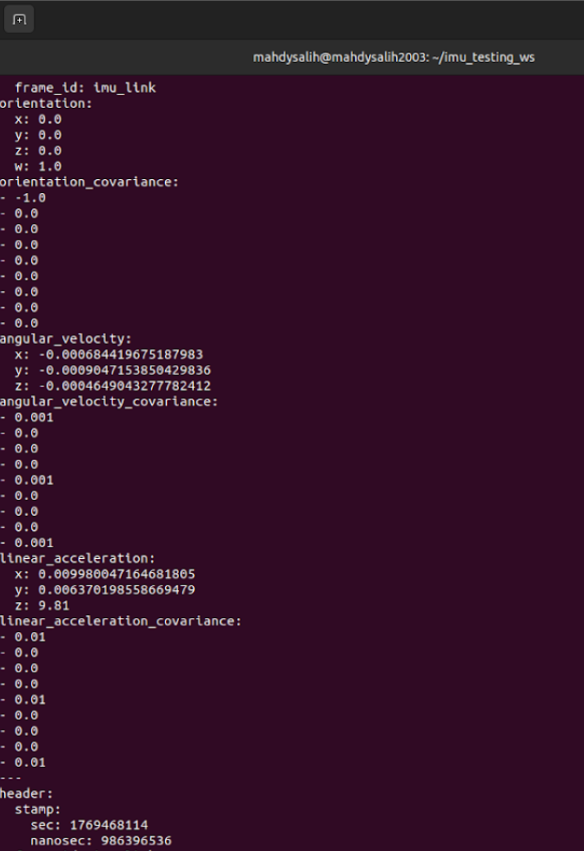
\includegraphics[width=\linewidth]{figures/Chapter 5/IMU_terminal.png}
        \caption{IMU Data Stream}
        \label{fig:imu_terminal}
    \end{subfigure}
    \hfill
    \begin{subfigure}[b]{0.45\textwidth}
        \centering
        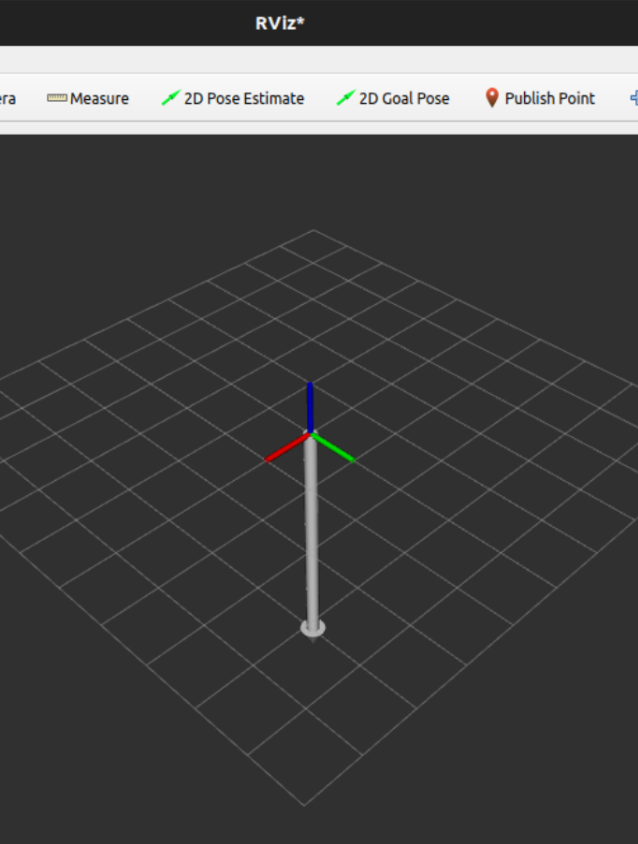
\includegraphics[width=\linewidth]{figures/Chapter 5/IMU_rviz.png}
        \caption{IMU Visualization in RViz2}
        \label{fig:imu_rviz}
    \end{subfigure}
    \caption{IMU Data Acquisition and Visualization}
    \label{fig:imu_data}
\end{figure}

\subsubsection{Visualization and Validation}

\begin{figure}[H]
    \centering
    \begin{subfigure}[b]{0.45\textwidth}
        \centering
        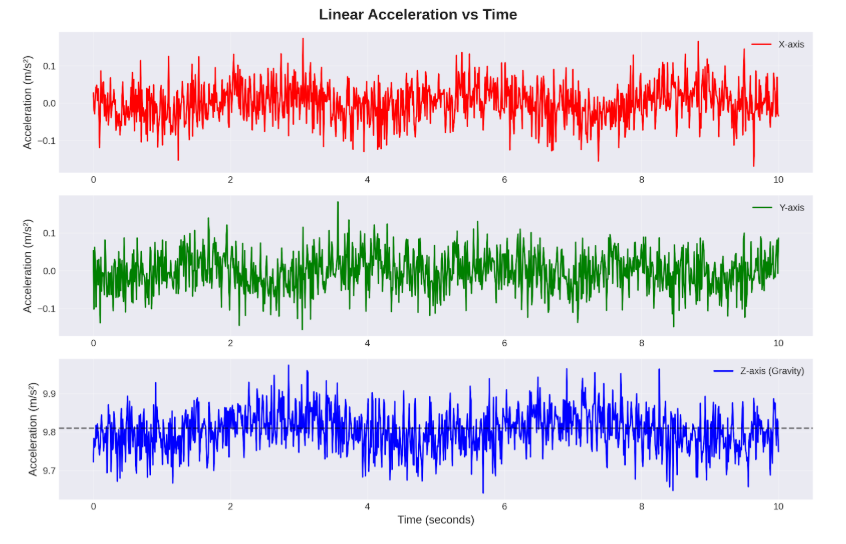
\includegraphics[width=\linewidth]{figures/Chapter 5/Linear_acc.png}
        \caption{Linear Acceleration (Z-axis showing gravity)}
        \label{fig:linear_acc}
    \end{subfigure}
    \hfill
    \begin{subfigure}[b]{0.45\textwidth}
        \centering
        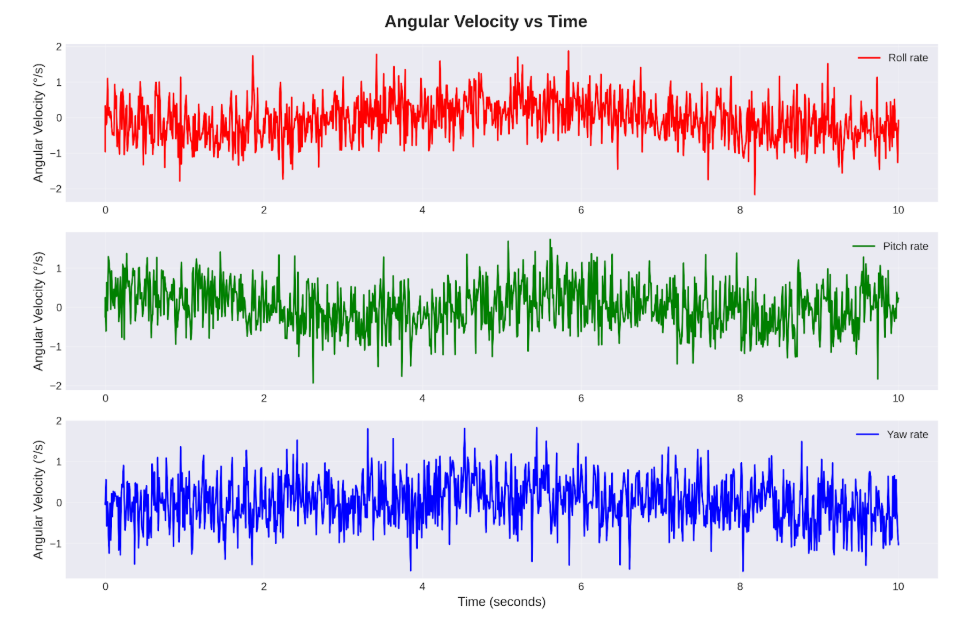
\includegraphics[width=\linewidth]{figures/Chapter 5/Angular_vel.png}
        \caption{Angular Velocity During Rotation}
        \label{fig:angular_vel}
    \end{subfigure}
    \caption{IMU Sensor Measurements}
    \label{fig:imu_measurements}
\end{figure}

Key observations from visualization analysis:
\begin{itemize}
    \item Noise characteristics validate EKF covariance parameters
    \item Absence of systematic drift confirms calibration effectiveness
    \item Clear gravity measurement ($\approx$9.81 m/s$^2$ on Z-axis) demonstrates adequate sensor performance
\end{itemize}

\subsubsection{Direct Jetson Integration}

For production deployment, direct Jetson Orin Nano integration eliminates the ESP32 bridge:
\begin{itemize}
    \item \textbf{Latency Reduction:} 35--55 ms improvement (from 58 ms to 14 ms end-to-end)
    \item \textbf{Simplified Architecture:} Eliminates USB serial communication overhead
    \item \textbf{I2C Connection:} Pins 3 (SDA) and 5 (SCL) on Jetson 40-pin header at 400 kHz
\end{itemize}

\subsubsection{SLAM Integration}

\paragraph{The Navigation Problem}
Autonomous navigation in unknown environments requires solving three interdependent problems:
\begin{enumerate}
    \item \textbf{Localization:} Continuous pose estimation relative to a reference frame
    \item \textbf{Mapping:} Constructing an environment representation for obstacle identification
    \item \textbf{Path Planning:} Calculating safe, efficient trajectories dependent on both localization and mapping
\end{enumerate}

\paragraph{Challenges in Unstructured Environments}
Real-world environments present unique challenges:
\begin{itemize}
    \item \textbf{Unstructured Geometry:} Irregular shapes and unexpected obstacles
    \item \textbf{GPS-Denied Operation:} Indoor and underground areas require internal sensors for localization
    \item \textbf{Kinematic Instability:} Wheel slippage invalidates dead reckoning
\end{itemize}

\paragraph{SLAM: Simultaneous Localization and Mapping}
SLAM addresses the fundamental interdependence: accurate mapping requires known position, while localization requires a reference map. The algorithm constructs a map while determining the robot's location within it.

SLAM is formulated as a probabilistic problem, estimating the posterior probability distribution of the robot's path and map given noisy sensor data.

\subsection{Mapping with slam\_toolbox}
\label{subsec:slam_toolbox}

The \texttt{slam\_toolbox} package is a graph-based SLAM framework for ROS 2, selected for its robust loop closure, efficient optimization, and tight ROS 2 integration. Alternative approaches such as GMapping \cite{grisetti2007improved} and Google Cartographer \cite{hess2016cartographer} were evaluated but ultimately \texttt{slam\_toolbox} was chosen for its superior performance in dynamic environments.

\subsubsection{Algorithm Selection}

\begin{table}[H]
\centering
\caption{SLAM Algorithm Selection Matrix}
\label{tab:slam_selection}
\begin{tabular}{|l|c|c|c|c|c|c|c|}
\hline
\textbf{Criteria} & \textbf{Weight} & \multicolumn{2}{c|}{\textbf{slam\_toolbox}} & \multicolumn{2}{c|}{\textbf{Gmapping}} & \multicolumn{2}{c|}{\textbf{Hector}} \\
\cline{3-8}
 & & Rate & Score & Rate & Score & Rate & Score \\
\hline
Sensor Fusion & 5 & 4 & 20 & 5 & 25 & 0 & 0 \\
\hline
Loop Closure & 5 & 5 & 25 & 1 & 5 & 0 & 0 \\
\hline
Indoor Suitability & 5 & 5 & 25 & 4 & 20 & 4 & 20 \\
\hline
Map Sharpness & 4 & 4 & 16 & 3 & 12 & 5 & 20 \\
\hline
ROS 2 Maturity & 4 & 5 & 20 & 1 & 4 & 2 & 8 \\
\hline
Computational Cost & 3 & 4 & 12 & 4 & 12 & 5 & 15 \\
\hline
\textbf{Final Score} & & & \textbf{118} & & \textbf{78} & & \textbf{63} \\
\hline
\end{tabular}
\end{table}

\subsubsection{System Architecture}

\begin{figure}[H]
    \centering
    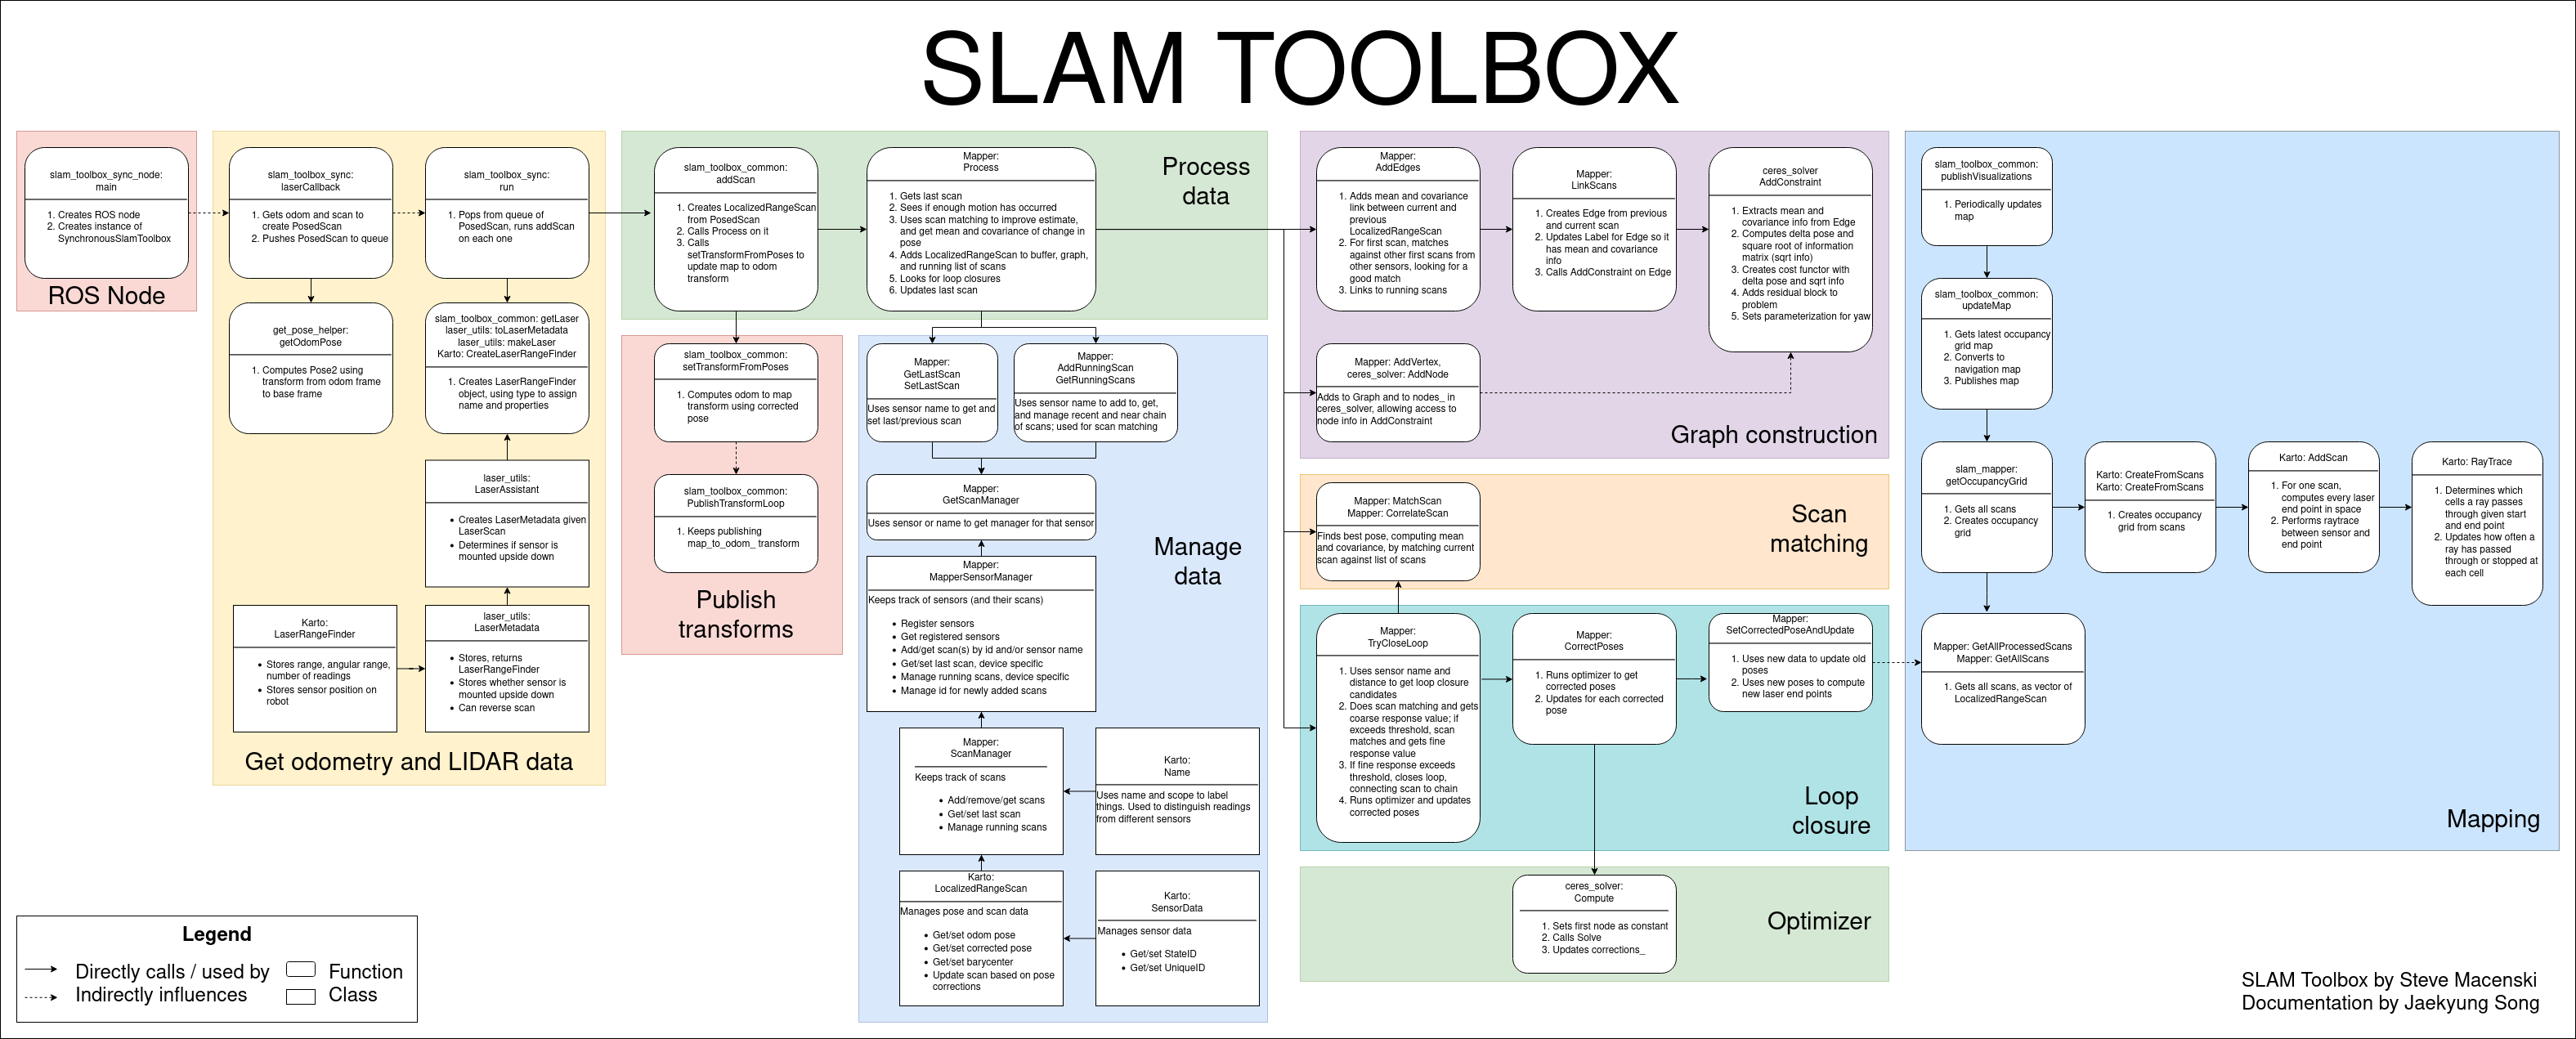
\includegraphics[width=0.85\linewidth]{figures/Chapter 5/slam_toolbox_sync.png}
    \caption{slam\_toolbox System Architecture}
    \label{fig:slam_toolbox_arch}
\end{figure}

The pipeline consists of:
\begin{enumerate}
    \item \textbf{Sensor Data Acquisition:} LiDAR scans and odometry input
    \item \textbf{Pose Graph Construction:} Nodes represent poses, edges encode constraints
    \item \textbf{Scan Matching:} Aligns consecutive scans for relative motion
    \item \textbf{Loop Closure Detection:} Identifies previously visited locations
    \item \textbf{Graph Optimization:} Minimizes constraint errors using Ceres Solver
    \item \textbf{Map Generation:} Outputs occupancy grid
\end{enumerate}

\paragraph{Pose Graph Representation}
Each node represents robot pose $\mathbf{x}_i = [x_i, y_i, \theta_i]^T$. Edges encode relative measurements:
\begin{equation}
\mathbf{z}_{ij} = \mathbf{x}_j \ominus \mathbf{x}_i
\label{eq:relative_pose}
\end{equation}

\paragraph{Maximum Likelihood Formulation}
The optimization minimizes:
\begin{equation}
\mathbf{X}^* = \arg\min_{\mathbf{X}} \sum_{(i,j) \in E} \|\mathbf{z}_{ij} - h(\mathbf{x}_i, \mathbf{x}_j)\|^2_{\Omega_{ij}}
\label{eq:slam_optimization}
\end{equation}
where $\Omega_{ij}$ is the information matrix weighting constraint confidence.

\subsubsection{ROS 2 Topics and Frames}

\begin{table}[H]
\centering
\caption{slam\_toolbox ROS 2 Interface}
\label{tab:slam_topics}
\begin{tabular}{|l|l|l|}
\hline
\textbf{Topic} & \textbf{Type} & \textbf{Description} \\
\hline
/scan & sensor\_msgs/LaserScan & LiDAR input \\
/odom & nav\_msgs/Odometry & Wheel odometry \\
/map & nav\_msgs/OccupancyGrid & Output map \\
/tf & tf2\_msgs/TFMessage & Coordinate transforms \\
\hline
\end{tabular}
\end{table}

Transform chain: \texttt{map} $\rightarrow$ \texttt{odom} (from slam\_toolbox) $\rightarrow$ \texttt{base\_link} (from EKF).

\subsubsection{Parameter Tuning Strategy}

Parameters were tuned to address specific mapping artifacts:

\paragraph{Wall Thickness Reduction}
Excessive wall thickness results from pose estimation errors. Scan matching precision was increased, and occupancy probability thresholds were tuned.

\begin{figure}[H]
    \centering
    \begin{subfigure}[b]{0.45\textwidth}
        \centering
        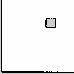
\includegraphics[width=\linewidth]{figures/Chapter 5/wall_thickness_before.png}
        \caption{Before Tuning}
        \label{fig:wall_thick_before}
    \end{subfigure}
    \hfill
    \begin{subfigure}[b]{0.45\textwidth}
        \centering
        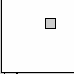
\includegraphics[width=\linewidth]{figures/Chapter 5/wall_thickness_after.png}
        \caption{After Tuning}
        \label{fig:wall_thick_after}
    \end{subfigure}
    \caption{Wall Thickness Optimization}
    \label{fig:wall_thickness}
\end{figure}

\paragraph{Corner Preservation}
Wall discontinuities occur with insufficient scan matching confidence. Angle variance penalties were increased to prevent corner deformation.

\begin{figure}[H]
    \centering
    \begin{subfigure}[b]{0.45\textwidth}
        \centering
        
\includegraphics[width=\linewidth]{figures/Chapter 5/wall_discontinuity_before.png}
        \caption{Before Tuning}
        \label{fig:corner_before}
    \end{subfigure}
    \hfill
    \begin{subfigure}[b]{0.45\textwidth}
        \centering
        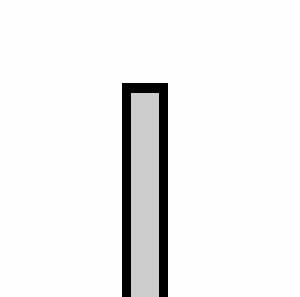
\includegraphics[width=\linewidth]{figures/Chapter 5/wall_discontinuity_after.png}
        \caption{After Tuning}
        \label{fig:corner_after}
    \end{subfigure}
    \caption{Corner Preservation Optimization}
    \label{fig:corner_preservation}
\end{figure}

\subsubsection{Experimental Results}

\begin{figure}[H]
    \centering
    \begin{subfigure}[b]{0.45\textwidth}
        \centering
        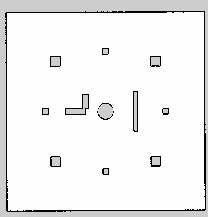
\includegraphics[width=\linewidth]{figures/Chapter 5/room1_map_trial3.png}
        \caption{Single Room Environment}
        \label{fig:room1_map}
    \end{subfigure}
    \hfill
    \begin{subfigure}[b]{0.45\textwidth}
        \centering
        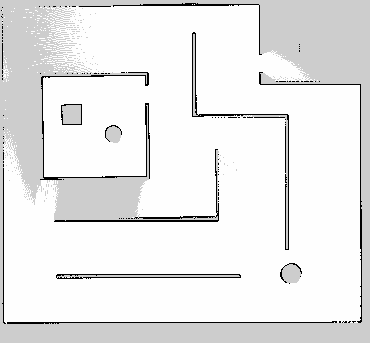
\includegraphics[width=\linewidth]{figures/Chapter 5/room2_map_trial1.png}
        \caption{Corridor Environment}
        \label{fig:room2_map}
    \end{subfigure}
    \caption{slam\_toolbox Mapping Results}
    \label{fig:slam_results}
\end{figure}

\begin{figure}[H]
    \centering
    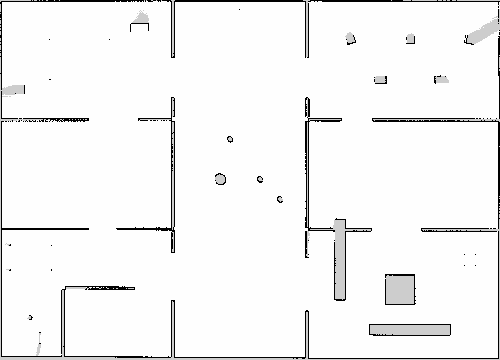
\includegraphics[width=0.7\linewidth]{figures/Chapter 5/multirobot_room_map.png}
    \caption{Multi-Room Environment Mapping}
    \label{fig:multiroom_map}
\end{figure}

The generated maps exhibit clear wall boundaries, consistent room shapes, and minimal drift after loop closure.

\subsection{Google Cartographer SLAM}
\label{subsec:cartographer}

Google Cartographer was evaluated as an alternative graph-based SLAM framework with advanced loop closure capabilities.

\subsubsection{Algorithm Selection}

\begin{table}[H]
\centering
\caption{Cartographer Selection Matrix}
\label{tab:cartographer_selection}
\begin{tabular}{|l|c|c|c|c|c|c|c|}
\hline
\textbf{Criteria} & \textbf{Weight} & \multicolumn{2}{c|}{\textbf{Cartographer}} & \multicolumn{2}{c|}{\textbf{Gmapping}} & \multicolumn{2}{c|}{\textbf{Hector}} \\
\cline{3-8}
 & & Rate & Score & Rate & Score & Rate & Score \\
\hline
Sensor Fusion & 5 & 5 & 25 & 5 & 25 & 0 & 0 \\
\hline
Loop Closure & 5 & 5 & 25 & 1 & 5 & 0 & 0 \\
\hline
Indoor Suitability & 5 & 5 & 25 & 4 & 20 & 4 & 20 \\
\hline
Map Sharpness & 4 & 5 & 20 & 3 & 12 & 5 & 20 \\
\hline
ROS 2 Maturity & 4 & 5 & 20 & 1 & 4 & 2 & 8 \\
\hline
Computational Cost & 3 & 3 & 9 & 4 & 12 & 5 & 15 \\
\hline
\textbf{Final Score} & & & \textbf{124} & & \textbf{78} & & \textbf{63} \\
\hline
\end{tabular}
\end{table}

\subsubsection{System Architecture}

\begin{figure}[H]
    \centering
    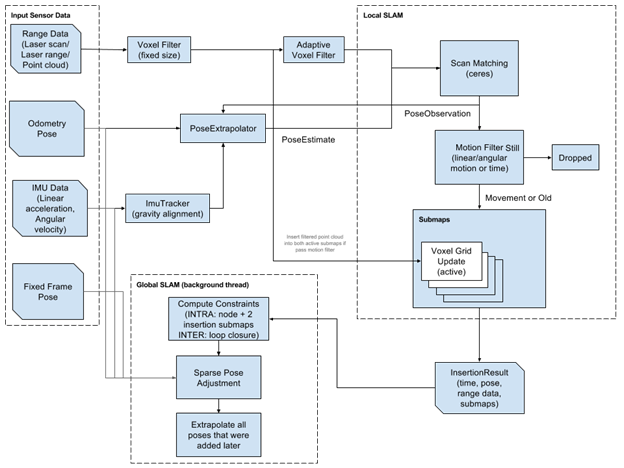
\includegraphics[width=0.9\linewidth]{figures/Chapter 5/cartographer_architecture.png}
    \caption{Google Cartographer Architecture}
    \label{fig:cartographer_arch}
\end{figure}

Cartographer operates with two asynchronous subsystems:
\begin{itemize}
    \item \textbf{Local SLAM (Front-End):} Processes sensor data for immediate trajectory estimation using submaps
    \item \textbf{Global SLAM (Back-End):} Optimizes the pose graph to correct long-term drift
\end{itemize}

\paragraph{Input Data}
\begin{itemize}
    \item \textbf{Range Data:} 2D LiDAR scans
    \item \textbf{Odometry:} Wheel encoder data ($v_x$, $v_y$, $\omega$)
    \item \textbf{IMU:} Angular velocity and linear acceleration for gravity alignment
\end{itemize}

\subsubsection{Local SLAM: Trajectory Builder}

\paragraph{Probability Grids}
Unlike binary maps, Cartographer uses probability grids where each cell stores obstruction likelihood. Laser hits increase probability; passes decrease it.

\paragraph{Ceres Scan Matching}
The solver minimizes:
\begin{equation}
J(\xi) = \underbrace{\sum_{k=1}^{K} (1 - M_{smooth}(T_{\xi} h_k))^2}_{\text{Scan Match Cost}} + \underbrace{\lambda_t \|T_{\xi} - \xi_{odom}\|^2}_{\text{Translation Penalty}} + \underbrace{\lambda_r \|\theta_{\xi} - \theta_{odom}\|^2}_{\text{Rotation Penalty}}
\label{eq:ceres_cost}
\end{equation}
where $M_{smooth}$ is the interpolated map probability, and $\lambda_t$, $\lambda_r$ are trust weights.

\subsubsection{Global SLAM: Pose Graph Optimization}

\paragraph{Loop Closure via Branch-and-Bound}
Cartographer uses Branch-and-Bound to efficiently search for loop closures, discarding regions where the best possible match score is below threshold.

\paragraph{Sparse Pose Adjustment}
The optimizer minimizes total error energy:
\begin{equation}
\arg\min \sum_{ij} \mathbf{e}_{ij}^T \Omega_{ij} \mathbf{e}_{ij}
\label{eq:spa}
\end{equation}
where $\mathbf{e}_{ij}$ is the error between measured and estimated relative poses.

\subsubsection{Error Diagnosis and Tuning}

\paragraph{Odometry Drift Correction}

\begin{figure}[H]
    \centering
    \begin{subfigure}[b]{0.45\textwidth}
        \centering
        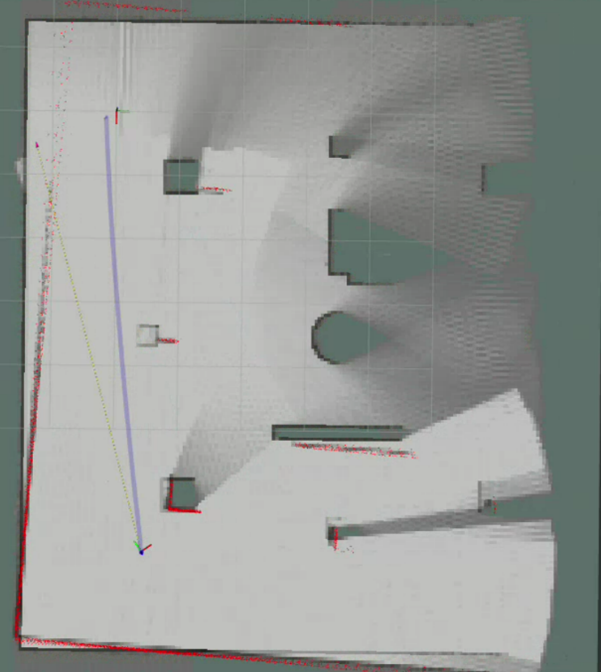
\includegraphics[width=\linewidth]{figures/Chapter 5/initial_odom_drift.png}
        \caption{Initial Drift}
        \label{fig:odom_drift}
    \end{subfigure}
    \hfill
    \begin{subfigure}[b]{0.45\textwidth}
        \centering
        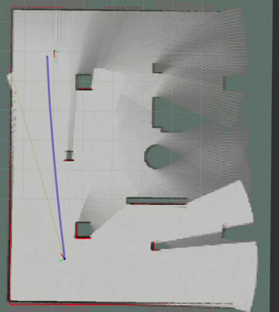
\includegraphics[width=\linewidth]{figures/Chapter 5/snap_correction.png}
        \caption{After Global Correction}
        \label{fig:snap_correction}
    \end{subfigure}
    \caption{Odometry Drift and Correction}
    \label{fig:drift_correction}
\end{figure}

\paragraph{Lateral Slip Compensation}
Omni-wheels cause lateral slip, producing ``ghosting'' artifacts. The Real-Time Correlative Scan Matcher was enabled with a 0.1m linear and 40° angular search window.

\begin{figure}[H]
    \centering
    \begin{subfigure}[b]{0.45\textwidth}
        \centering
        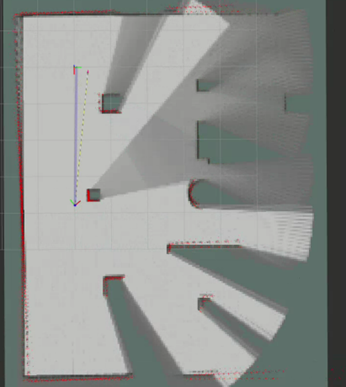
\includegraphics[width=\linewidth]{figures/Chapter 5/ghosting_problem.png}
        \caption{Ghosting Artifact}
        \label{fig:ghosting}
    \end{subfigure}
    \hfill
    \begin{subfigure}[b]{0.45\textwidth}
        \centering
        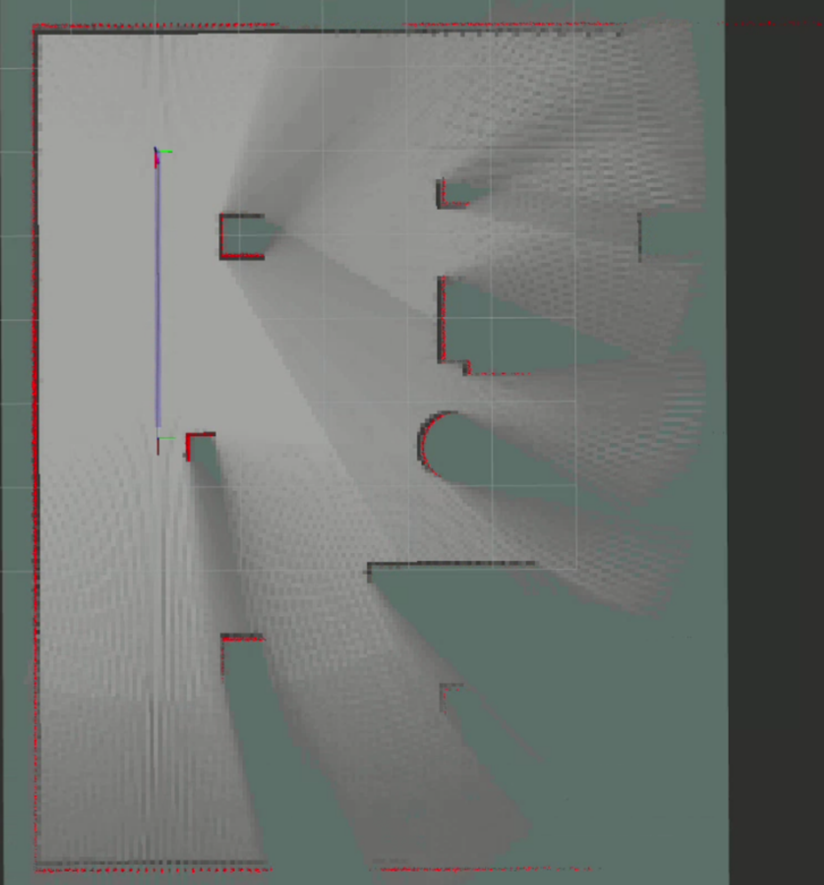
\includegraphics[width=\linewidth]{figures/Chapter 5/solved_ghosting.png}
        \caption{After Tuning}
        \label{fig:solved_ghosting}
    \end{subfigure}
    \caption{Lateral Slip Artifact Correction}
    \label{fig:ghosting_fix}
\end{figure}

\subsubsection{Final Configuration Parameters}

Key tuning parameters:
\begin{itemize}
    \item \textbf{Correlative Scan Matcher:} Enabled with 0.1m/40° search window
    \item \textbf{Ceres Weights:} Occupied space: 20, Translation: 10, Rotation: 40
    \item \textbf{Submaps:} 35 scans per submap for stability
    \item \textbf{Miss Probability:} 0.49 (conservative erasing)
    \item \textbf{Optimization Frequency:} Every 20 nodes
\end{itemize}

\subsubsection{Validation Results}

\begin{figure}[H]
    \centering
    \begin{subfigure}[b]{0.45\textwidth}
        \centering
        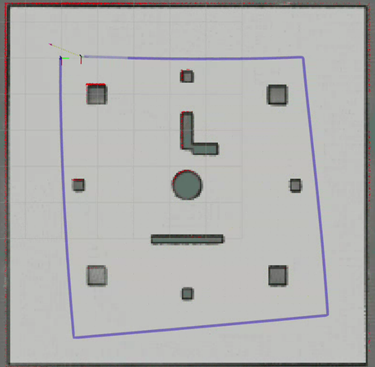
\includegraphics[width=\linewidth]{figures/Chapter 5/loop_closure_before.png}
        \caption{Before Loop Closure}
        \label{fig:loop_before}
    \end{subfigure}
    \hfill
    \begin{subfigure}[b]{0.45\textwidth}
        \centering
        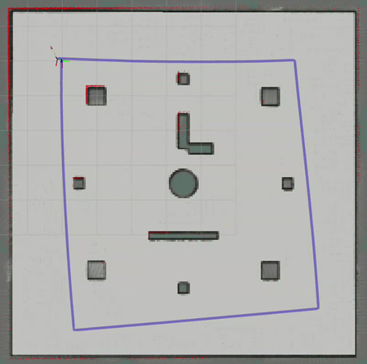
\includegraphics[width=\linewidth]{figures/Chapter 5/loop_closure_after.png}
        \caption{After Loop Closure}
        \label{fig:loop_after}
    \end{subfigure}
    \caption{Loop Closure Correction}
    \label{fig:loop_closure_results}
\end{figure}

\begin{figure}[H]
    \centering
    \begin{subfigure}[b]{0.45\textwidth}
        \centering
        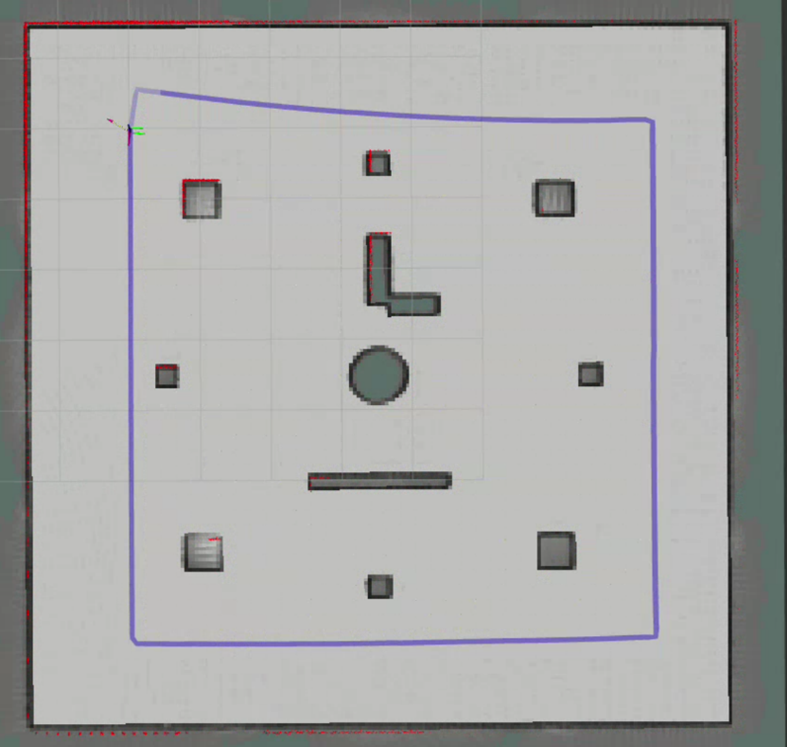
\includegraphics[width=\linewidth]{figures/Chapter 5/final tuned map.png}
        \caption{Tuned Navigation Map}
        \label{fig:final_map}
    \end{subfigure}
    \hfill
    \begin{subfigure}[b]{0.45\textwidth}
        \centering
        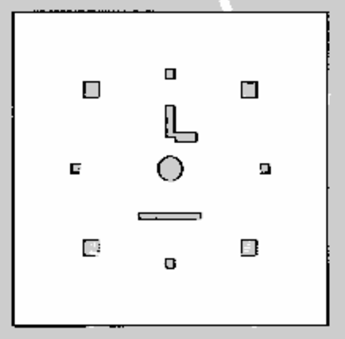
\includegraphics[width=\linewidth]{figures/Chapter 5/final_occupancy_grid_map.png}
        \caption{Final Occupancy Grid}
        \label{fig:final_grid}
    \end{subfigure}
    \caption{Cartographer Final Mapping Results}
    \label{fig:cartographer_results}
\end{figure}

\subsection{SLAM Framework Selection}
\label{subsec:slam_selection}

Both frameworks were evaluated under identical conditions. While Cartographer achieves high accuracy, it exhibited increased computational demand during loop closure and sensitivity to odometry noise and parameter tuning.

\texttt{slam\_toolbox} consistently produced maps with improved structural clarity, reduced wall thickening, and fewer alignment artifacts, indicating more effective scan-to-map alignment in the presence of sensor noise.

Based on the evaluation, \textbf{slam\_toolbox} was selected as the primary SLAM solution for:
\begin{itemize}
    \item \textbf{Map Quality:} Superior structural clarity
    \item \textbf{Computational Efficiency:} Lower resource requirements
    \item \textbf{Odometry Drift Correction:} Better handling of omni-directional kinematics
\end{itemize}

\subsection{SLAM Limitations and Future Work}
\label{subsec:slam_limitations}

\subsubsection{Current Limitations}
\begin{itemize}
    \item \textbf{Dynamic Obstacles:} Static occupancy grid assumption---moving objects cause mapping errors
    \item \textbf{Odometry Dependence:} Poor odometry quality degrades loop closure performance
    \item \textbf{Featureless Environments:} LiDAR-based SLAM struggles without geometric features
\end{itemize}

\subsubsection{Future Improvements}

\paragraph{Semantic SLAM}
Integrates deep learning-based perception to identify and classify objects, enabling human-like reasoning and improved navigation in dynamic environments.

\paragraph{Collaborative Mapping}
Extends SLAM to multi-robot systems where agents share map fragments, enabling faster exploration, improved completeness, and increased robustness against localization failures. Inter-robot loop closures significantly reduce accumulated drift across the swarm.

% Add your detailed content here...

\subsection{Planning}
\label{subsec:planning}

The navigation stack is built on Nav2, highly tuned for an omnidirectional robot.

\subsubsection{Global Planning (SmacPlanner A*)}

The \texttt{SmacPlanner2D} provides efficient grid-based A* planning:
\begin{itemize}
    \item \textbf{Optimization:} Handles large costmaps (up to $100m \times 100m$) with up to 1,000,000 iterations
    \item \textbf{Cost Penalty:} High \texttt{cost\_travel\_multiplier} (50.0) acts as a ``soft obstacle'' repulsor, forcing the robot to prefer safer paths through open spaces
    \item \textbf{Unknown Space:} \texttt{allow\_unknown: true} enables planning through unexplored areas for exploration tasks
\end{itemize}

\subsubsection{Local Control (DWB Holonomic)}

The local trajectory generation uses the Dynamic Window Approach (DWB) Local Planner \cite{fox1997dynamic}, configured for holonomic motion:
\begin{itemize}
    \item \textbf{Holonomic Sampling:} Samples velocities in both $v_x$ (forward/back) and $v_y$ (left/right) directions using a $15 \times 15$ sample grid
    \item \textbf{Twirling Critic:} High weight (10.0) penalizes unnecessary rotation, enabling the robot to strafe while maintaining sensor orientation
    \item \textbf{Obstacle Footprint:} Highest priority (Scale 100.0) for collision avoidance, ensuring immediate halt if trajectory intersects costmap footprint
\end{itemize}

See Appendix \ref{code:nav_config} for the Nav2 configuration YAML snippets.

\subsection{Autonomous Exploration Strategy}
\label{subsec:exploration}

The AUSRA system implements Frontier-Based Exploration via the \texttt{ausra\_frontier\_exploration} package.

\subsubsection{Frontier Detection and Filtering}

The exploration pipeline:
\begin{enumerate}
    \item \textbf{Frontier Extraction:} Continuously scans the global occupancy grid for ``frontier cells''---free space cells adjacent to unknown space
    \item \textbf{Safety Filtering:} Each frontier candidate undergoes strict safety checks:
    \begin{itemize}
        \item \textbf{Neighbor Obstacle Count:} Frontiers in tight spaces (surrounded by obstacles) are discarded
        \item \textbf{Safety Radius:} A 1-meter radius around the candidate must be at least 98\% free of obstacles
    \end{itemize}
    \item \textbf{Clustering:} Valid cells are clustered using Breadth-First Search (BFS) to form distinct frontier regions
\end{enumerate}

\subsubsection{Goal Selection}

Once valid frontiers are identified, the optimal goal is selected using a cost function balancing travel distance against information gain:
\begin{equation}
Cost = (K_{dist} \times Distance) - (K_{gain} \times Size)
\label{eq:frontier_cost}
\end{equation}

The goal point (centroid) is \textbf{pulled back} 0.5 meters from the unknown edge into known free space, ensuring the A* planner always has a valid, reachable target within the known map.

The frontier exploration algorithm was validated through both matplotlib simulation and full Gazebo integration testing, achieving 97\% coverage of a $20 \times 20$ m environment in under 3 minutes. Complete experimental results are presented in Section~\ref{subsec:frontier_validation}.

See Appendix \ref{code:frontier_api} for the C++ implementation of the Frontier Search algorithms.

\subsection{Control}
\label{subsec:control}

\subsubsection{Trajectory Tracking}
The controller tracks the planned trajectory using:
\begin{itemize}
    \item Pure Pursuit for smooth path following
    \item Regulated Pure Pursuit for velocity regulation
    \item PID control for precise positioning
\end{itemize}

\subsubsection{Velocity Commands}
Output velocity command:
\begin{equation}
\mathbf{v}_{cmd} = [v_x, v_y, \omega]^T
\label{eq:vel_cmd}
\end{equation}

where $v_x$, $v_y$ are linear velocities and $\omega$ is angular velocity.

\subsection{Omnidirectional Kinematic Modeling}
\label{subsec:omni_driver}

The kinematic model provides a mathematical framework describing the relationship between robot motion and individual wheel motions. For omnidirectional platforms, precise kinematic formulation ensures accurate, stable, and predictable behavior.

\subsubsection{Motivation and System Role}

The kinematic model serves four key functions:
\begin{enumerate}
    \item \textbf{System Interface:} Bridges high-level planning (velocity commands) and low-level control (wheel speeds), enabling modularity
    \item \textbf{Holonomic Capability:} Captures simultaneous translation and rotation---essential for confined environments
    \item \textbf{Safety Enforcement:} Applies physical constraints (speed limits, acceleration bounds) for feasible commands
    \item \textbf{State Estimation:} Interprets encoder measurements through forward kinematics for odometry and localization
\end{enumerate}

\subsubsection{Modeling Assumptions}

\paragraph{Planar Motion}
The robot operates on a flat surface with pose $\mathbf{q} = [x, y, \theta]^T$, where $(x, y)$ is position and $\theta$ is heading. Vertical motion and roll/pitch are neglected: $v_z = 0$, $\dot{\phi} = 0$, $\dot{\psi} = 0$.

\paragraph{Pure Rolling}
Each wheel undergoes pure rolling: $v_i = r \omega_i$, where $r$ is wheel radius and $\omega_i$ is angular velocity.

\paragraph{No Slip}
The wheel contact point velocity relative to ground is zero: $\mathbf{v}_{c,i} = 0$.

\paragraph{Rigid Body}
Wheel positions relative to the chassis remain constant, allowing wheel velocity to be expressed as:
\begin{equation}
\mathbf{V}_i = \begin{bmatrix} v_x \\ v_y \end{bmatrix} + \omega_z \begin{bmatrix} -y_i \\ x_i \end{bmatrix}
\label{eq:wheel_vel}
\end{equation}

\subsubsection{Coordinate Frames}

\begin{figure}[H]
    \centering
    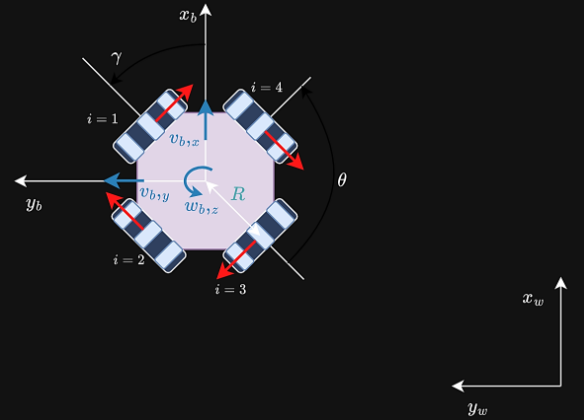
\includegraphics[width=0.65\linewidth]{figures/Chapter 5/Omni_kinematics.png}
    \caption{Omnidirectional Robot Coordinate Frames}
    \label{fig:omni_frames}
\end{figure}

\paragraph{World Frame $\{I\}$}
Fixed inertial frame with $(X_I, Y_I)$ horizontal and $Z_I$ upward. Robot pose: $\mathbf{q} = [x, y, \theta]^T$.

\paragraph{Robot Base Frame $\{B\}$}
Body-fixed frame at geometric center. $x_B$ forward, $y_B$ left, $z_B$ upward. Velocity:
\begin{equation}
\mathbf{v}_B = [v_{b,x}, v_{b,y}, \omega_{b,z}]^T
\label{eq:body_vel}
\end{equation}

\paragraph{Wheel Frames $\{W_i\}$}
Each wheel has driving angle $\alpha_i$ (orientation relative to $x_B$), position angle $\delta_i$ (angle from center to wheel), roller angle $\gamma$, and distance $R$ from robot center.

\subsubsection{Wheel Configuration}

The robot features three omni-wheels separated by 120°:

\begin{table}[H]
\centering
\caption{Three-Wheeled Omni Robot Configuration}
\label{tab:wheel_config}
\begin{tabular}{|l|c|c|c|}
\hline
\textbf{Parameter} & \textbf{Wheel 1} & \textbf{Wheel 2} & \textbf{Wheel 3} \\
\hline
Driving Angle $\alpha_i$ & 270° (--90°) & 150° & 30° \\
\hline
Position Angle $\delta_i$ & 0° & 240° (--120°) & 120° \\
\hline
Roller Angle $\gamma$ & \multicolumn{3}{c|}{0°} \\
\hline
Wheel Radius $r_w$ & \multicolumn{3}{c|}{0.034 m} \\
\hline
Base Radius $R$ & \multicolumn{3}{c|}{0.124 m} \\
\hline
\end{tabular}
\end{table}

\subsubsection{Inverse Kinematics}

The inverse kinematics transforms body velocities to wheel speeds. For a holonomic wheel, motor speed depends on:
\begin{itemize}
    \item \textbf{Longitudinal Velocity} ($v_t$): Motion along rolling direction
    \item \textbf{Lateral Velocity} ($v_p$): Sideways motion compensated by roller angle
\end{itemize}

The fundamental equation:
\begin{equation}
v_{wheel} = v_t + v_p \tan\gamma
\label{eq:wheel_fundamental}
\end{equation}

Velocity at wheel position:
\begin{equation}
\mathbf{v}_{q_{w_i}} = \begin{bmatrix} v_{b,x} + R\omega_{b,z}\sin\delta_i \\ v_{b,y} - R\omega_{b,z}\cos\delta_i \end{bmatrix}
\label{eq:wheel_pos_vel}
\end{equation}

Projecting onto wheel coordinates and simplifying for standard holonomic configuration ($\alpha_i - \delta_i = -90°$) with omni-wheels ($\gamma = 0°$):
\begin{equation}
\omega_i = \frac{1}{r_w} \begin{bmatrix} \cos\alpha_i & \sin\alpha_i & -R \end{bmatrix} \begin{bmatrix} v_{b,x} \\ v_{b,y} \\ \omega_{b,z} \end{bmatrix}
\label{eq:single_wheel_ik}
\end{equation}

The complete inverse kinematics matrix form:
\begin{equation}
\begin{bmatrix} \omega_1 \\ \omega_2 \\ \omega_3 \end{bmatrix} = \frac{1}{r_w} \begin{bmatrix} \cos\alpha_1 & \sin\alpha_1 & -R \\ \cos\alpha_2 & \sin\alpha_2 & -R \\ \cos\alpha_3 & \sin\alpha_3 & -R \end{bmatrix} \begin{bmatrix} v_{b,x} \\ v_{b,y} \\ \omega_{b,z} \end{bmatrix}
\label{eq:ik_general}
\end{equation}

Or in compact form: $\boldsymbol{\omega}_W = \frac{1}{r_w} \mathbf{H} \mathbf{v}_B = \mathbf{J}^{-1} \boldsymbol{\xi}$

Substituting configuration parameters:
\begin{equation}
\begin{bmatrix} \omega_1 \\ \omega_2 \\ \omega_3 \end{bmatrix} = \frac{1}{0.034} \begin{bmatrix} 0 & -1 & -0.124 \\ -\frac{\sqrt{3}}{2} & \frac{1}{2} & -0.124 \\ \frac{\sqrt{3}}{2} & \frac{1}{2} & -0.124 \end{bmatrix} \begin{bmatrix} v_{b,x} \\ v_{b,y} \\ \omega_{b,z} \end{bmatrix}
\label{eq:ik_numerical}
\end{equation}

\paragraph{Global Frame Transformation}
To use global velocities as input:
\begin{equation}
\begin{bmatrix} v_{b,x} \\ v_{b,y} \\ \omega_{b,z} \end{bmatrix} = \begin{bmatrix} \cos\theta & \sin\theta & 0 \\ -\sin\theta & \cos\theta & 0 \\ 0 & 0 & 1 \end{bmatrix} \begin{bmatrix} v_{i,x} \\ v_{i,y} \\ \omega_{i,z} \end{bmatrix}
\label{eq:frame_transform}
\end{equation}

\subsubsection{Forward Kinematics}

Forward kinematics estimates body velocity from measured wheel speeds by inverting the coefficient matrix:
\begin{equation}
\boldsymbol{\xi} = \mathbf{v}_B = r_w \mathbf{H}^{-1} \boldsymbol{\omega}_W = \mathbf{J} \boldsymbol{\omega}_W
\label{eq:fk_compact}
\end{equation}

The general form:
\begin{equation}
\begin{bmatrix} v_{b,x} \\ v_{b,y} \\ \omega_{b,z} \end{bmatrix} = r_w \begin{bmatrix} \frac{2}{3}\cos\alpha_1 & \frac{2}{3}\cos\alpha_2 & \frac{2}{3}\cos\alpha_3 \\ \frac{2}{3}\sin\alpha_1 & \frac{2}{3}\sin\alpha_2 & \frac{2}{3}\sin\alpha_3 \\ -\frac{1}{3R} & -\frac{1}{3R} & -\frac{1}{3R} \end{bmatrix} \begin{bmatrix} \omega_1 \\ \omega_2 \\ \omega_3 \end{bmatrix}
\label{eq:fk_general}
\end{equation}

Substituting configuration parameters:
\begin{equation}
\begin{bmatrix} v_{b,x} \\ v_{b,y} \\ \omega_{b,z} \end{bmatrix} = 0.034 \begin{bmatrix} 0 & -\frac{1}{\sqrt{3}} & \frac{1}{\sqrt{3}} \\ -\frac{2}{3} & \frac{1}{3} & \frac{1}{3} \\ -\frac{1}{0.372} & -\frac{1}{0.372} & -\frac{1}{0.372} \end{bmatrix} \begin{bmatrix} \omega_1 \\ \omega_2 \\ \omega_3 \end{bmatrix}
\label{eq:fk_numerical}
\end{equation}

\subsection{Omnidirectional Interface Driver}
\label{subsec:omni_interface_driver}

The omnidirectional interface driver provides the functional and probabilistic link between motion execution and state estimation. Beyond translating velocity commands into wheel actuation, it produces physically consistent odometry with meaningful uncertainty representation.

\subsubsection{Design Objectives}

The driver explicitly models motion uncertainty from encoder quantization, discretization effects, and execution errors. This enables:
\begin{itemize}
    \item Direct compatibility with probabilistic localization and sensor fusion frameworks
    \item Systematic alignment between simulated and real-world robot performance
    \item Consistent uncertainty propagation throughout the autonomy stack
\end{itemize}

\subsubsection{Functional Requirements}

\begin{enumerate}
    \item \textbf{Velocity Command Interface:} Receive planar velocities in robot body frame via standardized ROS 2 messages
    \item \textbf{Kinematic Transformation:} Map body velocities to wheel velocities supporting full holonomic motion
    \item \textbf{Wheel Command Generation:} Produce synchronized wheel commands for motor control
    \item \textbf{Uncertainty Modeling:} Account for wheel slip, actuator noise, and discretization effects
    \item \textbf{Covariance Propagation:} Compute motion covariance for odometry and sensor fusion
    \item \textbf{Odometry Feedback:} Publish pose increments with associated covariance
    \item \textbf{Real-Time Operation:} Process commands at rates sufficient for stable control
    \item \textbf{Safety Enforcement:} Enforce velocity and acceleration limits
\end{enumerate}

\subsubsection{Design Choices}

A custom driver was developed based on:
\begin{itemize}
    \item \textbf{White-Box Design:} All kinematic transformations, integration steps, and covariance propagation are explicitly implemented---critical for consistency between execution and estimation
    \item \textbf{Computational Efficiency:} Lightweight implementation preserves resources for SLAM and localization
    \item \textbf{Modularity:} Self-contained component with clearly defined interfaces
    \item \textbf{Extensibility:} External configuration of wheel geometry and noise characteristics
\end{itemize}

\subsubsection{Driver Architecture}

The ROS 2 node implements a layered structure:
\begin{enumerate}
    \item Command reception and validation
    \item Kinematic transformation (Eigen3 library)
    \item Odometry integration
    \item Covariance prediction
    \item Publication of wheel commands, odometry, and TF transforms
\end{enumerate}

\paragraph{Twist Representation}
Motion commands use planar twist:
\begin{equation}
\boldsymbol{\xi} = [v_x, v_y, \omega_z]^T
\label{eq:twist_rep}
\end{equation}
This abstraction decouples motion intent from mechanical implementation and provides a foundation for uncertainty propagation.

\paragraph{Kinematic Mapping}
The pipeline transforms twist to wheel velocities: $\boldsymbol{\omega}_w = \mathbf{J}^{-1} \boldsymbol{\xi}$

\subsubsection{Odometry Estimation}

\paragraph{Discrete-Time Integration}
Wheel encoder measurements are converted to incremental displacements and mapped to body-frame motion:
\begin{equation}
\Delta \mathbf{x}_b = [\Delta x, \Delta y, \Delta \theta]^T
\label{eq:body_increment}
\end{equation}

Using Euler integration, the global pose updates:
\begin{equation}
\mathbf{x}_{k+1} = \mathbf{x}_k + \mathbf{R}(\theta_k) \begin{bmatrix} \Delta x \\ \Delta y \end{bmatrix} + \begin{bmatrix} 0 \\ 0 \\ \Delta \theta \end{bmatrix}
\label{eq:euler_integration}
\end{equation}
where $\mathbf{R}(\theta_k)$ is the planar rotation matrix.

\paragraph{Coordinate Frames}
The driver publishes the \texttt{odom} $\rightarrow$ \texttt{base\_link} transform, representing estimated pose relative to a locally fixed reference. This continuous estimate is fused with global corrections from localization algorithms.

\subsubsection{Odometry Covariance Modeling}

\paragraph{Motivation}
Probabilistic localization (EKF, AMCL) requires accurate motion covariance. Deterministic odometry leads to overconfident predictions and estimator inconsistency.

\paragraph{Encoder Quantization Noise}
Each encoder provides discrete measurements with resolution defined by pulses per revolution (PPR). The smallest angular increment:
\begin{equation}
\Delta \phi = \frac{2\pi}{\text{PPR}}
\label{eq:encoder_resolution}
\end{equation}

Assuming uniform quantization, the angular measurement variance:
\begin{equation}
\sigma_\phi^2 = \frac{(\Delta \phi)^2}{12}
\label{eq:angular_variance}
\end{equation}

Propagated to wheel displacement:
\begin{equation}
\sigma_s^2 = r^2 \sigma_\phi^2
\label{eq:displacement_variance}
\end{equation}

\paragraph{Multi-Encoder Covariance}
For $N$ wheels with independent quantization noise:
\begin{equation}
\boldsymbol{\Sigma}_s = \text{diag}(\sigma_{s_1}^2, \sigma_{s_2}^2, \ldots, \sigma_{s_N}^2)
\label{eq:wheel_covariance}
\end{equation}

\paragraph{Robot Motion Uncertainty}
Through the forward kinematic Jacobian $\mathbf{J}$:
\begin{equation}
\boldsymbol{\Sigma}_{\Delta x} = \mathbf{J} \boldsymbol{\Sigma}_s \mathbf{J}^T
\label{eq:motion_covariance}
\end{equation}

This produces correlated uncertainty due to geometric coupling in omnidirectional platforms.

\paragraph{Twist Covariance}
For Kalman prediction, displacement covariance converts to velocity covariance:
\begin{equation}
\boldsymbol{\Sigma}_{\text{twist}} = \frac{1}{(\Delta t)^2} \boldsymbol{\Sigma}_{\Delta x}
\label{eq:twist_covariance}
\end{equation}

\subsubsection{Kalman Prediction for Covariance Propagation}

\paragraph{State Integration}
At each time step, the global pose updates:
\begin{align}
\Delta x &= (v_x \cos\theta_k - v_y \sin\theta_k) \Delta t \label{eq:delta_x} \\
\Delta y &= (v_x \sin\theta_k + v_y \cos\theta_k) \Delta t \label{eq:delta_y} \\
\Delta \theta &= \omega_z \Delta t \label{eq:delta_theta}
\end{align}

\paragraph{State Jacobian}
The Jacobian with respect to state $\mathbf{x} = [x, y, \theta]^T$:
\begin{equation}
\mathbf{F}_k = \begin{bmatrix} 1 & 0 & (-v_x \sin\theta_k - v_y \cos\theta_k) \Delta t \\ 0 & 1 & (v_x \cos\theta_k - v_y \sin\theta_k) \Delta t \\ 0 & 0 & 1 \end{bmatrix}
\label{eq:state_jacobian}
\end{equation}

\paragraph{Control Jacobian}
The Jacobian with respect to control $\mathbf{u}_k = [v_x, v_y, \omega_z]^T$:
\begin{equation}
\mathbf{G}_k = \begin{bmatrix} \cos\theta_k \Delta t & -\sin\theta_k \Delta t & 0 \\ \sin\theta_k \Delta t & \cos\theta_k \Delta t & 0 \\ 0 & 0 & \Delta t \end{bmatrix}
\label{eq:control_jacobian}
\end{equation}

\paragraph{Process Noise}
\begin{equation}
\mathbf{Q}_k = \mathbf{G}_k \boldsymbol{\Sigma}_{\text{twist}} \mathbf{G}_k^T
\label{eq:process_noise}
\end{equation}

\paragraph{Covariance Prediction}
\begin{equation}
\mathbf{P}_{k+1} = \mathbf{F}_k \mathbf{P}_k \mathbf{F}_k^T + \mathbf{Q}_k
\label{eq:covariance_prediction}
\end{equation}

This captures both propagation of existing uncertainty and injection of new uncertainty from motion execution. Higher $\mathbf{Q}_k$ indicates greater process model uncertainty.

The omnidirectional kinematic model enables heading-independent translation, a critical capability for navigation in cluttered environments. Simulation validation of this capability is presented in Section~\ref{subsec:omni_motion_validation}, demonstrating pure lateral motion while maintaining constant heading.
\newpage
\section{Autonomous System Node Structure}
\label{sec:autonomous_system_nodes}

This section provides a consolidated view of the complete autonomous system architecture, synthesizing the individual components described throughout this chapter into a unified data flow diagram.

\subsection{Single Robot Architecture}

A detailed breakdown of the internal software pipeline for a single robot instance is shown in Figure \ref{fig:deep_dive}. This diagram illustrates the three-layer architecture: Perception, Autonomy, and Control.

\begin{figure}[H]
    \centering
    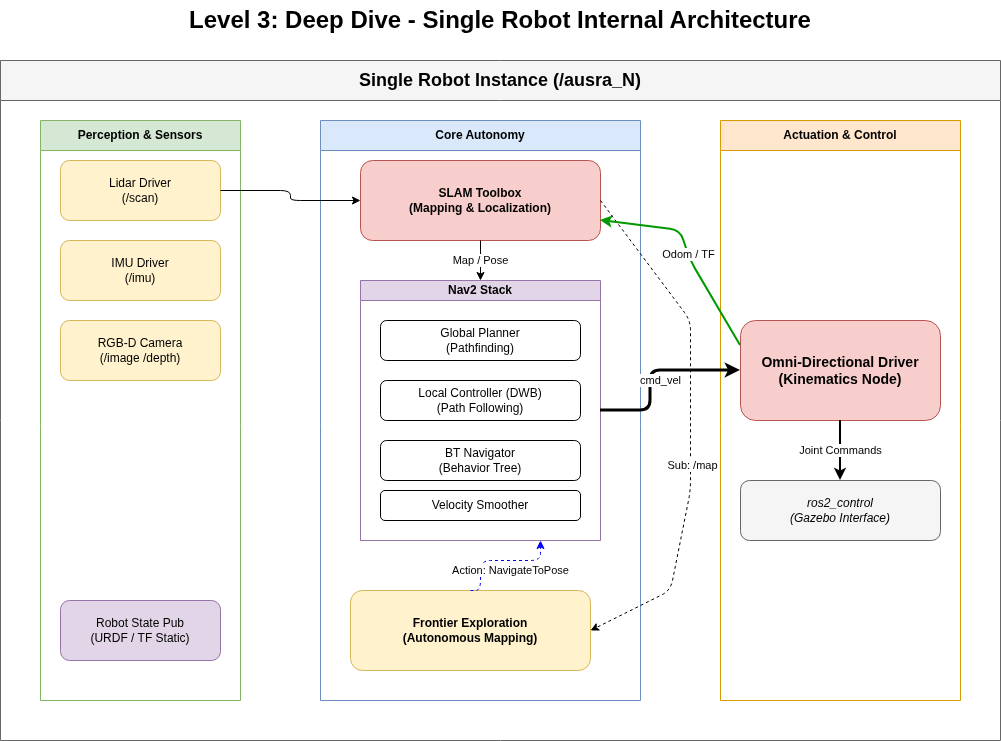
\includegraphics[width=0.95\linewidth]{figures/Chapter 5/Deep_dive_single_robot.png}
    \caption{Level 3: Deep Dive - Single Robot Internal Architecture}
    \label{fig:deep_dive}
\end{figure}

\subsection{Data Flow Pipeline}

\subsubsection{Perception Layer}
The perception layer acquires and processes raw sensor data:
\begin{itemize}
    \item \textbf{LiDAR Driver:} Publishes 2D laser scans at 5.5 Hz on \texttt{/scan}
    \item \textbf{IMU Driver:} Publishes inertial data at 100 Hz on \texttt{/imu/data\_raw}
    \item \textbf{Depth Camera:} Publishes point clouds and RGB images for obstacle detection
    \item \textbf{Wheel Encoders:} Provide tick counts to the omni\_driver for odometry computation
\end{itemize}

\subsubsection{Localization and Mapping Layer}
This layer fuses sensor data to build environmental understanding:
\begin{itemize}
    \item \textbf{EKF Node:} Fuses IMU and wheel odometry to produce filtered state estimates on \texttt{/odometry/filtered}
    \item \textbf{SLAM Toolbox:} Consumes laser scans and odometry to build the occupancy grid map and refine robot pose through scan matching
    \item \textbf{TF Broadcaster:} Maintains the transform tree connecting all coordinate frames
\end{itemize}

\subsubsection{Planning and Navigation Layer}
The Nav2 stack handles high-level decision making:
\begin{itemize}
    \item \textbf{Behavior Tree Navigator:} Orchestrates the navigation task using a behavior tree, handling recovery actions and goal management
    \item \textbf{Planner Server (SmacPlanner2D):} Computes globally optimal paths using A* search on the costmap
    \item \textbf{Controller Server (DWB):} Generates local trajectories that follow the global path while avoiding dynamic obstacles
    \item \textbf{Costmap 2D:} Maintains layered costmaps (static, obstacle, inflation) for planning
\end{itemize}

\subsubsection{Control Layer}
The control layer executes velocity commands:
\begin{itemize}
    \item \textbf{Omni Driver:} Converts body-frame velocities ($v_x$, $v_y$, $\omega$) to wheel angular velocities using the inverse kinematics matrix (Equation \ref{eq:ik_general})
    \item \textbf{micro-ROS Agent:} Bridges ROS 2 DDS to the ESP32 via UART at 921600 baud
    \item \textbf{ESP32 Firmware:} Executes PID control loops for each motor at 100 Hz
\end{itemize}

\subsection{Topic Summary}

Table \ref{tab:topic_summary} provides a comprehensive list of the key ROS 2 topics in the autonomous system.

\begin{table}[H]
\centering
\caption{Autonomous System Topic Summary}
\label{tab:topic_summary}
\begin{tabular}{|l|l|c|l|}
\hline
\textbf{Topic} & \textbf{Message Type} & \textbf{Rate} & \textbf{Purpose} \\
\hline
\texttt{/scan} & sensor\_msgs/LaserScan & 5.5 Hz & LiDAR data \\
\texttt{/imu/data\_raw} & sensor\_msgs/Imu & 100 Hz & IMU measurements \\
\texttt{/odometry/filtered} & nav\_msgs/Odometry & 50 Hz & EKF state estimate \\
\texttt{/map} & nav\_msgs/OccupancyGrid & 1 Hz & SLAM output \\
\texttt{/goal\_pose} & geometry\_msgs/PoseStamped & Event & Navigation goal \\
\texttt{/plan} & nav\_msgs/Path & Event & Global path \\
\texttt{/cmd\_vel} & geometry\_msgs/Twist & 20 Hz & Velocity command \\
\texttt{/wheel/odom} & nav\_msgs/Odometry & 100 Hz & Wheel odometry \\
\texttt{/tf} & tf2\_msgs/TFMessage & 100 Hz & Transform tree \\
\hline
\end{tabular}
\end{table}

The complete autonomous stack integrating all these components was validated through comprehensive simulation testing, achieving 95\% map coverage in under 1 minute 40 seconds. Detailed integration test results are presented in Section~\ref{subsec:complete_stack_test}.

\section{Robot Description (URDF)}
\label{sec:urdf}

The physical description of the robot is defined using the Unified Robot Description Format (URDF), augmented by the Xacro macro system for modularity and multi-robot support.

\subsection{Xacro Architecture}

The robot description is split into modular files:
\begin{itemize}
    \item \texttt{robot.urdf.xacro}: Top-level entry point accepting arguments (e.g., \texttt{robot\_name}) and including sub-components
    \item \texttt{robot\_core.xacro}: Defines physical chassis, wheels, and joints with dynamic namespacing support
    \item \texttt{sensors.xacro}: Attaches sensor plugins (LiDAR, Camera, IMU) to the base link
    \item \texttt{gazebo\_classic.xacro}: Defines Gazebo-specific tags (friction, materials) and loads \texttt{ros\_control} plugins
\end{itemize}

\subsection{Model Generation}

At runtime, the Xacro engine generates pure XML URDF. For example, spawning \texttt{ausra\_1}:
\begin{verbatim}
xacro robot.urdf.xacro robot_name:=ausra_1
\end{verbatim}

This replaces all \texttt{\$\{robot\_name\}} occurrences with \texttt{ausra\_1}, creating a unique TF tree (e.g., \texttt{ausra\_1\_base\_link}, \texttt{ausra\_1\_wheel\_1}) that allows multiple robots to coexist in the same TF buffer.

See Appendix \ref{app:urdf_code} for the core chassis definition.

\section{Future Work and Research}
\label{sec:ch5_future_work}

The architecture is designed to support advanced collaborative features currently in research and development.

\subsection{Collaborative Algorithms (Planned)}

\begin{itemize}
    \item \textbf{Single Pose Graph SLAM:} All robots contribute to a unified constraint graph, allowing Loop Closures triggered by Agent A to correct Agent B's pose drift, creating a mathematically consistent global map
    \item \textbf{mTSP Task Allocation:} Integration of a centralized ``Multiple Traveling Salesman Problem'' solver (using Google OR-Tools) to replace frontier assignment with globally optimal scheduling, minimizing total coverage time
    \item \textbf{Lazy Traffic Controller:} Decentralized avoidance using ``Velocity Obstacles'' where agents broadcast velocity vectors to neighbors, computing collision-free trajectories in velocity space without central planning
\end{itemize}

\subsection{Advanced Perception}

Future upgrades include:
\begin{itemize}
    \item Inter-Process Communication (IPC) for high-frequency camera data handling
    \item AprilTag detection for automated victim identification and localization
\end{itemize}


\include{chapters/chapter6_results}
\include{chapters/chapter7_conclusion}

% --- Back Matter ---

% References
\printbibliography[heading=bibintoc, title={References}]

% Appendices
\appendix
% ============================================================================
% Appendices
% ============================================================================

\chapter{Simulation World Construction}
\label{app:sim_code}

This appendix provides an example of the SDF (Simulation Description Format) code used to generate the test worlds. The following listing describes a standard room environment with defined physics, lighting, and static obstacles.

\begin{lstlisting}[language=XML, caption={SDF World Definition Example (room\_1.sdf)}]
<?xml version="1.0" ?>
<sdf version="1.6">
  <world name="room_1">
    
    <!-- Physics settings -->
    <physics type="ode">
      <max_step_size>0.001</max_step_size>
      <real_time_factor>1</real_time_factor>
      <real_time_update_rate>1000</real_time_update_rate>
    </physics>

    <!-- Scene settings -->
    <scene>
      <ambient>0.4 0.4 0.4 1</ambient>
      <background>0.7 0.7 0.7 1</background>
      <shadows>true</shadows>
    </scene>

    <!-- Ground plane -->
    <model name="ground_plane">
      <static>true</static>
      <link name="link">
        <collision name="collision">
          <geometry>
            <plane>
              <normal>0 0 1</normal>
              <size>20 20</size>
            </plane>
          </geometry>
        </collision>
        <visual name="visual">
          <geometry>
            <plane>
              <normal>0 0 1</normal>
              <size>20 20</size>
            </plane>
          </geometry>
        </visual>
      </link>
    </model>

    <!-- Example Obstacle: Red Box -->
    <model name="obstacle_red">
      <static>true</static>
      <pose>-2.5 2.5 0.25 0 0 0</pose>
      <link name="link">
        <collision name="collision">
          <geometry>
            <box><size>0.5 0.5 0.5</size></box>
          </geometry>
        </collision>
        <visual name="visual">
          <geometry>
            <box><size>0.5 0.5 0.5</size></box>
          </geometry>
          <material>
            <ambient>0.8 0.1 0.1 1</ambient>
            <diffuse>0.8 0.1 0.1 1</diffuse>
          </material>
        </visual>
      </link>
    </model>

  </world>
</sdf>
\end{lstlisting}

\chapter{Robot Description Listing}
\label{app:urdf_code}

This appendix contains the core Xacro definition for the robot chassis. Note the use of the \texttt{robot\_name} parameter to enable dynamic namespacing for multi-robot swarms.

\begin{lstlisting}[language=XML, caption={Robot Core Xacro Definition (robot\_core.xacro)}]
<?xml version="1.0"?>
<robot xmlns:xacro="http://www.ros.org/wiki/xacro">

  <xacro:macro name="robot_core" params="robot_name">
  
    <!-- Base Link Definition -->
    <link name="${robot_name}_base_link">
      <visual>
        <geometry>
          <mesh filename="package://ausrabot_description/meshes/base_link.STL" />
        </geometry>
        <material name="body_color">
          <color rgba="0.792 0.819 0.933 1" />
        </material>
      </visual>
      <collision>
        <geometry>
          <cylinder radius="0.13" length="0.10"/>
        </geometry>
      </collision>
      <inertial>
        <mass value="0.749591825708612" />
        <inertia ixx="0.0056" ixy="0.0" ixz="0.0" 
                 iyy="0.0054" iyz="0.0" izz="0.0095" />
      </inertial>
    </link>

    <!-- Omni Wheel 1 Definition -->
    <link name="${robot_name}_wheel_1">
      <visual>
        <geometry>
          <mesh filename="package://ausrabot_description/meshes/wheel_1.STL" />
        </geometry>
      </visual>
      <collision>
        <geometry>
          <cylinder radius="0.0325" length="0.03"/>
        </geometry>
      </collision>
    </link>

    <!-- Joint 1: Connects Wheel 1 to Base -->
    <joint name="${robot_name}_joint_1" type="continuous">
      <origin xyz="0.12368 -0.00013859 -0.019" rpy="1.5708 0 1.5708" />
      <parent link="${robot_name}_base_link" />
      <child link="${robot_name}_wheel_1" />
      <axis xyz="0 0 1" />
    </joint>

    <!-- Additional Wheels (2 and 3) defined similarly -->
    
  </xacro:macro>
</robot>
\end{lstlisting}

\chapter{Code Listings}
\label{app:code}

This appendix contains key software implementations used in the AUSRA system.

\section{Frontier Exploration Logic}
\label{code:frontier_api}

The following C++ implementation from \texttt{ausra\_frontier\_exploration} demonstrates the custom logic for identifying and clustering safe frontiers.

\begin{lstlisting}[language=C++, caption={Frontier Search and Safety Filtering}]
// src/frontier_search.cpp
std::vector<Frontier> FrontierSearch::searchFromMap(
  const nav_msgs::msg::OccupancyGrid & costmap,
  double robot_x, double robot_y)
{
  // ... [Initialization code omitted] ...

  // Scan for frontier cells (free cells adjacent to unknown)
  for (int y = 1; y < height_ - 1; ++y) {
    for (int x = 1; x < width_ - 1; ++x) {
      if (isFrontierCell(data, x, y)) {
        // Safety Check 1: Count obstacle neighbors
        int obs_count = 0;
        // ... [Neighbor loop omitted] ...
        
        // Filter: max 1 obstacle neighbor to avoid tight corners
        if (obs_count <= 1) {
          // Safety Check 2: Check 1m radius safety (98% safe cells)
          if (isSafeArea(data, x, y)) {
            frontier_cells.emplace_back(x, y);
          }
        }
      }
    }
  }

  return clusterFrontiers(frontier_cells, robot_x, robot_y);
}

// Logic to check 1m radius safety ratio
bool FrontierSearch::isSafeArea(
    const std::vector<int8_t> & data, int x, int y) const
{
  int radius_cells = static_cast<int>(1.0 / resolution_);
  // ... [Loop bounds calculation] ...
  
  for (int cy = y_min; cy < y_max; ++cy) {
    for (int cx = x_min; cx < x_max; ++cx) {
      total++;
      int8_t val = data[toIndex(cx, cy)];
      if (val == 0 || val == -1) {  // Free or unknown count as safe
        safe++;
      }
    }
  }
  
  // Only accept if safety ratio matches configuration (default 0.98)
  return (static_cast<double>(safe) / total) >= safety_ratio_;
}
\end{lstlisting}

\begin{lstlisting}[language=C++, caption={Frontier Clustering and Goal Adjustment}]
// src/frontier_search.cpp - clusterFrontiers method

// BFS logic to cluster adjacent frontier cells...
// ...

// Calculate Centroid
double centroid_grid_x = sum_x / cluster.size();
double centroid_grid_y = sum_y / cluster.size();

// Goal Pullback Logic:
// Pull the goal 0.5m back towards the known free space 
// to ensure A* reachability
int pullback_cells = static_cast<int>(0.5 / resolution_);
int goal_grid_x = static_cast<int>(centroid_grid_x - dir_x * pullback_cells);
int goal_grid_y = static_cast<int>(centroid_grid_y - dir_y * pullback_cells);

// Compute Cost Function for selection
// Prefer closer frontiers (potential_scale) and larger frontiers (gain_scale)
f.cost = potential_scale * f.min_distance - gain_scale * f.size;
\end{lstlisting}

\section{Navigation Configuration}
\label{code:nav_config}

The system uses standard Nav2 plugins configured specifically for multi-robot omnidirectional navigation.

\subsection{SmacPlanner (A*) Configuration}

The \texttt{SmacPlanner2D} provides efficient A* planning on large costmaps.

\begin{lstlisting}[language=bash, caption={SmacPlanner2D A* Configuration}]
planner_server:
  ros__parameters:
    planner_plugins: ["GridBased"]
    GridBased:
      plugin: "nav2_smac_planner/SmacPlanner2D"
      tolerance: 0.5                     # Goal tolerance
      downsample_costmap: false          # Full resolution for safety
      allow_unknown: true                # Plan through unknown space
      max_iterations: 1000000            # High iteration count for large maps
      cost_travel_multiplier: 50.0       # Heavy penalty for high-cost areas
      use_final_approach_orientation: false # Direction agnostic for Omni robot
\end{lstlisting}

\subsection{DWB Local Controller Configuration}

The local controller is tuned for holonomic motion, sampling velocities in X and Y directions.

\begin{lstlisting}[language=bash, caption={DWB Holonomic Controller Configuration}]
controller_server:
  ros__parameters:
    # DWB Controller for OMNIDIRECTIONAL/HOLONOMIC robot
    FollowPath:
      plugin: "dwb_core::DWBLocalPlanner"
      
      # Trajectory Generation
      min_vel_x: -0.35
      max_vel_x: 0.35
      min_vel_y: -0.35              # Full lateral motion enabled
      max_vel_y: 0.35
      max_vel_theta: 1.0
      
      # Sampling strategy for Holonomic Motion
      vx_samples: 15
      vy_samples: 15                 # Sample lateral velocities
      vtheta_samples: 8              # Minimize rotation samples
      
      # Critics Configuration
      critics: ["Oscillation", "ObstacleFootprint", 
                "PathDist", "GoalDist", "Twirling"]
      
      # Twirling Critic: Heavily penalize unnecessary rotation
      Twirling:
        scale: 10.0
      
      # ObstacleFootprint: Critical safety check
      ObstacleFootprint:
        scale: 100.0                 # Highest priority
\end{lstlisting}

\section{Motor Control Firmware}
\label{code:motor_control}

\begin{lstlisting}[language=C, caption={PID Motor Controller Implementation}]
// PID Controller Structure
typedef struct {
    float Kp, Ki, Kd;
    float integral;
    float prev_error;
    float dt;
} PID_Controller;

float pid_compute(PID_Controller* pid, float error) {
    pid->integral += error * pid->dt;
    float derivative = (error - pid->prev_error) / pid->dt;
    pid->prev_error = error;
    
    return pid->Kp * error + 
           pid->Ki * pid->integral + 
           pid->Kd * derivative;
}
\end{lstlisting}

\chapter{Bill of Materials}
\label{app:bom}

The following table presents the complete Bill of Materials (BOM) for a single AUSRA robot unit. All prices are listed in Egyptian Pounds (EGP) with USD equivalent calculated at approximately 50 EGP/USD.

\section{Structural Components}

\begin{longtable}{|c|p{4cm}|c|c|c|}
\hline
\textbf{Item} & \textbf{Description} & \textbf{Qty} & \textbf{Unit (EGP)} & \textbf{Total (EGP)} \\
\hline
\endhead
1 & Ground Plate (3D Printed) - Structural foundation for motors and drivers & 1 & 250 & 250 \\
2 & Middle Plate (3D Printed) - Support for battery, ESP32, and drivers & 1 & 150 & 150 \\
3 & Upper Plate (3D Printed) - Mounting for Jetson and sensors & 1 & 150 & 150 \\
4 & Cylindrical Wall (3D Printed) - Protective enclosure & 1 & 1,200 & 1,200 \\
5 & Cover (3D Printed) - Top protection for LiDAR assembly & 1 & 300 & 300 \\
6 & Camera Bracket (3D Printed) - OAK-D Lite mounting fixture & 1 & 150 & 150 \\
7 & Battery Mount (3D Printed) - Custom battery pack fixture & 1 & 100 & 100 \\
\hline
\multicolumn{4}{|r|}{\textbf{Structural Subtotal}} & \textbf{2,300} \\
\hline
\end{longtable}

\section{Mechanical Components}

\begin{longtable}{|c|p{4cm}|c|c|c|}
\hline
\textbf{Item} & \textbf{Description} & \textbf{Qty} & \textbf{Unit (EGP)} & \textbf{Total (EGP)} \\
\hline
\endhead
8 & Omni Wheel (58mm, Custom Made) - Holonomic locomotion & 3 & 400 & 1,200 \\
9 & Wheel Shaft (Custom Machined) - Torque transmission & 3 & 15 & 45 \\
10 & Bearing Bracket (Ready Made) - Shaft alignment & 3 & 25 & 75 \\
11 & Bearing KFL08 - Friction reduction & 3 & 70 & 210 \\
12 & Flexible Coupler - Motor-to-shaft linkage & 3 & 200 & 600 \\
13 & Motor Holder (Ready Made) - Actuation support & 3 & 25 & 75 \\
14 & Worm Gear DC Motor (TS-32GZ370-5300) - Locomotion actuator & 3 & 850 & 2,550 \\
15 & Spacers (M3, various lengths) - Vertical standoffs & 16 & 10 & 160 \\
16 & Fastening Consumables (Bolts, Nuts) - Assembly hardware & -- & -- & 100 \\
\hline
\multicolumn{4}{|r|}{\textbf{Mechanical Subtotal}} & \textbf{5,015} \\
\hline
\end{longtable}

\section{Electrical Components}

\begin{longtable}{|c|p{4cm}|c|c|c|}
\hline
\textbf{Item} & \textbf{Description} & \textbf{Qty} & \textbf{Unit (EGP)} & \textbf{Total (EGP)} \\
\hline
\endhead
17 & Dual Stage Buck Module (LM2596) - 20V$\rightarrow$12V regulation & 2 & 300 & 600 \\
18 & Cytron MDD3A Motor Driver - PWM to high-power conversion & 2 & 900 & 1,800 \\
19 & Battery (Total P20S Power Kit) - High-current power source & 1 & 1,000 & 1,000 \\
20 & Charging Port (GX16 4-Pin) - External charging interface & 1 & 45 & 45 \\
21 & Wire Connector (SPL-62, 2-in 6-out) - Power distribution & 1 & 40 & 40 \\
22 & Safety Toggle Switch (E-TEN1122 DPDT) - Three-state failsafe & 1 & 30 & 30 \\
23 & Assembly Consumables (Wires, Terminals, Heat Shrink) & -- & -- & 500 \\
\hline
\multicolumn{4}{|r|}{\textbf{Electrical Subtotal}} & \textbf{4,015} \\
\hline
\end{longtable}

\section{Compute and Control}

\begin{longtable}{|c|p{4cm}|c|c|c|}
\hline
\textbf{Item} & \textbf{Description} & \textbf{Qty} & \textbf{Unit (EGP)} & \textbf{Total (EGP)} \\
\hline
\endhead
24 & ESP32-S3-N16R8 - Low-level microcontroller (micro-ROS, kinematics) & 1 & 400 & 400 \\
25 & ESP32-S3 Shield (Custom PCB) - Signal distribution board & 1 & 300 & 300 \\
26 & NVIDIA Jetson Orin Nano Dev Kit - Primary compute platform & 1 & 11,000 & 11,000 \\
\hline
\multicolumn{4}{|r|}{\textbf{Compute Subtotal}} & \textbf{11,700} \\
\hline
\end{longtable}

\section{Sensors}

\begin{longtable}{|c|p{4cm}|c|c|c|}
\hline
\textbf{Item} & \textbf{Description} & \textbf{Qty} & \textbf{Unit (EGP)} & \textbf{Total (EGP)} \\
\hline
\endhead
27 & RPLIDAR A1 - 360° 2D laser scanner for SLAM & 1 & 7,500 & 7,500 \\
28 & OAK-D Lite Depth Camera - Spatial AI and depth perception & 1 & 7,500 & 7,500 \\
29 & MPU-9250 9-Axis IMU - Inertial navigation sensor & 1 & 700 & 700 \\
30 & IMU Interface PCB (Custom Made) - Sensor signal routing & 1 & 100 & 100 \\
\hline
\multicolumn{4}{|r|}{\textbf{Sensors Subtotal}} & \textbf{15,800} \\
\hline
\end{longtable}

\section{Cost Summary}

\begin{table}[H]
\centering
\caption{Per-Robot Cost Summary}
\label{tab:bom_summary_appendix}
\begin{tabular}{|l|r|r|r|}
\hline
\textbf{Category} & \textbf{EGP} & \textbf{USD} & \textbf{Percentage} \\
\hline
Structural Components & 2,300 & 46 & 5.9\% \\
Mechanical Components & 5,015 & 100 & 12.9\% \\
Electrical Components & 4,015 & 80 & 10.3\% \\
Compute and Control & 11,700 & 234 & 30.1\% \\
Sensors & 15,800 & 316 & 40.7\% \\
\hline
\textbf{Grand Total} & \textbf{38,830} & \textbf{\$777} & \textbf{100\%} \\
\hline
\end{tabular}
\end{table}

\textbf{Note:} The above pricing reflects current Egyptian market rates (January 2026). International pricing may vary. The \$420 USD figure cited in the main text represents optimized bulk purchasing and excludes premium sensors (OAK-D Lite, RPLIDAR A1) which can be substituted with lower-cost alternatives for budget-constrained deployments.


% Arabic Summary (ASU Specific)
% ============================================================================
% Arabic Summary
% ============================================================================

% Arabic summary content removed - pdflatex does not support Arabic text.
% Use XeLaTeX or LuaLaTeX with appropriate fonts for Arabic content.


\end{document}
